\documentclass[]{aa}

\usepackage{graphicx}
\usepackage{txfonts}
\usepackage{natbib}

\bibpunct{(}{)}{;}{a}{}{,} % to follow the A&A style

% shortcut to typeset a 2x2 matrix... there are a lot of these
\newcommand{\matrixtt}[4]{\left( \begin{array}{cc}#1&#2\\#3&#4\\\end{array} \right)}

% typographical conventions
% symbol used to indicate the Hermitian transpose
\newcommand{\herm}{H}
%% other common usage is: \newcommand{\herm}{\dagger}
% this typesets a Jones matrix
\newcommand{\jones}[2]{\vec {#1}_{#2}}
% this typesets an inverse Jones matrix
\newcommand{\jonesinv}[2]{\vec {#1}^{-1}_{#2}}
% this typesets a conjugate-transpose Jones matrix
\newcommand{\jonesT}[2]{\vec {#1}^{\herm}_{#2}}
% this typesets an inverse conjugate-transpose Jones matrix
\newcommand{\jonesTinv}[2]{\vec {#1}^{{\herm}-1}_{#2}}
% this typesets a coherency matrix
\newcommand{\coh}[2]{\mathsf{{#1}}_{{#2}}}

\newcommand{\EDIT}[1]{{\bf #1}}


\begin{document}


\title{Revisiting the Measurement Equation: Understanding And Calibrating Direction-Dependent Effects In Radio Interferometers}

\author{O.M.\ Smirnov}

\institute{Netherlands Institute for Radio Astronomy (ASTRON)\\
  P.O. Box 2, 7990AA Dwingeloo, The Netherlands \\
  \email{smirnov@astron.nl}}

\date{}

\titlerunning{Measurement Equation \& Direction-Dependent Effects}
\authorrunning{O.M.\ Smirnov}

\abstract%
%optional context
{Since its formulation by Hamaker et al., the radio interferometer measurement equation (RIME) 
has provided a rigorous mathematical basis for the development of novel calibration methods and 
techniques, including various approaches to the problem of direction-dependent effects (DDEs). 
However, acceptance of the RIME in the radioastronomical community at large has been slow, which is
partially due to the limited availability of software to exploit its power, and the sparsity of 
practical results. This needs to change urgently.}
%aims
{This work aims to place recent developments in the treatment of DDEs into one RIME-based mathematical 
framework, and to demonstrate the ease with which the various effects can be described and understood. 
It also demonstrates the benefits of a RIME-based approach to calibration, by presenting 
an example of extremely high-dynamic range calibration of WSRT observations of 3C147 at 21 cm, with 
full treatment of DDEs. 
}
%methods
{The first part of this paper re-derives the RIME from first principles, extends the formalism to
the full-sky case, and incorporates DDEs. It then uses the formalism to describe self-calibration, both with 
a full RIME, and with the approximate equations of older software packages, and shows how this is affected 
by DDEs. It then gives an overview of real-life DDEs and proposed methods of dealing with them. Finally, it 
shows how some of these methods can be applied self-calibration of 21cm WSRT observations, and analyzes the results.
}%
%results
{Applying the RIME to calibration of WSRT data results in an image of the field around 3C147 with a very high dynamic 
range (1.6 million), and none of the off-axis artifacts that plague regular selfcal. The resulting differential gain solutions contain information on DDEs and errors in the sky model. The paper shows that sources as faint as 2 mJy 
yield meaningful DDE solutions, and thus can be used as potential calibration beacons. 
}%
%optional conclusions
{}

\keywords{Methods: numerical - Methods: analytical - Methods: data analysis - Techniques:
interferometric - Techniques: polarimetric}

\maketitle

\section*{Introduction}

The Measurement Equation of a generic radio interferometer (henceforth referred to as the RIME) was formulated by \citet{ME1} after almost 50 years of radio astronomy. Prior to the RIME, mathematical models of radio interferometers (as implemented by a number of software packages such as AIPS, Miriad, NEWSTAR, DIFMAP) were somewhat \emph{ad hoc} and approximate. Despite this (and in part thanks to the careful design of existing instruments), the technique of {\em selfcalibration} \citep{Cornwell:selfcal} has allowed radio astronomers to achieve spectacular results. However, by the time the RIME was formulated, even older and well-understood instruments such as the Westerbork Synthesis Radio Telescope (WSRT) and the Very Large Array (VLA) were beginning to expose the limitations of these approximate models. New instruments (and upgrades of older observatories), such as the current crop of Square Kilometer Array \citep{Schilizzi:SKA} ``pathfinders'', and indeed the SKA itself, were already beginning to loom on the horizon. These new instruments exhibit far more subtle and elaborate observational effects, due not only to their greately increased sensitivity, but also to new features of their design. In particular, while traditional selfcal only deals with direction-independent effects (DIEs), calibration of these new instruments requires us to deal with direction-dependent effects (DDEs), or effects that vary across the field of view (FoV) of the instrument. Following \citet{meqtrees}, I shall refer to \emph{generations} of calibration methods, with first-generation calibration (1GC) predating selfcal, 2GC being traditional selfcal as implemented by the abovementioned packages, and 3GC corresponding to the burgeoning field of DDE-related methods and algorithms. 

It is indeed quite fortunate that the emergence of the RIME formalism has provided us with a complete and elegant mathematical framework for dealing with observational effects, and ultimately DDEs. Oddly enough, outside of a small community of algorithm developers that have enthusiastically accepted the formalism and put it to good use, uptake of RIME by radio astronomers at large has been slow. Even more worryingly, almost 15 years after the first publication, the formalism is hardly ever taught to the new generation of students. This is worrying, because in my estimation, the RIME should be the cornerstone of every entry-level interferometry course! In part, this slow acceptance has been shaped by the availability of software. Today's radio astronomers rely almost exclusively on the 2GC software packages mentioned above, whose internal paradigms are rooted in the selfcal developments of the 1980s and lack an explicit RIME.\footnote{All 2GC packages do use some specific and limited form of the RIME implicitly. This will be discussed further in Sect.~\ref{sec:calibration}.} \EDIT{On the other hand, relatively few observations were really sensitive enough to push the limits of (or have their science goals compromised by) 2GC.}
The continued success of legacy packages has meant that the {\em thinking} about interferometry and calibration has still been largely shaped by pre-RIME paradigms. What has not helped this situation is that new software exploiting the power of the RIME has been slow to emerge, and practical results even more so (but see Sect.~\ref{sec:3C147} of this paper).  

On the other hand, from my personal experience of teaching the RIME at several workshops, once the penny drops, people tend to describe it in terms such as ``obvious'', ``simple'', ``intuitive'', ``elegant'' and ``powerful''. This points at an explanatory gap in the literature. The first part of this paper therefore tries to address this gap, recasting existing ideas into one consistent mathematical framework, and showing where other approaches to the RIME fit in. Section~\ref{sec:derivation} revisits the ideas of the original RIME papers I \citep{ME1} and IV \citep{ME4}, deriving the RIME from first principles. It then demonstrates how the fundamentals of interferometry itself (and the van Cittert-Zernike theorem in particular) follow from the RIME (rather than the other way around!), in the process showing how the formalism can incorporate DDEs. This section also looks at alternative formulations of the RIME and their practical implications, and shows where they fit into the formalism. It also tries to clear up some controversies and misunderstandings that have accumulated over the years. Section~\ref{sec:calibration} discusses calibration in RIME terms, and explicates the links between the RIME and 2GC implementations of selfcal. 

Section~\ref{sec:ddes} discusses the subject of DDEs, and places existing approaches into the mathematical framework developed in the preceding sections. DDEs were outside the scope of the original RIME publications, but various authors have been incorporating them into the RIME since. \citet{Rau:DDEs} and \citet{SB:calibration-low-freq} provide an in-depth review of these developments, especially as pertaining to imaging and deconvolution. The above authors have developed a description of DDEs using the $4\times4$ Mueller matrix and coherency vector formalism of Paper I. The $4\times4$ formalism has also been included in the 2nd edition of \citet*[Sect.~4.8]{tms}. In the meantime, Paper IV has recast the RIME using only $2\times2$ matrices. The $2\times2$ form of the RIME has far more intuitive appeal,\footnote{This (admittedly subjective) judgement is firmly based on personal experience of teaching the RIME.} and is far better suited for describing calibration problems, yet has been somewhat unjustly ignored in the literature. Addressing this perceived injustice is yet another aim of this paper. (Section~\ref{sec:formulations} describes the $4\times4$ vs. $2\times2$ formalisms in more detail).

Last but certainly not least, Sect.~\ref{sec:3C147} shows an application of these concepts to real data. It presents a record dynamic range (over 1.6 million) calibration of a WSRT observation, including calibration of DDEs. Sect.~\ref{sec:de-analysis} analyzes the results of this calibration, shows how the calibration solutions can be used to improve sky models, and demonstrates a rather important implication for the calibratability of future telescopes.

\section{\label{sec:derivation}Revisiting the Measurement Equation}

Like many crucial insights, the RIME seems perfectly obvious and simple in hindsight. In fact, it can be almost trivially derived from basic considerations of signal propagation, as shown by \citet{ME1}. In Sect.~\ref{sec:me-single-source} I will essentially repeat and elaborate on this derivation. This is not original work, but there are several good reasons for reiterating the full argument, as opposed to simply referring back to the RIME papers. Firstly, some aspects of the basic RIME noted here are not covered by the original papers at all. These are the commutation considerations of Sect.~\ref{sec:taxonomy}, the fact that Jones matrices and coherency matrices behave differently under coordinate transforms (for which reason I even propose a different typographical convention for them), as discussed in Sect.~\ref{sec:circular}, and the 1/2-vs.-1 controversy of Sect.~\ref{sec:factor2}. Then there's the fact that the $2\times2$ version of the formalism proposed by \citet{ME4} and and employed here provides for a much clearer and more intuitive picture that the original $4\times4$ derivation (see Sect.~\ref{sec:mueller} for a discussion), and so deserves far more exposure in the literature than the sole Hamaker paper to date. Finally, I want to establish some typographical conventions and mathematical nomenclature, and lay the groundwork for my own extensions of the formalism, which start at Sect.~\ref{sec:full-sky-rime}. This seemed sufficient reason to give a complete derivation of the RIME from scratch.

In Sects.~\ref{sec:me-multiple-sources}--\ref{sec:full-sky-rime}, I extend the $2\times2$ formalism into the image-plane domain, show how the van Cittert-Zernike (VCZ) theorem naturally follows from the RIME, and sketch the problem of DDEs. Section \ref{sec:closures} elaborates some RIME-based closure relationships, Sect.~\ref{sec:rime-limitations} then examines some important limitations and boundaries of the RIME formalism, and Sect.~\ref{sec:formulations} looks at alternative formulations of the RIME. Finally, Sect.~\ref{sec:controversies} attempts to clear up some errors and controversies surrounding the formalism.

\subsection{The RIME of a single source\label{sec:me-single-source}}

\subsubsection{Signal propagation}

Consider a single source of quasi-monochromatic signal (i.e. a sky consisting of a single point source). The signal at a fixed point in space and time can be then be described by the complex vector $\vec e$. Let us pick an orthonormal $xyz$ coordinate system, with $z$ along the direction of propagation (i.e. from antenna to source). In such a system, $\vec e$ can be represented by a column vector of 2 complex numbers:

\[
\vec e = \left( \begin{array}{c}e_x\\e_y\end{array} \right) 
\]

Our fundamental assumption is {\em linearity}: all transformations along the signal path are linear w.r.t. $\vec e$. Basic linear algebra tells us that all linear transformations of a 2-vector can be represented (in any given coordinate system) by a matrix multiplication:

\[
\vec e' = \jones{J}{} \vec e,
\]

where $\jones{J}{}$ is a $2\times2$ complex matrix known as the {\em Jones} matrix \citep{jones}. Obviously, multiple effects along the signal propagation path correspond to repeated matrix multiplications, forming what I call a {\em Jones chain}. We can regard multiple effects separately and write out Jones chains, or we can collapse them all into a single cumulative Jones matrix as convenient:

\begin{equation}\label{eq:jones-chain}
\vec e' = \jones{J}{n} \jones{J}{n-1} ... \jones{J}{1} \vec e = \jones{J}{} \vec e
\end{equation}

The order of terms in a Jones chain corresponds to the physical order in which the effects occur along the signal path. Since matrix multiplication does not (in general) commute, we must be careful to preserve this order in our equations.

Now, the signal hits our antenna and is ultimately converted into complex voltages by the antenna feeds. Let us further assume that we have two feeds $a$ and $b$ (for example, two linear dipoles, or left/right circular feeds), and that the voltages $v_a$ and $v_b$ are linear w.r.t. $\vec e$. We can formally treat the two voltages as a voltage vector $\vec v$, analogous to $\vec e$. Their linear relationship is yet another matrix multiplication:

\begin{equation}\label{eq:e-voltage}
\vec v = \left( \begin{array}{c}v_a\\v_b\end{array} \right) = \jones{J}{} \vec e
\end{equation}
 
Equation~(\ref{eq:e-voltage}) can be thought of as representing the fundamental linear relationship between the voltage vector $\vec v$ as measured by the antenna feeds, and the ``original'' signal vector $\vec e$ at some arbitrarily distant point, with $\jones{J}{}$ being the cumulative product of all propagation effects along the signal path (including electronic effects in the antenna/feed itself). I shall call refer to this $\jones{J}{}$ as the {\em total Jones} matrix, as distinct from the individual Jones terms in a Jones chain.

\subsubsection{The visibility matrix}

Two spatially separated antennas $p$ and $q$ measure two independent voltage vectors $\vec v_p,\vec v_q$. In an {\em interferometer}, these are fed into a correlator, which produces 4 pairwise correlations between the components of $\vec v_p$ and $\vec v_q$:

    \begin{equation}\label{eq:correlation}
    \langle v_{pa}v^*_{qa}\rangle, \langle v_{pa}v^*_{qb}\rangle, 
    \langle v_{pb}v^*_{qa}\rangle, \langle v_{pb}v^*_{qb}\rangle
    \end{equation}

Here, angle brackets denote averaging over some (small) time and frequency bin, and $x^*$ is the complex conjugate of $x$.  It is convenient for our purposes to arrange these four correlations into the {\em visibility matrix\/}\footnote{\citet{ME4} calls $\coh{V}{pq}$ the {\em coherency matrix}, in order to distinguish it from traditional scalar visibilities. Since the elements of the matrix are precisely the complex visibilities, I submit {\em visibility} matrix as a more logical term.} $\coh{V}{pq}$:

    \[
    \coh{V}{pq} = 2 \matrixtt{\langle v_{pa}v^*_{qa}\rangle}{\langle v_{pa}v^*_{qb}\rangle}{\langle v_{pb}v^*_{qa}\rangle}{\langle v_{pb}v^*_{qb}\rangle}
    \]

I introduce a factor of 2 here, for reasons explained in Sect.~\ref{sec:factor2}. It is easily seen that $\coh{V}{pq}$ can be written as a matrix product of $\vec v_p$ (as a column vector), and the conjugate of $\vec v_q$ (as a row vector):

\begin{equation}\label{eq:coherency}
\coh{V}{pq} = 2 \left<\left( \begin{array}{c}v_{pa}\\v_{pb}\end{array} \right) (v^*_{qa},v^*_{qb}) \right > = 2 \langle \vec v_p \vec v^\herm_q \rangle
\end{equation}

Here, $\herm$ represents the conjugate transpose operation (also called a Hermitian transpose).

\subsubsection{\label{sec:RIME-emerges}The RIME emerges}

Starting with some arbitrarily distant vector $\vec e$, our signal travels along two different paths to antennas $p$ and $q$. Following Eq.~(\ref{eq:e-voltage}), each propagation path has its own total Jones matrix, $\jones{J}{p}$ and $\jones{J}{q}$. Combining eqs.~(\ref{eq:e-voltage}) and (\ref{eq:coherency}), we get:

    \begin{equation}\label{eq:corr1}
    \coh{V}{pq} = 2 \langle  \jones{J}{p} \vec e ( \jones{J}{q} \vec e )^\herm \rangle  = 2 \langle  \jones{J}{p} (\vec e \vec e^\herm) \jonesT{J}{q} \rangle 
    \end{equation}

Assuming that $\jones{J}{p}$ and $\jones{J}{q}$ are constant over the averaging interval,\footnote{This is a crucial assumption, which I will revisit in Sect.~\ref{sec:smearing}.} we can move them outside the averaging operator:

    \begin{equation}\label{eq:corr2}
    \coh{V}{pq} = 2 \jones{J}{p} \langle  \vec e \vec e^\herm \rangle  \jonesT{J}{q} = 
    2 \jones{J}{p} 
    \matrixtt{\langle e_x e^*_x\rangle }{\langle e_x e^*_y\rangle }{\langle e_y e^*_x\rangle }{\langle e_y e^*_y\rangle }
    \jonesT{J}{q}
    \end{equation}

The bracketed quantities here are intimately related to the definition of the Stokes parameters \citep{born-wolf,tms}. \citet{ME3} explicitly show that

    \begin{equation}\label{eq:IQUV}
    2 
    \matrixtt{\langle e_x e^*_x\rangle }{\langle e_x e^*_y\rangle }{\langle e_y e^*_x\rangle }{\langle e_y e^*_y\rangle }
    = 
    \matrixtt{I+Q}{U+iV}{U-iV}{I-Q} = \coh{B}{}
    \end{equation}

I now define the {\em brightness matrix} $\coh{B}{}$ as the right-hand side\footnote{Following a long-standing controversy, I have decided to break with \citet{ME4} by omitting $\frac{1}{2}$ from the definition of $\coh{B}{}$, and adding a factor 2 to the definition of $\coh{V}{pq}$ in Eq.~(\ref{eq:coherency}). The reasons for this will be spelled out in Sect.~\ref{sec:factor2}.} of Eq.~(\ref{eq:IQUV}). This gives us the first form of the RIME, that of a single point source:

    \begin{equation}\label{eq:me0}
    \coh{V}{pq} = \jones{J}{p} \coh{B}{}  \jonesT{J}{q}
    \end{equation}

Or in expanded form:

\[
    \left( 
    \begin{array}{cc}
    v_{aa} & v_{ab} \\
    v_{ba} & v_{bb} \\
    \end{array}
    \right) = 
    \left( 
    \begin{array}{cc}
    j_{11p} & j_{12p} \\
    j_{21p} & j_{22p} \\
    \end{array}
    \right) 
    \left( 
    \begin{array}{cc}
    I+Q & U+iV \\
    U-iV & I-Q \\
    \end{array}
    \right) 
    \left( 
    \begin{array}{cc}
    j_{11q} & j_{12q} \\
    j_{21q} & j_{22q} \\
    \end{array}
    \right)^\herm
\]

which quite elegantly ties together the observed visibilities $\coh{V}{pq}$ with the intrinsic source brightness $\coh{B}{}$, and the per-antenna terms $\jones{J}{p}$ and $\jones{J}{q}$.

Note that Eq.~(\ref{eq:me0}) holds in any coordinate system. The vector $\vec e$, the brightness matrix $\coh{B}{}$ that is derived from it, and the linear transformations $\jones{J}{p}$ and $\jones{J}{q}$ are distinct mathematical entities that are independent of coordinate systems; choosing a coordinate basis associates a specific {\em representation} with $\vec e$,  $\coh{B}{}$ and $\jones{J}{}$, manifesting itself in a 2-vector or a $2\times2$ matrix populated with specific complex numbers. For example, it is quite possible (and sometimes desirable) to rewrite the RIME in a circular polarization basis. This is discussed further in Sect.~\ref{sec:circular}. In this paper, I shall use an orthonormal $xyz$ basis unless otherwise stated.

\subsubsection{Some typographical conventions}

Throughout this paper, I shall adopt the following typographical conventions for formulae:

\begin{description}
\item[Scalar quantities] will be indicated by lower- and uppercase italics: $e_x,I,K_p$.
\item[Vectors] will be indicated by lowercase bold italics: $\vec e$.
\item[Jones matrices] will be indicated by uppercase bold italics: $\jones{J}{}$. As a special case, scalar matrices
(Sect.~\ref{sec:taxonomy}) will be indicated by normal-weight italics: $K_p$.
\item[Visibility, coherency and brightness matrices] will be indicated by sans-serif font: 
$\coh{B}{}, \coh{V}{pq}, \coh{X}{pq}$. This emphasizes their different mathematical nature (and in particular, that they transform differently under change of coordinate frame, Sect.~\ref{sec:circular}).
\end{description}


\subsubsection{The ``onion'' form}

We can also choose to expand $\jones{J}{p}$ and $\jones{J}{q}$ into their associated Jones chains, as per 
Eq.~(\ref{eq:jones-chain}). This results in the rather pleasing ``onion'' form of the RIME:

    \begin{equation}\label{eq:me0-onion}
    \coh{V}{pq} = \jones{J}{pn}(...(\jones{J}{p2} (\jones{J}{p1} \coh{B}{}  \jones{J}{q1}^\herm)\jonesT{J}{q2}) ... )\jonesT{J}{qm}
    \end{equation}

Intuitively, this corresponds to various effects in the signal path applying sequential layers of ``corruptions'' to the original source brightness $\coh{B}{}$. Note that the two signal paths can in principle be entirely dissimilar, making the ``onion'' asymmetric (hence the use of $n\ne m$ for the outer indices). An example of this is VLBI with \emph{ad hoc} arrays composed of different types of telescopes. One of the strengths of the RIME is its ability to describe heterogeneous interferometer arrays with dissimilar signal propagation paths.

\subsubsection{An elementary Jones taxonomy\label{sec:taxonomy}}

Different propagation effects are described by different kinds of Jones matrices. The simplest kind of matrix is a {\em scalar} matrix, corresponding to a transformation that affects both components of the $\vec e$ vector equally. I shall use normal-weight italics $(K)$ to emphasize scalar matrices. An example is the phase delay matrix below:

    \[
    K = {\rm e}^{i\phi} \equiv 
    \left( 
    \begin{array}{cc}
    {\rm e}^{i\phi} & 0 \\
    0 & {\rm e}^{i\phi} \\
    \end{array}
    \right) =   
    {\rm e}^{i\phi} \left( 
    \begin{array}{cc}
    1 & 0 \\
    0 & 1 \\
    \end{array}
    \right)    
    \]

An important property of scalar matrices is that they have the same representation in all coordinate systems, so {\em scalarity} is defined independently of coordinate frame.

Diagonal matrices correspond to effects that affect the two $\vec e$ components independently, without intermixing. Note that unlike scalarness, diagonality {\em does} depend on choice of coordinate systems. For example, if we consider linear dipoles, their electronic gains are (nominally) independent, and the corresponding Jones matrix is diagonal in an $xy$ coordinate basis:

    \[
    \jones{G}{} = 
    \left( 
    \begin{array}{cc}
    g_x & 0 \\
    0 & g_y \\
    \end{array}
    \right) 
    \]

The gains of a pair of circular receptors, on the other hand, are not diagonal in an $xy$ frame (but are diagonal in a circular polarization frame -- see Sect.~\ref{sec:circular}).

Matrices with non-zero off-diagonal terms intermix the two components of $\vec e$. A special case of this is the {\em rotation} matrix:

    \[
    \mbox{Rot~}\phi = 
    \left( 
    \begin{array}{cc}
    \cos\phi & -\sin\phi \\
    \sin\phi & \cos\phi \\
    \end{array}
    \right) 
    \]

Like diagonality, the property of being a rotation matrix also depends on choice of coordinate frame. Examples of rotation matrices (in an $xy$ frame) are rotation through parallactic angle $\jones{P}{}$, and Faraday rotation in the ionosphere $\jones{F}{}$. Note also that rotation in an $xy$ frame becomes a special kind of diagonal matrix in the circular frame (see Sect.~\ref{sec:circular}).

It is important for our purposes that, while in general matrix multiplication is non-commutative, specific kinds of matrices do commute:

\begin{enumerate}
\item Scalar matrices commute with everything.
\item Diagonal matrices commute among themselves.
\item Rotation matrices commute among themselves\footnote{\EDIT{Note that this is only true for $2\times2$ matrices. Higher-order rotations do not commute.}}.
\end{enumerate}

Rules 2 and 3 are not very satisfactory as stated, because ``diagonal'' and ``rotation'' are properties defined in a specific coordinate frame, while (non-)commutation is defined independently of coordinates: two linear operators $\jones{A}{}$ and $\jones{B}{}$ either commute or they don't, so their matrix representations must necessarily commute (or not) irrespective of what they look like for a particular basis. Let us adopt a practical generalization: 

\paragraph{The Commutation Rule:} if there exists a coordinate basis in which $\jones{A}{}$ and $\jones{B}{}$ are both diagonal (or both a rotation\footnote{As noted above, rotation can become diagonality through change of coordinate basis, so this doesn't actually add anything to our general rule.}), then $\jones{A}{} \jones{B}{}=\jones{B}{}\jones{A}{}$ in all coordinate frames. 

We shall be making use of commutation properties later on.

\subsubsection{\label{sec:coherency}Phase and coherency}

Equation~(\ref{eq:me0}) is universal in the sense that the $\jones{J}{p}$ and $\jones{J}{q}$ terms represent all effects along the signal path rolled up into one $2\times2$ matrix. It is time to examine these in more detail. In the ideal case of a completely uncorrupted observation, there is one fundamental effect remaining -- that of phase delay associated with signal propagation. We are not interested in absolute phase, since the averaging operator implicit in a correlation measurement such as Eq.~(\ref{eq:correlation}) is only sensitive to phase {\em difference} between voltages $\vec v_p$ and $\vec v_q$. 

Phase difference is due to the geometric pathlength difference from source to antennas $p$ and $q$. For reasons discussed in Sect.~\ref{sec:smearing}, we want to minimize this difference for a specific direction, so a correlator will usually introduce additional delay terms to compensate for the pathlength difference in the chosen direction, effectively ``steering'' the interferometer. This direction is called the {\em phase centre}. The conventional approach is to consider phase differences on {\em baseline} $pq$, but for our purposes let's pick an arbitrary zero point, and consider the phase difference at each antenna $p$ relative to the zero point.

Let us adopt the \EDIT{conventional coordinate system\footnote{Note that there is some unfortunate confusion in coordinate systems used in radio interferometry. The \citet{IAU74} defines Stokes parameters in a right-handed coordinate system with $x$ and $y$ in the plane of the sky towards North and East, and the $z$ axis pointing towards the observer. The conventional $lm$ frame has $l$ pointing East and $m$ North. In practice, this means that rotation through parallactic angle must be applied in one direction in the $lm$ frame, and in the opposite direction in the polarization frame. The formulations of the present paper are not affected.}} and notations \citep[see e.g.][]{tms}, with the $z$ axis pointing towards the phase centre, and consider antenna $p$ located at coordinates $\vec u_p=(u_p,v_p,w_p)$. The phase difference at point $\vec u_p$ relative to $\vec u=0$, for a signal arriving from direction $\vec\sigma$, is given by

  \[
  \kappa_p = 2\pi\lambda^{-1}(u_p l+v_p m+w_p (n-1)),
  \]

where $l,m,n=\sqrt{1-l^2-m^2}$ are the direction cosines of $\vec\sigma$, and $\lambda$ is signal wavelength. It is customary to define $\vec u$ in units of wavelength, which allows us to omit the $\lambda^{-1}$ term.
Following \citet{JEN:note185}, I can now introduce a scalar {\em $K$-Jones} matrix representing the phase delay effect. After all, phase delay is just another linear transformation of the signal, and is perfectly amenable to the Jones formalism:

  \begin{equation}\label{eq:K}
  K_p = {\rm e}^{-i\kappa_p} = {\rm e}^{-2\pi i(u_p l+v_p m+w_p (n-1))}
  \end{equation}

The RIME for a single uncorrupted point source is then simply:

  \begin{equation}\label{eq:me-point-source}
  \coh{V}{pq} = K_p \coh{B}{}  K^\herm_q
  \end{equation}

Substituting the exponents for $K_p$ from Eq.~(\ref{eq:K}), and remembering that scalar matrices commute with everything, we can recast Eq.~(\ref{eq:me-point-source}) in a more traditional form:\footnote{The sign of the exponent in these equations is a matter of convention, and is therefore subject to perennial confusion. WSRT software uses ``$-$'', but has used ``$+$'' in the past. VLA software seems to use ``$+$''. Fortunately, in practice it is usually easy to tell which convention is being used, and conjugate the visibilities if needed.}

  \begin{equation}\label{eq:me-point-source-uvw}
  \coh{V}{pq} = \coh{B}{}  {\rm e}^{-2\pi i(u_{pq} l+v_{pq} m+w_{pq} (n-1))},\;\vec u_{pq} = \vec u_p - \vec u_q,
  \end{equation}
 
which expresses the visibility as a function of {\em baseline $uvw$ coordinates} $\vec u_{pq}$. I shall call the visibility matrix given by eqs.~(\ref{eq:me-point-source}) or (\ref{eq:me-point-source-uvw}) the {\em source coherency}, and write it as $\coh{X}{pq}$. In the traditional view of radio interferometry, $\coh{X}{pq}$ is a measurement of the coherency function $\coh{X}{}(u,v,w)$ at point $u_{pq},v_{pq},w_{pq}$ (with $\coh{X}{}$ being a $2\times2$ complex matrix rather than the traditional scalar complex function). For the purposes of this paper, let us adopt an operational definition of {\em source coherency} as being the visibility that would be measured by a corruption-free interferometer. For a point source, the coherency is given by Eq.~(\ref{eq:me-point-source}).

\subsubsection{A single corrupted point source}

A real-world interferometer will have some ``corrupting'' effects in the signal path, in addition to the nominal phase delay $K_p$. Since the latter is scalar and thus commutes with everything, we can move it to the beginning of the Jones chain, and write the total Jones $\jones{J}{p}$ of Eq.~(\ref{eq:me0}) as

\[
\jones{J}{p} = \jones{G}{p} K_p,
\]

where $\jones{G}{p}$ represents all the other (corrupting) effects. We can then formulate the RIME for a single corrupted point source as:

  \begin{equation}\label{eq:me-point-source-corrupted}
  \coh{V}{pq} = \jones{G}{p} \coh{X}{pq} \jonesT{G}{q},
  \end{equation}

where $\coh{X}{pq}$ is the source coherency, as defined above.
 

\subsection{Multiple discrete sources\label{sec:me-multiple-sources}}

Let us now consider a sky composed of $N$ point sources. The contributions of each source to the measured visibility matrix $\coh{V}{pq}$ add up linearly. The signal propagation path is different for each source $s$ and antenna $p$, but each path can be described by its own Jones matrix $\jones{J}{sp}$. Equation~(\ref{eq:me0}) then becomes:

  \begin{equation}\label{eq:me-nps-j}
  \coh{V}{pq} = \sum_{s}{\jones{J}{sp} \coh{B}{s} J^\herm_{sq}}
  \end{equation}

Remember that each $\jones{J}{sp}$ is a product of a (generally non-commuting) {\em Jones chain}, corresponding to the physical order of effects along the signal path:

  \[
  \jones{J}{sp} = \jones{J}{spn} ... \jones{J}{sp1},
  \]

where effects represented by the right side of the chain ($...\jones{J}{sp1}$) occur ``at the source'', and effects on the left side of the chain ($\jones{J}{spn}...$) ``at the antenna''. Somewhere along the chain is the phase term $K_{sp}$, but since (being a scalar matrix) it commutes with everything, we are free to move it to any position in the product.

Some elements in the chain may be the same for all sources. This tends to be true for effects at the antenna end of the signal path, such as electronic gain. Let us then collapse the chain into a product of three Jones matrices:

  \[
  \jones{J}{sp} = \jones{G}{p} \jones{E}{sp} K_{sp}
  \]

$\jones{G}{p}$ is the source-independent ``antenna'' (left) side of the Jones chain, i.e. the product of the terms beginning with $\jones{J}{spn}$, up to and not including the leftmost source-dependent term (if the entire chain is source-dependent, $\jones{G}{p}$ is simply unity), $\jones{E}{sp}$ is the source-dependent remainder of the chain, and $K_{sp}$ is the phase term. We can then recast Eq.~(\ref{eq:me-nps-j}) as follows:

  \begin{equation}\label{eq:me-nps-gek}
  \coh{V}{pq} = \jones{G}{p} \left ( \sum_{s}{\jones{E}{sp} K_{sp} \coh{B}{s} K^\herm_{sq} \jonesT{E}{sq}} \right ) \jonesT{G}{q}
  \end{equation}

Or, using the source coherency of Eq.~(\ref{eq:me-point-source}):

  \begin{equation}\label{eq:me-nps-ge}
  \coh{V}{pq} = \jones{G}{p} \left ( \sum_{s}{\jones{E}{sp} \coh{X}{spq} E^\herm_{sq}} \right ) \jonesT{G}{q}
  \end{equation}

$\jones{G}{p}$ describes the {\em direction-independent} effects (DIEs), or the \emph{uv-Jones} terms, and $\jones{E}{sp}$ the {\em  direction-dependent} effects (DDEs), or the \emph{sky-Jones} terms. 

In principle, the sum in Eq.~(\ref{eq:me-nps-ge}) should be taken over all sufficiently bright\footnote{Brighter than the noise, that is -- see Sect.~\ref{sec:noise}.} sources in the sky, but in practice our FoV is limited by the voltage beam pattern of each antenna, or by the horizon, in the case of an all-sky instrument such as the Low Frequency Array (LOFAR). In RIME terms, beam gain is just another Jones term in the chain, ensuring $\jones{E}{sp}\to 0$ for sources outside the beam.

If the observed field has little to none spatially extended emission, this form of the RIME is already powerful enough to allow for calibration of DDEs, as I shall show in Sect.~\ref{sec:3C147}.

\subsection{The full-sky RIME\label{sec:full-sky-rime}}

In the more general case, the sky is not a sum of discrete sources, but rather a continuous brightness distribution $\coh{B}{}(\vec\sigma)$, where $\vec\sigma$ is a (unit) direction vector. For each antenna $p$, we then have a Jones term $\jones{J}{p}(\vec\sigma)$, describing the signal path for direction $\vec\sigma$. To get the total visibility as measured by an interferometer, we must integrate Eq.~(\ref{eq:me0}) over all possible directions, i.e. over a unit sphere:

\[
\coh{V}{pq} = \int\limits_{4\pi} \jones{J}{p}(\vec\sigma) \coh{B}{}(\vec\sigma) \jonesT{J}{q}(\vec\sigma) \, d\Omega
\]

This spherical integral is not very tractable, so we perform a sine projection of the sphere onto the plane $(l,m)$ 
tangential at the field centre.\footnote{Or the pole, for East-West arrays, which does not materially change any of the arguments.} Note that this analysis is fully analogous to that of \citet[Sect.~3.1]{tms}, with only the integrand being somewhat different.  The integral then becomes:

\[
\coh{V}{pq} = \iint\limits_{lm} \jones{J}{p}(\vec l) \coh{B}{}(\vec l) \jonesT{J}{q}(\vec l) \frac{dl\,dm}{n},
\;\;\mathrm{where}\; n=\sqrt{1-l^2-m^2}.
\]

I'm going to use $\vec l$ and $(l,m)$ interchangeably from now on. By analogy with Eq.~(\ref{eq:me-nps-gek}), we now decompose $\jones{J}{p}(\vec l)$ into a direction-independent part $\jones{G}{}$, a direction-dependent part $\jones{\bar E}{}$, and the phase term $K$:

\[
\jones{J}{p}(\vec l) = \jones{G}{p}\jones{\bar E}{p}(\vec l) K_p(\vec l) = \jones{G}{p}\jones{\bar E}{p}(\vec l) {\rm e}^{-2\pi i(u_p l+v_p m+w_p (n-1))}
\]

Substituting this into the integral, and commuting the $K$ terms around, we get

\begin{equation}\label{eq:me-allsky0}
\coh{V}{pq} = \jones{G}{p} \left( \iint\limits_{lm} \frac{1}{n} \jones{\bar E}{p} \coh{B}{} \jonesT{\bar E}{q} \mathrm{e} ^{-2\pi i(u_{pq} l+v_{pq} m+w_{pq} (n-1))} \,dl\,dm \right) \jonesT{G}{q}
\end{equation}

This equation is one form of a general full-sky RIME. It is in fact a type of three-dimensional Fourier transform; the \emph{non-coplanarity} term in the exponent, $w_{pq}(n-1)$, is what prevents us from treating it as the much simpler 2D transform. Since $w_{pq}=w_p-w_q$, we can decompose the non-coplanarity term into per-antenna terms $W_p=\frac{1}{\sqrt{n}} \mathrm{e}^{-2\pi i w_p (n-1)}$. These can be thought of direction-dependent Jones matrices in their own right, and subsumed into the overall sky-Jones term by defining $\jones{E}{p} = \jones{\bar E}{p}W_p$. The full-sky RIME (Eq.~\ref{eq:me-allsky0}) can then be rewritten using a 2D Fourier Transform of the \emph{apparent sky as seen by baseline $pq$}, or $\coh{B}{pq}$:

\begin{eqnarray}\label{eq:me-allsky}
\coh{V}{pq} & = & \jones{G}{p} \left( \iint\limits_{lm} \coh{B}{pq} \mathrm{e} ^{-2\pi i(u_{pq} l+v_{pq} m)} \,dl\,dm \right) \jonesT{G}{q}, \\
\nonumber \coh{B}{pq} & \equiv & \jones{E}{p} \coh{B}{} \jones{E}{q}
\end{eqnarray}

I shall return to this general formulation in Sect.~\ref{sec:ddes}. In the meantime, consider the import of those $pq$ indices in $\coh{B}{pq}$. They are telling us that we're measuring a 2D Fourier Transform of the sky -- but the ``sky'' is different for every baseline! This violates the fundamental premise of traditional selfcal, which assumes that we're measuring the F.T. of one common sky. From the above, it follows that this premise only holds when all DDEs are \emph{identical} across all antennas: $\jones{E}{p}(\vec l) \equiv \jones{E}{}(\vec l)$ (or at least where $\coh{B}{}(\vec l) \ne 0$). Only under this condition does the apparent sky $\coh{B}{pq}$ become the same on all baselines (in the traditional view, this corresponds to the ``true'' sky attenuated by the power beam):

\[
\coh{B}{pq}(\vec l) \equiv \coh{B}{\mathrm{app}}(\vec l) =  \jones{E}{}(\vec l) \coh{B}{}(\vec l) \jonesT{E}{}(\vec l)
\]

If this is met, we can then rewrite the full-sky RIME as:

\begin{equation}\label{eq:me-allsky-simple}
\coh{V}{pq} = \jones{G}{p} \coh{X}{pq} \jonesT{G}{q},
\end{equation}
where $\coh{X}{pq} = \coh{X}{}(u_{pq},v_{pq})$, and the matrix function $\coh{X}{}(\vec u)$ is simply the (element-by-element) two-dimensional Fourier transform\footnote{Note that I'm using $\vec u$ as a shorthand for both $(u,v)$ and $(u,v,w)$, depending on context.}
of the matrix function $\coh{B}{\rm app}(\vec l)$. I shall also write this as $\coh{X}{}={\cal F}\coh{B}{\mathrm{app}}$. The similarity to Eq.~(\ref{eq:me-point-source-corrupted}) of a single point source is readily apparent. For obvious reasons, I shall call $\coh{X}{}(\vec u)$ the {\em sky coherency}. Effectively, we have derived the van Cittert-Zernike theorem (VCZ), the cornerstone of radio interferometry \citep[Sect.~14.1]{tms}, from the basic RIME! 

\EDIT{Such an approach turns the original original coherency matrix formulation of \citet{ME4} on its head. Note that Eq.~(\ref{eq:me-allsky-simple}) here is the same as Eq.~(2) of that work. In the RIME papers, Hamaker et al. defer to VCZ, treating the coherency as a ``given'' (while recasting it to matrix form) to which Jones matrices then apply. Treating phase ($K$) as a Jones matrix in its own right \citep{JEN:note185} allows for a natural extension of the Jones formalism into the $(l,m)$ plane, and shows that VCZ is actually a consequence of the RIME rather than being something extrinsic to it. This also allows DDEs to be incorporated into the same formalism, in a manner similar to that suggested for $w$-projection \citep{Cornwell:wproj}. I shall return to this subject in Sect.~\ref{sec:ddes}.}

\subsubsection{Time variability and the fundamental assumption of selfcal\label{sec:timevar}}

I have hitherto ignored the time variable. Signal propagation effects, and indeed the sky itself, do vary in time, but the RIME describes an effectively instantaneous measurement (ignoring for the moment the issue of time averaging, which will be considered separately in Sect.~\ref{sec:smearing}). Time begins to play a critical role when we consider DDEs. 

At any point in time, an interferometer given by Eq.~(\ref{eq:me-allsky-simple}) measures the coherency function $\coh{X}{}(\vec u)$ at a number of points $\vec u_{pq}$ (i.e. for all baselines $pq$). This ``snapshot'' measurement gives a limited sampling of the $uv$ plane. To sample the $uv$ plane more fully, we usually rely on the Earth's rotation, which over several hours effectively ``swings'' every baseline vector $\vec u_{pq}$ through an arc in the $uv$ plane. Therefore, for Eq.~(\ref{eq:me-allsky-simple}) to hold throughout an observation, we must additionally assume that the apparent sky $\coh{B}{\rm app}$ remains constant over the observation time! In other words, unless we're dealing with snapshot imaging, the $\jones{E}{p}\equiv\jones{E}{}$ assumption must be further augumented:

\begin{equation}\label{eq:trivial-ddes}
\jones{E}{p}(t,\vec l) \equiv \jones{E}{p}(\vec l) \equiv \jones{E}{}(\vec l)\;\;\mbox{for all~} t,p. 
\end{equation}

This equation captures the fundamental assumption of traditional selfcal. I shall call DDEs that satisfy Eq.~(\ref{eq:trivial-ddes}) \emph{trivial DDEs}. As shown above, trivial DDEs effectively replace the true sky $\coh{B}{}$ by a single apparent sky $\coh{B}{\mathrm{app}}$, and are not usually a problem for calibration, since they can be corrected for entirely in the image plane.\footnote{Even then things are not always easy. Rapid variation in frequency, such as the 17 MHz ``ripple'' of the WSRT primary beam (Sect.~\ref{sec:EJones:wsrt}) can cause considerable difficulty for spectral line calibration, even if the DDE is trivial in the sense of Eq.~(\ref{eq:trivial-ddes}).}  For example, the primary beam gain is usually treated as a trivial DDE in 2GC packages (see also Sect.~\ref{sec:EJones}). 

Equation~(\ref{eq:trivial-ddes}) is most readily met with narrow FoVs (i.e. with $\jones{E}{p}$ rapidly going to zero away from the field centre, leaving little scope for other variations), small arrays (small $w_p$, also all stations see through the same atmosphere), higher frequencies (narrow FoV, less ionospheric effects), and also with coplanar arrays such as the WSRT ($w_p\equiv0$, thus $W_p\equiv1$). The new crop of instruments is, of course, trending in the opposite direction on all these points, and is thus subject to far more severe and non-trivial DDEs.


% The traditional way of ensuring that Eq.~(\ref{eq:trivial-ddes}) holds is by observig a narrow FoV
% 
% 
% in some depth. On the one hand, 2GC packages do work rather well, so it must hold most of the time. On the other hand, $\jones{E}{p}$ contains $W_p$, which must break the requirement, being variable in time and per-antenna. There are two common ``easy'' cases:
% 
% {\bf Narrow FoV.} The $\jones{E}{p}$ term includes the antenna beam pattern, which (for traditional dishes, at higher frequencies) ensures that $\jones{E}{p} \to 0$ as we get away from the pointing centre (which is usually the same as phase centre, $l=m=0$). In addition, time averaging (Sect.~\ref{sec:smearing}) also tends to drive the observed $\coh{B}{}$ to zero as we get away from phase centre. Besides, $W_p\to1$ near phase centre, so a narrow FoV usually ensures that the relationship of Eq.~(\ref{eq:trivial-ddes}) is met.
% 
% {\bf Coplanar arrays:} for E-W arrays such as the WSRT, all antennas lie in the same plane, so we can construct a coordinate system with $w_p\equiv0$. 
% 
% $\jones{E}{}(l,m)$ is only non-zero in a small area around $l=m=0$ (so that $n\to 1$ where $E(l,m) \ne 0.$) This is the case in traditional narrow-FoV interferometery. Alternatively, $w\equiv0$ (as is the case in a  coplanar interferometer array, such as an East-West array).

\subsection{Matrix closures and singularities\label{sec:closures}}

Scalar closure relationships have played an important role in 2GC calibration, both as a diagnostic tool, and as an observable. Traditionally, these are expressed in terms of a three-way phase closure and a four-way amplitude closure \citep[see e.g.][Sect.~10.3]{tms}. Since the underlying premise of a closure relationship is that observed scalar visibilities can be expressed in terms of per-antenna scalar gains, and the RIME is a generalization of the same premise in matrix terms, it seems worthwhile to see if a general matrix (i.e. fully polarimetric) closure relationship can be derived.

Indeed, in the case of a single point source, we can write out a four-way closure for antennas $m,n,p,q$ as follows:

\begin{equation}\label{eq:closure}
\coh{V}{mn}\coh{V}{pn}^{-1}\coh{V}{pq}\coh{V}{mq}^{-1} = 1
\end{equation}

The above equation can be easily verified by substituting in Eq.~(\ref{eq:me0}) for each visibility term, and remembering that $(\jones{A}{}\jones{B}{})^{-1}=\jonesinv{B}{}\jonesinv{A}{}$. 

Since matrix inversion is involved, the essential requirement here is non-singularity of all matrices in Eq.~(\ref{eq:me0}). The brightness matrix $\coh{B}{}$ is non-singular by definition (unless it's trivially zero), but what does it mean for a Jones matrix to be singular? Some examples of singular matrices are:

\[
\matrixtt{a}{0}{0}{0}, \; \matrixtt{a}{a}{0}{0}, \; \matrixtt{a}{b}{a}{b},\; \mathrm{and} \; \matrixtt{a}{a}{b}{b}
\]

The physical meaning of a singular Jones matrix can be grasped by substituting these into Eq.~(\ref{eq:e-voltage}). The first two examples correspond to an antenna measuring zero voltage on one of the receptors (e.g. a broken wire). The latter two are examples of redundant measurements: both receptors will measure the same voltage, or linearly dependent voltages (consider, e.g., a flat aperture array, with a source in the plane of the dipoles). In all four cases there's irrecoverable loss of polarization information, so a polarization closure relation like Eq.~(\ref{eq:closure}) breaks down. (Note that the scalar analogue of this is simply a null scalar visibility, in which case scalar closures also break down.)

In the wide-field or all-sky case (Eq.~\ref{eq:me-allsky}), simple closures (whether matrix or scalar) no longer apply. However, the \emph{contribution} of each discrete point source to the overall visibility is still subject to a closure relationship. It is perhaps useful to formulate this in differential terms. Consider a brightness distribution $\coh{B}{}^{(0)}(\vec l)$, and let this correspond to a set of observed visibilities $\coh{V}{pq}^{(0)}$. Adding a point source of flux $\coh{B}{1}$ at position $\vec l_1$ gives us the brightness distribution:

\[
\coh{B}{}^{(1)}(\vec l) = \coh{B}{}^{(0)}(\vec l)+\delta(\vec l - \vec l_1)\coh{B}{1},
\]

where $\delta$ is the Kronecker delta-function, with corresponding observed visibilities $\coh{V}{pq}^{(1)}$. From the RIME (and Eq.~\ref{eq:me-allsky} in particular) it then necessarily follows that the \emph{differential} visibilities $\Delta\coh{V}{pq}=\coh{V}{pq}^{(1)} - \coh{V}{pq}^{(0)}$ will then satisfy the matrix closure relationship of Eq. (\ref{eq:closure}).


\subsection{Limitations of the RIME formalism\label{sec:rime-limitations}}

\subsubsection{\label{sec:noise}Noise}

The RIME as presented here and in the original papers is formulated for a noise-free measurement. In practice, each element of the $\coh{V}{pq}$ matrix (i.e. each complex visibility) is accompanied by uncorrelated Gaussian noise in the real and imaginary parts; a detailed treatment of this can be found in \citet[Sect.~6.2]{tms}. The noise level imposes a hard sensitivity limit on any given observation, which has a few implications relevant to our purposes:

\begin{itemize}
\item ``Reaching the noise'' has become the ``gold standard'' of calibration (Sect.~\ref{sec:calibration}). 
Many reductions are limited by calibration artifacts rather than the noise.
\item {\em Corrections} to the data (however one defines the term) can potentially distort the noise level across an observation in complicated ways, so due care must be taken.
\item Faint sources below the noise threshold can be effectively ignored.
\item Numerical approximations can be considered ``good enough'' once they get to within the noise (assuming no systematic errors), but see Sect.~\ref{sec:deep-errors} for a big caveat to this.
\end{itemize}

The latter two considerations are what I refer to by ``sufficiently faint'' sources and ``sufficiently close'' approximations throughout this paper.

\subsubsection{\label{sec:smearing}Smearing and decoherence}

In Sect.~\ref{sec:RIME-emerges}, when going from Eq.~(\ref{eq:corr1}) to (\ref{eq:corr2}), we assumed that the Jones matrix $\jones{J}{p}$ is constant over the time/frequency bin of the correlator. That this is, strictly speaking, never actually the case can be seen from the definition of the $K$-Jones term in Eq.~(\ref{eq:K}). The vector $\vec u_p$ is defined in units of wavelength, making $K_p$ variable in frequency. The Earth's rotation causes $\vec u_p$ to rotate in our (fixed relative to the sky) coordinate frame, which also makes variable in time. To take this into account, the RIME (in any form) should be rewritten as an integration over a time/frequency interval. For example, the basic RIME of Eq.~(\ref{eq:me0}), when considering the integration bin $[t_0,t_1]\times[\nu_0,\nu_1]$, should be properly rewritten as:

\begin{eqnarray}
\langle \coh{V}{pq} \rangle & = & \frac{1}{\Delta t\Delta\nu}\int\limits^{t_1}_{t_0} \int\limits^{\nu_1}_{\nu_0} \coh{V}{pq}(t,\nu)\,d\nu\,dt \nonumber \\
\label{eq:me0:int}
& = & \frac{1}{\Delta t\Delta\nu}\int\limits^{t_1}_{t_0} \int\limits^{\nu_1}_{\nu_0} \jones{J}{p} (t,\nu) \coh{B}{}  \jonesT{J}{q}(t,\nu) \, d\nu\,dt,
\end{eqnarray}

which becomes Eq.~(\ref{eq:me0}) at the limit of $\Delta t,\Delta\nu \to 0$. Since $\jones{J}{}$ contains $K$, the complex phase of which is variable in frequency and time, the integration in Eq.~(\ref{eq:me0:int}) always results in a net loss of amplitude in the measured $\langle \coh{V}{pq} \rangle $. This mechanism is well-known in classical interferometry, and is commonly called {\em time/bandwidth decorrelation} or {\em smearing}. Note that a phase variation in any other Jones term in the signal chain will have a similar effect. The VLBI community knows of it in the guise of {\em decoherence} due to atmospheric phase variations; in RIME terms, atmospheric decoherence is just Eq.~(\ref{eq:me0:int}) applied to ionospheric $Z$-Jones or tropospheric $T$-Jones.\footnote{Small interferometers see very little atmospheric decoherence: if $Z_p\approx Z_q$ (as is the case for closely located stations), then $Z_p Z^\herm_q \approx 1$, so there is no net phase contribution to the integrand of Eq.~(\ref{eq:me0:int}).} I shall use the term {\em decoherence} for the general effect; and {\em smearing} for the specific case of decoherecence caused by the $K$ term.

The mathematics of smearing are well-known for the scalar case, see e.g. \citet[Sect.~6.4]{tms} and \citet{Bridle:smearing}. Smearing increases with baseline length ($\vec u_{pq}$) and distance from phase center ($l,m$). Since the noise amplitude does {\em not} decrease, smearing results in a decrease of sensitivity. \citet{ME1} mention smearing in the context of the RIME. Since integration (and thus smearing) of a matrix equation is an element-by-element operation,  treatment of smearing within the RIME formalism is a trivial extension of the scalar equations.

For the general case of decoherence, a useful first-order approximation can be obtained by assuming that $\Delta t$ and $\Delta\nu$ are small enough that the amplitude of $\coh{V}{pq}$ remains constant, while the complex phase varies linearly. The relation

\[
\int\limits_{0}^{x_0}\mathrm{e}^{ix}dx = \mathrm{sinc}\frac{x_0}{2}e^{ix_0/2},
\]

which is well-known from the case of smearing with a square taper, then gives us an approximate equation for decoherence, in terms of the phase changes in time ($\Delta\vec\Psi$) and frequency ($\Delta\vec\Phi$):

\begin{eqnarray}\label{eq:smearing}
\langle \coh{V}{pq} \rangle & \simeq & \mathrm{sinc}\frac{\Delta\vec\Psi}{2}\,\mathrm{sinc}\frac{\Delta\vec\Phi}{2}\,\coh{V}{pq}(t_\mathrm{mid},\nu_\mathrm{mid}), \\
\nonumber && \mathrm{where} \; t_\mathrm{mid} = (t_0+t_1)/2, \nu_\mathrm{mid} = (\nu_0+\nu_1)/2, \\
\nonumber && \Delta\vec\Psi = \arg \coh{V}{pq}(t_1,\nu_\mathrm{mid}) - \arg \coh{V}{pq}(t_0,\nu_\mathrm{mid}), \\
\nonumber && \Delta\vec\Phi = \arg \coh{V}{pq}(t_\mathrm{mid},\nu_1) - \arg \coh{V}{pq}(t_\mathrm{mid},\nu_0) 
\end{eqnarray}

%  
%  
%  East-West array. In the context of the RIME, it seems worthwhile to derive at least a first-order estimate for decoherence in general.
%  
%  Let us introduce the averaging operator $\mathrm{Avg}_{x_0}^{x_1}$, which operates on arbitrary functions $y(x)$:
%  
%  \begin{eqnarray}\label{eq:Avg}
%  \mathrm{Avg}_{x_0}^{x_1}y \equiv \frac{1}{\Delta x} \int_{x_0}^{x_1} y(x)dx, \; \mathrm{where} \; \Delta x = x_1-x_0
%  \end{eqnarray}
%  
%  The integration of Eq. ~(\ref{eq:me0:int}) is a double averaging operation:
%  
%  \begin{eqnarray*}
%  \coh{V}{pq} = \mathrm{Avg}_{t_0}^{t_1} \mathrm{Avg}_{\nu_0}^{\nu_1} \coh{V}(t,\nu), \;\mathrm{where} \; \coh{V}(t,\nu) \equiv \jones{J}{p} (t,\nu) \coh{B}  \jonesT{J}{q}(t,\nu)
%  \end{eqnarray*}
%  
%  Let us consider a single matrix element (e.g. $v_{11}$) of $\coh{V}(t,\nu)$, and designate it as $f(t,\nu)$. Let's fix a time $t'$, and assume that the $\Delta\nu$ interval is small enough that both amplitude and phase of $f(\nu) \equiv f(t',\nu)$ changes only linearly:
%  
%  \begin{eqnarray}
%  \label{eq:smear-amplitude} |f(\nu)| \simeq a_0+a_1\nu \\
%  \label{eq:smear-phase} \arg f(\nu) = \phi(\nu) \simeq b_0+b_1\nu
%  \end{eqnarray}
%  
%  Inverting Eq.~(\ref{eq:smear-phase}), and substituting it into Eq.~(\ref{eq:smear-amplitude}), we can rewrite $|f(\nu)|$ as a linear function of phase $r(\phi)$:
%  
%  \begin{eqnarray*}
%  \nu(\phi) = \frac{\phi-b_0}{b_1}, \\
%  |f(\nu)| = r(\phi(\nu)) = a_0 - \frac{a_1 b_0}{b_1} + \frac{a_1}{b_1}\phi, \\
%  f(\nu) \simeq r(\phi(\nu)) e^{i\phi(\nu)} \equiv g(\phi(\nu))
%  \end{eqnarray*}
%  
%  It is easy to see that averaging $f$ over $\nu$ is equivalent to averaging $g$ over the corresponding interval $\phi_0=\phi(\nu_0)$, $\phi_1=\phi(\nu_1):$
%  
%  \begin{eqnarray*}
%  \mathrm{Avg}_{\nu_0}^{\nu_1} f = \frac{1}{\Delta\nu} \int_{\nu_0}^{\nu_1} f(\nu)d\nu =
%  \frac{1}{\Delta\nu} \int_{\phi_0}^{\phi_1} g(\phi) \frac{d\nu}{d\phi} d\phi = \\
%  = \frac{1}{b_1\Delta\phi} \int_{\phi_0}^{\phi_1} g(\phi) b_1 d\phi =  \mathrm{Avg}_{\phi_0}^{\phi_1} g
%  \end{eqnarray*}
%  
%  This integral over $\phi$ can be determined by considering the pairwise sums $g(\phi_0+\phi)+g(\phi_1-\phi)$
%  (see Fig.~\ref{fig:smearing-integral}):
%  
%  \begin{eqnarray*}
%  \frac{1}{\Delta\phi}\int\limits_{\phi_0}^{\phi_1} g(\phi) d\phi = \\
%  = \frac{1}{\Delta\phi}\int\limits_0^{\Delta\phi/2}  g(\phi_0+\phi)+g(\phi_1-\phi) d\phi = \\
%  = \frac{g(\phi_0/2)}{\phi_0}\int\limits_0^{\phi_0/2} 2 \cos \phi \, d\phi = \frac{\sin (\phi_0/2)}{\phi_0/2} a(\phi_0/2) 
%  = \mathrm{sinc}(\frac{\phi_0}{2}) \, a(\frac{\phi_0}{2}).
%  \end{eqnarray*}
%  
%  This nicely shows that the complex average is equal to the value of the function at the midpoint, multiplied by an amplitude correction given by the sinc function. In other words:
%  
%  \begin{eqnarray*}
%  \mathrm{Avg}_{\nu_0}^{\nu_1}x(t,\cdot) & = & \mathrm{sinc}\Delta\phi\, x(t,\nu_\mathrm{mid}),\\
%  && \nu_\mathrm{mid}=(\nu_0+\nu_1)/2, \\
%  && \Delta\phi = (\arg x(t,\nu_1)-\arg x(t,\nu_0))/2.
%  \end{eqnarray*} 
%  
%  Treating the above as a function of $t$, we can now perform the same analysis for its complex average over $[t_0,t_1]$. This is somewhat hindered by the sinc term (since $\Delta\phi$ is a function of $t$), so we must make the additional assumption that $\mathrm{sinc}{\Delta\phi(t)}$ is approximately linear over $[t_0,t_1]$. We arrive at the following first-order approximation for the complex average of $x(t,\nu)$ over the time/frequency bin $[t_0,t_1]\times[\nu_0,\nu_1]$:
%  
%  \begin{equation}\label{eq:smearing}
%  \mathrm{Avg}_{t_0\nu_0}^{t_1\nu_1} x \simeq \mathrm{sinc}\Delta\psi\,\mathrm{sinc}\Delta\phi\,x(t_\mathrm{mid},\nu_\mathrm{mid}),
%  \end{equation}
%  \begin{eqnarray*}
%  \mathrm{where}\; \Delta\phi & = & (\arg x(t_\mathrm{mid},\nu_1)-\arg x(t_\mathrm{mid},\nu_0))/2 \\
%  \Delta\psi & = & (\arg x(t_1,\nu_\mathrm{mid})-\arg x(t_0,\nu_\mathrm{mid}))/2.
%  \end{eqnarray*}
%  

Equation (\ref{eq:smearing}) is straightforward to apply numerically, and is independent of the particular form of $\jones{J}{}$ responsible for the decoherence. However, the assumption of linearity in phase over the time/frequency bin can only hold for the visibility of a single source. In fact, it is easy to see that {\em any} approximation treating decoherence as an amplitude-only effect can, in principle, only apply on a source-by-source basis -- just consider the case of smearing, which varies significantly with distance from phase centre. In an equation like (\ref{eq:me-nps-ge}), the approximation can be applied to each term in the sum individually, or at least to as many of the brightest sources as is practical. This approach was used for the calibration described in Sect.~\ref{sec:3C147}.

\subsubsection{\label{sec:closure-errors}Interferometer-based errors}

The term {\em interferometer-based errors} refers to measurement errors that cannot be represented by per-antenna terms.
These are also called {\em closure errors}, since they violate the closure relationships of Sect.~\ref{sec:closures}. When formulating Eq.~(\ref{eq:me0}), we assumed that the visibility matrix $\coh{V}{pq}$ output by the correlator is a perfect measurement of correlations between antenna voltages. \EDIT{Closure errors represent additional baseline-based effects.} Assuming these are linear, and following \citet{JEN:note185}, we could rewrite the full-sky RIME of Eq.~(\ref{eq:me-allsky-simple}) as: 

    \begin{equation}\label{eq:me:closure-errors}
    \coh{V}{pq} = \coh{M}{pq} \ast ( \jones{J}{p} \coh{X}{pq}  \jonesT{J}{q} ) + \coh{A}{pq},
    \end{equation}

where $\coh{M}{pq}$ is a $2\times2$ matrix of multiplicative interferometer errors, $\coh{A}{pq}$ is a $2\times2$ matrix of additive errors, and ``$\ast$'' represents element-by-element (rather than matrix) multiplication.

Given a model for $\coh{X}{pq}$, observed data $\coh{V}{pq}$, and self-calibrated per-antenna terms $\jones{J}{p}$, it is trivial to estimate $\coh{M}{}$ and $\coh{A}{}$ using Eq.~(\ref{eq:me:closure-errors}). It is also trivial to see that the equation is ill-conditioned: any model $\coh{X}{}$ can be made to fit the data by choosing suitable values for $\coh{M}{}$ and $\coh{A}{}$. We therefore need to assume some additional constraints, such as closure errors being fixed (or only slowly varying) in time and/or frequency. 

\EDIT{In practice, closure errors arise due to a combination of effects:

\begin{itemize}
\item The traditional ``purely instrumental'' cause is the use of analog components in the signal chain and parts of the correlator, which is typical of the previous generations of radio interferometers. New telescope designs tend to digitize the signal much closer to the receiver, and use all-digital correlators, presumably eliminating instrumental closure errors. 
\item Smearing and decoherence (Sect.~\ref{sec:smearing}) is a baseline-based effect, and will thus manifest itself as a closure errors, unless it is properly taken into account in the model for $\coh{X}{pq}$.
\item In general, any source structure or flux not represented by the model $\coh{X}{pq}$ will also show up as a closure error.
\end{itemize}

A solution for $\coh{M}{}$ and/or $\coh{A}{}$ will tend to subsume all these effects. This is dangerous, as it can actually attenuate sources in the final images, as illustrated in Sect.~\ref{sec:3C147:closure-errors}. One must thus be very conservative with closure error solutions, lest they become just another ``fudge factor'' in the equations.
}

\subsubsection{A three-dimensional RIME?\label{sec:3D-rime}}

\EDIT{Recent work by \citet{Carozzi:ME3D} highlights a limitation of the $2\times2$ Jones formalism. They point out that 
since we're measuring a 3D brightness distribution, the radiation from off-center sources is only approximately paraxial (equivalently, the EM waves are only approximately transverse). From this it follows that a 2D description of the EMF 
based on a rank-2  vector (the $\vec e$ used above) is insufficient, and a rank-3 formalism is proposed. 

The main implication of the Carozzi-Woan result for the $2\times2$ formalism is that the latter is still valid in general (at least for dual-receptor arrays), but the full-sky RIME of Eq.~(\ref{eq:me-allsky0}) must be augumented with an additional direction-dependent Jones term called the \emph{$xy$-projected transformation matrix}, designated as $\jones{T}{}^{(xy)}$ (see their Eq.~34), which corresponds to a projection of the 3D brightness distribution onto the plane of the receptors. If all the receptors of the array are plane-parallel (Carozzi \& Woan call this a {\em plane-polarized} interferometer), $\jones{T}{}^{(xy)}$ is a trivial DDE (in the sense of Eq.~\ref{eq:trivial-ddes}), manifesting itself as a polarization aberration that increases with $l,m$ (see their Fig.~2). For non-parallel receptors, $\jones{T}{}^{(xy)}$ should be a non-trivial DDE!

Classical dish arrays are plane-polarized by design, but deviate from this in practice due to pointing errors and other misalignments. The resulting effect is expected to be tiny given the typically narrow FoV of a dish, but it would be intriguing to see whether it can be detected in deliberately mispointed WSRT observations, given the extremely high dynamic range routinely achieved at the WSRT. On the other hand, an aperture array such as LOFAR should show a far more significant deviation from the plane-polarized case (due to the curvature of the Earth, as well as the all-sky FoV). With LOFAR's (as yet) relatively low dynamic range and extreme instrumental polarization, the effect may be challenging to detect at present. Further work on the subject is urgently required, given the polarization purity requirements of future telescopes (and in particular the SKA).
}

\subsection{\label{sec:formulations}Alternative formulations}

\subsubsection{Mueller vs. Jones formalism\label{sec:mueller}}

The original paper by \citet{ME1} formulated the RIME in terms of $4\times4$ {\em Mueller} matrices \citep{Muller}. This is mathematically fully equivalent to the $2\times2$ form introduced by \citet{ME4} in the fourth paper, and has since been adopted by many authors \citep{JEN:note185,tms,SB:imageplane,Rau:DDEs}. In my view, this is somewhat unfortunate, as the $2\times2$ formulation is both simpler and more elegant, and has far more intuitive appeal, especially for understanding calibration problems. For completeness, I will make an explicit link to the $4\times4$ form here.

Instead of taking the matrix product of two voltage vectors $\vec v_p$ and $\vec v_q$ and getting a $2\times2$ visibility matrix, as in Eq.~(\ref{eq:coherency}), we can take the {\em outer product} of the two to get the {\em visibility vector} $v_{pq}$:

\[
\vec v_{pq} = 2 \left< \vec v_p \otimes \vec v^\herm_q \right > = 2 \left ( 
\begin{array}{c}
    \langle v_{pa}v^*_{qa}\rangle \\ \langle v_{pa}v^*_{qb}\rangle \\
    \langle v_{pb}v^*_{qa}\rangle \\ \langle v_{pb}v^*_{qb}\rangle \\
\end{array} 
\right ) 
\]

Combining this with Eq.~(\ref{eq:e-voltage}), we get

\[
    \vec v_{pq} = 2 ( \jones{J}{p} \otimes \jonesT{J}{q} ) (\vec e \otimes \vec e^\herm )
 = ( \jones{J}{p} \otimes \jonesT{J}{q} ) 
\left ( \begin{array}{c}
I+Q \\ U+iV \\ U-iV \\ I-Q
\end{array} \right ), 
\]

which then gives us the $4\times4$ form of Eq.~(\ref{eq:me0}):

    \begin{equation}\label{eq:me:mueller}
    \vec v_{pq} = ( \jones{J}{p} \otimes \jonesT{J}{q} ) \jones{S}{} \jones{I}{} = {\cal J}_{pq} \jones{S}{} \jones{I}{}
    \end{equation}

Here, ${\cal J}_{pq}=\jones{J}{p} \otimes \jones{J}{q}$ is a $4\times4$ matrix describing the combined effect of the signal paths to antennas $p$ and $q$, $\jones{I}{}$ is a column vector of the Stokes parameters $(I,Q,U,V)$, and $\jones{S}{}$ is a conversion matrix that turns the Stokes vector into the \EDIT{brightness vector
\footnote{Strictly speaking, a Mueller matrix represents a linear operation on Stokes vectors. For Eq.~(\ref{eq:me:mueller}), the Mueller matrix is to $\jonesinv{S}{}{\cal J}_{pq}\jones{S}{}$.}}:


\[
\left ( \begin{array}{c}
I+Q \\ U+iV \\ U-iV \\ I-Q
\end{array} \right ) 
= \jones{S}{} 
\left ( \begin{array}{c}
I \\ Q \\ U \\ V
\end{array} \right ) 
\]

 
The equivalent of the ``onion'' form of Eq.~(\ref{eq:me0-onion}) is then:

    \begin{equation}\label{eq:me:mueller-onion}
    \vec v_{pq} = ( \jones{J}{pn} \otimes \jonesT{J}{qn} ) ... ( \jones{J}{p1} \otimes \jonesT{J}{q1} ) \jones{S}{} \jones{I}{}
= {\cal J}_{pqn} ...  {\cal J}_{pq1} \jones{S}{} \jones{I}{}
    \end{equation}


Likewise, the full-sky RIME of Eq.~(\ref{eq:me-allsky}) can be written in the $4\times4$ form as:

    \begin{equation}\label{eq:allsky:mueller}
\vec v_{pq} = {\cal G}_{pq} \iint\limits_{lm} {\cal E}_{pq}(l,m) \jones{S}{} \jones{I}{}(l,m) {\rm e}^{-2\pi i(u_{pq} l+v_{pq} m+w_{pq} (n-1))} \,dl\,dm 
    \end{equation}

This form of the RIME is particularly favoured when describing imaging problems \citep{SB:imageplane,Rau:DDEs}. It emphasizes that an interferometer performs a linear operation on the sky distribution $\jones{I}{}(l,m)$, via the linear operators ${\cal G}_{pq}$, ${\cal E}_{pq}(l,m)$, and the Fourier Transform $\cal F$, while eliding the internal structure of ${\cal G}$ and ${\cal E}$.

On the other hand, if we're interested in the underlying physics of signal propagation (as is often the case for calibration problems), then the $4\times4$ form of the RIME becomes extremely opaque. When considering any specific set of propagation effects (and its corresponding Jones chain), the outer product operation turns simple-looking $2\times2$ Jones matrices into an intractable sea of indices; see \citet[Eq. 4]{SB:imageplane} and \citet[Appendix A]{ME1} for typical examples. The $2\times2$ form provides a more transparent description of calibration problems, and for this reason is also far better suited to teaching the RIME. An excellent example of this transparency is given in Sect.~\ref{sec:DFR}, where I consider the effect of differential Faraday rotation.

\EDIT{There are also potential computational issues raised by the $4\times4$ formalism. A naive implementation of, e.g., Eq.~(\ref{eq:me:mueller-onion}) incurs a series of $4\times4$ matrix multiplications for each interferometer and time/frequency point. Multiplication of two $4\times4$ matrices costs 112 floating-point operations (flops), and the outer product operation another 16. Therefore, each pair of Jones terms in the chain incurs 128 flops. The same equation in $2\times2$ form invokes 12 floating-point operations (flops) per matrix multiplication, or 24 per each pair of Jones terms. This is roughly 5 times fewer than the $4\times4$ case. 

Often, the true computational bottleneck lies elsewhere, i.e. in solving (for calibration) or gridding (for imaging), in which case these considerations are irrelevant. However, when running massive simulations (that is, using the RIME to predict visibilities), my profiling of MeqTrees has often shown matrix multiplication to be the major consumer of CPU time. In this case, implementing calculations using the $2\times2$ form represents a significant optimization.}

\subsubsection{Jones-specific formulations\label{sec:jones-specific}} 

Formulations of the RIME such as eqs.~(\ref{eq:me-allsky}) or (\ref{eq:me-nps-ge}) are entirely general and non-specific, in the sense that they allow for any combination of propagation effects to be inserted in place of the $\jones{G}{}$ and $\jones{E}{}$ terms. A specific formulation may be obtained by inserting a particular sequence of Jones matrices. The first RIME paper \citep{ME1} already suggested a specific Jones chain. This was further elaborated on by \citet{JEN:note185}, and eventually implemented in AIPS++, which subsequently became CASA. The Jones chain used by current versions of CASA is described by \citet[Appendix E.1]{CASA:UserRef}:

\begin{equation}\label{eq:casa}
\jones{J}{p} = \jones{B}{p} \jones{G}{p} \jones{D}{p} \jones{E}{p} \jones{P}{p} \vec  T_p
\end{equation}

The Jones matrices given here correspond to particular effects in the signal chain, with specific parameterizations (e.g. $\jones{B}{p}$ is a frequency-variable bandpass, $\jones{G}{p}$ is time-variable receiver gain, etc). Other authors \citep{Rau:DDEs} suggest variations on this theme. 

Such a ``Jones-specific'' approach has considerable merit, in that it shows how different real-life propagation effects fit together, and gives us {\em something} specific to be thought about and implemented in software. It does have a few pitfalls which should be pointed out.

The first pitfall of this approach is that it tends to place the trees firmly before the forest. A major virtue of the RIME is its elegance and simplicity, but this gets obscured as soon as elaborate chains of Jones matrices are written out.  I submit that the RIME's slow acceptance among astronomers at large is, in some part, due to the literature being full of equations similar to (\ref{eq:casa}). That they are just specific cases of what is at core a very simple and elegant equation is a point perhaps so obvious that some authors do not bother noting it, but it cannot be stressed enough!

The second pitfall is that an equation like (\ref{eq:casa}), when implemented in software, can be both too specific, and insufficiently flexible. \EDIT{(Note that the CASA implementation specifies both the time/frequency behaviour, and the form of the Jones terms, e.g. $\jones{G}{}$ is diagonal and variable in time, $\jones{B}{}$ is diagonal and variable in frequency,
$\jones{D}{}$ has a specific ``leakage'' form, etc.)} For instance, the calibration described in Sect.~\ref{sec:3C147} cannot be done in CASA, despite using an ostensibly much simpler form of the RIME, because it includes a Jones term that was not anticipated in the CASA design. A second major virtue of the RIME is its ability to describe different propagation effects; this is immediately compromised if only a specific and limited set of these is chosen for implementation.

A final pitfall of the Jones-specific view is that it tends to sterotype approaches to calibration. Equation~(\ref{eq:casa}) is a huge improvement on the \emph{ad hoc} approaches of older software systems, but in the end it is just some model of an interferometer that happens to work well enough for ``classically-designed'' instruments such as the VLA and WSRT, in their most common regimes. It is {\bf not} universally true that polarization effects can be completely described by a direction-independent leakage matrix ($\jones{D}{p}$), or bandpass by $\jones{B}{p}$ -- it just happens to be a practical first-order model, which completely breaks down for a new instrument such as LOFAR, \EDIT{where e.g. ``leakage'' is strongly direction-dependent.} In fact, even WSRT results can be improved by departing from this model, as Sect.~\ref{sec:3C147} will show. We must therefore take care that our thinking about calibration does not fall into a rut marked out by a specific series of Jones terms.

\subsubsection{\label{sec:circular}Circular vs. linear polarizations}

In Sect.~\ref{sec:derivation}, I mentioned that the RIME holds in any coordinate system. \citet{ME1} briefly 
discussed coordinate transforms in this context, but a few additional words on the subject are required.

Field vectors $\vec e$ and Jones matrices $\jones{J}{}$ may be represented [by a particular set of complex values] in any coordinate system, by picking a pair of complex basis vectors in the plane orthogonal to the direction of propagation. I have used an orthonormal $xy$ system until now. Another useful system is that of circular polarization coordinates $rl$, whose basis vectors (represented in the $xy$ system) are $\vec e_r=\frac{1}{\sqrt{2}}(1,-i)$ and $\vec e_l=\frac{1}{\sqrt{2}}(1,i)$. Any other pair of basis vectors may of course be used. In general, for any two coordinate systems S and T, there will be a corresponding $2\times2$ {\em conversion matrix} $\jones{T}{}$, such that $\vec e_\mathrm{T}=\jones{T}{} \vec e_\mathrm{S}$, where $\vec e_\mathrm{S}$ and $\vec e_\mathrm{T}$ represent the same vector in the S and T coordinate systems. Likewise, the representation of the linear operator $\jones{J}{}$ transforms as $\jones{J}{\mathrm{T}}=\jones{T}{} \jones{J}{\mathrm{S}} \jonesinv{T}{}$, while the brightness matrix $\coh{B}{}$ (or indeed any coherency matrix) transforms as $\coh{B}{\mathrm{T}}=\jones{T}{} \coh{B}{\mathrm{S}} \jonesT{T}{}.$

Of particular importance is the matrix for conversion from linear to circularly polarized coordinates. This matrix is commonly designated as $\jones{H}{}$ (being the mathematical equivalent of an electronic {\em hybrid} sometimes found in antenna receivers):

\[
\jones{H}{} = \frac{1}{\sqrt{2}} \matrixtt{1}{i}{1}{-i} \;\;\; \jonesinv{H}{} = \frac{1}{\sqrt{2}} \matrixtt{1}{1}{-i}{i}
\]

Consequently, the brightness matrix $\coh{B}{}$, when represented in circular polarization coordinates, has the following form (I'll use the indices ``$\odot$'' and ``$+$'' where necessary to disambiguate between circular and linear representations):

\[
\coh{B}{\odot} = \jones{H}{} \coh{B}{+} \jonesT{H}{} = \matrixtt{I+V}{Q+iU}{Q-iU}{I-V}
\]

While EMF vectors and Jones matrices may be represented using an arbitrary basis, the receptor voltages we actually measure are specific numbers. The voltage measurement process thus implies a {\em preferred} coordinate system, i.e. circular for circular receptors, and linear for linear receptors. 

It is of course possible to convert measured data into a different coordinate frame after the fact. It is also perfectly possible, and indeed may be desirable, to mix coordinate systems within the RIME, by inserting appropriate coordinate conversion matrices into the Jones chain. A commonly encountered assumption is that a ``VLA RIME'' must be written down in circular coordinates and a ``WSRT RIME'' in linear, but this is by no means a fundamental requirement! We're free to express part of the signal propagation chain in one coordinate frame, then insert conversion matrices at the appropriate place in the equation to switch to a different coordinate frame. In the onion form of the RIME (Eq.~\ref{eq:me0-onion}), this corresponds to a change of coordinate systems as we go from one layer of the onion to another. For example:

\[
\coh{V}{pq} = \jones{G}{p} \jones{H}{} \left ( \sum_{s} \jones{E}{sp} \coh{X}{spq} 
\jonesT{E}{sq} \right ) \jonesT{H}{} \jonesT{G}{q}
\] 

One reason to consider the use of mixed coordinate systems is the opportunity to optimize the representation of particular physical effects. As an example, a rotation in the $xy$ frame (e.g. ionospheric Faraday rotation, or parallactic angle) is represented by a diagonal matrix in the $rl$ frame. If the observed field has no intrinsic linear polarization, the $\coh{B}{\odot}$ matrix is also diagonal. If a part of the RIME is known to contain diagonal matrices only, their product can be evaluated with significant computational savings (compared to the full $2\times2$ matrix regime). On the other hand, if the instrument is using linear receptors, then receiver gains ($\jones{G}{}$) should be expressed in the linear frame, lest calibrating them become extremely awkward. We should therefore implement the RIME somewhat like the above equation, with the appropriate $\jones{H}{}$ matrices inserted as ``late'' in the chain as possible, so that only the minimum amount of computation is done for the full $2\times2$ case. This approach is not yet exploited by any existing software, but perhaps it should be. In particular, the MeqTrees system \citep{meqtrees} automatically optimizes internal calculations when only diagonal matrices are in play, and would provide a suitable vehicle for exploring this technique.

Note that the {\em configuration matrix} $\jones{C}{}$ proposed by \citet{ME1}, and further discussed by \citet{JEN:note185}, plays a similar role, in that it converts from ``antenna frame'' to ``voltage frame''. Here I simply suggest a generalization of this line of thinking. The RIME allows for an arbitrary mix of coordinate frames, as long as the appropriate conversion matrices are inserted in their rightful places.\footnote{Nor should we restrict our thinking to just the $xy$ and $rl$ frames. It could well be that the RIME of a future instrument will turn out to have a particularly elegant form in some other coordinate basis.}

\subsection{Errors and controversies\label{sec:controversies}}

For all its elegance, even the simplest version of the RIME (e.g. as formulated in Sect.~\ref{sec:RIME-emerges}) contains two points of confusion and controversy. The first has to do with the sign of the $iV$ term, and the second with the factors of 2 in the definition of $\coh{V}{pq}$ and $\coh{B}{}$.

\subsubsection{Sign of Stokes $V$}

The sign of Stokes $V$ has been a perennial source of confusion. The \citet{IAU74} definition specifies that $V$ is positive for right-hand circular polarization, but the literature is littered with papers adopting the opposite convention. Fortunately, major software packages such as AIPS and MIRIAD follow the IAU definition (though this 
has not always been the case for their early versions). As for the $iV$ term in the RIME, Papers I and II of the series \citep{ME1,ME2} used the sign convention of Eq.~(\ref{eq:IQUV}). In Paper III of the RIME series, \citet{ME3} then discussed the issue in detail, and showed that this convention is ``correct'' in the sense of following from the IAU definitions for Stokes $V$ and standard coordinate systems. However, in Paper IV, \citet{ME4} then used the opposite sign convention! In Paper V, \citet{ME5} noted the inconsistency, yet persisted in using the opposite convention. 

In this paper I follow the ``correct'' sign conventions of Papers I through III, as per Eq.~(\ref{eq:IQUV}).

In practice, few radio astronomers concern themselves with circular polarisation, which is perhaps why the confusion has been allowed to fester. Unfortunately, this also means that in the rare cases when sign of $V$ is important, it
must be fastidiously checked each time!

\subsubsection{\label{sec:factor2}Factors of 2, or what is the unit response of an ideal interferometer?}

A far more insidious issue is the factor of $2$ in eqs.~(\ref{eq:coherency}) and (\ref{eq:IQUV}). This has been the subject of a long-standing controversy both in the literature and in software. The definition of Stokes $I$ in terms of the complex amplitudes of the electric field is quite unambiguous \citep{tms,born-wolf}:

\begin{eqnarray*}
I&=&\langle |e_x|^2\rangle  + \langle |e_y|^2\rangle , \\
Q&=&\langle |e_x|^2\rangle  - \langle |e_y|^2\rangle , \\
&...&
\end{eqnarray*}

This implies that a {\em unit} source of $I=1, Q=U=V=0$ corresponds to complex amplitudes of $\langle |e_x|^2\rangle =\langle |e_y|^2\rangle = 1/2$. What is less clear is how to relate this to the outputs of a correlator. That is, given an ideal interferometer and a unit source at the phase centre, what visibility matrix $\coh{V}{pq}$ should we expect to see? (In other words, what is the gain factor of an ideal interferometer?) This is something for which no unambiguous definition exists. Historically, two conventions have emerged:

\paragraph{Convention-$\scriptstyle 1/2$.} Unity correlation correspond to unity complex amplitudes, so a 1 Jy source produces correlations of 1/2 each: 

\[
\coh{V}{pq} = \matrixtt{\langle |e_x|^2\rangle }{0}{0}{\langle |e_y|^2\rangle } = \frac{1}{2}\matrixtt{1}{0}{0}{1}
\]

\paragraph{Convention-1.} Unity correlations correspond to unity Stokes $I$:

\[
\coh{V}{pq} = 2\matrixtt{\langle |e_x|^2\rangle }{0}{0}{\langle |e_x|^2\rangle } = \matrixtt{1}{0}{0}{1}
\]

Convention-$\scriptstyle 1/2$ is somewhat more pleasing to the purists, as it retains standard physical units for visibilities. This is the convention used throughout the RIME papers, beginning with \citet{ME1}, and also originally adopted in the MeqTrees system \citep{meqtrees}. However, Convention-1 is by far the more widespread, having been adopted by AIPS and other software systems, which has caused it to become entrenched in the minds of most radio astronomers.

The first edition of what is effectively the main reference work of radio interferometry, \citet*{tms1}, had a factor of 1/2 in the equations for interferometer response (Eq.~4.46), but omitted it in Table~4.47. (I conjecture that this table may in fact be the origin of Convention-1!) By the time of the second edition, Convention-1 was already widespread, and the authors responded by dropping the factor of 1/2 after Eq.~(4.29), noting that it was ``omitted and considered to be subsumed within the overall gain factor.'' \citep[see p. 102]{tms}. For better or for worse, this has irrevocably consecrated Convention-1 as the one to follow.

Ultimately, flux scales are tied to known calibrator sources, whose brightnesses are quite unambigously defined in units of Janskys. This means that in practice, the factor of 2 is indeed quietly subsumed into the gain calibration. Problems arise when data is moved between software packages that follow different conventions. For example, data calibrated with MeqTrees (formerly using  Convention-$\scriptstyle 1/2$) is kept in a Measurement Set (MS), yet the only tool available for making images from an MS is the AIPS++/CASA imager (Convention-1). This has often resulted in images with fluxes that were off by a factor of 2, so the MeqTrees project has recently switched to Convention-1.

In this paper, I have taken the difficult decision of breaking with the original formulations, and recasting the RIME using Convention-1. There remains the question of where to inject the requisite factor of 2. I have decided to do it ``on the inside'', by dropping the factor of 1/2 from the \citet{ME4} definition of the brightness matrix $\coh{B}{}$ (Eq.~\ref{eq:IQUV}). The alternative was to add a factor of 2 to the ``outside'' of the equation. The ``inside'' approach appears to have a number of practical advantages:

\begin{itemize}
\item $\coh{B}{}$ becomes unity for a unit (1 Jy unpolarized) source.
\item The coherency of a point source at the phase centre (Sect.~\ref{sec:coherency}) becomes equivalent to its brightness (and not one-half of its brightness).
\item In the ``onion'' form of the ME (Eq.~\ref{eq:me0-onion}), each successive layer of the onion corresponds to measurable visibilities, without needing to carry an explicit factor of 2 around.
\end{itemize}

\section{\label{sec:calibration}Calibration and the RIME}

In the traditional (2GC) view, \emph{calibration} refers to a process by which the instrumental errors are estimated and corrected for, \emph{imaging} is the processes of turning the corrected visibilities into an image, followed by \emph{deconvolution} to take out the effects of the point spread function. While algorithms such as Cotton-Schwab CLEAN \citep{Schwab:csclean} have blurred the boundaries between imaging and deconvolution, the separation between calibration and imaging is firmly entrenched in 2GC selfcal implementations (where the two processes are typically implemented via completely separate tools), and has historically led to a divergence of the algorithm development community into ``calibration people'' and ``imaging and deconvolution people''. 

The RIME, and recent developments in understanding of DDEs, have been eroding this distinction. On the one hand, advances in image reconstruction techniques \citep[for an overview, see][]{Rau:DDEs} have been usurping some traditional functions of calibration, while new methods of source modelling on the calibration side, such as the use of shapelets \citep{Yatawatta:shapelets}, rely on increasingly elaborate models being constructed for a large part of the flux (with traditional imaging then only used for the lower-level residuals). In RIME terms, both processes should be thought of as two aspects of the same optimization problem: estimating $\coh{B}{}(l,m)$, $\jones{E}{p}(l,m)$ and $\jones{G}{p}$ in an equation such as (\ref{eq:me-allsky}) that yield the best fit to a set of observed visibilities  (``data'') $\coh{D}{pq}$. Traditional selfcal solves for the direction-independent terms $\jones{G}{p}$, traditional imaging yields the $\coh{B}{}(l,m)$, and the non-trivial DDEs $\jones{E}{p}(l,m)$ have (traditionally) been ignored. The historical calibration--imaging separation corresponds to a two-stage recursive optimization process. 

\subsection{\label{sec:implicit-me-newstar}Implicit RIMEs}

Existing 2GC packages all make use of some implicit version of the RIME. It is useful to consider at least one example in depth. In Sect.~\ref{sec:3C147}, I shall be comparing the results of a MeqTrees calibration using an explicit RIME to those obtained with the NEWSTAR package on the same data. NEWSTAR therefore makes for a perfect example.

The exact form of the RIME implemented by NEWSTAR depends on the options used.\footnote{The version of the NEWSTAR RIME covered here does not include bandpass or polarization calibration. These options \emph{are} available in NEWSTAR, but they were not used for the calibration described in Sect.~\ref{sec:3C147}.} The one relevant to the reductions of Sect.~\ref{sec:3C147} is:

\begin{eqnarray}\label{eq:newstar-rime}
\coh{V}{pq} & = & \jones{G}{p} \left ( \coh{M}{pq} \ast \coh{X}{pq} \right ) \jonesT{G}{q}, \\
\nonumber \coh{X}{pq} & = & \sum_{s} E^2_s \coh{X}{spq} 
\end{eqnarray}

The constituent parts of this equation are as follows:
\begin{description}
\item[$\coh{X}{spq}$] is the coherency of source $s$. NEWSTAR sky models are composed of discrete point sources or extended Gaussian components. For a point source, $\coh{X}{spq} = K_p Q_{spq} \coh{B}{s} K^\herm_q$.

\item[$\coh{B}{s}$] is the source brightness. This can be further parameterized in terms of Stokes $IQUV$, spectral index and rotation measure.

\item[$Q_{spq}$] is a per-source correction factor to account for time and bandwidth smearing (see Sect.~\ref{sec:smearing}).

\item[$E_s$] is the primary voltage beam gain. NEWSTAR uses an analytic approximation of the WSRT beam (see Sect.~\ref{sec:EJones:wsrt}). This is implicitly treated as a trivial DDE, i.e. constant in time and the same across all stations.

\item[$\coh{X}{pq}$] is thus the ``model visibilities'', i.e. the sum of coherencies of all sources in the model.

\item[$\jones{G}{p}$] is a {\em diagonal} matrix of complex per-station gain terms.

\item[$\coh{M}{pq}$] is a $2\times2$ matrix of multiplicative interferometer errors (as per Sect.~\ref{sec:closure-errors}, ``$\ast$'' is element-by-element multiplication). Here it is inside the equation rather than on the outside as in Eq.~(\ref{eq:me:closure-errors}): this is due to the way NEWSTAR uses ``corrected data'' in its selfcal procedure.%\footnote{In this particular case it makes no difference: since only the $XX$ and $YY$ correlations are used, all matrices in Eq.~(\ref{eq:newstar-rime}) are diagonal, and for diagonal matrices ``$\ast$'' is equivalent to matrix multiplication, and commutes. For the full-polarization case, the NEWSTAR treatment of $\coh{M}{pq}$ is incompatible with Eq.~(\ref{eq:me:closure-errors}).}

\end{description}

NEWSTAR's calibration and imaging procedure typically consists of some combination of and/or iteration over the following steps:

\begin{description}

\item[Gain calibration:] find $\jones{\tilde{G}}{p}$ that minimizes $|\jones{G}{p}\coh{X}{pq}\jonesT{G}{q} - \coh{D}{pq}|$ in a least-squares sense. Compute ``corrected data'' as $\jones{D}{pq}' = \jonesinv{\tilde{G}}{p} \coh{D}{pq} \jonesTinv{\tilde{G}}{q}.$

\item[Closure errors:] find $\coh{\tilde{M}}{pq}$ that minimizes $|\coh{M}{pq} \ast \coh{X}{pq} - \coh{D}{pq}'|$.
Compute ``corrected data'' as $\coh{D}{pq}'' = \coh{D}{pq}' \div \coh{\tilde{M}}{pq}$ (where ``$\div$'' is element-by-element division -- the inverse of ``$\ast$'').

\item[Model subtraction:] Compute ``residual data'' as $\coh{R}{pq} = \coh{D}{pq}'' - \coh{X}{pq}$. $\coh{R}{pq}$ thus contains the visibility contribution of faint background sources not present in the model, corrected for the estimated antenna gains and interferometer errors.

\item[Imaging and deconvolution:] turn the $\coh{R}{pq}$ visibilities into an image, and deconvolve it using H\"ogbom CLEAN. 

\item[Source finding:] Perform a source finding procedure on the residual image to update the sky model.

\item[Model update:] Solve for the parameters of the new sources by minimizing $|\coh{D}{pq}'' - \coh{X}{pq}|$ (usually on a small subset of the data).

\item[Model restore:] Add the sky model into residual images (after another calibration/subtraction cycle, if the model was updated), using a Gaussian restoring beam.

\end{description}

Calibration procedures implemented by other 2GC packagages may differ in detail, but are very similar in principle. The crucial common concepts are: (a) the use of an equation such as (\ref{eq:newstar-rime}), which clearly separates the model visibilities ($\coh{X}{pq}$) from antenna-based errors ($\jones{G}{p}$), and (b) the procedure of \emph{correcting} visibilities (whether on-the-fly or in storage) by applying the inverse of the $\jones{G}{p}$ solutions. Both concepts break down when DDEs become involved, as will be discussed in Sect.~\ref{sec:ddes}.

\subsection{Explicit RIMEs}

An example of an explicit RIME is implemented in CASA. This also relies on the concept of model visibilities:

\begin{equation}\label{eq:casa-rime}
\coh{V}{pq}  =  \jones{J}{p} \coh{X}{pq} \jonesT{J}{q} \\
\end{equation}

Here, $\coh{X}{pq}$ is the model visibility (which may be computed from an image and/or
a list of NEWSTAR-like components), and $\jones{J}{p}$ is composed of several different Jones terms, as given by Eq.~(\ref{eq:casa}). Each term has its own specific implementation (in case of known terms) and parameterization (in case of solvable terms). Finally, multiplicative interferometer-based errors ($\coh{M}{pq}$) may be optionally applied to either the outside of the equation (as per Eq.~\ref{eq:me:closure-errors}), or to $\coh{X}{pq}$ itself (a-la NEWSTAR). 

Conceptually, calibration in CASA is very similar to the procedure described in the previous section, but the use of an explicit RIME confers several advantages. The known terms of the Jones chain (Eq.~\ref{eq:casa}) can be taken into account properly, while the solvable terms can be solved for in different combinations. The caveats of using such a specific form of the RIME have already been discussed in Sect.~\ref{sec:jones-specific}.

Note that although CASA also relies on the essentially 2GC-rooted concepts of model and corrected visibilities, the framework has been successfully used for the development of algorithms for calibration and correction of DDEs, namely \emph{W-projection} \citep{Cornwell:wproj}, \emph{pointing selfcal} \citep{SB:pointing} and \emph{AW-projection} \citep{SB:imageplane}. I will discuss these further in Sect.~\ref{sec:ddes}.

\subsection{\label{sec:phenomenological}Phenomenological RIMEs}

My experiments with calibration in MeqTrees have favoured \emph{phenomenological} RIMEs \citep{meqtrees}. Rather than writing out long Jones chains such as that of Eq.~(\ref{eq:casa}), which attempt to follow the physics of the signal processing chain, the phenomenological approach consists of using a RIME with the minimum number of solvable terms needed to represent the cumulative effect of the chain. Each phenomenological term then ends up subsuming several different physical effects. The rationale for this approach is that, on the one hand, we only need to capture the overall effect for purposes of calibration, while on the other hand, the individual effects often cannot be distinguished at all, apart from their different behaviour in time and frequency -- which we try to capture with individual phenomenological terms.

For example, a full-polarization bandpass-gain calibration of the WSRT can be done\footnote{In the absense of DDEs.} using the following phenomenological RIME:

\[
\coh{V}{pq} = \jones{G}{p} \jones{B}{p} \coh{X}{pq} \jonesT{B}{q} \jonesT{G}{q} 
\]

Here, $\jones{G}{p}$ is a solvable diagonal complex matrix with rapid variation in time, and none in frequency. This subsumes antenna/receiver gains ($G$-Jones, in CASA nomenclature) and atmospheric phase ($T$-Jones). $\jones{B}{p}$ is a solvable full $2\times2$ complex matrix with high variability in frequency, but little to none in time. This subsumes bandpass ($B$-Jones), polarization leakage ($D$-Jones) and on-axis beam gain ($E$-Jones). More real-life examples of phenomenological RIMEs will be discussed in Sect.~\ref{sec:3C147}.

Where a specific Jones term is known from \emph{a priori} considerations, it can and should be inserted into a phenomenological RIME. For example, the equation above would not be suitable for polarization calibration of the VLA because of parallactic angle rotation. The equation would need to be rewritten with an extra $P$-Jones term, which is not solved for, but rather computed analytically:

\begin{equation}\label{eq:phenom-vla}
\coh{V}{pq} = \jones{G}{p} \jones{B}{p} \jones{P}{p} \coh{X}{pq} \jonesT{P}{q} \jonesT{G}{q} \jonesT{B}{q} 
\end{equation}

One must be mindful of matrix (non)commutation when constructing phenomenological RIMEs. The reason the full CASA Jones chain of Eq.~(\ref{eq:casa}) can be captured by the much simpler Eq. ~(\ref{eq:phenom-vla}) is because some Jones matrices \emph{do} commute (see also Sect.~\ref{sec:taxonomy}). In particular, $T$-Jones is scalar and so commutes with everything, while the CASA $B$-Jones and $G$-Jones are diagonal and so commute among themselves. This allows us to rewrite Eq.~(\ref{eq:casa}) as:

\[
\jones{J}{p} = (\jones{G}{p}\jones{T}{p})(\jones{B}{p}\jones{D}{p}\jones{E}{p})\jones{P}{p},
\]

which makes the link to Eq.~(\ref{eq:phenom-vla}) obvious. 

To give a counter-example, in the presence of significant Faraday rotation (time-variable or differential, see Sect.~\ref{sec:DFR}), this equation is not appropriate, because the Faraday rotation term $\jones{F}{p}$ (placed at the right-hand side of the chain) does \emph{not} commute, and so would necessitate an extra term in Eq.~(\ref{eq:phenom-vla}). 

\subsection{The impact of the RIME on calibration}

The reasoning used above to construct phenomenological RIMEs illustrates one of the biggest benefits that the RIME formalism has brought to the field of calibration. Pre-RIME, descriptions of signal propagation effects were \emph{ad hoc} and approximate, while arguments about the order in which they should be calibrated for were difficult to follow. The RIME formalism has recast all this in terms of straightforward and rigorous matrix algebra.

The second benefit of the RIME formalism is the clarity it has brought to polarization calibration. Note that the implicit RIME given above (Eq.~\ref{eq:newstar-rime}) ignores polarization effects almost completely. NEWSTAR does have some polarization calibration capabilities (as do other 2GC packages), but these are specifically tuned to the WSRT case. The RIME formalism allows for a much more general description of polarization effects. The $\jones{D}{}$ and $\jones{P}{}$ terms of the CASA RIME (Eq.~\ref{eq:casa}) are an example, but see also the discussion of differential Faraday rotation in Sect.~\ref{sec:DFR}. 

Perhaps most importantly, the RIME gives us the mathematical language to tackle the problem of DDEs, which will be the subject of the next section.

\subsection{Calibration ambiguities}

No discussion of calibration with the RIME can be complete without mentioning the {\em ambiguity} problem pointed out by \citet{ME4,ME5}. In classical selfcal, there is a well-known flux and position ambiguity: multiplying all the antenna gains by a complex factor $a$, and the source coherency by $a^{-2}$, does not change the observed visibilities. Therefore, selfcal by itself cannot determine absolute fluxes and positions -- these require known calibrators. There is a full-polarization equivalent to this, but it is extremely difficult to formulate and understand outside the RIME formalism.

For a direct analogue, consider a RIME such as that in Eq.~(\ref{eq:me-allsky-simple}). For any non-singular matrix $\jones{A}{}$, we have: 

\[
\coh{V}{pq} = \jones{G}{p} \coh{X}{pq} \jonesT{G}{q} = 
(\jones{G}{p} \jones{A}{})(\jonesinv{A}{} \coh{X}{pq} \jonesTinv{A}{})(\jones{G}{q} \jones{A}{})^H \]

In other words, we can multiply all the per-antenna uv-Jones terms by $\jones{A}{}$, and the source coherency by $\jonesinv{A}{}$ and $\jonesTinv{A}{}$, without changing the observed visibilities. Therefore, we need known calibrators to properly fix the $\jones{G}{p}$'s. Having observed a calibrator source, we can fix the brightness $\coh{B}{}$ (and therefore the coherency $\coh{X}{pq}=K_p\coh{B}{}K_q$), and solve for $\jones{G}{p}$. However, it is easy to see that an unpolarized calibrator alone is insufficient. The brightness (and coherency) matrix of an unpolarized source is scalar, so for any {\em unitary}\footnote{$\jones{U}{}$ is {\em unitary} if $\jones{U}{}\jonesT{U}{}=1$.} matrix $\jones{U}{}$, we have $\jones{U}{}\coh{X}{pq}\jonesT{U}{}=\jones{U}{}\jonesT{U}{}\coh{X}{pq} = \coh{X}{pq}$, or: 

\[
\coh{V}{pq} = \jones{G}{p} \coh{X}{pq} \jonesT{G}{q} = (\jones{G}{p} \jones{U}{}) \coh{X}{pq} (\jones{G}{q} \jones{U}{} )^\herm.
\]

Thus, given a known but unpolarized sky, we can only determine $\jones{G}{p}$ to within an arbitrary unitary ambiguity factor $\jones{U}{}$. In other words, {\em we cannot fix the polarization response of our system without polarized calibrators.} A physical example of such an ambiguity is rotation of all dipoles by the same angle: this cannot be detected through observations of an unpolarized source.

As it turns out, even a polarized calibrator {\em alone} is insufficient, though the matrix algebra gets a bit complicated at this point. The $\coh{B}{}$ matrix is Hermitian positive-definite by construction, and has a Cholesky 
decomposition,\footnote{A Hermitian matrix $\jones{P}{}$ is {\em positive-definite} if $\vec z^\herm\jones{P}{}\vec z > 0$ for all non-zero complex vectors $\vec z$. That $\coh{B}{}$ is positive-definite follows from Sylvester's criterion \citep{Gilbert:SylvestersCriterion}, because $I+Q>0$ and $\mathrm{det}\,\coh{B}{}=I^2-Q^2-U^2-V^2>0$. In fact, the Cholesky decomposition for $\coh{B}{}$ can be worked out directly: $L=\matrixtt{\sqrt{I+Q}}{0}{(U-iV)/\sqrt{I+Q}}{\sqrt{I-Q}}.$} 
i.e. there exists a lower-triangular $\coh{L}{}$ such that $\coh{L}{}\coh{L}{}^H=\coh{B}{}$. For any unitary $\jones{U}{}$, we then have:

\[
(\coh{L}{} \jones{U}{} \coh{L}{}^{-1}) \coh{B}{} (\coh{L}{} \jones{U}{} \coh{L}{}^{-1})^H = 
\coh{L}{} \jones{U}{} (\coh{L}{}^{-1}\coh{L}{})(\coh{L}{}^H\coh{L}{}^{H-1}) \jonesT{U}{}\coh{L}{}^H = \coh{L}{}\coh{L}{}^H = \coh{B}{}.
\]

Therefore, given a single polarized calibrator, we still have an ambiguity factor of $\coh{L}{} \jones{U}{} \coh{L}{}^{-1}$! Physical examples of this are somewhat more elaborate, but perhaps the simplest one is that a source with $Q$ polarization only is insensitive to a certain combination of dipole rotation and gain adjustment. Indeed, for $\coh{B}{}=\matrixtt{I+Q}{0}{0}{I-Q},$ we have $L=\matrixtt{\sqrt{I+Q}}{0}{0}{\sqrt{I-Q}},$ and, given a rotational $\jones{U}{}$, the resulting ambiguity factor is

\[
\coh{L}{} \, \mathrm{Rot}(\phi) \, \coh{L}{}^{-1} = \matrixtt{\cos\phi}{-\sqrt{\frac{I+Q}{I-Q}}\sin\phi}{\sqrt{\frac{I-Q}{I+Q}}\sin\phi}{\cos\phi}.
\]

The upshot of this is that unambiguous calibration of the polarization response of an interferometer requires {\em multiple} polarized calibrator sources, and/or additional assumptions about the sky (e.g. $V=0$, which was a common assumption in the pre-RIME era). \citet{ME5} explores these issues in more detail.

We should note that though the matrix equations above may seem somewhat complicated, they are far more succinct and complete than any scalar equations that have been used to describe polarization calibration prior to the RIME. Once again, the RIME provides a rigorous mathematical language to describe what is otherwise an extremely tricky problem.

%%%
%%% \subsection{\label{sec:lsm}Source and sky models}
%%%
%%% * alternative source representation (shapelets, etc).

\section{\label{sec:ddes}Direction-dependent effects (DDEs)}

Most of the problems associated with \emph{non-trivial} DDEs are already pointed to by eqs. (\ref{eq:me-allsky0}) and (\ref{eq:me-allsky}). The fundamental assumption of traditional selfcal is that DDEs are trivial, meaning that:

\begin{itemize}
\item Each observed visibility $\coh{V}{pq}$ is a measurement of the sky coherency function $\coh{X}{}(\vec u)$ at point $\vec u_{pq}$, corrupted by some combination of multiplicative (per-antenna or per-interferometer) gain terms.

\item The coherency function $\coh{X}{}(\vec u)$ is a Fourier transform of the apparent sky $\coh{B}{\mathrm{app}}(\vec l)$ (see also Eq. \ref{eq:me-allsky-simple}).
\end{itemize}

DDEs are a multiplication in the $lm$ plane, which corresponds to a convolution in its Fourier counterpart, the $uv$ plane. That is, in the presence of non-trivial DDEs $\jones{E}{p}(\vec l)$ (including a non-trivial $W_p$ term), the observed visibility is actually a \emph{convolution} of the sky coherency. Assuming $\jones{G}{p}\equiv1$ for the moment, Eq.~(\ref{eq:me-allsky}) then gives us:

\begin{eqnarray}\label{eq:dde-convolution}
\nonumber \coh{V}{pq} & = & \coh{X}{pq}(\vec u_{pq}), \\
\coh{X}{pq} &=& \jones{U}{p} \circ \coh{X}{} \circ \jonesT{U}{q}
\end{eqnarray}

where ``$\circ$'' is a matrix convolution (i.e. following the same rules as matrix multiplication, with each elementary multiplication replaced by a convolution), and the convolution kernels $\jones{U}{p}$ are Fourier transforms of the
sky-Jones terms $\jones{E}{p}$. We can rewrite this equation to emphasize the time variability, and the fact that any given interferometer $pq$ only samples one point $\vec u_{pq}$ of the $uv$ plane at a time:

\begin{eqnarray}\label{eq:dde-convolution-t}
\coh{V}{pq}(t) & = & \coh{X}{pq}[t](\vec u_{pq}(t)), \\
\nonumber \coh{X}{pq}[t] & = & \jones{U}{p}[t] \circ \coh{X}{} \circ \jonesT{U}{q}[t], \\
\nonumber \coh{X}{} & = & {\cal F} \coh{B}{}, \; \jones{U}{p}[t] = {\cal F}\jones{E}{p}[t]
\end{eqnarray}

This equation captures the heart of the DDE problem: DDEs convolve the ``ideal'' visibilities, with (in the general case) a different kernel per every antenna and time sample. Instead of sampling one $uv$ plane ($\coh{X}{}$), we have a separate $uv$ plane per each $pq$ and time interval ($\coh{X}{pq}[t]$), and we're sampling each such plane at only one (or at most a handful) of points. Convolution is not uniquely reversible at the best of times; with such limited sampling it is even less tractable. This is the reason why \emph{in the presence of DDEs, corrected visibilities} (in the sense of Sect.~\ref{sec:implicit-me-newstar}) \emph{do not exist.} To be more precise, they may exist in the mathematical sense, but recovering them is an inverse (and ill-posed) problem.

In this section I will first consider the two common sources of DDEs: the ionosphere and the primary beam, and
then discuss some proposed methods of dealing with them.

\subsection{$E$-Jones: beam-related DDEs\label{sec:EJones}}

The primary beam gain, commonly designated as the $E$-Jones, is the single most ubiquitous DDE (since every telescope, after all, has a beamshape of some kind), and probably the most problematic.\footnote{In the general formulations above, I used $\jones{E}{}$ to refer to {\em all} DDEs in the signal path. At the risk of confusion, this section will also use  $\jones{E}{}$ for the beam-related Jones term in particular. The ubiquitous nature of beamshapes, and the problems associated with them, is perhaps a justification for using ``E'' as the ``representative'' DDE letter.} The implicit simplifying assumption of 2GC packages is that the interferometer observes an ``apparent sky'': that is, some true sky $\coh{B}{}(l,m)$, attenuated by a {\em power beam} $|E(l,m)|^2$. Given a reasonably accurate model for the beam, the final images can be multiplied by $|E(l,m)|^{-2}$ to correct the flux scale (at the cost of increasing the image noise away from center).

In RIME terms, this classical assumption corresponds to an $E$-Jones that is a trivial DDE (i.e. constant in time, and same across all stations), but also the same for both receivers and thus scalar: $\jones{E}{p}(t,l,m) \equiv E(l,m)$. We can then commute the $E$ term in the apparent sky equation (\ref{eq:me-allsky}), which becomes
a simple multiplication of the true sky $\coh{B}{}$ by $EE^\herm=|E|^2.$ (Incidentally, this also shows why classical selfcal does not concern itself with the complex phase of the primary beam.) 

Real-life beams deviate from these assumptions in a number of ways, some of them less well understood than others.

\subsubsection{The WSRT and VLA $E$-Jones\label{sec:EJones:wsrt}\label{sec:EJones:vla}}

The WSRT primary beam is commonly approximated as:

\[
E(l,m) = \cos^3(C\nu\sqrt{l^2+m^2}),
\]

where $C$ has a very mild dependence on $\nu$ (i.e. is effectively constant for a given band). This model is only valid for the main lobe, down to about the 10\% level. \citet{Popping-Braun:WSRT-beam} have made a detailed empirical study of the WSRT primary beam, which shows significant four-fold symmetric structure out in the sidelobes (caused by the feed legs). More significantly, they have shown a quasi-periodic ``ripple'' in the off-axis beam gain as a function of frequency, with a period of $\sim17$ MHz. This is commonly seen in the observed spectra of off-axis sources.

Similarly to the WSRT $\cos^3$ model, the VLA primary beam has a reasonable analytic approximation using Jinc functions, which is valid to about the 5\% level of the main lobe \citep{Uson-Cotton:VLA-beam}. \citet{Brisken:VLA-beam} has made electromagnetic simulations that show the sidelobe structure. What significantly complicates the VLA case is {\em beam squint} (the beam pattern of the R and L receptors being offset w.r.t. the pointing center due to the feeds being off-axis), and parallactic angle rotation.

\subsubsection{Parallactic angle rotation}

An alt-az mount telescope, without a dish derotator such as that designed into ASKAP \citep{ASKAP}, has an intrinsically time-variable beamshape in the $lm$ frame, as the nominal beam pattern rotates with parallactic angle. Like any DDE, this causes significant spatial artifacts around off-axis sources that cannot be addressed by classical selfcal. This has been a serious dynamic range limitation at the VLA, but some recent developements promise to alleviate the problem. \citet{Uson-Cotton:VLA-beam} describe a CLEAN-like algorithm (implemented in the Obit package) that corrects these artifacts during deconvolution; the RIME-derived AW-projection method of \citet{SB:imageplane} can correct them during imaging. \EDIT{Note that both methods rely on an \emph{a priori} beam model, and have, to date, been only been applied to VLA data, for which the Brisken simulations provide a very detailed beam model. It remains to be seen whether the more approximate models available for other instruments will prove to be a limiting factor.}

The WSRT's equatorial mounts (and ASKAP's derotator) keep the beamshape stationary in the $lm$ frame, thus avoiding this problem entirely.

A particularly troublesome situation arises when a sufficiently bright source is located in a sidelobe or near a null, where sky rotation causes rapid variation in the beam gain, and the accuracy of existing beam models is low. Such sources have to be calibrated and subtracted separately, either via some kind of peeling procedure, or by using the differential gain approach described in Sect.~\ref{sec:diffgains}. Even at the WSRT, where rotation is not an issue and the beam gain remains (at least in principle) constant in time, sources in a sidelobe need to be treated very carefully, due to the rapid spectral variation caused by the 17 MHz ripple.

\subsubsection{Instrumental polarization}

Instrumental polarization comes about due to the beam patterns of the two receptors being non-identical. In RIME terms, this corresponds to $E$-Jones being diagonal rather than simply scalar:

\[
\jones{E}{}(l,m) = \matrixtt{e_x(l,m)}{0}{0}{e_y(l,m)},
\]

which causes an unpolarized off-axis source to ``acquire'' some $Q$ (or $V$, if using circular receptors):

\[
\coh{B}{\mathrm{app}} = \matrixtt{e_x}{0}{0}{e_y} 
\matrixtt{1}{0}{0}{1}
\matrixtt{e_x}{0}{0}{e_y}^\herm =
\matrixtt{|e_x|^2}{0}{0}{|e_y|^2}
\]

The WSRT case is rather simple: the beamshape of each dipole is slightly elongated rather than circularly symmetric. Since these beamshapes are stationary w.r.t. the sky, the net result is an ``apparent sky'' with a non-uniform polarization response: 

\[
\coh{B}{\mathrm{app}} = \matrixtt{|e_x|^2(I+Q)}{e_x e^*_y(U+iV)}{e_x e^*_y(U-iV)}{|e_y|^2(I-Q)}
\]

Similarly to power beam attenuation, this effect can be removed (to the extent that the primary beam is known) via a linear correction to the final images.

For the VLA, non-identical receptor beams are caused by the abovementioned squint; the squint offset rotates with parallactic angle (and thus as a function of time). This leads to a rather complicated picture of instrumental polarization, but is essentially the same problem (with the same solutions) as primary beam rotation.

Note that in contrast to the the WSRT case, the simulations of \citet{Brisken:VLA-beam} show that the VLA $E$-Jones has non-trivial elements on the off-diagonal. This is an example of \emph{direction-dependent polarization leakage}. Leakage has been commonly associated with slight errors in dipole orientation, electromagnetic cross-talk, etc., and treated as a direction-independent effect \citep{ME1,JEN:note185}; Brisken's results demonstrate that it is actually a DDE.

Finally, it should be mentioned that the polarization aberration described by \citet{Carozzi:ME3D} can also be treated as direction-dependent instrumental polarization, but only to the extent that the RIME formalism applies (see Sect.~\ref{sec:3D-rime}). 

The RIME makes it explicit that effects as (variable) primary beam attenuation, instrumental polarization, and leakage, which are treated separately (if at all) in 2GC, can in fact be represented by a single Jones term, and treated via a single mechanism. Perhaps the most stark example of this is provided by aperture array beams, such as those of LOFAR \citep{Yatawatta:LOFAR-beam}. With the dipoles of an aperture array fixed on the ground, 
$\jones{E}{}(l,m)$ towards any specific sky direction exhibits complex time-dependent behaviour in all four matrix elements. This completely blends the boundary between primary beams, leakage and instrumental polarization.

\subsubsection{Pointing errors \& dish deformation\label{sec:pointing}}

All telescopes mispoint to some extent. This is caused by gravitational load, thermal expansion, wind pressure, errors in the drive mechanics or even the control software, etc. In RIME terms, this can be represented by a station-dependent offset in the beam pattern, causing a nominally identical beamshape $\jones{E}{}$ to produce a different response per station:

\begin{equation}\label{eq:mispointing}
\jones{E}{p}(l,m) = \jones{E}{}(l+\delta l_p,m+\delta m_p)
\end{equation}

The offset $\delta l_p,\delta m_p$ is, in general, time-variable. Since the effect of mispointing on observed visibilities is roughly proportional to $\partial\jones{E}{}/\partial l$ and $\partial \jones{E}{}/\partial m$, it is lowest at the centre of the beam (where the beamshape is flat), and highest on the flank of the beam and around the nulls. Classical selfcal tends to  ``absorb'' the effect of mispointing in the direction of the dominant source
into the per-station amplitude gain solutions. 

Mispointing is thought to be a major source of off-axis errors in WSRT and VLA maps, and thus has been the subject of many studies. \citet{SB:pointing} proposes a modification to the selfcal algorithm called {\em pointing selfcal}, which consists of solving for the $\delta l_p,\delta m_p$ parameters during selfcal. This is predicated on having accurate models for both $\jones{E}{}(l,m)$ and the off-axis sources, and sufficient SNR to constrain the solution. Pointing selfcal has been shown to work with simulated data, and recently with real VLA observations (Bhatnagar, priv. comm.) Section~\ref{sec:3C147} will discuss a different approach to the pointing problem.

The environmental factors responsible for mispointing can also cause deformation of the dish surface. The resulting changes to $\jones{E}{}(l,m)$ are rather more difficult to predict and quantify, and little work has been done on the subject. \citet{Harp:ATA-beams} show significant thermal-related deformations at the Allen Telescope Array (ATA).

\subsection{Ionosphere \& troposphere}

The ionosphere becomes a particularly troublesome DDE at low frequencies, owing to the $\propto\nu^{-1}$ behaviour of ionospheric phase delay, and $\propto\nu^{-2}$ behaviour of Faraday rotation. For an more detailed look at the ionosphere and its effects on signal propagation, see \citet[Sect.~13.3]{tms} and \citet{Intema:SPAM}. Below I will briefly summarize ionospheric effects in terms of the RIME.

\subsubsection{Ionospheric phase}

Ionospheric phase delay is caused by excess pathlength due to refraction. In the RIME formalism, it corresponds to a scalar Jones term: $Z_p=\mathrm{e}^{i\zeta_p}$, where $\zeta_p\propto T \nu^{-1}$, and $T$ is the Total Electron Content along the line-of-sight. Phase delay can easily reach $10^2-10^4\,\mathrm{rad}$ at lower frequencies, with variations on relatively short timescales and small spatial scales, thus making for a rather severe DDE. \EDIT{Following \citet{Lonsdale:4regimes}, we can identify distinct observational regimes based on the size of the array ($A$), the projected size of the FoV ($V$), and the scale structure of the ionosphere ($S$), i.e. the spatial scale on which ionospheric phase is approximately linear. The first criterion is FoV size:

\begin{description}
\item[Narrow FoV:] $V\ll S$, making ionosheric phase effectively constant over the FoV ($Z_p(\vec l)\equiv Z_p(0)$), and thus a DIE.
Since $Z_p$ is scalar, it can be commuted to any position in the RIME and absorbed into another Jones term, such as the per-antenna complex gain that is solved for during regular selfcal.
\item[Wide FoV:] $V\ge S$, and therefore $Z_p$ is properly direction-dependent.
\end{description}

The second criterion is array size:

\begin{description}
\item[Tiny array:] $A\ll S$. Ionospheric phase is constant on scales of $A$, thus $Z_p=Z_q$ for all $p,q$. This makes $Z_p Z^\herm_q=1$, so the interferometer does not ``see'' the ionosphere at all.
\item[Compact array:] $A\approx S$. Ionospheric phase is approximately linear on scales of $A$. Crucially, this means that for any direction $\vec l$ and baseline $pq$, the observed phase difference $\zeta_p-\zeta_q$ is proportional to the projection of the baseline $\vec u$ onto the ionospheric screen, and thus:

\begin{equation}\label{eq:Zjones-shift}
Z_p Z^\herm_q \simeq e^{\eta u_{pq} + \xi v_{pq}}
\end{equation}

\item[Extended array:] $A>S$. Different stations of the array are looking through completely different parts of the ionosphere.
\end{description}

The tiny array case is trivial and not considered further. Lonsdale Regimes 1 and 2 correspond to narrow FoVs with compact or extended arrays: these can be dealt with using regular selfcal. In Regime 3 (wide FoV, compact array), the ionosphere manifests itself as an apparent ``distortion'' of the field: each source is shifted by its own (time-variable) offset $\eta,\xi$. This can be easily seen by inserting the $Z$-Jones given by Eq.~(\ref{eq:Zjones-shift}) into the full-sky RIME of Eq.~(\ref{eq:me-allsky}), and merging it with the complex exponent. 

Finally, Lonsdale Regime 4 corresponds to an extended array and wide FoV. This is the regime in which MWA and LOFAR are expected to operate. $Z_p Z^\herm_q$ then results in a baseline- and direction-dependent phase offset, which causes each source in the field to be ``smeared'' with a different PSF. Selfcal tends to take care of the offset towards the dominant source, thus producing an image which is adequate in the vicinity of the dominant source, but gets increasingly distorted away from it. 
}


\subsubsection{Faraday rotation\label{sec:DFR}\label{sec:FR}}

Faraday rotation (FR) is rotation of the EM field vector that occurs during propagation through a medium of free electrons in the presence of a magnetic field. In RIME terms (and assuming a linear-polarization coordinate basis), the corresponding Jones term is a rotation matrix:

\begin{equation}\label{eq:FR}
\jones{F}{} = \mathrm{Rot}\,\beta = \matrixtt{\cos\beta}{-\sin\beta}{\sin\beta}{\cos\beta}, \;\;
\beta \propto \nu^{-2} \int_\mathrm{LoS} B_{\parallel} n_e ds,
\end{equation}

where ``LoS'' stands for line-of-sight, $B_{\parallel}$ is the component of the magnetic field parallel to the LoS, and $n_e$ is the electron density. In a circular-polarization coordinate basis (Sect.~\ref{sec:circular}), $\jones{F}{}$ becomes a differential phase delay of the left- and right-polarized components:

\[
\jones{F}{\odot} = \jones{H}{}\jones{F}{}\jonesinv{H}{} = \matrixtt{\mathrm{e}^{i\beta}}{0}{0}{\mathrm{e}^{-i\beta}}
\]

The obvious observational effect of FR is a frequency-dependent rotation of the angle of polarization. FR associated with the interstellar medium can, for purposes of calibration, be considered an intrinsic property of the sky per se. Because of the $\nu^{-2}$ behaviour, ionospheric FR at higher frequencies is practically negligible. For all these reasons, FR has been an obscure effect, largely ignored outside of the field of polarimetry.

This has changed with the advent of large low-frequency arrays such as LOFAR. In 2010, the first LOFAR long baseline (Effelsberg--Exloo) detected a strange effect: at certain frequencies, an \emph{unpolarized} source was showing significant signal in the $XY/YX$ correlations, and practically none in $XX/YY$ \citep{Wucknitz:DFR}. After considerable excitement, this was linked to \emph{differential FR} (DFR). This effect is an excellent example of the explanatory power of the RIME formalism, so it is worth considering in some detail. At low frequencies, ionospheric FR can be as high as several cycles \citep[e.g. 15 cycles at 100 MHz, see][Sect.~10.3]{tms} so the DFR between two stations of a long baseline can reach significant fractions of a cycle. Consider what happens when an unpolarized 1 Jy point source at phase centre ($K_p\equiv0$) is subject to an FR of $\pi/2[+2\pi n]$ on station $p$, and $0[+2\pi n]$ on station $q$. In the absense of other effects, the measured visibility will be:

\begin{equation}\label{eq:DFR}
\coh{V}{pq} = \jones{F}{p}\coh{B}{}\jonesT{F}{q} = \matrixtt{0}{-1}{1}{0} \matrixtt{1}{0}{0}{1} \matrixtt{1}{0}{0}{1} = \matrixtt{0}{-1}{1}{0},
\end{equation}

or in other words, all the original $I$ flux will be detected as $V$! This clearly shows that DFR is not only a polarimetric concern, but is a mainstream calibration problem.

Perhaps the most striking feature of Eq.~(\ref{eq:DFR}) is how it describes a complicated physical effect with very trivial mathematics. This is a great example of the simplicity brought by the $2\times2$ formalism. Interestingly, this very effect was predicted by \citet{ME1} in the original RIME paper, but (perhaps owing to the relative opacity of the $4\times4$ Mueller formalism, with which it was described) was not immediately recalled when actual DFR was detected\footnote{According to James Anderson (priv. comm.), the VLBI community was aware of the implications of DFR during the 1970s, and this was a major reason for choosing circularly polarized receptors. Recall that in the circular polarization frame, DFR (or indeed any geometric rotation) becomes a simple phase effect, and can be subsumed into the overall phase calibration. I haven't been able to locate a citation for this. There are other compelling reasons for using circular receptors in VLBI: parallactic rotation being easier to deal with is one of them.}.

\subsubsection{Refraction, curvature and absorption}

Ionospheric absorption is a relatively small amplitude effect \citep[e.g. 0.1 dB at 100 MHz and ZA=60$\degr$, see][]{tms}, and is mostly subsumed by the overall gain calibration. Differential absorption makes for a non-trivial DDE, but this is tiny.

Ionospheric refraction causes an apparent shift of position of the source within the primary beam. This can be on the order of $0.05\degr$ (at 100 MHz and ZA=60$\degr$). The corresponding change in primary beam gain can be a significant effect, but is probably not in excess of that caused by uncertainties in the primary beam pattern itself. It can therefore be absorbed by whatever primary beam calibration scheme is applied to the data.

Finally, Anderson (priv. comm.) has pointed out that refraction through a curved ionosphere should produce a phase DDE, due to the fact that the apparent baseline (i.e. the baseline as seen by the refracted wavefront) changes. The Anderson effect should be detectable on LOFAR's long baselines, but it is not yet clear whether it can be separated from $Z$-Jones per se.
 
\subsubsection{The troposphere\label{sec:troposphere}}

The troposphere adds its own phase delay, with a roughly $\propto\nu$ behaviour. Because most of the effect actually happens very close to the ground, tropospheric phase delay $\jones{T}{p}$ is essentially a Regime 2 effect (i.e. a DIE), and can be subsumed into the overall complex gain calibration.\footnote{Because of the $\propto\nu$ behaviour, this is not necessarily true at sub-mm frequencies. The Atacama Large Millimeter Array (ALMA) will rely on water-vapour radiometers for proper tropospheric phase calibration.}

Tropospheric refraction can be significant at low elevations \citep[Sect~10.1]{tms}, so telescopes incorporate a pointing correction to account for it. \emph{Differential} tropospheric refraction (DTR), caused by the curvature of the Earth (i.e. by different antennas ``seeing'' a source at slightly different elevations) should cause a very small DDE. There are hints of this in high-dynamic-range WSRT data (de Bruyn priv. comm.), but more work is required to confirm detection of this. Likewise, an analogue of the Anderson effect should also apply to the troposphere, but it is not clear whether this can be detected.

\subsection{Correcting for known DDEs\label{sec:dde-correction}}

Even when a (non-trivial) DDE is known (whether \emph{a priori} or from calibration), correcting for it is a non-trivial problem. Several approaches to this have been proposed.

\subsubsection{Facet imaging}

If a DDE is known (and constant in time), it may be trivially corrected for in a single direction $\vec l_0$ by applying the inverse of the Jones term $\jones{E}{p}(\vec l_0)$. For example, given the observed visibilities in Eq.~(\ref{eq:me-allsky}), we can apply correction factors of $\jonesinv{E}{p}(\vec l_0)\jonesinv{G}{p}$ and $(\jonesinv{E}{q}(\vec l_0)\jonesinv{G}{q})^{\herm}$. The resulting visiblities will then be given by:

\begin{eqnarray*}
\coh{V}{pq}^{(0)} & = & {\cal F}( \jones{\tilde E}{p} \coh{B}{} \jonesT{\tilde E}{q} ), \\
 & & \mathrm{where} \; \jones{\tilde E}{p}(\vec l) = \jones{E}{p}(\vec l)\jonesinv{E}{p}(\vec l_0).
\end{eqnarray*}

We can then use standard imaging techniques (i.e. the inverse Fourier transform) to compute $\coh{B}{}^{(0)} = {\cal F}^{-1}\coh{V}{}^{(0)}$. Since $\jones{\tilde E}{p}\to1$ with $\vec l \to \vec l_0$, the resulting image is equal to the ``true'' sky at $\vec l_0$  ($\coh{B}{}^{(0)}(\vec l_0) =  \coh{B}{}(\vec l_0)$), and diverges from it as we get away from $\vec l_0$. This is the essense of the \emph{facet} (or \emph{polyhedron}) imaging technique pioneered by Cotton and Schwab \citep[for an overview, see][]{faceting}. The direction $\vec l_0$ corresponds to the center of a facet. By imaging many small facets (each with its own correction factor), and stitching the resulting images together, we can approximate the ``true'' sky to arbitrary precision (by making the facets suitably small). Facet imaging is available in many 2GC packages, and is well-tested and understood. Its major drawback is the high computing cost (when many facets are involved), and the fact that time variability in $\jones{E}{p}$ cannot be taken into account. 

\subsubsection{AW-projection}

A far more promising alternative is suggested by \emph{convolutional function} approaches. The first of these was the \emph{W-projection} algorithm proposed by \citet{Cornwell:wproj}, which corrects for the $W_p$ term on-the-fly during imaging. This is now routinely available in the CASA imager (and also the in {\tt lwimager} tool of the {\tt casarest} package, which shares the same codebase). \citet{SB:imageplane} have generalized this approach to arbitrary DDEs. The resulting \emph{AW-projection} algorithm has been tested in an experimental version of CASA, and it is planned to make it available in future releases (Bhatnagar priv. comm.)

The crucial insight underlying the AW-projection algorithm is that a convolution such as Eq.~(\ref{eq:dde-convolution-t}) can be efficiently computed both in the forward direction, during the degridding step (when predicting visibilities from an image), or in the reverse direction, when gridding visibilities for imaging, on the condition that $\jones{U}{p}$ has limited support (i.e. is significantly non-zero only within a limited area around the origin), which is the same thing as $\jones{E}{p}$ being sufficiently smooth. If we further assume $\jones{E}{p}$ to be (approximately) unitary (i.e. $\jones{E}{p}\jonesT{E}{p}\approx1$), then Eq. ~(\ref{eq:dde-convolution-t}) may even be (approximately) inverted by computing the convolution $\jonesT{U}{p}[t] \circ \coh{V}{pq} \circ \jones{U}{q}[t]$. There is a fixed computational cost associated with the extra convolution kernels, but it scales to wider fields a lot more favourably than the facet imaging approach.

In other words, AW-projection provides an accurate method to apply known DDEs in the forward direction (i.e. when predicting visibilities from a model image), and an approximate method to correct for them in the reverse direction (when imaging).

While W-projection has been in use for a while and is well-tested, the limitations of the more general AW-projection method are still poorly understood. In particular, it is not clear how (or whether) dynamic range is limited by (a) non-unitarity of $\jones{E}{p}$, and (b) the fact that high-order terms in $\jones{U}{p}$ are ignored (i.e. the limited support assumption). No doubt this understanding will improve as implementations of the algorithm become widely available to the community.

\subsubsection{Subtraction in the $uv$-plane\label{sec:subtraction-uv-plane}}

Given a known sky model, the most straightforward way of dealing with a known DDE is to directly evaluate Eq.~(\ref{eq:me-allsky}) in the forward direction, and subtract it from the observed visibilities. This gives us the residuals $\coh{R}{pq} = \coh{D}{pq} - \coh{V}{pq}$, which can then be corrected for the DIEs. Once imaged, they will still be subject to DDEs on the same relative level. However, if a significant portion of the flux is accounted for by the sky model, then the \emph{absolute} level of DDE-related artifacts will be much lower, perhaps even below thermal noise (if the sky model is sufficiently deep -- and a sufficiently deep model is a requirement for calibration anyway). The sky model itself can be added (``restored'') directly into the residual images with no error. This method was used for the reduction of Sect.~\ref{sec:3C147}, and produced the image of Fig.~\ref{fig:3C147}.

For a sky model composed of discrete source components, this is also called the \emph{DFT approach}, since evaluating Eq.~(\ref{eq:me-allsky}) on a per-source basis is equivalent to doing a brute-strength Discrete Fourier Transform. There has been considerable debate in the literature and at meetings about the relative merits of the DFT approach vs. FFT-based methods such as AW-projection. DFTs have the advantage of maximum precision (at least to the extent that the DDE is known), but are very expensive computationally, since they scales linearly with the number of sources being modelled. AW-projection is approximate (see above), but its computational cost scales much better, as it only depends on resolution.

It should be made clear that the two approaches are complementary rather than mutually exclusive, and can be favourably combined (provided compatible implementations are available, which is a matter of some urgency), by using DFTs for the brighter sources in the field, and AW-projection for the fainter ones. By choosing a flux threshold, one can then achieve a clear tradeoff between accuracy (and, ultimately, dynamic range) and computational cost. 

\subsection{Calibrating the unknown DDEs}

\subsubsection{Selfcal contamination}

None of the 2GC packages provide any explicit capabilities for calibration of the unknown DDEs, since they all assume an implicit RIME similar to Eq.~(\ref{eq:newstar-rime}), with a single direction-independent gain term. Consider a very simplified picture, with a field consisting of only two discrete point sources with brightnesses of $\coh{B}{0}$ and $\coh{B}{1}$, and assume DIEs of unity. The observed visibilities $\coh{D}{pq}$ are then given by Eq. (\ref{eq:me-nps-gek}) with $\jones{G}{p}\equiv1$:

\begin{eqnarray}\label{eq:selfcal-dpq}
\coh{D}{pq} & = & \jones{E}{0p} \coh{X}{0pq} \jonesT{E}{0q} + \jones{E}{1p} \coh{X}{1pq} \jonesT{E}{1q} + \coh{N}{}, \\
\nonumber && \mathrm{where}\; \coh{X}{spq} = K_{sp} \coh{B}{s} K^\herm_{sq}
\end{eqnarray}  

and $\coh{N}{}$ is a $2\times2$ matrix of Gaussian noise. Traditional selfcal (assuming a perfectly known sky model) then attempts to fit $\coh{D}{pq}$ with the following RIME:

\begin{eqnarray}\label{eq:selfcal-vpq}
\coh{V}{pq} & = & \jones{G}{p} ( \coh{X}{0pq} + \coh{X}{1pq} ) \jonesT{G}{q}
\end{eqnarray}

in a least-squares sense, over all baselines $pq$. Obviously, the best-fitting $\jones{\tilde G}{p}\to\jones{E}{0p}$ as $\coh{B}{1}\to0$. On the other hand, if $\coh{B}{1}\simeq\coh{B}{0}$, $\jones{\tilde G}{p}$ will be some kind of average between $\jones{E}{0p}$ and $\jones{E}{1p}$. Because of the complex phase behaviour in the $K$ terms, this is difficult to analyze in detail. To get a qualitative picture, let us consider the scalar case. Assume that $\jones{E}{p}$ is scalar and purely real, and that the sources are unpolarized, so $\coh{B}{s}$ is scalar as well: $\coh{B}{s}=I_s$. We can see that the biggest discrepancies (in amplitude) occur when the phases of the additive terms in Eq.~(\ref{eq:selfcal-dpq}) add either constructively or destructively. In these two cases, we get:

\begin{eqnarray*}
|\coh{D}{pq}| & = & E_{0p} E_{0q} ( I_0 \pm \frac{E_{1p} E_{1q}}{E_{0p} E_{0q}} I_1 ) \\
|\coh{V}{pq}| & = & |\jones{G}{p}| |\jones{G}{q}| ( I_0 \pm I_1 ) \\
\end{eqnarray*}

For any nontrivial array configuration, each baseline has a different fringe rate, so at any point in time some baselines will be closer to constructive addition, and others will be close to destructive addition. Therefore, no set of
$\jones{\tilde G}{p}$ can achieve a perfect fit of $\coh{D}{pq}$ to $\coh{V}{pq}$. However, from the above we can infer an upper bound on the relative error of the fit:

\begin{eqnarray}\label{eq:contamination}
1 -\Xi_{0,1} \le & { \displaystyle \frac{|\coh{V}{pq}|}{|\coh{D}{pq}|} } & \le 1 + \Xi_{0,1} \\
\nonumber & \Xi_{0,1} & \equiv \max_p \left| \frac{E_{1p}}{E_{0p}} \right|^2\frac{I_1}{I_0}
\end{eqnarray}

I shall call $\Xi_{0,1}$ the \emph{selfcal contamination} factor [of source 1 into source 0]. I do not have a formal proof for a lower boundary on the error terms in Eq.~(\ref{eq:contamination}), but extensive simulations with MeqTrees suggest that it is also proportional to $\Xi_{0,1}$. We can therefore summarize these considerations as follows: in the presence of DDEs, traditional selfcal will tend to subsume the DDEs in the direction of the dominant source into its selfcal gain solutions; the fitted visibilities will be subject to \emph{contamination} from the ummodelled DDEs towards the next-brightest source, with a relative error proportional to $\Xi_{0,1}$.

Similar considerations apply to any discrepancies (i.e. missing sources, etc.) in the sky model. Ultimately, selfcal contamination makes itself felt via artifacts in the resulting images, which can be extraordinarily complicated and counterintuitive (see Fig.~\ref{fig:diff-newmodel} at the end of this paper for an example).

\subsubsection{Peeling\label{sec:peeling}}

The \emph{peeling} algorithm was originally proposed by \citet{JEN:peeling} as a way of calibrating and removing DDEs from bright sources one by one, in order of decreasing brightness. Since its introduction, the term ``peeling'' has been misunderstood and diluted to the point where it is occasionally used to describe {\em any} technique incorporating direction-dependent solutions, but this is incorrect. In its original formulation, peeling refers to a very specific calibration algorithm:

\begin{enumerate}

\item A normal selfcal solution is performed, using an equation such as (\ref{eq:newstar-rime}). The resulting $\jones{\tilde{G}}{p}$ solutions will tend to incorporate DDEs in the direction of the brightest source $s_0$.

\item The prediction for $s_0$ is subtracted from the data. This is the ``peeling'' step per se: our best estimate for the visibility contribution of $s_0$ is, in a sense, peeled away.

\[
\coh{D}{pq}^{(1)} = \coh{D}{pq} - \jones{\tilde{G}}{p} \coh{X}{s_0 pq} \jonesT{\tilde{G}}{q}
\]

\item Optionally, the $\coh{D}{pq}^{(1)}$ visibilities are corrected by applying $\jonesinv{\tilde{G}}{p}$.

\item Optionally, the $\coh{D}{pq}^{(1)}$ visibilities are phase-shifted to the position of the next-brightest source $s_1$ and averaged down in time and frequency (to smear out the contribution of other sources).
 
\item The $\coh{D}{pq}^{(1)}$ visibilities are presumably dominated by source $s_1$. We now go back and repeat the procedure for $s_1$.

\end{enumerate}

Peeling has the considerable advantage that all existing 2GC calibration packages provide sufficient functionality to implement its steps, so it has been widely tested and accepted in the community. 

The major drawback of peeling is that it can be very expensive computationally. Note that the solutions at step 1 are subject to selfcal contamination $\Xi_{s_0,s_1}$. This error is ``frozen in'' at step 2, when the fitted visibilities (for source $s_0$) are subtracted from the data. It can then further contaminate the solutions for $s_1$ (in addition to the contamination $\Xi_{s_1,s_2}$. If the source being peeled is truly dominant, then this contamination can be negligible, but if the brightness of $s_0$ and $s_1$ is comparable, it can become pretty severe. These errors can be driven down by repeated iterations through the peeling cycle (with clever subtraction of sources), at the cost of significant CPU and I/O overhead. This makes peeling impractical when dealing with more than just a few sources. 

\subsubsection{Differential gains\label{sec:dEs}}

The \emph{differential gains} approach is closely related to peeling. It may be thought of as a generalized, simultaneous form of peeling. A detailed practical example will be discussed in Sect.~\ref{sec:3C147}, but the essense is to use a RIME of the form:

\begin{equation}\label{eq:de}
\coh{V}{pq} = \jones{G}{p} \left( \sum_s \Delta\jones{E}{sp} \coh{X}{spq} \Delta\jonesT{E}{sq} \right)  \jonesT{G}{q},
\end{equation}

and solve for $\jones{G}{p}$ on small time/frequency scales (as per normal selfcal), then \emph{simultaneously} solve for $\Delta\jones{E}{ps}$ on larger time/frequency scales, for a subset of fainter sources. The $\jones{G}{p}$ solutions then subsume all DDEs in the direction of the dominant source, while the $\Delta\jones{E}{ps}$ terms account for the \emph{difference} towards the fainter sources. If some of the DDEs are known \emph{a priori}, suitable terms for them can be inserted into the equation above in addition to $\Delta\jones{E}{ps}$. The differential gain solution will then account only for the remaining unknown DDEs.

Note that solving for $\Delta\jones{E}{}$ on a single off-axis source is equivalent to peeling the dominant source and solving for the off-axis source (with suitable solution intervals chosen for each selfcal step). The $\Delta\jones{E}{}$ approach overcomes a lot of the drawbacks of peeling (contamination of solutions and frozen-in errors, the need for repeated selfcal cycles) by doing a single simultaneous solution in one step.

Differential gains share a common weakness with peeling: that of proliferation of degrees of freedom (DoF's). This is partially mitigated by using larger solution intervals, but it is obvious that we cannot simultaneously solve for $\Delta\jones{E}{ps}$ towards \emph{all} sources in a typical field, since that would be gross overfitting. (Not to mention the CPU cost of solving for that many parameters simultaneously, which would probably become prohibitive first.) 

\subsubsection{Parameterized models and beacon sources}

The DoF issue can be addressed if the DDE in question can be represented by a parameterized model for $\jones{E}{p}$. We can then solve for the parameters of that model (presumably, few in number), and then correct for the resulting $\jones{E}{p}$ estimate using one of the methods of Sect.~\ref{sec:dde-correction}. 

A number of approaches have shown that this is feasible. For the ionosphere, the \emph{field-based calibration} (FBC) method of \citet{Cotton:FBC} uses the position offsets of sources (in individual snapshot images) to fit a global phase screen over the array. The \emph{source peeling and atmospheric modelling} (SPAM) algorithm of \citet{Intema:SPAM} does a similar fit to phase solutions obtained via peeling (in AIPS). Both methods show how to work around the limitations of 2GC packages: since direct fits to visibilities are impossible in the framework of the latter, especially without a fully-fledged RIME, they rely on standard calibration methods (including peeling), and fit a model to the \emph{results} of calibration. \citet{Hull:ata-beam-fitting} have demonstrated a similar approach for $E$-Jones, using source fluxes to fit the FWHM parameter of the ATA beam. 

Given an explicit RIME, it should be possible to fit parameterized models directly to the observed visibilities. The \emph{minimum ionospheric model} (MIM) approach proposed by Noordam is similar to FBC and SPAM, in that it purports to fit a smooth model for ionospheric phase, but is different in that it uses visibilities (but also other sources of data, such as GPS measurements). This requires a software system where explicit RIMEs may be implemented, and so cannot be adapted to 2GC packages, but it has been demonstrated in the LOFAR BBS system, using a simple linear-slope MIM. The pointing selfcal method \citep{SB:pointing} already mentioned above is an application of the same approach to pointing errors.

All these methods have the common feature of relying on \emph{beacon sources}, that is, having enough sources in the field to constrain the solutions. The availability of a sufficient number of beacons is a crucial question for the calibratability of future instruments. I will return to this in my conclusions, after the results of Sect.~\ref{sec:3C147}--\ref{sec:de-analysis} have been considered.

Note that, just as in the DFT-vs.-FFT debate discussed in Sect.~\ref{sec:subtraction-uv-plane}, there is a related dichotomy between the parameterized model approach, and methods based on direction-dependent solutions (peeling, differential gains). The latter methods {\em require} the use of DFTs at the predict stage, since the FFT approach (AW-projection) cannot be applied without a model of $\jones{E}{p}(\vec l)$ for the entire field. Parameterized models, on the other hand, may be applied both via DFT and FFT. 

Once again, I suggest that the two approaches should be treated as complementary. Looking ahead, the results of Sect.~\ref{sec:de-analysis} show that brighter off-axis sources exhibit all sorts of complicated structure in their $\Delta\jones{E}{p}$ solutions, even in the relatively uncomplicated (i.e. low-DDE) case of WSRT 21cm observations. It is hard to see how this can be captured by a parameterized DDE model to a precision sufficient for error-free subtraction of such sources. This suggests a similar tradeoff in accuracy vs. computing cost as that described in Sect.~\ref{sec:subtraction-uv-plane}, leading to the following hybrid approach for dealing with DDEs:

\begin{enumerate}
\item The unknown DDEs are calibrated for via parameterized model(s), which [hopefully] accounts for the bulk of the effect.
\item In addition, $\Delta\jones{E}{p}$ solutions are obtained for the brighter off-axis sources, to account for any deviations from the sky or DDE models towards those sources.
\item The brightest sources are predicted and subtracted via DFT. 
\item Fainter sources are predicted and subtracted via FFT.
\item The residuals are corrected for during imaging using AW-projection.
\end{enumerate}

Note that the sets of sources involved at steps 2, 3 and 4 are conceptually similar to ``Cat I'' and ``Cat II'' sources proposed for LOFAR calibration \citep{JEN:LOFAR3}, but here I suggest three sets rather than two. The exact partitioning of sources into sets determines the accuracy vs. computing cost trade-off.

\subsubsection{Comparative summary of approaches}

\EDIT{It may be interesting to compare the different approaches to a particular class of DDE, for instance pointing error. Pointing errors introduce an $E$-Jones as given by Eq.~(\ref{eq:mispointing}). To date, three relevant approaches have been proposed: pointing selfcal \citep{SB:pointing}, peeling (Sect.~\ref{sec:peeling}) and differential gains (Sect.~\ref{sec:dEs}). Of these, peeling is by far the best tested, since it is available with all 2GC software packages. Differential gains are available in MeqTrees; pointing selfcal is implemented in an experimental version of CASA (Bhatnagar priv. comm.), but is not publically available at time of writing. This makes a quantitative comparison impossible, but the algorithms may be compared in principle.

The peeling approach and differential gains are very similar in that they attempt to solve for the same \emph{phenomenological} effect: a direction-dependent complex gain term. In essense, peeling approximates a full-sky RIME as:

\[
\coh{V}{pq} = \jones{G}{1p}(\coh{X}{1pq} + \jones{G}{2p}(\coh{X}{2pq} + \jones{G}{2p}(...)\jonesT{G}{3q})\jonesT{G}{2q})\jonesT{G}{1q},
\]

where $\coh{X}{spq}$ is the model coherency of source $s$ (typically a phase-shifted delta function, for a point source model, but Gaussian sources are also possible in e.g. NEWSTAR). Peeling consists of a least-squares solution for for one set of gains at a time (as in regular selfcal), followed by ``temporary'' subtraction of sources for which a solution has been obtained. Differential gains uses an equation like (\ref{eq:de}). First, a regular selfcal step is done to obtain $\jones{G}{p}$ solutions on short time/frequency scales. This is followed by a simultaneous least-squares solution for all the $\jones{\Delta E}{sp}$ terms, on longer time/frequency scales. 

Peeling is subject to selfcal contamination at each stage of the process, due to the as-yet-unsolved-for contributions of fainter sources. This is especially severe when sources have comparable flux. Differential gains overcomes this by solving for all sources simultaneously. In principle, it should be possible to drive contamination arbitrarily low (and thus achieve the same result as differential gains) via several iterations of the peeling cycle, but this is both labour-intensive, and requires many passes through the data.

Both approaches solve for per-antenna, per-direction gains, while overlooking the fact that physically, these are due to a single per-antenna pointing offset (and thus ignoring Eq.~\ref{eq:mispointing}). Pointing selfcal tries to solve for the true offset itself. In effect, it uses a RIME of the form of Eq.~(\ref{eq:dde-convolution}), where the convolutional terms $\jones{U}{p}={\cal F}\jones{E}{p}$ are the aperture illumination patterns, i.e. the Fourier transforms of the primary beams $\jones{E}{p}$, and $\coh{X}{}$ are the full-sky model coherencies. At the heart of the algorithm is a clever minimization scheme, which essentially decomposes $\jones{U}{p}$ into first- and second-order terms of the pointing offsets $\delta l_p,\delta m_p$. This assumes that the primary beam has a functional form, and that it is (at least to zeroth order) Gaussian. 

The advantage of pointing selfcal is that a single per-antenna pointing offset is obtained, and that the entire model sky (including extended emission!), rather than discrete components, is used to constrain the solution. Peeling and differential gains solve for the total effective gain in each direction, and are less well-constrained by definition. On the other hand, the latter two approaches will happily absorb all unknown DDEs into the direction-dependent solution, while it is yet unclear to what extent pointing selfcal is robust in the presense of other DDEs. The fact that the entire sky is used to constrain the solution also seems to be a double-edged sword. In particular, it is not clear how pointing selfcal is affected by having a bright source near a null or a sidelobe, where the primary beam is particularly poorly approximated by the functional form. 

In terms of performance, pointing selfcal should in principle be the fastest method of the three, since it solves for the least number of unknowns, and also allows for the entire sky to be predicted via an FFT. Differential gains are slower, due to the use of DFTs for source prediction, but the true bottleneck is the far larger number of unknowns. Peeling, on the other hand, is I/O-bound due to the large number of data passes, which will usually make it the slowest of the lot. 
}


\section{Addressing DDEs in 21cm WSRT observations of \label{sec:3C147}3C147}

The field around the bright radio source 3C147 is a favourite showcase for dynamic range (DR) demonstrations. 3C147 itself is very bright (22Jy at 21cm), which ensures a high SNR for selfcal solutions, while the surrounding field boasts a spectacular collection of mostly point-like fainter sources. The absense of significant extended emission has allowed very accurate sky models to be constructed. It is then not surprising that 3C147 was the first field to break the $10^6$ dynamic range barrier \citep{deBruyn:million,deBruyn:3C147}, on a single 12-hour synthesis. This spectacular result was achieved with regular selfcal implemented in the NEWSTAR package. A major contributing factor is the relatively low level of beam-related DDEs at the WSRT, as discussed in 
Sect.~\ref{sec:EJones}.\footnote{By contrast, even the post-upgrade Expanded VLA (EVLA), with its more significant DDEs, has not yet (at time of writing) exceeded $10^6$.} An image of the 3C147 field at 1,600,000:1 dynamic range is shown in Fig.~\ref{fig:3C147}. The making of this image is the subject of this section. 

\begin{figure*}
\sidecaption
\centering
\includegraphics[width=12cm]{3C147}
\caption{\label{fig:3C147} ``Showcase'' image of the field around the bright radio source 3C147, produced after reduction with MeqTrees. The image is noise-limited, and has a dynamic range of 1.6 million. This DR was already achieved by de Bruyn using regular selfcal in NEWSTAR, but the resulting images contained artifacts around off-axis sources (left inset) due to DDEs. A MeqTrees reduction incorporating differential gains, described in this section, has completely eliminated the artifacts (right inset). This image also appears in \citet{meqtrees}.}
\end{figure*}


The very same benign properties that allow the WSRT to achieve record DR also make it a perfect instrument for studying DDEs. The latter are prominent enough to clearly show up in high-DR maps (see e.g. left inset of Fig.~\ref{fig:3C147}), but not severe enough to hinder the building up of very deep sky models during normal selfcal.\footnote{Strictly speaking, this is only true in continuum mode. In spectral line mode, the 17 MHz ``ripple'' discussed in Sect.~\ref{sec:EJones:wsrt} becomes a very troublesome DDE. Further work is required on this subject.} The 3C147 observations by \citet{deBruyn:3C147} are a perfect example of this. I have therefore decided to reprocess these data using MeqTrees, to see if DDEs can be eliminated through the use of a suitable form of the RIME.

In the presence of a dominant source (in this case 3C147 itself), selfcal solutions will tend to subsume all effects in the direction of that source. DDEs will then manifest themselves as artifacts around other sources, which need to be at a certain distance from the dominant source for the effect to become apparent. Since the dominant source is usually placed at or near the pointing center (i.e. on-axis), DDE-related artifacts are also called {\em off-axis artifacts.} The artifacts themselves are quite clear (Fig.~\ref{fig:3C147}, left inset): the nature of the effects reponsible for them, far less so. At least four possibilities have been postulated:

\begin{itemize}
\item Pointing errors (Sect.~\ref{sec:pointing}).
\item Differential tropospheric refraction (Sect.~\ref{sec:troposphere}).
\item Errors in antenna positions, including non-coplanarity.
\item Other systematic coordinate errors.
\end{itemize}

One of the objects of this study was to narrow down these possibilities.

\subsection{Observations and NEWSTAR reduction}

The observational data in question were obtained by de Bruyn in 2003. A single 12-hour synthesis was taken, using $8\times20$ MHz bands (of 64 channels each) from 1300 to 1460 MHz, with 30 s integration time. Due to a back-end problem, one of the cross-correlations was corrupted, so only the $XX$ and $YY$ correlations were usable. De Bruyn then successfully reduced the observation using the NEWSTAR package, achieving a world record 1,600,000:1 dynamic range \citep{deBruyn:3C147}. Only regular selfcal was done and no peeling was attempted, so the resulting image showed DDE-related artifacts around off-axis sources (Fig.~\ref{fig:3C147}, left inset). One result of the reduction was a very deep NEWSTAR-format sky model for the field, containing about 300 point sources. This provided a fantastic platform from which to begin my DDE study with MeqTrees. I had a ready-made sky model that was known to be good enough to reach the thermal noise with this particular dataset, and I had intermediate images from de Bruyn's reduction that could be used as checkpoints.

The same observation was repeated in 2006 with somewhat different correlator settings \citep[for details, see]{deBruyn:3C147}, and reduced in a similar manner.

For his NEWSTAR reduction, de Bruyn self-calibrated each channel independently, rather than explicitly calibrating for a bandpass (see below). This procedure corresponds to an implicit form of the RIME described by Eq. (\ref{eq:newstar-rime}) in Sect.~\ref{sec:implicit-me-newstar}, and consists of the following steps:

\begin{enumerate}
\item Find $\jones{\tilde{G}}{p}$ that minimizes $|\coh{X}{pq} - \coh{D}{pq}|$ in a least-squares sense. Compute ``corrected data'' as $\jones{D}{pq}' = \jonesinv{\tilde{G}}{p} \coh{D}{pq} \jonesinv{\tilde{G}}{q}.$ (The solution interval here was one timeslot, one frequency channel. Only 56 channels in each band were usable; these were further averaged down using Hanning tapering, so in the end only 28 frequency points per band were used.)

\item Find $\coh{\tilde{M}}{pq}$ that minimizes $|\coh{M}{pq} \ast \coh{X}{pq} - \coh{D}{pq}'|$.
Compute ``corrected data'' as $\jones{D}{pq}'' = \jones{D}{pq}' \div \coh{\tilde{M}}{pq}$, where ``$\div$'' is element-by-element division -- the inverse of ``$\ast$''. (The solution interval here was the full 12 hours, one band.)

\item Compute ``residual data'' as $\coh{R}{pq} = \coh{D}{pq}'' - \coh{X}{pq}$. 
\end{enumerate}

This procedure was repeated for each band. Residual visibilities were imaged and summed across all 8 bands, then  deconvolved using H\"ogbom CLEAN. The sky model was then added back in using a Gaussian restoring beam.

\subsection{Calibration in MeqTrees: an overview}

In broad terms, selfcal in MeqTrees also consists of a least-squares fit of an equation such as (\ref{eq:newstar-rime}) to the data. However, the following features are different:

\begin{itemize}
\item The structure of the equation is not fixed: arbitrary forms of the RIME may be constructed. Crucially for my purposes, these may include DDE terms.
\item The elements of the Jones matrices are not necessarily simple solvable parameters (though they may be), but can be represented by arbitrary functions. For example, rather than solve for $E$-Jones (or $Z$-Jones) elements directly, MeqTrees can derive them from some model of the primary beam (or ionosphere) and solve for the parameters of the model. An example of this is given in Sect.~\ref{sec:3C147:pointing}.
\item Different solvables may have different solution intervals, even in a simultaneous solution.
\end{itemize}

Because of the inherent flexibility of MeqTrees, calibration can be pursued in a great variety of ways. During this study, a specific methodology was narrowed down, implemented and tested. This became the basis of the ``Calico'' calibration framework that is now included with MeqTrees. The steps (and terminology) of calibration with Calico are as follows:

\begin{enumerate}
\item A desired form of the RIME is constructed, by selecting a sky model, and picking a series of Jones terms (plus, optionally, interferometer-based errors). For example, a form similar to NEWSTAR's implicit RIME (Eq.~\ref{eq:newstar-rime}), would be:
\[
\coh{V}{pq} =  \coh{M}{pq} \ast ( \jones{G}{p} \coh{X}{pq} \jonesT{G}{q} ) 
\]
$\coh{V}{pq}$ is usually called the ``corrupted predict''.
\item ``Corrupted predict'' is fitted to ``data''. That is, the MeqTrees solver is instructed to find values of solvable parameters that minimize $|\coh{D}{pq}-\coh{V}{pq}|$ in a least-squares sense. This can be (and usually is) done in multiple stages, e.g. $\jones{\tilde{G}}{p}$ first, followed by $\coh{\tilde{M}}{pq}$, etc.
\item Output visibilities are computed as either ``corrected data''
\[
\coh{D}{pq}' = \jonesinv{\tilde{G}}{p} (\coh{D}{pq} \div \coh{\tilde{M}}{pq}) \jonesTinv{\tilde{G}}{q},
\]
or as ``corrupted residuals'' $\coh{R}{pq} = \coh{D}{pq}-\coh{V}{pq}$, or as ``corrected residuals''
\[
\coh{R}{pq}' = \jonesinv{\tilde{G}}{p} (\coh{R}{pq} \div \coh{\tilde{M}}{pq}) \jonesTinv{\tilde{G}}{q}.
\]
\end{enumerate}

Subsequent imaging steps are not considered part of Calico or MeqTrees per se, since they apply equally to data calibrated using any other means, and are accomplished via external tools such as the {\tt lwimager} program (part of the {\tt casarest} package). These steps may also differ from project to project. I routinely image the per-band corrected residuals $\coh{R}{pq}'$, since these provide the best visual indicator of the quality of a calibration. For this particular study, I subsequently made 8-band residual images in MFS mode, using all data. The images were further deconvolved using Cotton-Schwab CLEAN \citep{Schwab:csclean}, and the sky model was added back in using a Gaussian restoring beam.

While Calico can produce ``corrected data'' (for purposes of imaging, etc.) at any step of the reduction, it does not use it as input for subsequent stages like NEWSTAR and other 2GC packages do. The fitting at step 2 is always done using the original\footnote{Or at most pre-averaged.} observed data $\coh{D}{pq}$, and calibration consists of building up the RIME until the ``corrupted predict'' fits the observations. Once DDEs enter the picture, ``corrected data'' (in the conventional understanding of data corrected for instrumental errors) do not really exist anymore, since visibilities can only be corrected for the value of a DDE in a particular direction. Hence the Calico philosophy is to work with the original data at all times.

\subsection{Bandpass selfcal}

A per-channel, per-timeslot solution for $\jones{G}{p}$ in Eq. (\ref{eq:newstar-rime}) has $2N$ complex unknowns, and $N(N-1)$ complex measurements, where $N$ is the number of stations (14 for the WSRT). While an acceptable ratio (this is, after all, why selfcal works in the first place!), it does not leave a lot of room for introducing DDE-related parameters. In general, we want to allow our solutions as few DoF's as possible, and making the solution intervals (in time and/or frequency) larger is one way of ensuring this.

The WSRT has a reasonably stable bandpass, so an obvious way to reduce the parameter count is to separate $\jones{G}{p}$ into a bandpass component to capture the frequency structure (with little to none variation in time), and a frequency-independent, rapidly varying complex gain. Per each station/receiver, this replaces $N_\mathrm{chan}\times N_\mathrm{time}$ parameters with only $N_\mathrm{chan}+N_\mathrm{time}$ of them.

For the MeqTrees reduction, I therefore started with the following RIME:

\begin{equation}\label{eq:3C147:bandpass}
\coh{V}{pq} = \coh{M}{pq} \ast \left ( \jones{G}{p} \jones{B}{p} \left( \sum_s E_s \coh{X}{spq} E^{\herm}_s \right)  \jonesT{B}{q} \jonesT{G}{q} \right )
\end{equation}

Here, $\coh{X}{spq}$, $E_s$, $\jones{G}{p}$ and $\coh{M}{pq}$ have the same meaning as in the NEWSTAR equation above (including a similar smearing correction term in $\coh{X}{spq}$). The $\jones{B}{p}$ term is a second diagonal Jones matrix representing the bandpass. Note that MeqTrees itself makes no special distinction between $\jones{G}{}$ and $\jones{B}{}$. Both are generic diagonal complex Jones matrices, with solvable real and imaginary parts. It is only when we specify the solution intervals that these Jones terms acquire their intended meanings:

\begin{itemize}
\item The $\jones{G}{p}$ solution interval is 30 s, all channels (thus, one independent solution every timeslot, per the entire band).
\item The $\jones{B}{p}$ solution interval was initially set to 30 minutes, and one channel (thus, one independent solution every channel, per 60 timeslots). Note that as the bandpass has significant structure, I did not attempt to fit it with any smooth function, but rather allowed each channel to be fitted as an independent parameter, with a timescale of 30 minutes. The latter interval was intended to accomodate slow drift in the bandpass.
\end{itemize}

\begin{figure}
\begin{centering}
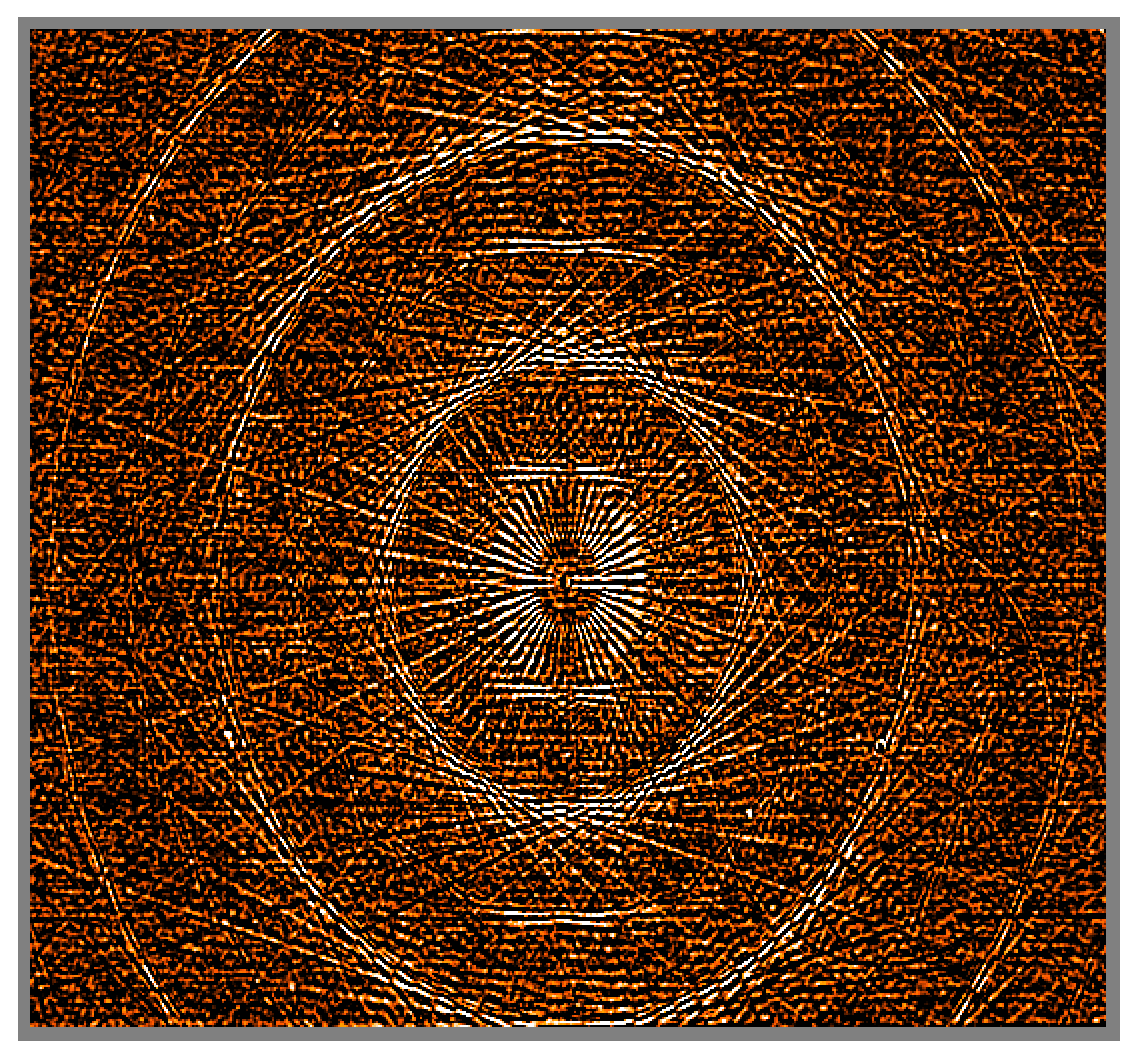
\includegraphics[width=.5\columnwidth]{B0_solution_60}%
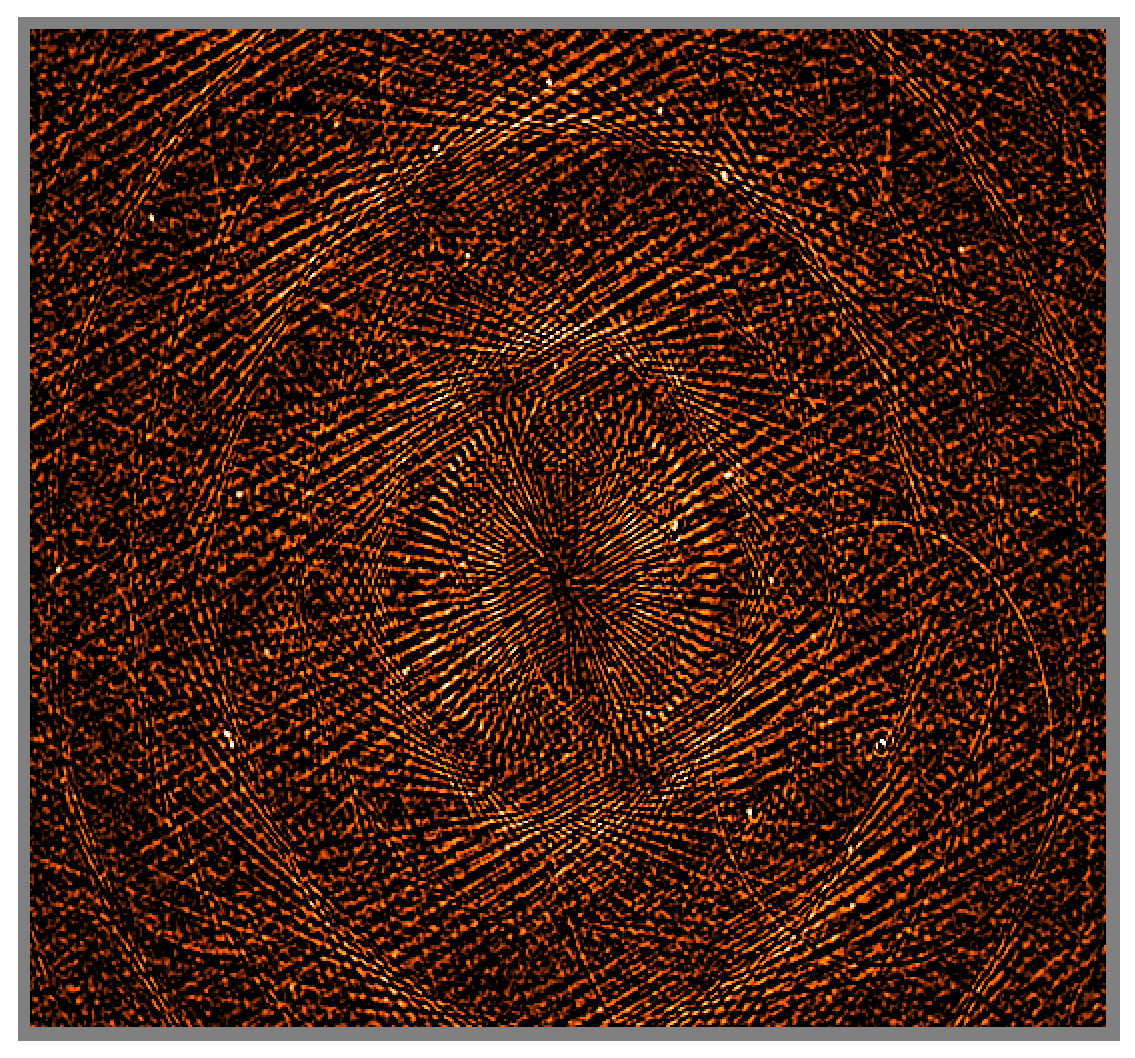
\includegraphics[width=.5\columnwidth]{B0_solution_30}\par
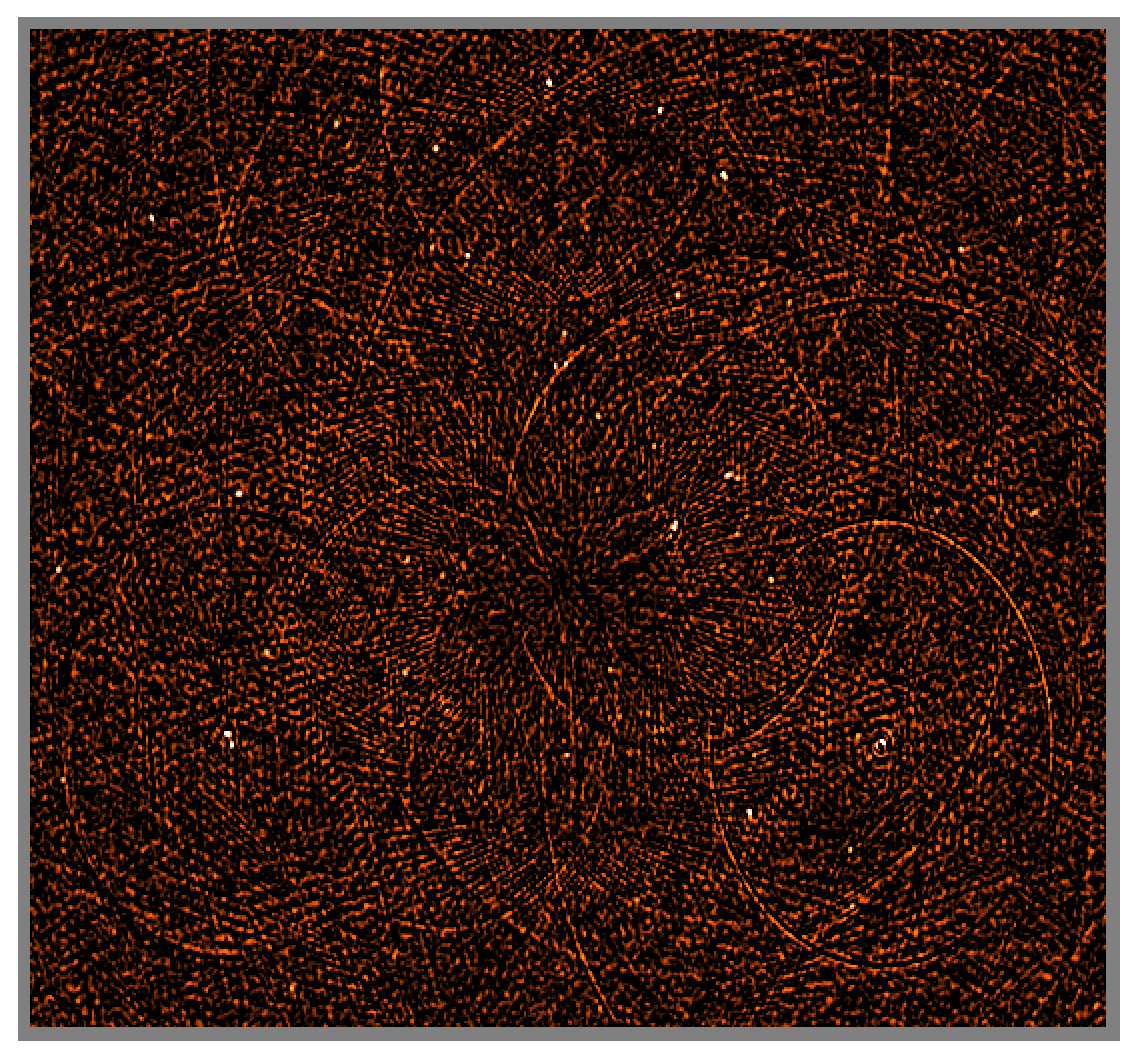
\includegraphics[width=.5\columnwidth]{B0_solution_15}%
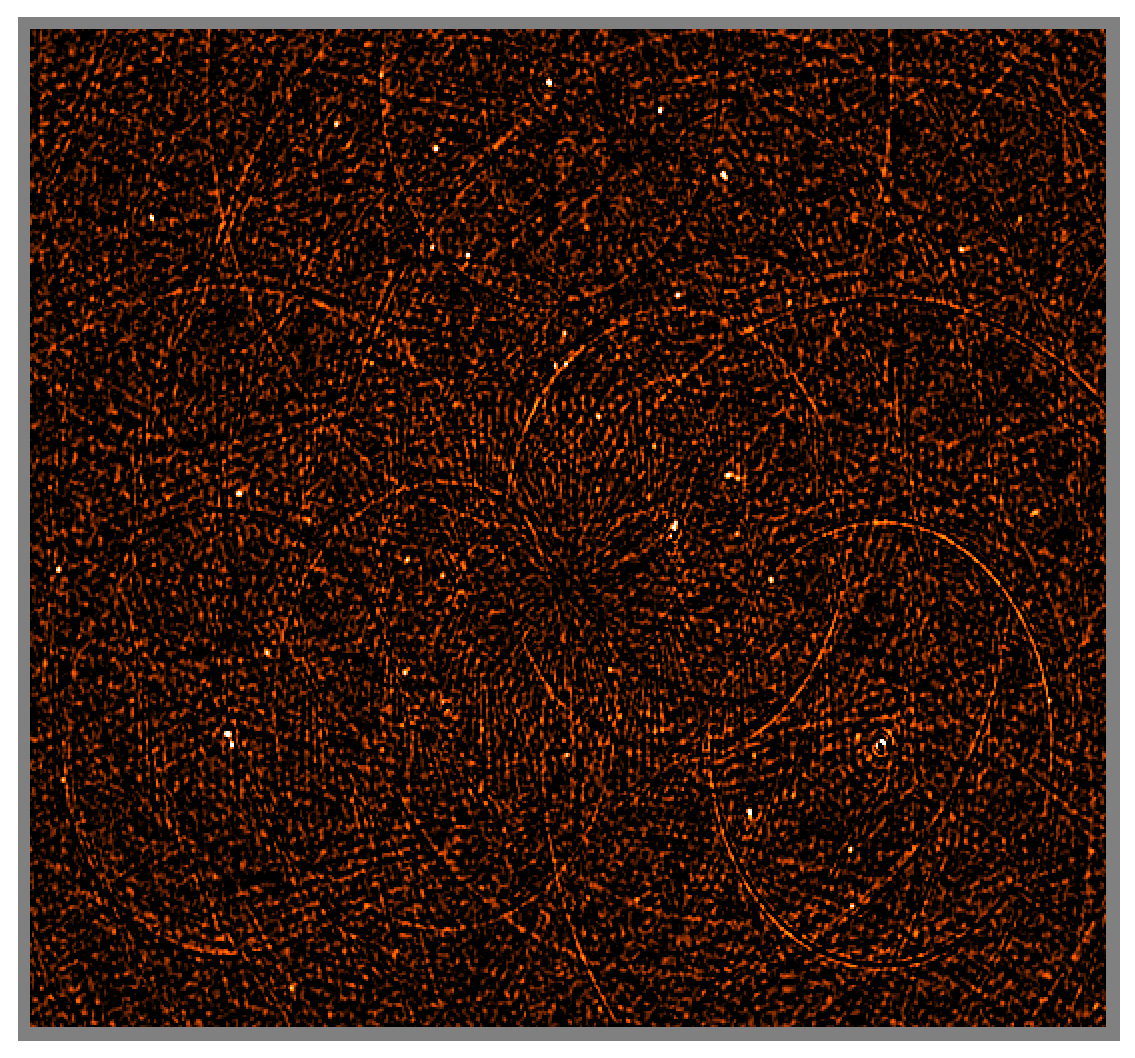
\includegraphics[width=.5\columnwidth]{B0_spline}\par
\end{centering}
\caption{\label{fig:Bsol}Single-band residual images produced via bandpass selfcal with different solution intervals for $\jones{B}{p}$: 30 minutes (upper left), 15 minutes (upper right), 7.5 minutes (lower left), and with the 7.5 minute solution smoothed using splines (lower right). Even in the best-case image, the dominant source 3C147 was not subtracted out perfectly, leaving behind DR-limiting artifacts.}
\end{figure}

The initial result of this calibration was profoundly unsatisfactory (Fig.~\ref{fig:Bsol}, upper left). The residual image was dominated by spoke-like artifacts centered on 3C147, at about 10,000:1 level (relative the flux of 3C147 itself). These spokes correspond to edges of the 30-minute solution intervals (being an E-W array, WSRT has a one-dimensional instantaneous PSF). The obvious explanation for the error is short-term bandpass instability. Decreasing the solution interval of $\jones{B}{p}$ to 15 and 7.5 minutes reduced the artifacts to levels of 50,000:1 to 100,000:1, but did not eliminate them entirely. Smoothing the 7.5 minute solution with a spline (along the time axis, per each channel independently) produced a marginal improvement (Fig.~\ref{fig:Bsol}, lower right). Subtraction artifacts are still plainly visible in the map, althought at a level not significantly above thermal noise.

At this stage I had to conclude that the WSRT bandpass exhibits some very low-level, but extremely short-term jitter, precluding a separate bandpass selfcal at extreme dynamic ranges. On the other hand, this result also shows that where a single-band dynamic range of no more than 100,000 is expected (as is the case for many other observations), bandpass selfcal provides perfectly adequate results, and can cut down on the number of solvable parameters significantly. In the meantime, for the 3C147 study I had to revert to the per-channel selfcal approach of de Bruyn.

\subsection{Per-channel selfcal}

The RIME for per-channel selfcal is just Eq.~(\ref{eq:3C147:bandpass}) without the bandpass term. It is, in fact, very similar to NEWSTAR's implicit equation (\ref{eq:newstar-rime}):\footnote{With the exception of the position of the $\coh{M}{pq}$ term, which is on the inside of Eq.~(\ref{eq:newstar-rime}), and on the outside here. For this particular dataset it makes no difference: since only the $XX$ and $YY$ correlations are used, all matrices in Eq.~(\ref{eq:newstar-rime}) are diagonal, and for diagonal matrices the ``$\ast$'' operator is equivalent to matrix multiplication, and commutes. For the full-polarization case, the two approaches are \emph{not} equivalent.}
 
\begin{equation}\label{eq:3C147:perchan}
\coh{V}{pq} = \coh{M}{pq} \ast \left ( \jones{G}{p} \left( \sum_s E_s \coh{X}{spq} E^{\herm}_s \right)  \jonesT{G}{q} \right )
\end{equation}

Per-channel selfcal is achieved by setting the solution interval of $\jones{G}{p}$ to one channel and one timeslot. The resulting single-band residual images are dominated by closure errors at a level of $\sim 100 \mu$Jy (or 1:200,000 relative to 3C147 itself); these go away after an $\coh{M}{pq}$ solution (Fig.~\ref{fig:Gsol}). These images are qualitatively very similar to those obtained by de Bruyn during his NEWSTAR calibration (which is to be expected, given the similarity of the equations).

\begin{figure}
\begin{centering}
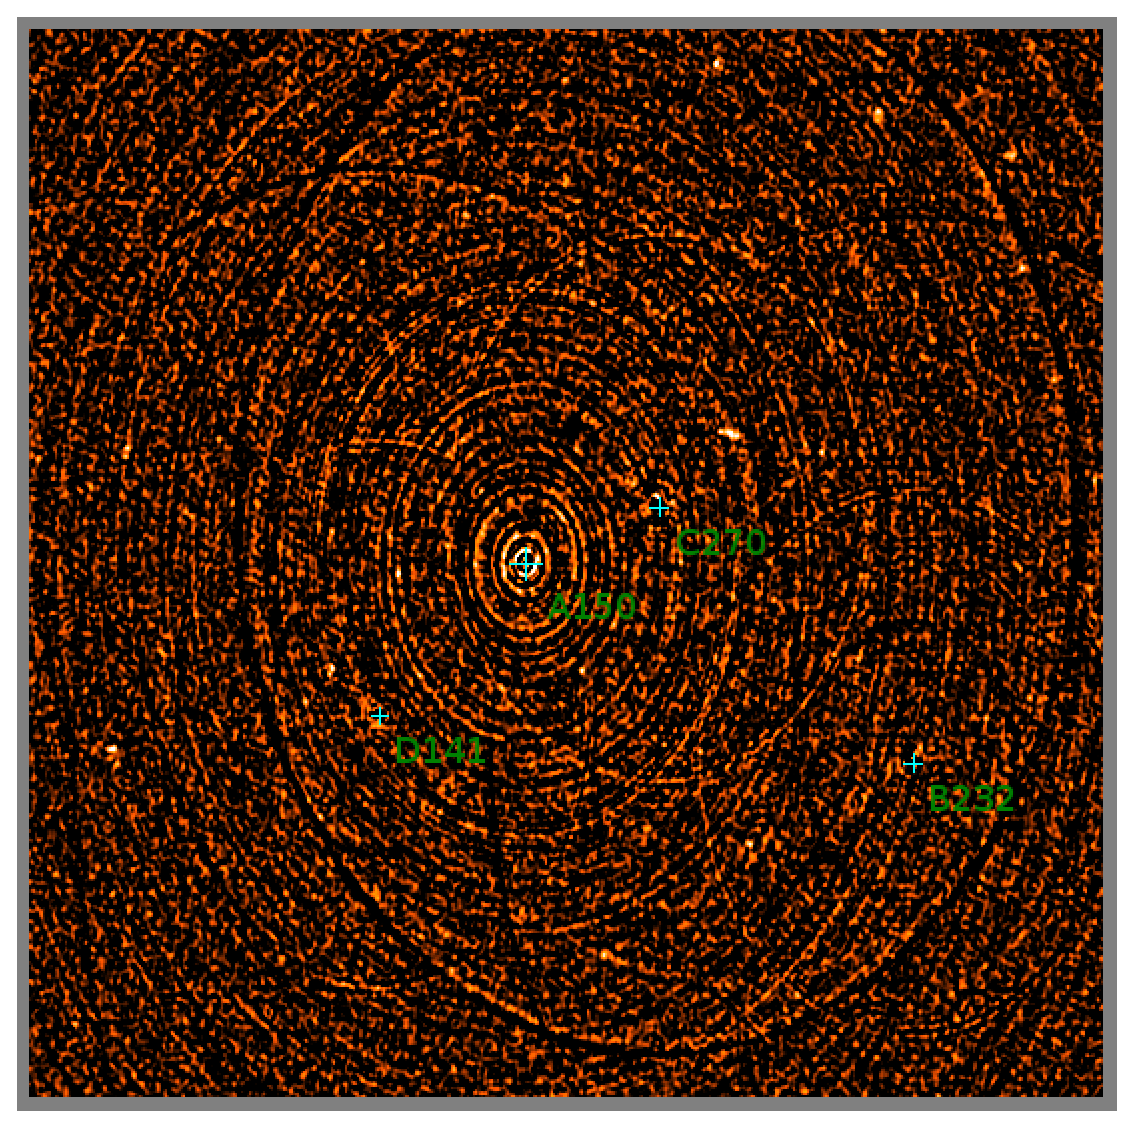
\includegraphics[width=.5\columnwidth]{G_solution}%
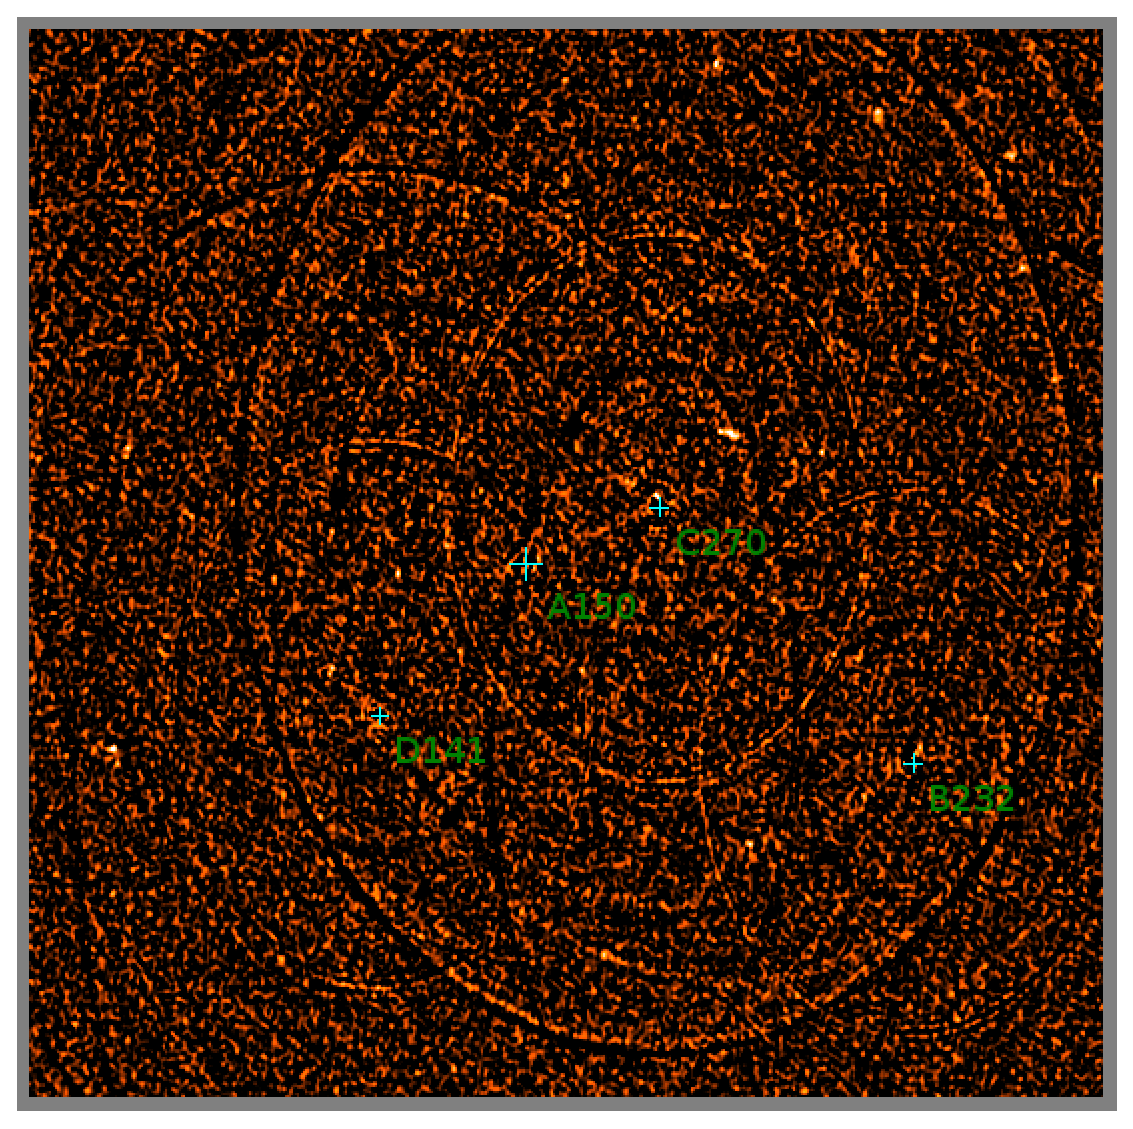
\includegraphics[width=.5\columnwidth]{IG_solution}\par
\end{centering}
\caption{\label{fig:Gsol}Single-band residual images produced via per-channel selfcal. The left image is the result of solving for $\jones{G}{p}$. It is dominated by concentric rings centered on 3C147 (designated as ``A150'' here). These are caused by closure errors, and go away once a solution for interferometer-based errors $\coh{M}{pq}$ is done (right image). The remaining artifacts are associated with off-axis sources B, C and D, and are due to DDEs. 
}
\end{figure}

The remaining artifacts in Fig.~\ref{fig:Gsol} are associated with the three next-brightest sources\footnote{The source IDs used here follow the ``COPART'' (Clustering, Order, Position Angle, Radius, Type) convention, as implemented by the Tigger sky model management tool (available with MeqTrees). A COPART source ID starts with an alphabetic designator (A, B, ... Z, aa, ab, ...) assigned to sources in order of decreasing brightness. This is already a unique identifier, and is sometimes used by itself for brevity, as in the paragraph above. A full ID also encodes approximate position relative to field center: two digits for the position angle (in units of $10\degr$), and one digit for radial distance (in units of $10\arcmin$). Optional suffixes incidate source type and clustering. Thus the full ID of source B is B232; being slightly extended, in this particular sky model it is actually represented by a cluster of six delta functions: B232, B232a, ... B232e.} in 
the field: B (42~mJy), C (52~mJy), and D (22~mJy). The furthest of these (B) is about 20$\arcmin$ away from centre. The artifacts themselves are under $50 \mu$Jy (thermal noise in one band being $\sim 30 \mu$Jy), or at a level of 1:1000 relative to the associated sources. This is why \citet{deBruyn:million} talks about an ``off-axis dynamic range'' of a 1000: while 3C147 itself (22~Jy) is subtracted without a trace (down to the thermal noise), the off-axis sources are only subtracted to a precision of about 1000. Some of the artifact structure is doubtlessly due to slightly under- or overestimated sky model fluxes (this produces regular rings matching the WSRT PSF), which can be taken care of during subsequent deconvolution. Most of it, however, is due to DDEs and does not deconvolve, producing artifacts in the final 8-band images such as the one shown in the left inset of Fig.~\ref{fig:3C147} (the inset is, in fact, a close-up of source B).

\subsection{Interferometer-based errors\label{sec:3C147:closure-errors}}

It is not clear what causes closure errors at the WSRT. Common sense suggests the analog part of the signal chain is to blame, but there is no hard evidence either way. What is evident is that high-DR images exhibit concentric ring-like artifacts such as those in the left image of Fig.~\ref{fig:Gsol}, and that these go away once a solution for an interferometer-based  multiplicative error -- the $\coh{M}{pq}$ term of Eq.~(\ref{eq:3C147:perchan}) -- is applied. A single solution per band, per the entire 12 hours (per correlation and interferometer) is sufficient. The $\coh{M}{pq}$ solutions are usually within $10^{-3}-10^{-4}$ of unity (as is the case here), but can be much higher in some observations, for reasons that remain mysterious. 

The latter fact suggests an intrinsic time variability, but solving for $\coh{M}{pq}$ on short time intervals is very dangerous. Any solution for $\coh{M}{pq}$ will also try to compensate for observed flux that is not present in the sky model. Unless the solution interval is sufficiently long, there will be unmodelled sources with a fringe rate slow enough that their vector average visibility over the solution interval will be significantly non-zero. These sources will then tend to be attenuated by the $\coh{M}{pq}$ solutions. The 3C147 observations provide a perfect example (Fig.~\ref{fig:source-suppression}). On the left is an 8-band residual image with a 12 hour $\coh{M}{pq}$ solution; on the right is one with a 30 minute solution. Model sources are indicated by crosses. Attenuation of unmodelled sources towards phase centre is clearly visible in the right image. 

\begin{figure}
\begin{centering}
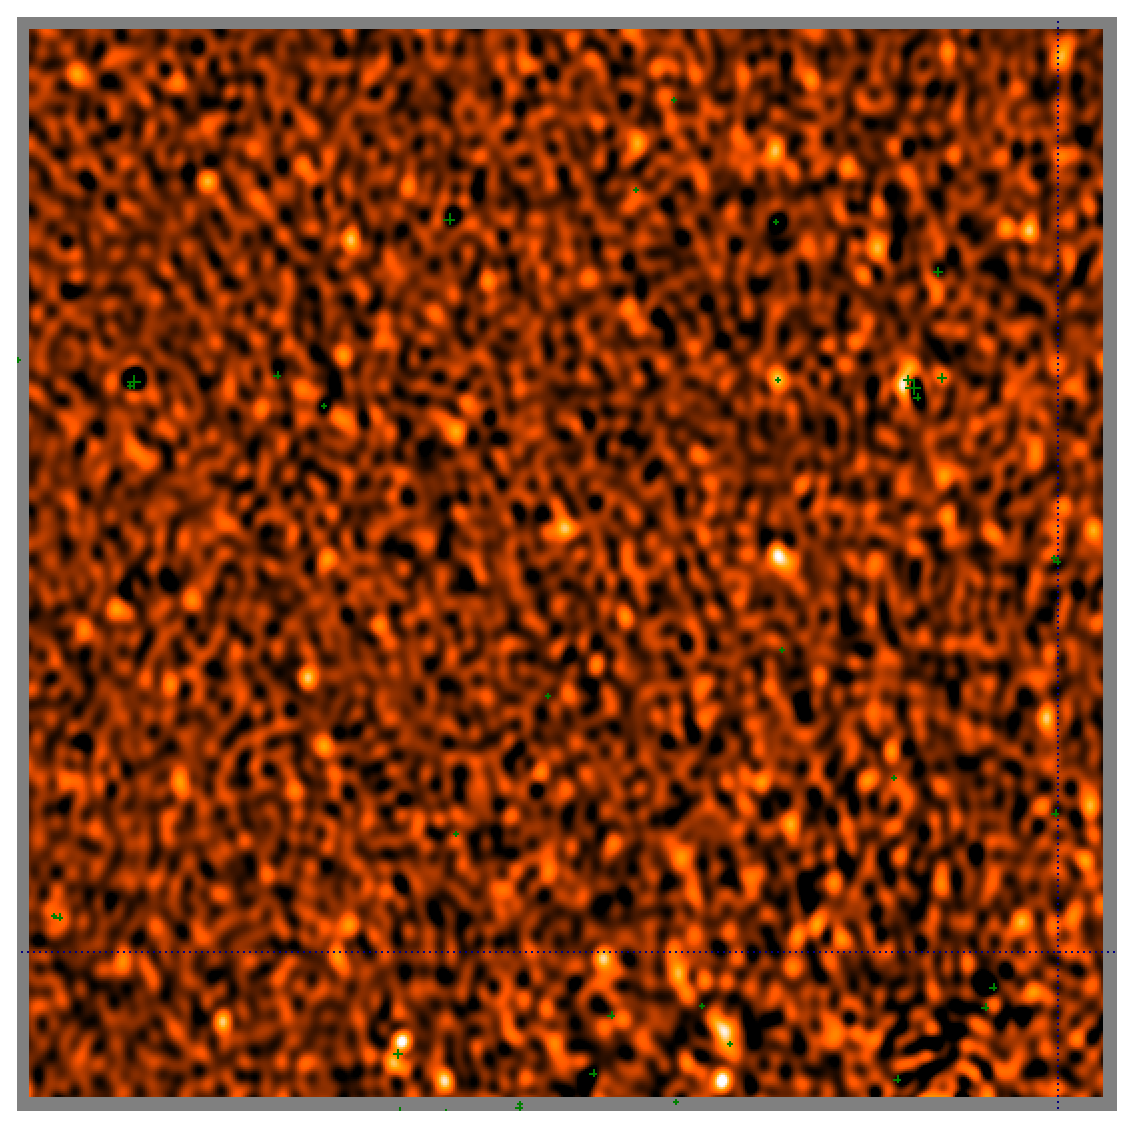
\includegraphics[width=.5\columnwidth]{IG_12h}%
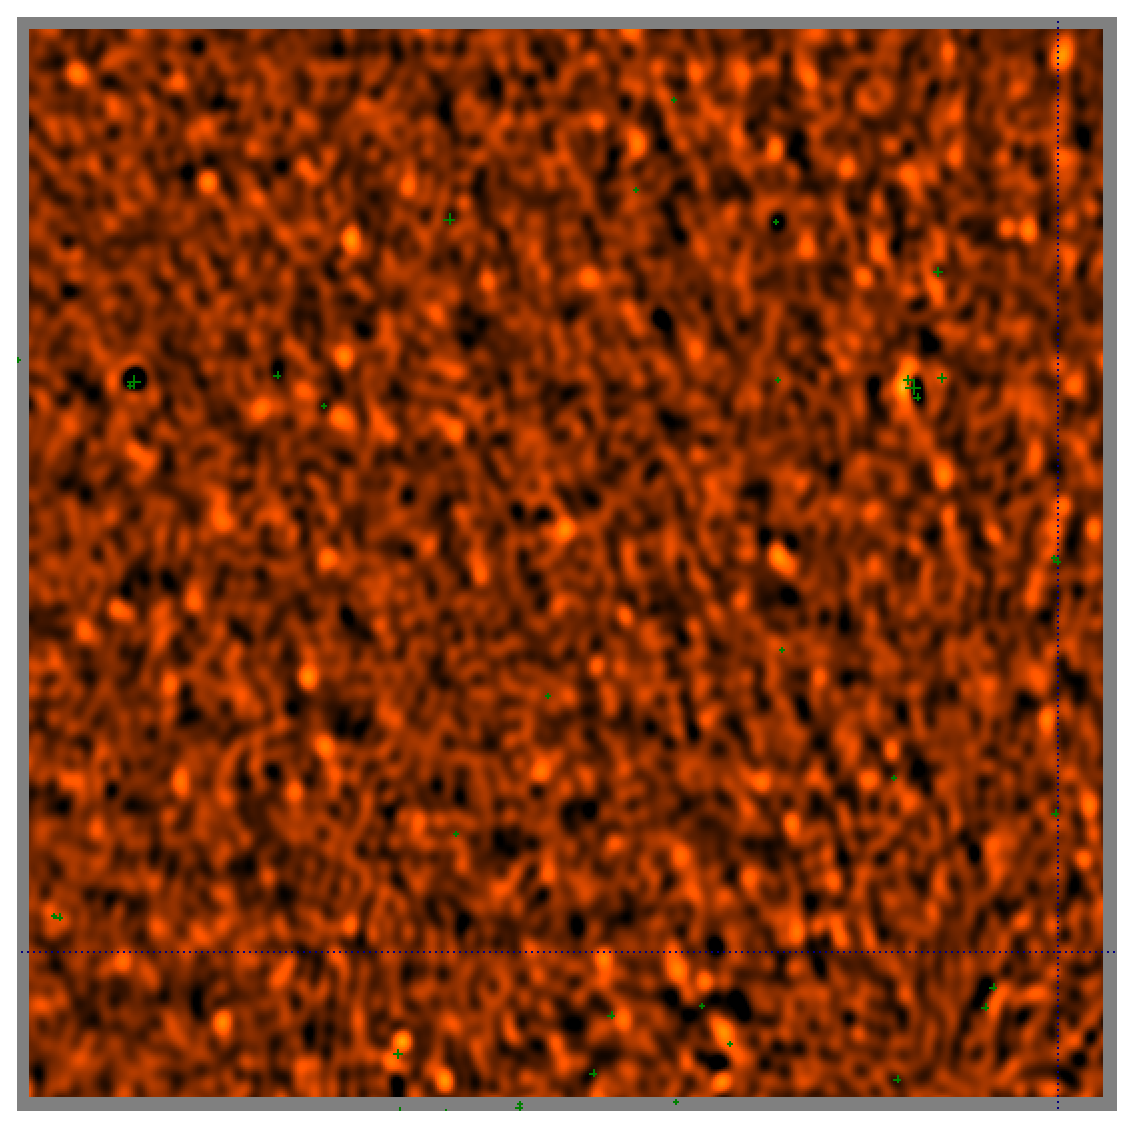
\includegraphics[width=.5\columnwidth]{IG_30m}\par
\end{centering}
\caption{\label{fig:source-suppression}Source suppression through interferometer-based error solutions. On the left is a deconvolved 8-band residual image of the center of the field, with 12 hour solutions for $\coh{M}{pq}$. On the right is the same image with 30 minute solutions. The positions of (subtracted) model sources are indicated by crosses. Suppression of unmodelled sources is evident in the right image.
}
\end{figure}


This implies that closure errors cannot be reliably solved for on observations shorter than 12 hours, unless a ``complete'' (i.e. down to the noise) sky model of the center of the field is available.

\subsection{Pointing selfcal\label{sec:3C147:pointing}}

Since the main cause of artifacts in WSRT images is commonly considered to be pointing error (see Sect.~\ref{sec:pointing}), I decided to implement a version of the pointing selfcal algorithm suggested by \citet{SB:pointing}. This proved to be a straightforward exercise in MeqTrees, since only a small modification of the RIME of Eq.~(\ref{eq:3C147:perchan}) was required: 

\begin{equation}\label{eq:3C147:pointing}
\coh{V}{pq} = \coh{M}{pq} \ast \left ( \jones{G}{p} \left( \sum_s E_{sp} \coh{X}{spq} E^{\herm}_{sq} \right) \jonesT{G}{q} \right )
\end{equation}

Instead of a per-source beam gain $E_s=E(l_s,m_s)$ (where $E(l,m)$ is the $\cos^3$ approximation given by Sect.~\ref{sec:EJones:wsrt}), which I had been using in the previous equations, here I used a per-antenna, per-source beam gain $E_{sp}$, defined as follows:

\begin{equation}\label{eq:3C147:offset-beam}
E_{sp} = E(l_s+\delta l_p,m_s+\delta m_p)
\end{equation}

Per-antenna pointing offsets $\delta l_p,\delta m_p$ were then treated as solvable parameters. 

The results of this proved inconclusive. Even though the solution converged to some physically-sensible offsets (on the order of arcmin), no tangible reduction of artifacts was observed in residual images. This could be due to a number of reasons:

\begin{enumerate}
\item The $\cos^3$ approximation is not good enough -- unlikely, as it has been independently verified at least for the core of the main lobe, which the sources in question sources are well within.
\item With only a few sources sufficiently bright to exhibit DDEs, we simply don't have enough constraints for a pointing solution on this field.
\item The model fluxes/positions for the sources in question are not sufficiently accurate.
\item The dominant DDE affecting this observation is not pointing error. This will be elaborated on further in Sect.~\ref{sec:de-analysis}. 
\item There is something wrong with my implementation of pointing selfcal, especially since the figures in Sect.~\ref{sec:de-analysis} suggest that mispointings \emph{are} detectable.
\end{enumerate}

Trying to get a better grip on the problem, I eventually settled on a ``controlled experiment'':
locating a field containing multiple bright off-axis sources, and observing it with deliberately exaggerated mispointings, to see if these can be more readily recovered from the data. This experiment became known as the ``QMC Project'' (in honour of the long-defunct Quality Monitoring Committee of WSRT), and was successfully carried out. The results of this are still being processed, and will be presented in a follow-up paper. 
In the meantime, I had to look for alternative approaches to DDEs in the 3C147 field.

\subsection{Differential gains: the ``flyswatter''\label{sec:diffgains}}

In the spirit of ``phenomenological'' equations discussed in Sect.~\ref{sec:phenomenological}, I decided to introduce a {\em differential gain} Jones ($\Delta E$-Jones) into my form of the RIME:

\begin{equation}\label{eq:3C147:de}
\coh{V}{pq} = \coh{M}{pq} \ast \left ( \jones{G}{p} \left( \sum_s \Delta\jones{E}{sp} E_s \coh{X}{spq} E^{\herm}_s \Delta\jonesT{E}{sq} \right)  \jonesT{G}{q} \right )
\end{equation}

The $\Delta\jones{E}{sp}$ term is meant to subsume {\bf all} DDEs associated with source $s$ and antenna $p$ (with the exception of the nominal primary beam gain, which is already represented by $E_s$). Solving for this term requires some caution, lest too many DoF's be introduced into the equation. I approached this as follows:

\begin{itemize}
\item $\Delta\jones{E}{}$ was fixed at unity for all sources except B, C, and D;
\item For B, C and D, $\Delta\jones{E}{}$ was set to a diagonal matrix with solvable complex elements.
\item The solution intervals for the $\Delta\jones{E}{}$ elements were set to one solution per 30 minutes, per entire band (and per source, antenna, receptor).
\end{itemize}

\begin{figure}
\begin{centering}
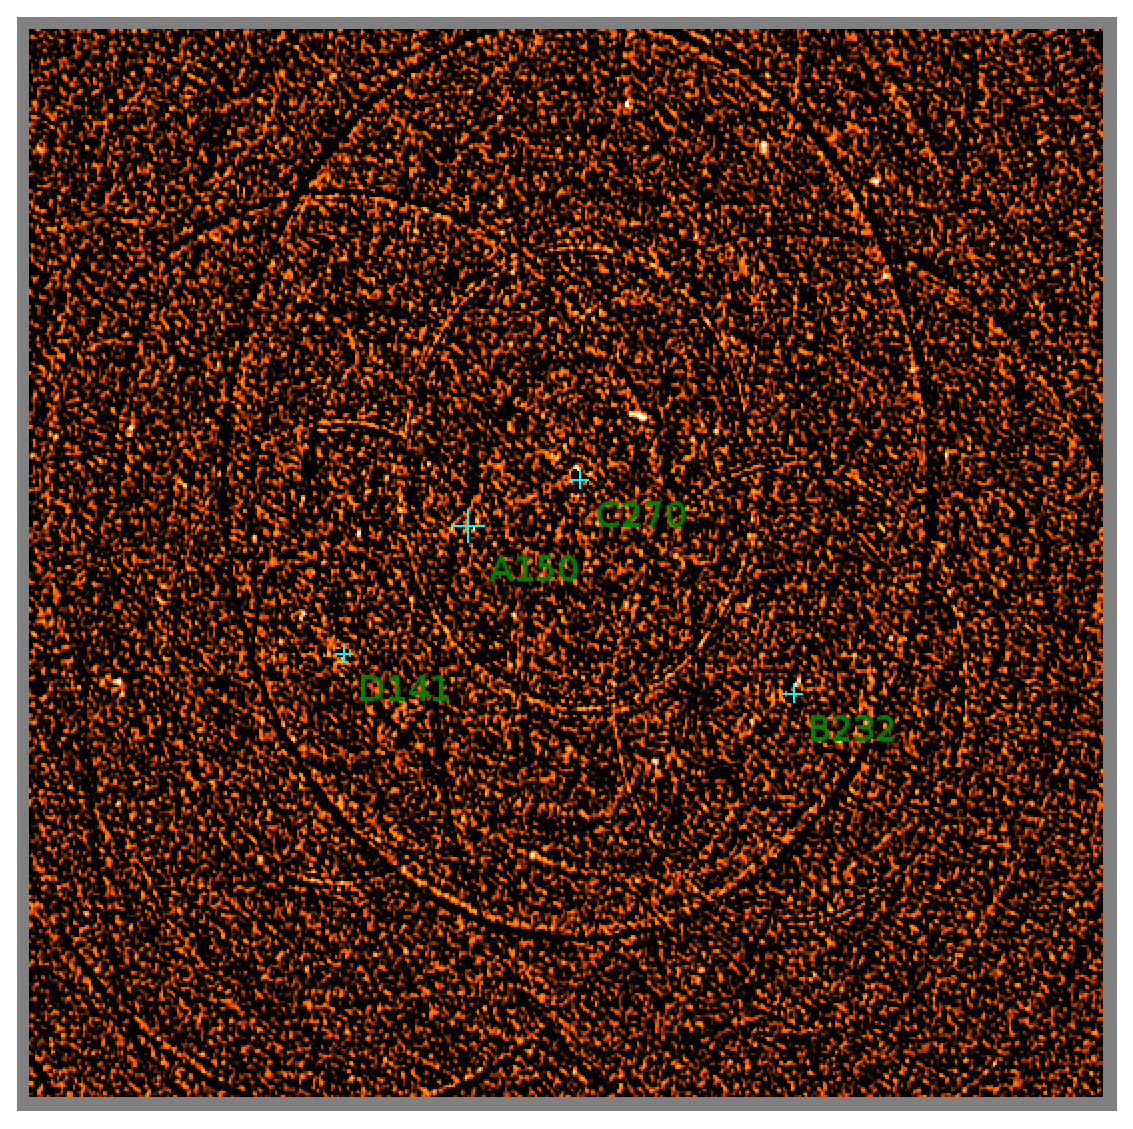
\includegraphics[width=.5\columnwidth]{before_dE}%
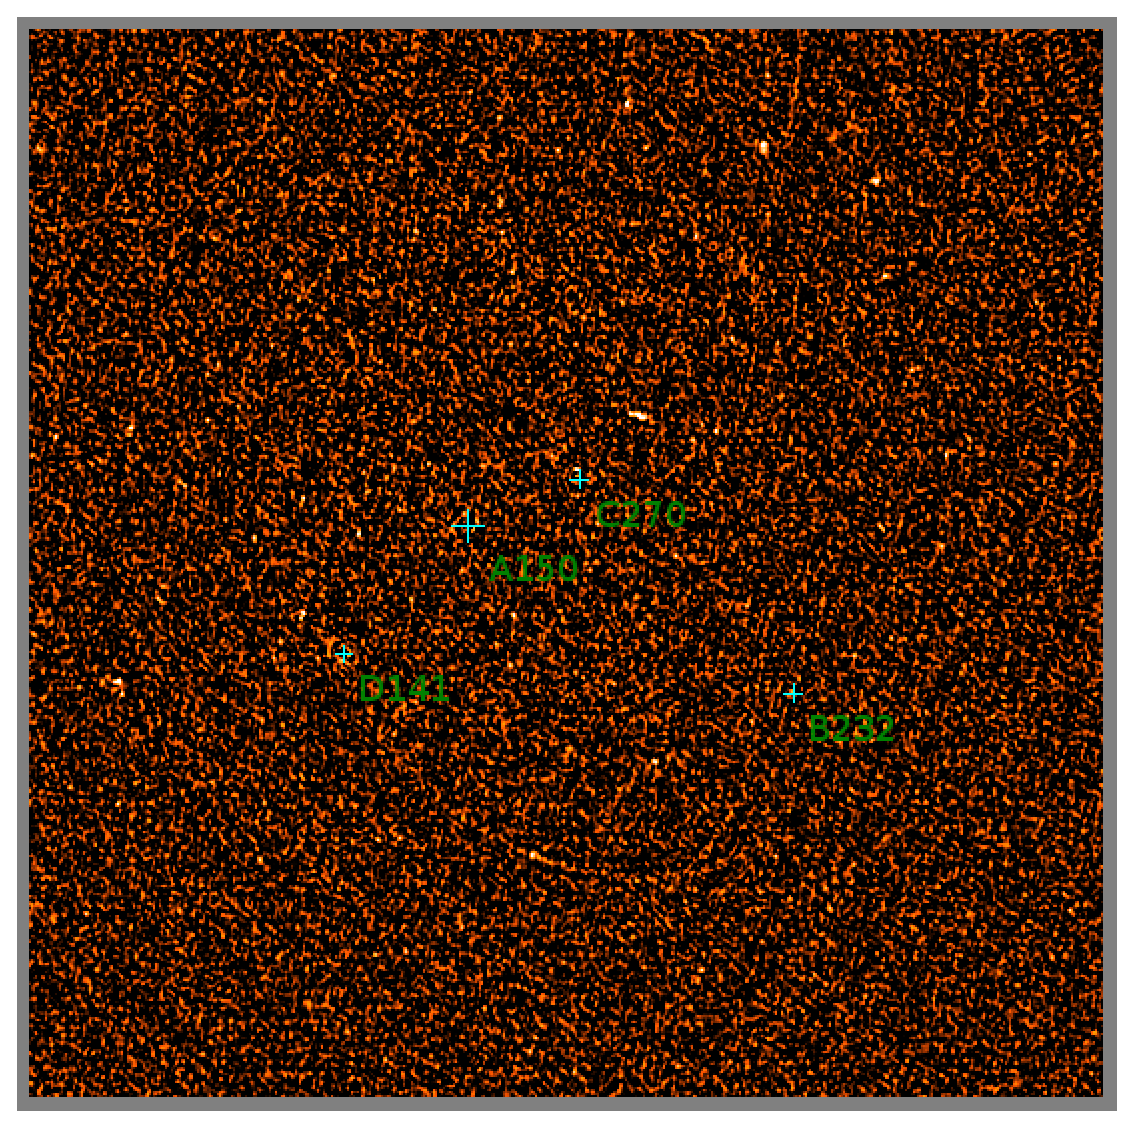
\includegraphics[width=.5\columnwidth]{after_dE}\par
\end{centering}
\caption{\label{fig:dEsol}Results if the flyswatter. On the left is a single-band residual image after  $\jones{G}{p}$ and $\coh{M}{pq}$ solutions only. On the right is the same image with differential gain solutions for sources B, C, and D.}
\end{figure}

Figure~\ref{fig:dEsol} shows the effect of $\Delta\jones{E}{}$ solutions. All artifacts associated with sources B, C and D disappeared completely, to the point where artifacts around fainter sources became just about visible. These were later eliminated once $\Delta\jones{E}{}$ solutions were enabled for those sources. In fact, any source to which a solvable $\Delta\jones{E}{}$ term was assigned promptly vanished from the residual maps, hence my name for the differential gains approach: the ``flyswatter'' algorithm. 

Once 8-band residual images were created, the increased sensitivity made it apparent that four more sources were exhibiting a small amount of DDEs. A more in-depth look at the sky model also showed that all seven sources were in fact slightly extended; the NEWSTAR model represented each by a tight cluster of point sources. Since all ``sources'' in such a cluster are subject to the same DDE, it seemed sensible to make sure the same $\Delta\jones{E}{sp}$ term was applied to all of them. This was easily done using Tigger, a sky model manager/viewer tool included with MeqTrees. Tigger automatically detects source clusters and assigns source identifiers appropriately (e.g. B232, B232a, ...  B232e) It was then a simple matter to tell the Calico framework to use the \emph{same} $\Delta\jones{E}{s_0 p}$ term for all sources $s$ associated with cluster $s_0$. 

%plot-de-solutions.py --circle-ampl -o eps --portrait --borders 0.05,0.98,0.05,0.98 --title-fontsize 0 -r o2003.cache --circle-minsize=0 --circle-maxsize=0 --label-fontsize=16 --names-only --radius 70
\begin{figure}
\begin{minipage}[c]{.45\columnwidth}
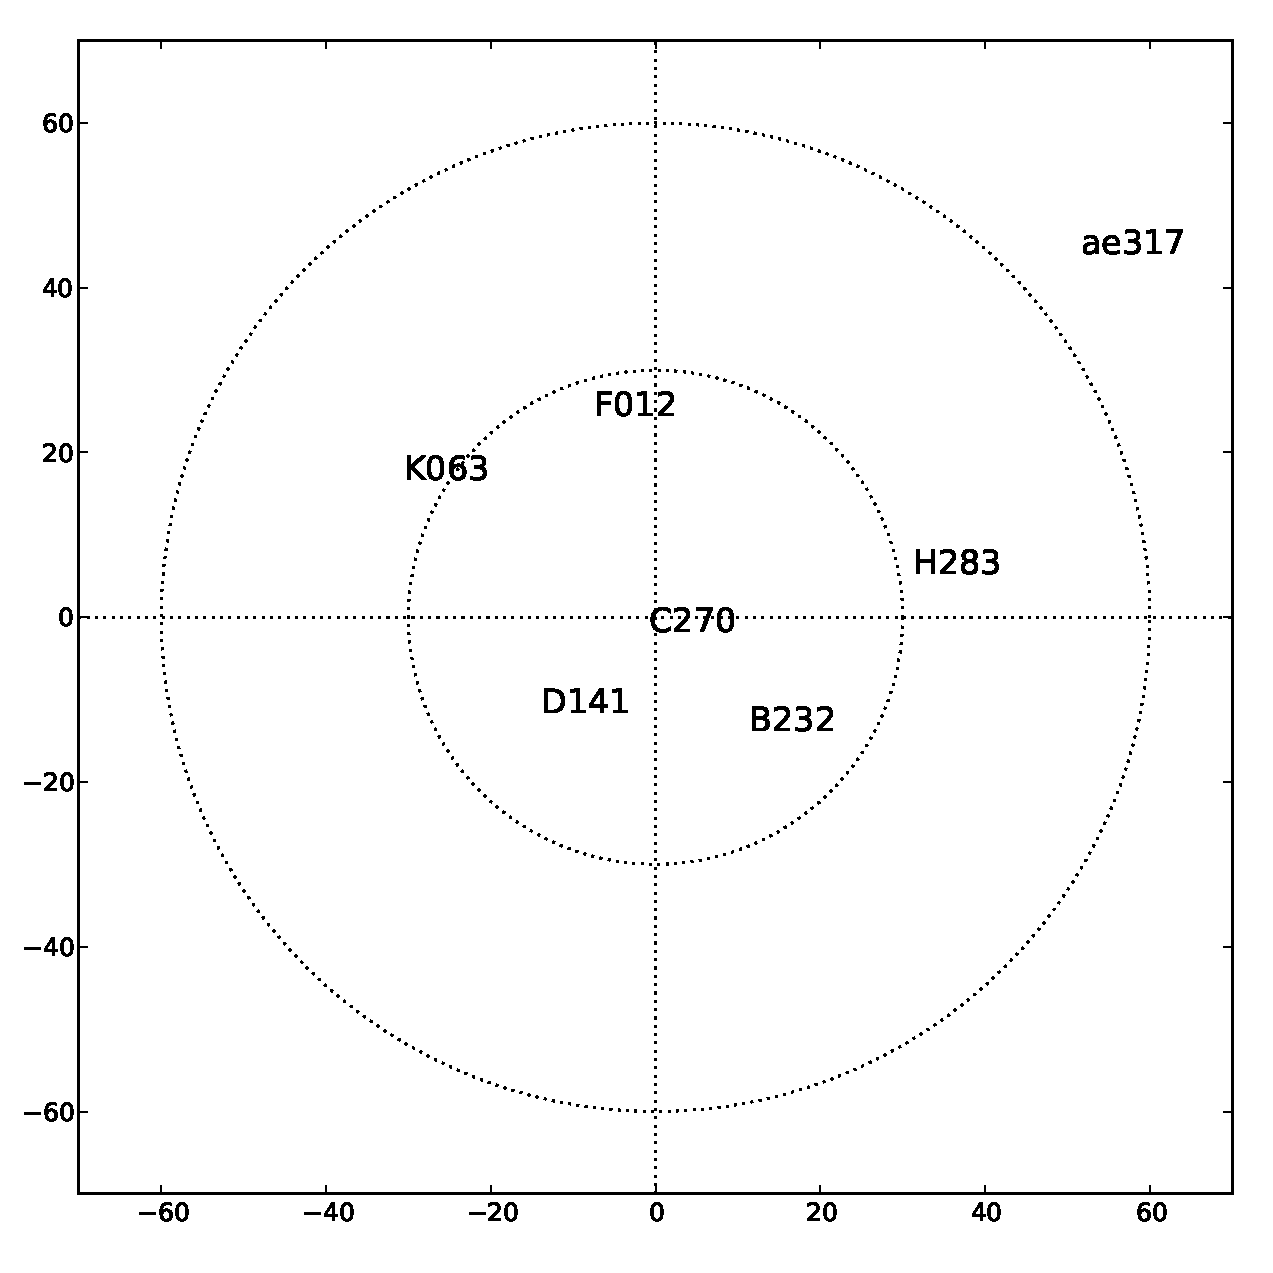
\includegraphics[width=\textwidth]{source_plot}
\end{minipage}\hfill\begin{minipage}[c]{.5\columnwidth}
\begin{tabular}{lr@{ }lr@{.}l}
\hline
\hline
ID & \multicolumn{2}{c}{position} & \multicolumn{2}{c}{total flux} \\
% \multicolumn{2}{c}{source ID} & \multicolumn{2}{c}{position} & \multicolumn{2}{c}{total flux} \\
\hline
B232  & 20' & SW & 42 & 3 mJy\\
C270  &  4' & W  & 51 & 8 mJy\\
D141  & 14' & SE & 21 & 8 mJy\\
F012  & 25' & N  & 12 & 3 mJy \\
H283  & 37' & W  &  9 & 4 mJy \\
K063  & 31' & NE &  8 & 2 mJy \\
ae317 & 74' & NW &  2 & 2 mJy \\
%  B232 & (NEWS1000)   & 20' & SW & 42 & 3 mJy\\
%  C270 & (NEWS7)      &  4' & W  & 51 & 8 mJy\\
%  D141 & (NEWS9)      & 14' & SE & 21 & 8 mJy\\
%  F012 & (NEWS1009)   & 25' & N  & 12 & 3 mJy \\
%  H283 & (NEWS1037)   & 37' & W  &  9 & 4 mJy \\
%  K063 & (NEWS1041)   & 31' & NE &  8 & 2 mJy \\
%  ae317 & (NEWS3159)  & 74' & NW &  2 & 2 mJy \\
\hline
\end{tabular}
\end{minipage}

\caption{\label{fig:source-plot}Positions (relative to nominal pointing center) and aggregate fluxes (apparent) of the seven off-axis source clusters for which $\Delta\jones{E}{}$ solutions were obtained. Circles are at a radius of $30\arcmin$ and $1\degr$. For reference, the FWHM of the WSRT voltage beam is $\sim50\arcmin$ at 1.4~GHz.}
\end{figure}

The seven source clusters for which differential gain solutions were eventually obtained are summarized in Fig.~\ref{fig:source-plot}. Two of them are somewhat noteworthy. Source {\bf C270} is very close to center, and therefore shouldn't be affected by DDEs as much as the other sources. It is, however, a complicated and highly polarized source, so perhaps the artifacts it exhibits after regular selfcal are primarily due to sky model inaccuracies, which the $\Delta\jones{E}{}$ solutions absorb (see discussion in Sect.~\ref{sec:de-analysis-model}). Source {\bf ae317} is almost the opposite: it is very faint, but far enough off-axis to be in a sidelobe of the primary beam, and so subject to especially severe DDEs.

\subsection{The showcase result} 

The ultimate result of my calibration of the 2003 observation is shown in Fig.~\ref{fig:3C147}. This image is a true showcase for the differential gains approach. The precise steps leading to this image were as follows:

\begin{enumerate}

\item Each of the 8 bands was independently calibrated using per-channel selfcal, interferometer-based errors, and $\Delta\jones{E}{}$ solutions on seven source clusters, as described above. Corrected residuals were generated.

\item The residuals for all 8 bands were imaged together (in MFS mode) to produce a single residual image. This revealed a large number of fainter sources not visible in the per-band maps.

\item The 8-band image was deconvolved using Cotton-Schwab CLEAN \citep{Schwab:csclean}.

\item The sky model was added back into the deconvolved image, using a Gaussian restoring beam.

\end{enumerate}

The resulting image is completely artifact-free. Presumably, all other sources in the field are too faint to exhibit any DDE-related artifacts. With a dynamic range of 1,600,000:1, this image is the deepest and cleanest single-synthesis radio map in the world to date. 

\subsection{Flyswatter limitations\label{sec:dE-limitations}}

While it can help produce spectacular images, the flyswatter has some serious caveats and drawbacks that need to be explored. First of all, it is a brute-force approach, in the sense that it squashes all effects into a single $\Delta\jones{E}{}$ term. This includes inaccuracies in the sky model! Indeed, any missing source flux or error in source position can be accomodated with a suitable $\Delta\jones{E}{}$. Even unmodelled source structure can ``leak'' into differential gain solutions (Sect.~\ref{sec:de-analysis-model}). Thus, differential gains are good for subtracting sources, but at the cost of mashing up information on the source per se. (One does not use a flyswatter to probe a fly's anatomy!)

Secondly, solvable differential gains can lead to a proliferation of DoF's. Per-channel selfcal has $N_\mathrm{ant}$ unknowns per $\frac{N_\mathrm{ant}(N_\mathrm{ant}-1)}{2}$ measurements, or $\frac{2}{N_\mathrm{ant}-1}$ unknowns per measurement; differential gains add $\frac{2N_\mathrm{src}}{(N_\mathrm{ant}-1)N_\mathrm{time}N_\mathrm{freq}}$ unknowns per measurement, where $N_\mathrm{time}$ and $N_\mathrm{freq}$ are the sizes of the solution interval for $\Delta\jones{E}{}$. This ratio remains favourable for small $N_\mathrm{src}$ and large $N_\mathrm{time}$ and/or $N_\mathrm{freq}$ (as is the case for my 3C147 reduction), but one must be careful.

The third caveat is processing cost. While usually not as expensive in terms of I/O or CPU as peeling (which, in addition to the solutions themselves, requires repeated subtraction and phase shifting steps), the flyswatter is not free. Every source with a differential gain solution adds $4N_\mathrm{ant}$ unknowns (assuming a diagonal complex $\Delta\jones{E}{sp}$ term, hence 4 real values per matrix) to the equations. As the number of unknowns ($N_\mathrm{unk}=4N_\mathrm{ant}N_\mathrm{src}$) grows, inversion of the normal matrix within the least-squares solver becomes a CPU bottleneck, since it scales as $O(N_\mathrm{unk}^3)$. This makes it impractical to solve for $\Delta\jones{E}{}$'s for more than a handful\footnote{The precise meaning of a ``handful'' here depends on additional factors such as $N_\mathrm{ant}$, size of solution intervals, etc. In effect, these factors influence the constant of the overall cubic scaling law.} of sources at a time. 

One way to mitigate the solver bottleneck is to decompose the $\Delta\jones{E}{sp}$'s into nearly-orthogonal sets of unknowns. For example, we can treat the set of $\Delta\jones{E}{sp}$'s associated with one source $s$ as independent from all other sources. The $(4N_\mathrm{ant}N_\mathrm{src})^2$ normal matrix inside the solver then becomes block-diagonal, composed of $N_\mathrm{src}$ blocks of size $(4N_\mathrm{ant})^2$. Inversion of this matrix then scales as $O(N_\mathrm{src})O(N_\mathrm{ant}^3)$. This scheme was tested in MeqTrees, and it was found that the trade-off is slower convergence, requiring more iterations. For large numbers of sources, however, this becomes very favourable.

\section{Analysis of differential gain solutions\label{sec:de-analysis}}

It is time to see whether any useful information can be gleaned from the differential gains solutions themselves. As a result of the reduction, I had obtained: per each source direction (7 of these: see Fig.~\ref{fig:source-plot}), per each antenna (14), per each band (8), per 30-minute interval (24 of these in a 12-hour synthesis), two complex numbers representing the apparent differential gain of the X and Y dipole (``differential'' being relative to the gain in the direction of 3C147 -- almost at the center of the field -- which had been taken care of by regular selfcal).

I then adopted the following approach. Given the relatively low fractional bandwidth, I didn't expect much variation with frequency in $\Delta\jones{E}{}$. I therefore treated each set of 8 per-band solutions as independent samples of the same variable. The mean of the 8 samples was used as an estimator of variable, and the standard deviation of the 8 samples as an estimator of the error (i.e. the error bar).

Since it quickly became apparent that the $\Delta\jones{E}{}$ solutions were exhibiting some very interesting behaviour, I applied exactly the same procedure to the 2006 observations, so that comparisons could be made. The plots below show the results from both observations. 

%% first form to init cache
% plot-de-solutions.py --ampl --phase -o eps -r --portrait --title-fontsize 0 -W 290 -H 100 --borders 0.02,1.02,0.01,1.08 MS/3C*/dE* --output-prefix o2003 -c o2003 --axis-fontsize 8
% plot-de-solutions.py --ampl --phase -o eps -r --portrait --title-fontsize 0 -W 290 -H 100 --borders 0.02,1.02,0.01,1.08 MS/m30*/dE* --output-prefix o2006 -c o2006 --axis-fontsize 8
%% second form to reuse cache
% for t in o2003 o2006; do plot-de-solutions.py --ampl --phase -o eps -r --portrait --title-fontsize 0 --axis-fontsize 8 -W 290 -H 100 --borders 0.02,1.02,0.01,1.08 $t.cache --output-prefix $t; done
\begin{figure*}
\sidecaption
\parbox[b]{12cm}{
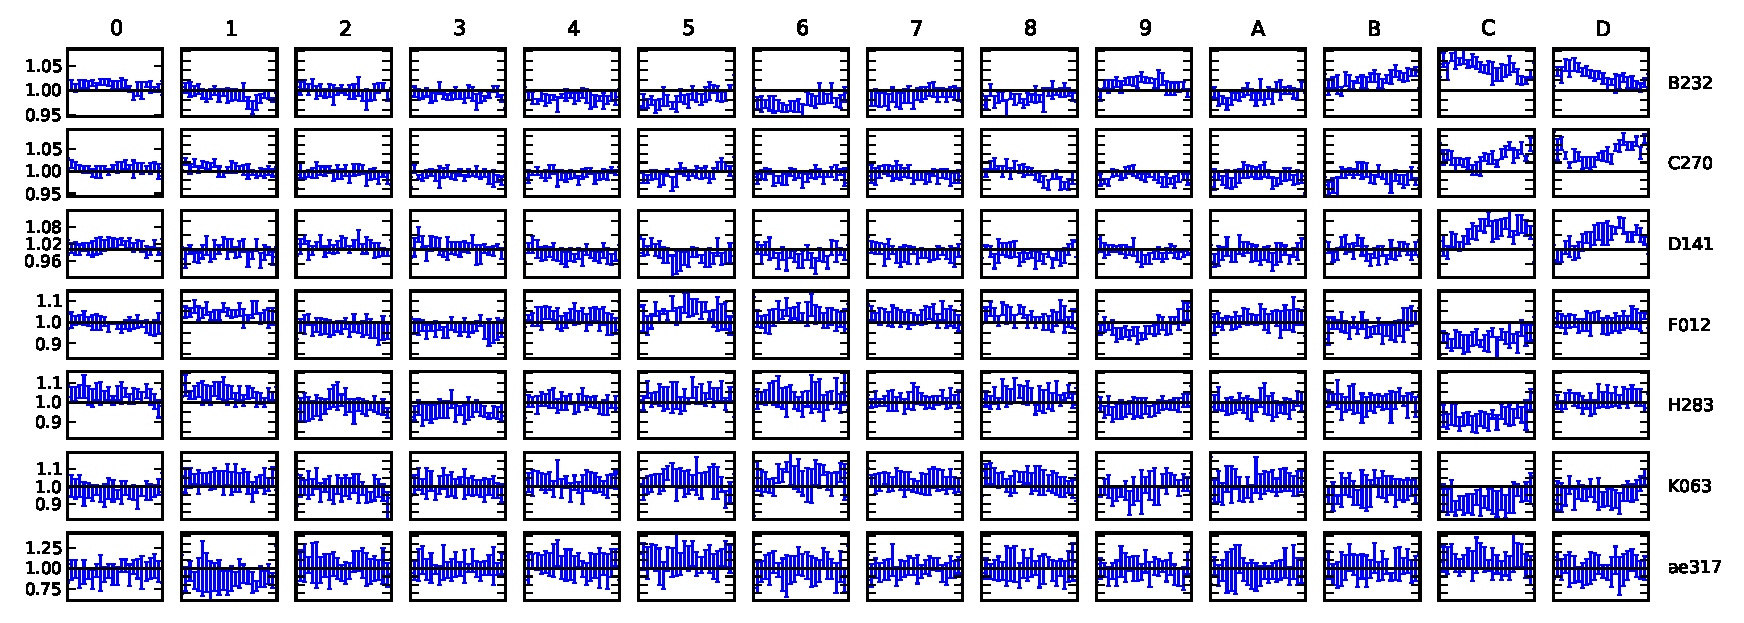
\includegraphics[width=12cm]{o2003_dE_mean} \\
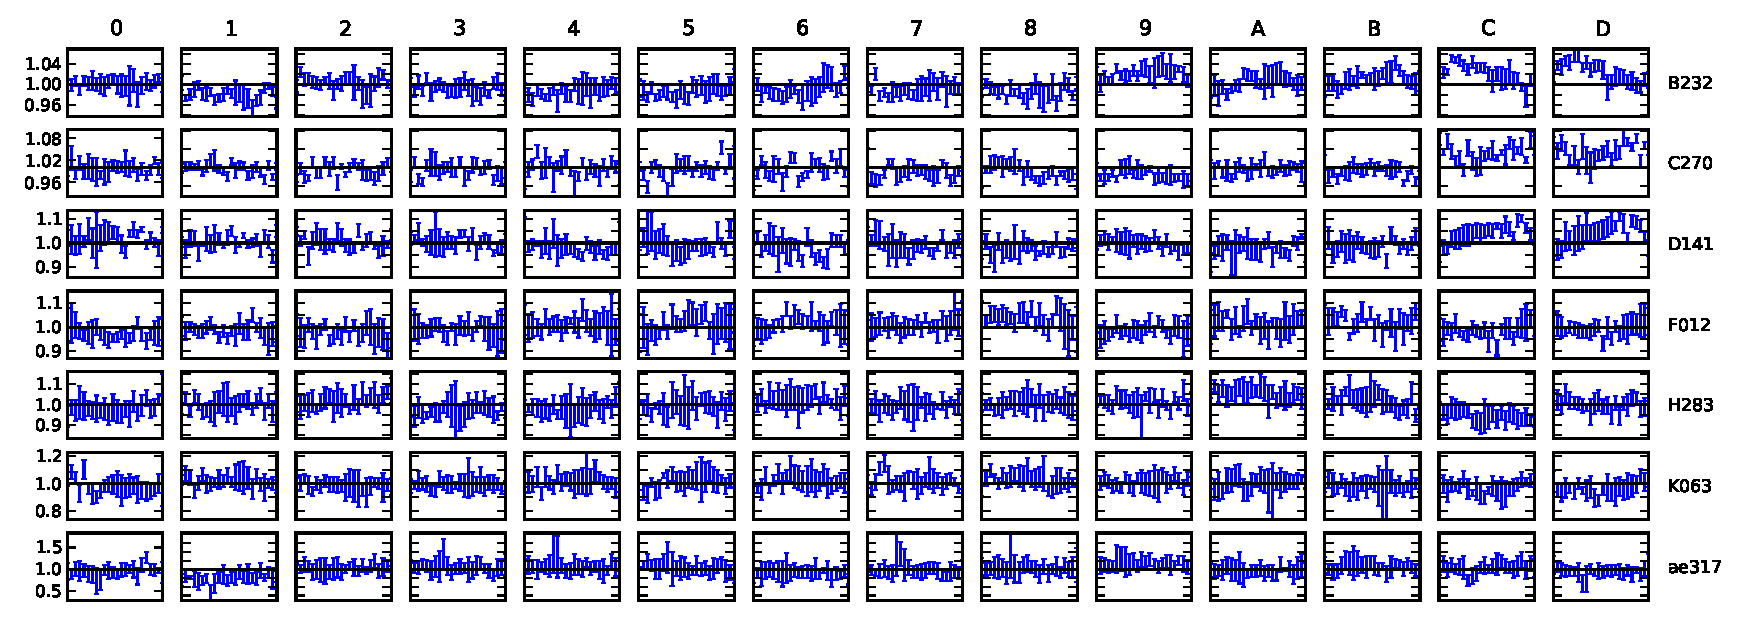
\includegraphics[width=12cm]{o2006_dE_mean}
}
\caption{\label{fig:dEampl}Differential gain-amplitudes ($||\Delta\jones{E}{}||$) as a function of time for the 2003 (top) and 2006 (bottom) observations. Rows correspond to sources, columns to antennas. The vertical plot scale is fixed within each row, but differs from row to row. Horizontal lines indicate the $||\Delta\jones{E}{}||=1$ level.}
\end{figure*}

\begin{figure*}
\sidecaption
\parbox[b]{12cm}{
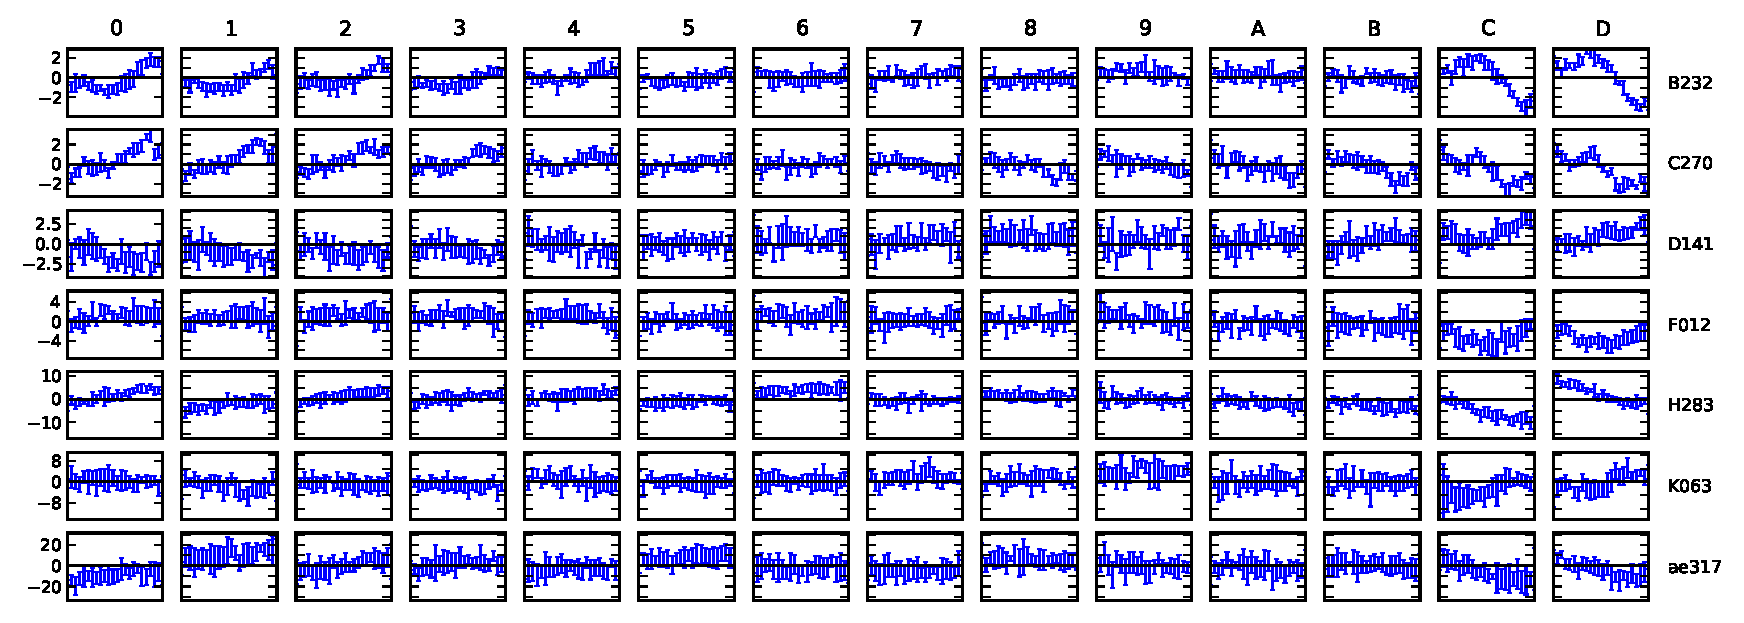
\includegraphics[width=12cm]{o2003_dEphase_mean}
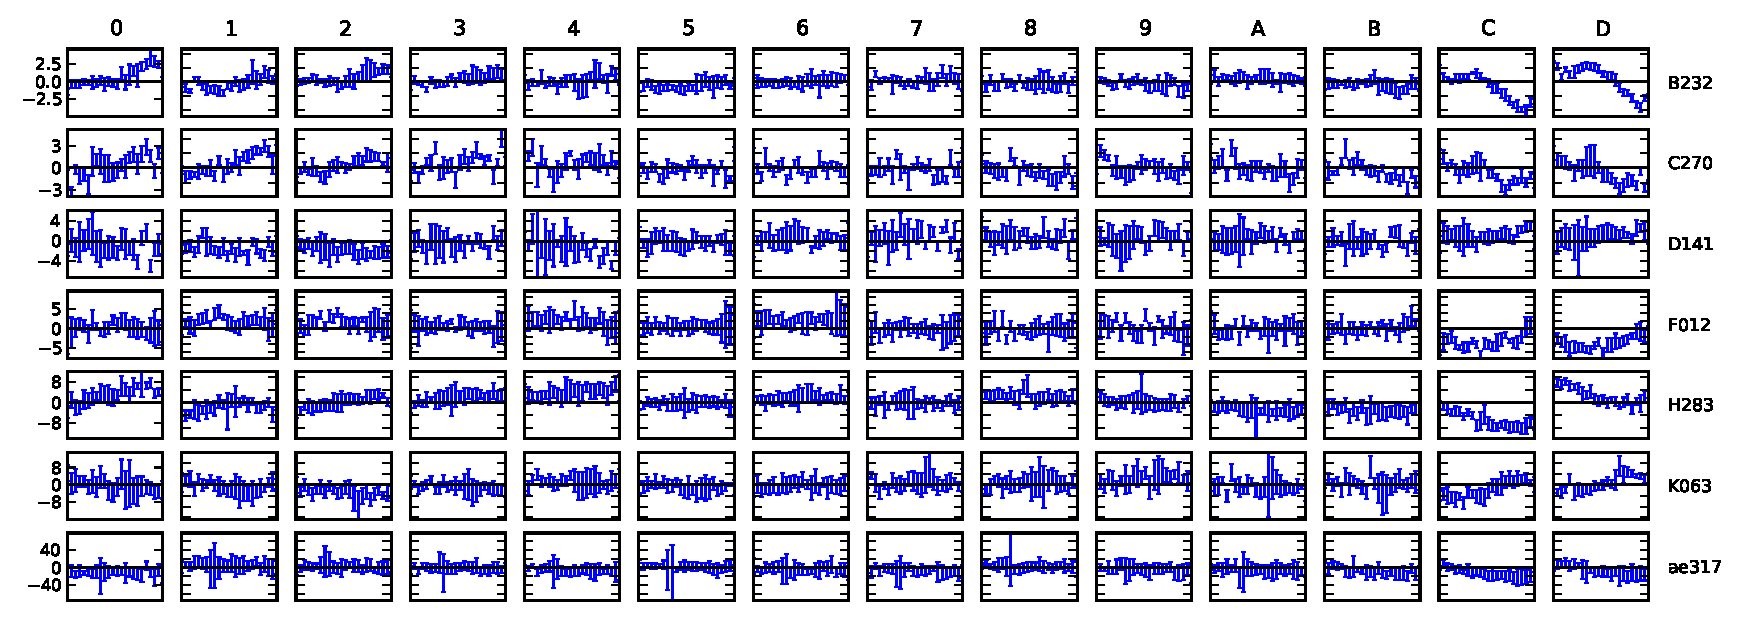
\includegraphics[width=12cm]{o2006_dEphase_mean}
}
\caption{\label{fig:dEphase}Differential gain-phases ($\arg\Delta\jones{E}{}$, in degrees) as a function of time for the 2003 (top) and 2006 (bottom) observations. Rows correspond to sources, columns to antennas. The vertical plot scale is fixed within each row, but differs from row to row. Horizontal lines indicate the $\arg\Delta\jones{E}{}=0$ level.}
\end{figure*}

Figure~\ref{fig:dEampl} is a summary of the differential gain-amplitudes per source, per antenna. The precise quantity plotted here was computed as follows. First, I computed the norm of the $\Delta\jones{E}{}$ matrix (diagonal by construction) as 

\[
\left|\left|\matrixtt{a}{0}{0}{b}\right|\right| \equiv \sqrt{|a|+|b|},
\]

i.e. as the geometric mean of the X and Y gain-amplitudes. I then normalized (divided) this value by the mean value per source (that is, the mean across all time intervals, bands, and antennas), which was meant to take out the effect of incorrect model fluxes (see below). The resulting ``normalized norm'' was then plotted as a function of time, per source, per antenna.

Figure~\ref{fig:dEphase} is a similar plot of the differential gain-phases, computed as

\[
\arg\matrixtt{a}{0}{0}{b} \equiv \frac{\arg a + \arg b}{2}.
\]

The most striking feature of Figs.~\ref{fig:dEampl} and \ref{fig:dEphase} is the high SNR. They show a high degree of temporal continuity in the solutions, and statistically significant structure. This strongly suggests that the solutions represent real physical or numerical effects. As to the nature of these effects, I still do not have satisfactory answers, though it is hoped that the ``QMC Project'' mentioned earlier will shed some more light on the issues. The rest of this section discusses some of the more prominent questions, and proposes some rather speculative explanations.
 
\subsection{Absorbing errors in the sky model\label{sec:de-analysis-model}}

As already mentioned, a major caveat of the flyswatter approach is that $\Delta\jones{E}{}$ solutions will tend to absorb inaccuracies in the source model. By analogy (and for exactly the same reasons), classic selfcal 
alone cannot solve for absolute positions or fluxes. Indeed, if the true position of a source $\vec l = (l,m)$ is offset from the model position $\vec l^\mathrm{(mod)} = \vec l + \delta\vec l = (l+\delta l,m + \delta m)$, while the true brightness $\coh{B}{}$ differs from the model brightness by a multiplicative matrix factor: $\coh{B}{}^\mathrm{(mod)} = \jones{A}{} \coh{B}{} \jonesT{A}{}$ (the latter being a straightforward generalization of a scalar factor $a^2$), then the coherency term of the RIME for the model source may be written out as

\begin{eqnarray*}
\coh{X}{pq}^\mathrm{(mod)} & = & K_{p}(\vec l + \delta\vec l) \coh{B}{}^\mathrm{(mod)} K^\herm_{q}(\vec l + \delta\vec l) \\
 & = & K_{p}(\delta\vec l) K_{p}(\vec l) \jones{A}{}\coh{B}{}\jonesT{A}{} K^\herm_{q}(\vec l) K^\herm_{q}(\delta\vec l) \\
 & = & [ K_{p}(\delta\vec l)\jones{A}{}]\cdot[K_{p}(\vec l)\coh{B}{}K^\herm_{q}(\vec l)]\cdot[K_{q}(\delta \vec l)\jones{A}{}]^\herm \\
 & = & [K_{p}(\delta\vec l)\jones{A}{}] 
       \cdot \coh{X}{pq} \cdot 
       [K_{q}(\delta\vec l)\jones{A}{}]^\herm.
\end{eqnarray*}

If a solvable differential gain is then assigned to the source, the model can be made to fit the data by absorbing the $K_{p}(\delta\vec l)\jones{A}{}$ factor into the $\Delta\jones{E}{ps}$ solutions.

Even more insidiously, differential gains can absorb some source structure. Consider a source that is slightly extended in one direction, enough to be resolved on the longest baselines. An E-W array like the WSRT has a one-dimensional instantaneous {\em fan beam}. It will ``see'' the source as a point source when the fan beam is aligned with the source orientation, and start resolving it when the fan beam becomes perpendicular to the source. In other words, the apparent flux of the source will remain constant in time on short baselines, and vary in time on the long baselines as the source resolves. If such a source is represented by a point source in the sky model, the model flux will be constant on all baselines. Now, if some antennas are predominantly involved in long baselines (RTC and RTD, in the case of WSRT), $\Delta\jones{E}{}$ solutions can compensate for some of the flux discrepancy by changing the gain-amplitudes of these antennas. I would expect to see a variation of $||\Delta\jones{E}{}||$ with a 12-hour period. Since most of the baselines to RTC and RTD are mutually redundant (0-C equals 1-D, etc.), their variation in $||\Delta\jones{E}{}||$ should be very similar. 

This is exactly what we're seeing in Fig.~\ref{fig:dEampl}! The plots very strongly suggest that the top three sources (B, C and D) are indeed slightly extended (more so than in the model, that is). If this is the case, then the dominant contribution to $||\Delta\jones{E}{}||$ on antennas RTC and RTD is due to source structure rather than any actual DDE. 

\subsection{Amplitude behaviour}

If the behaviour of differential amplitude on RTC and RTD is due to source structure, this still leaves effects on the other antennas unexplained. First let us consider what a pointing error would look like. With the exception of source ae317 (for which the solutions are much too noisy anyway), the other six sources are well within the main lobe of the primary beam, where the beam gain can be expected to decrease smoothly with distance from pointing center. We should therefore expect to see $||\Delta\jones{E}{sp}||>1$ if antenna $p$ mispoints \emph{towards} source $s$ (the source appears brighter on antenna $p$), and $||\Delta\jones{E}{sp}||<1$ if it mispoints \emph{away}. WSRT dishes are equatorially mounted, so mispointings due to mechanical or electronic errors in either axis drive would be stationary with respect to the sky, and thus cause constant 
$||\Delta\jones{E}{}||$ offsets. Mispointings due to wind pressure, thermal or gravitational deformation, on the other hand, would be intrinsically time-variable (but would perhaps correlate between adjacent antennas).

Quite a few plots in Fig.~\ref{fig:dEampl} do show (mostly) static offsets. It can be illuminating to present $||\Delta\jones{E}{}||$ in a format I call the ``rogues gallery'' (Figs.~\ref{fig:rogues-2003} and \ref{fig:rogues-2006}). This shows, for each of the 14 antennas, a 12-hour average $||\Delta\jones{E}{}||$ per source, using circles of varying size placed at the position of the source. The magnitude of $(||\Delta\jones{E}{}||-1)$ is indicated by circle size, and the sign by colour. A static mispointing in, e.g., a Northern direction would show up as blue circles in the top half of the plot (i.e. sources appearing brighter), and red circles in the bottom half.

\newlength{\roguewidth}
%\setlength{\roguewidth}{2.4cm} % for 12 cm figure
%\setlength{\roguewidth}{3.4cm} % for double-column figure
\setlength{\roguewidth}{.2\columnwidth} % for single-column figure

%plot-de-solutions.py --circle-ampl -o eps --portrait --radius 40 --circle-borders 0.05,0.98,0.05,0.9 --circle-title-fontsize 40 -r o2003.cache --circle-minsize=0 --circle-maxsize=200 --circle-label-fontsize=0 --circle-axis-fontsize=10 --output-prefix o2003
%plot-de-solutions.py --circle-ampl -o eps --portrait --radius 40 --circle-borders 0.05,0.98,0.05,0.9 --circle-title-fontsize 40 -r o2006.cache --circle-minsize=0 --circle-maxsize=200 --circle-label-fontsize=0 --circle-axis-fontsize=10 --output-prefix o2006

\begin{figure}
\centering
\begin{tabular}{@{}c@{}c@{}c@{}c@{}c@{}}
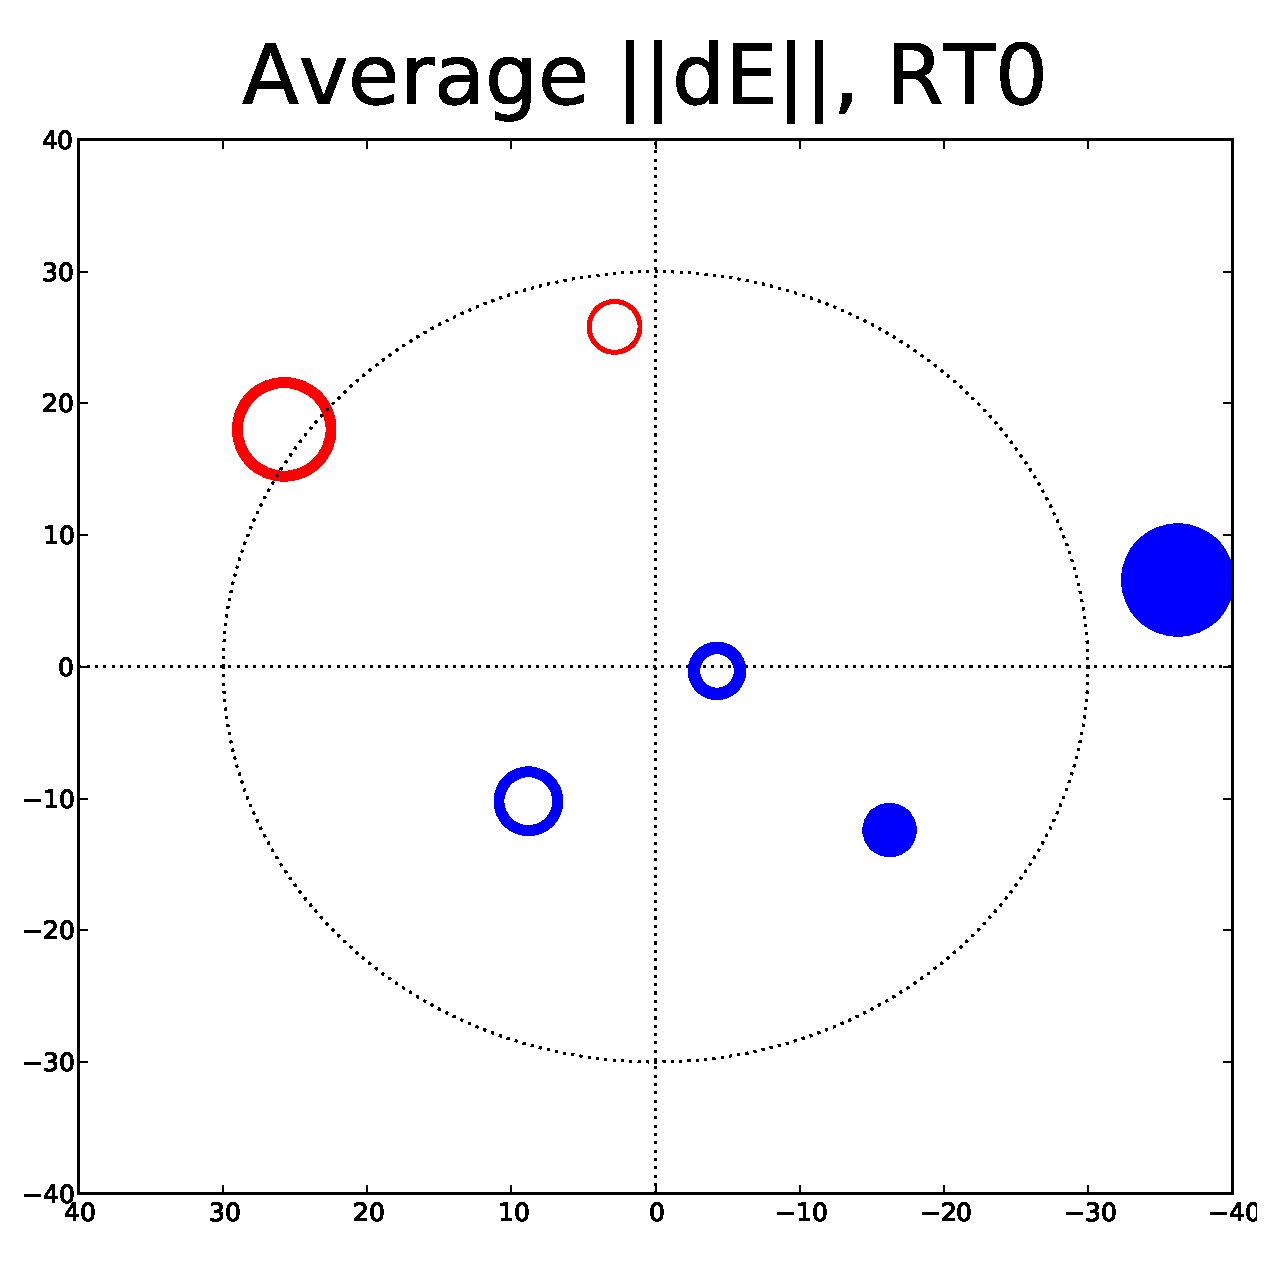
\includegraphics[width=\roguewidth]{o2003_dE_ant0} &
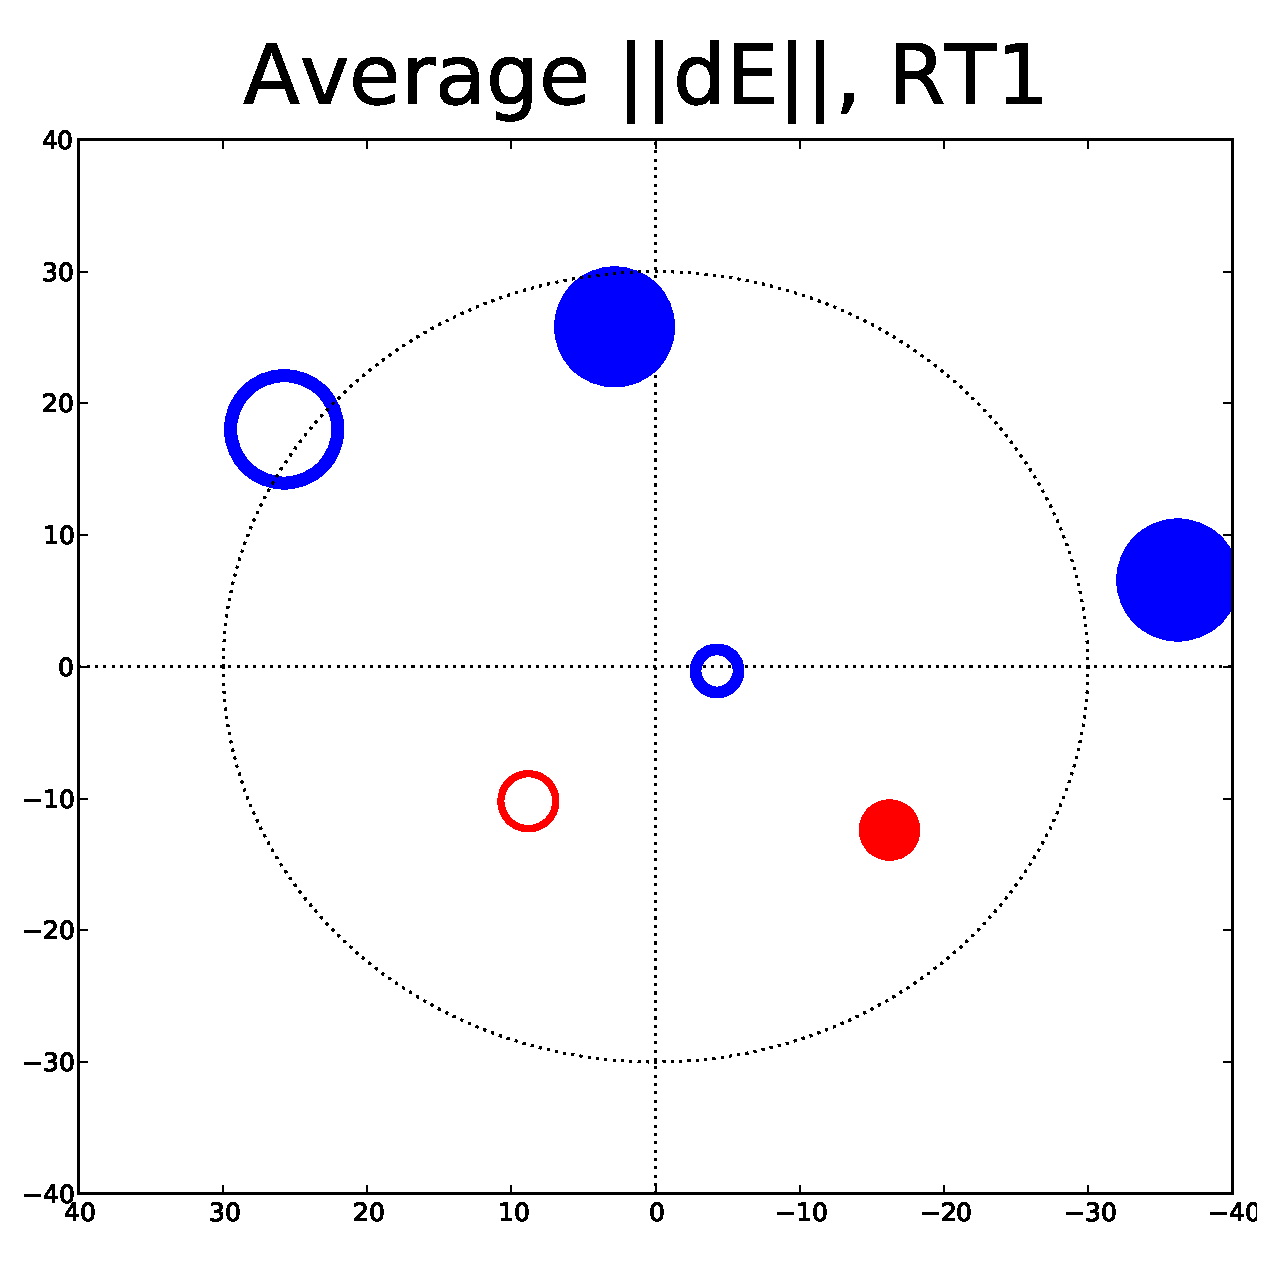
\includegraphics[width=\roguewidth]{o2003_dE_ant1} &
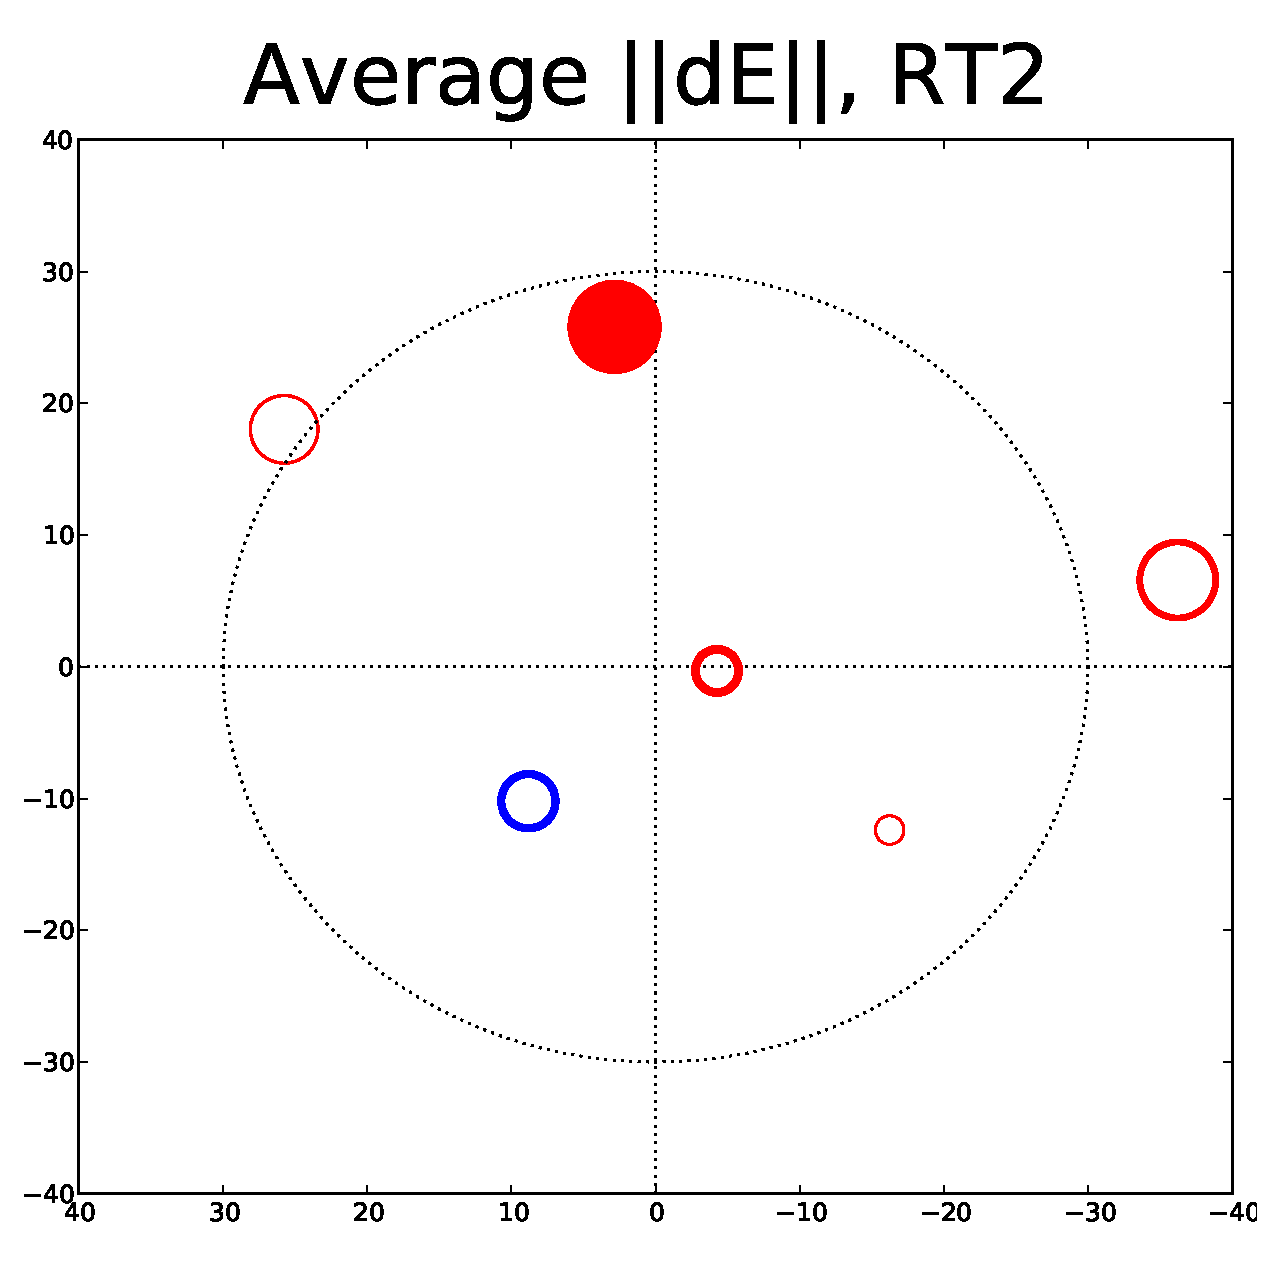
\includegraphics[width=\roguewidth]{o2003_dE_ant2} &
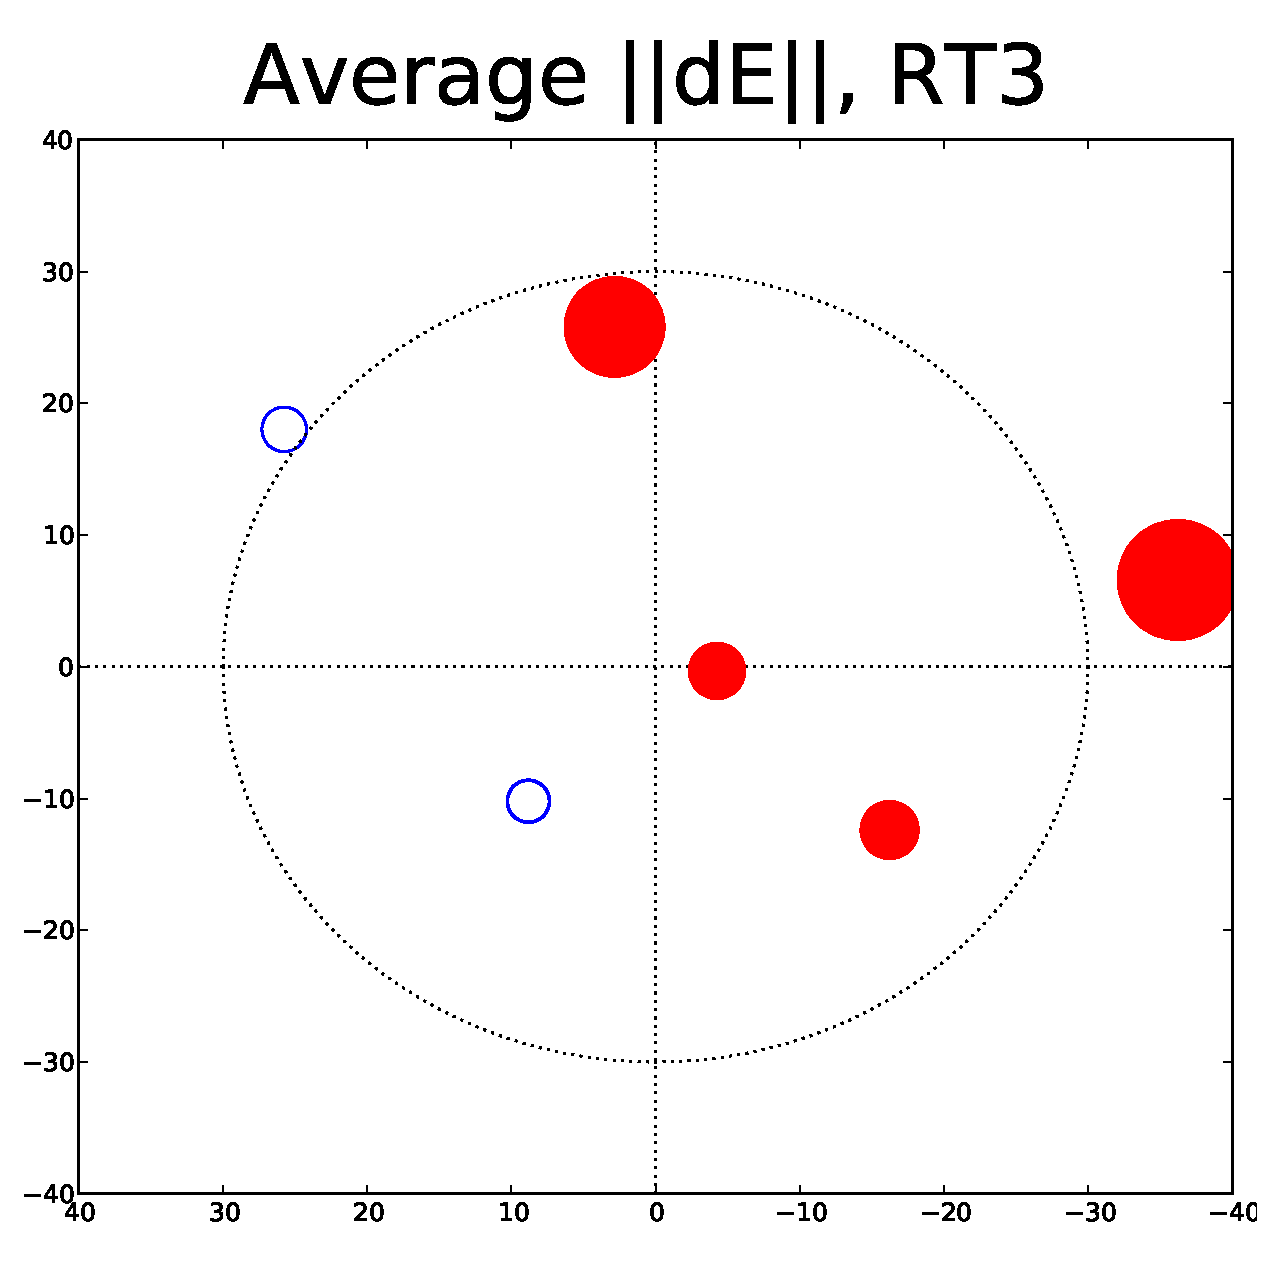
\includegraphics[width=\roguewidth]{o2003_dE_ant3} &
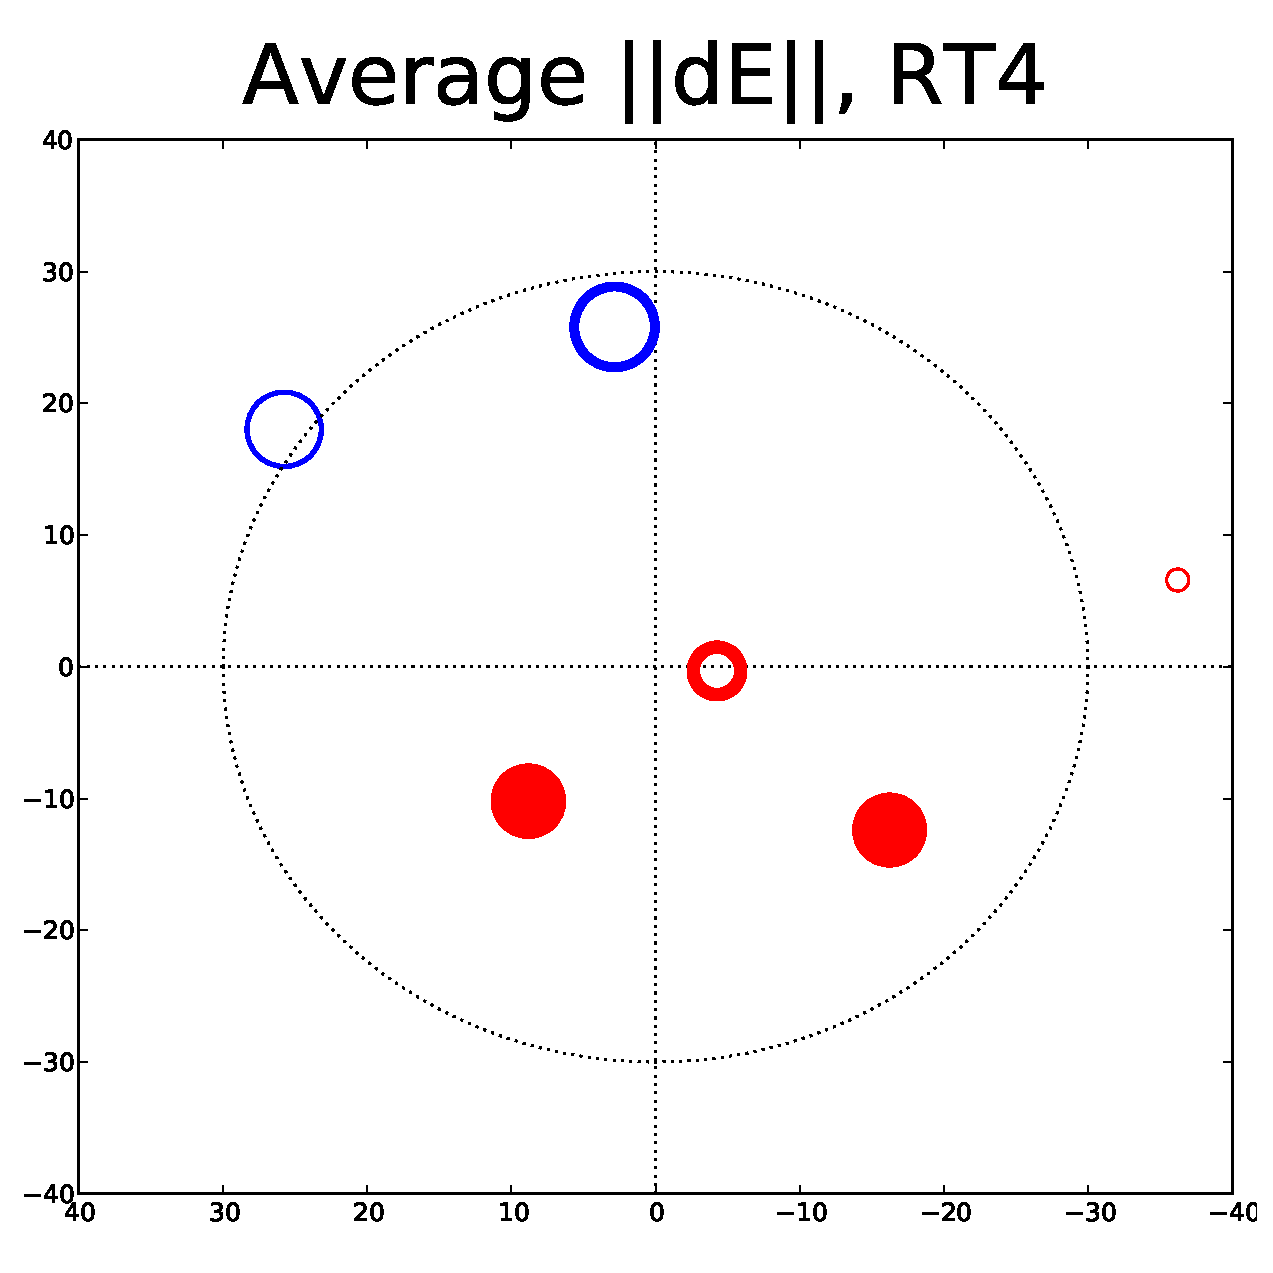
\includegraphics[width=\roguewidth]{o2003_dE_ant4} \\
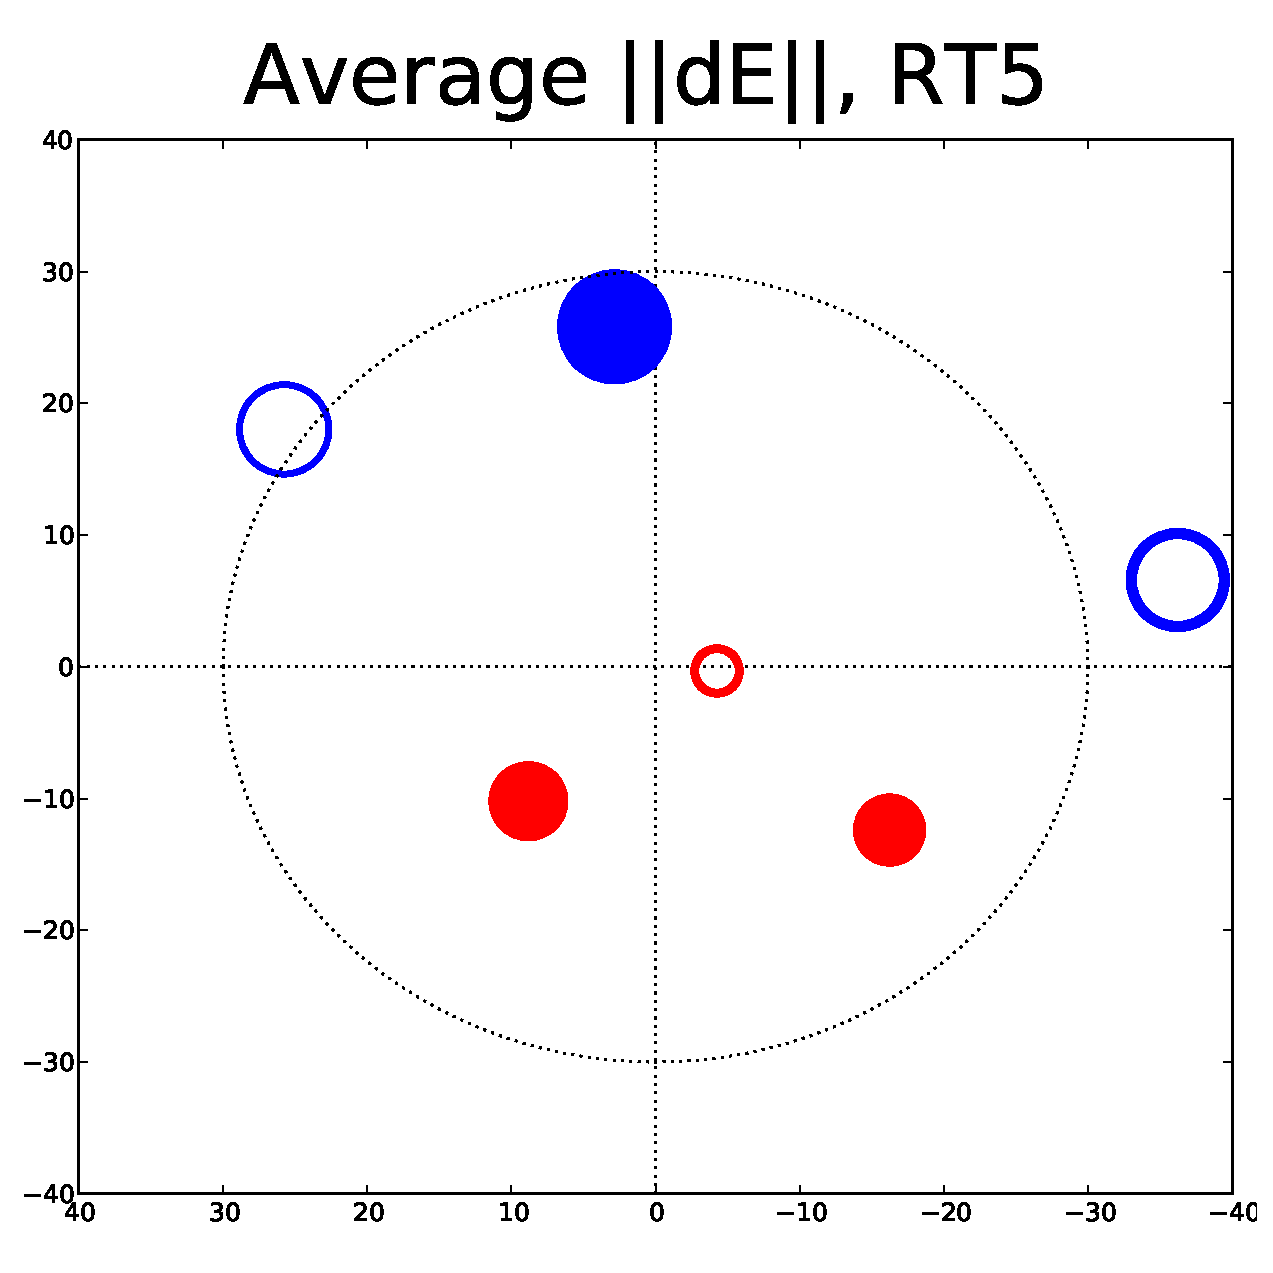
\includegraphics[width=\roguewidth]{o2003_dE_ant5} &
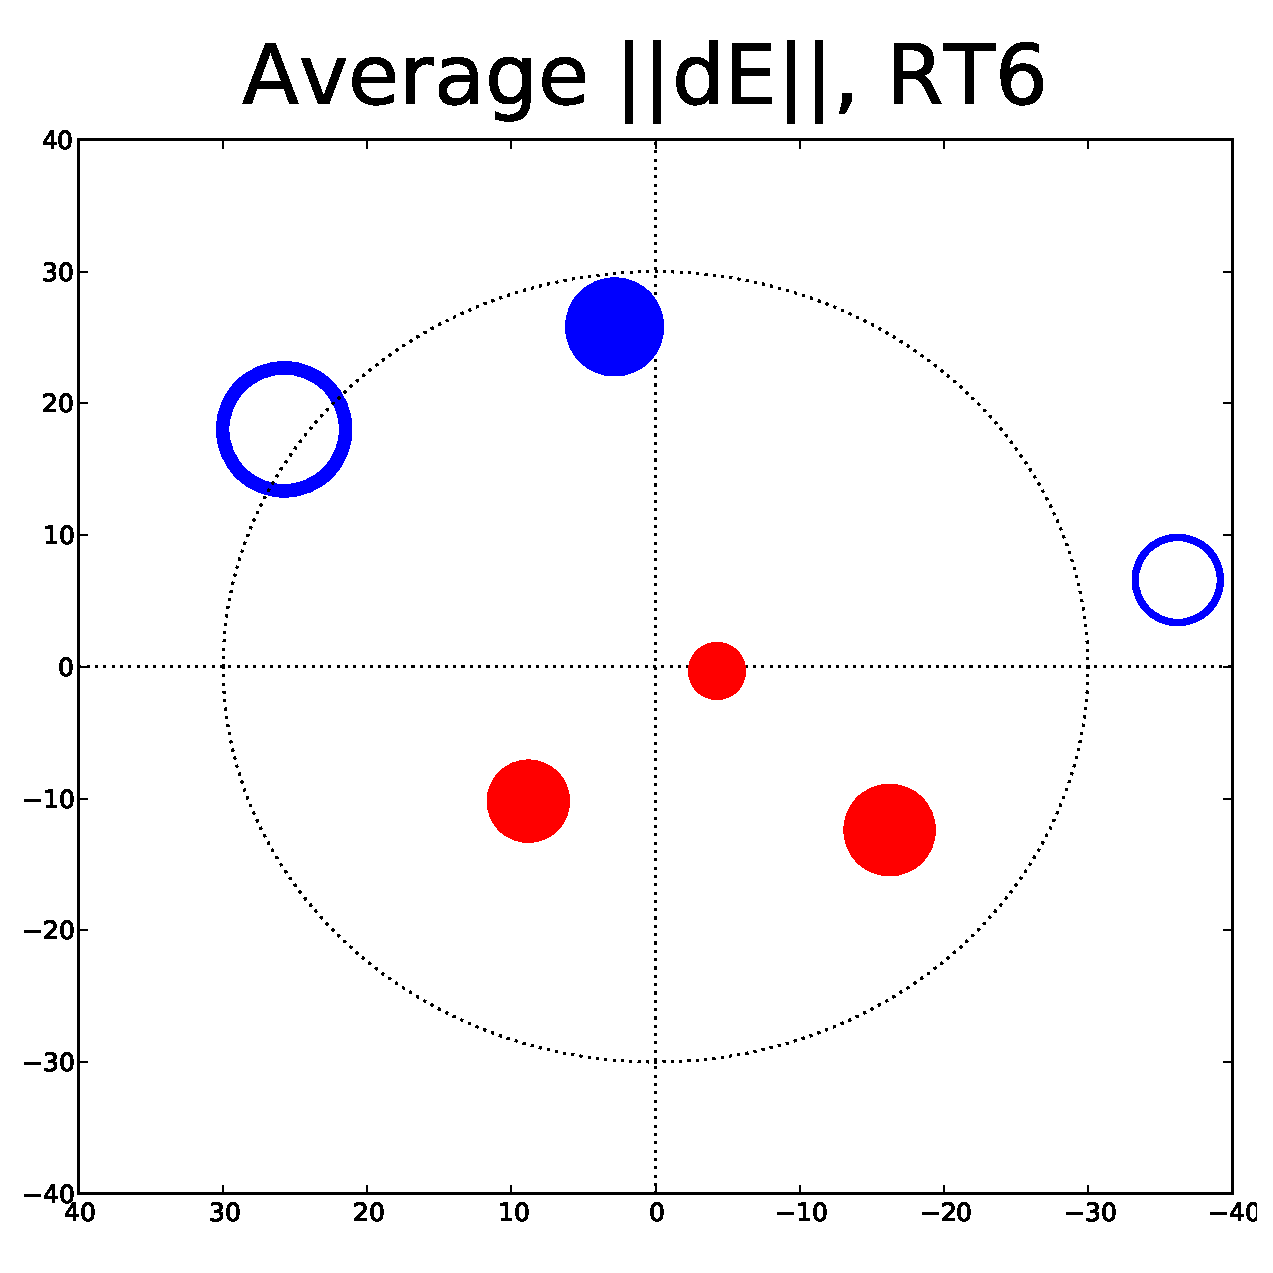
\includegraphics[width=\roguewidth]{o2003_dE_ant6} &
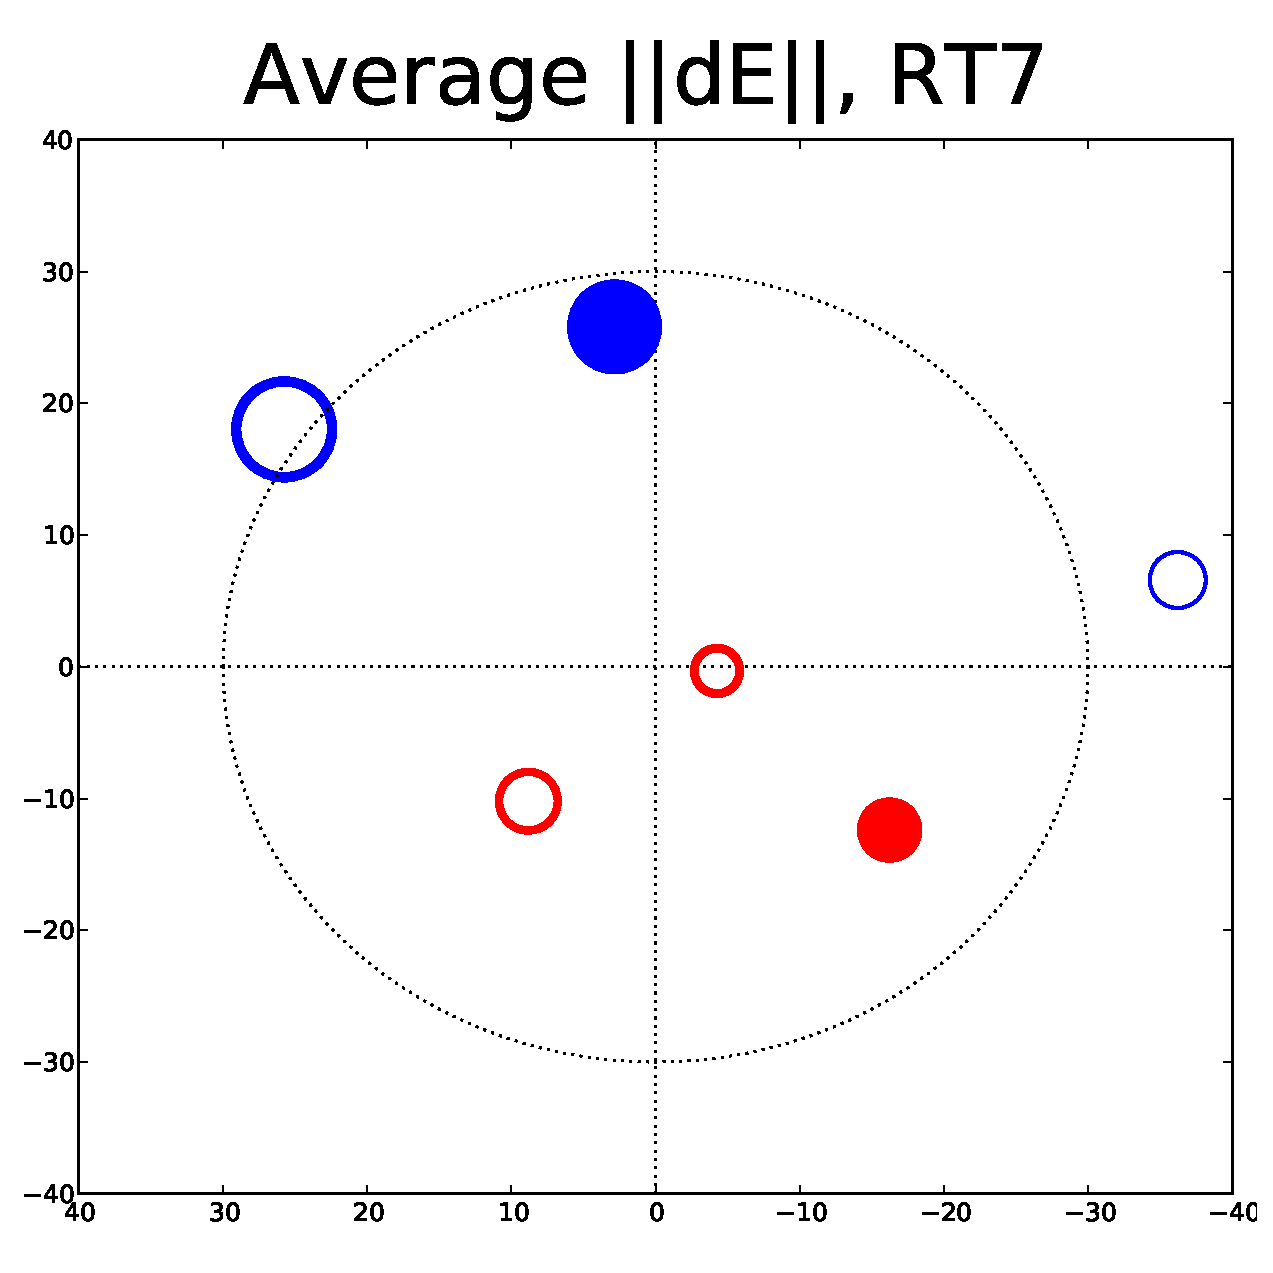
\includegraphics[width=\roguewidth]{o2003_dE_ant7} &
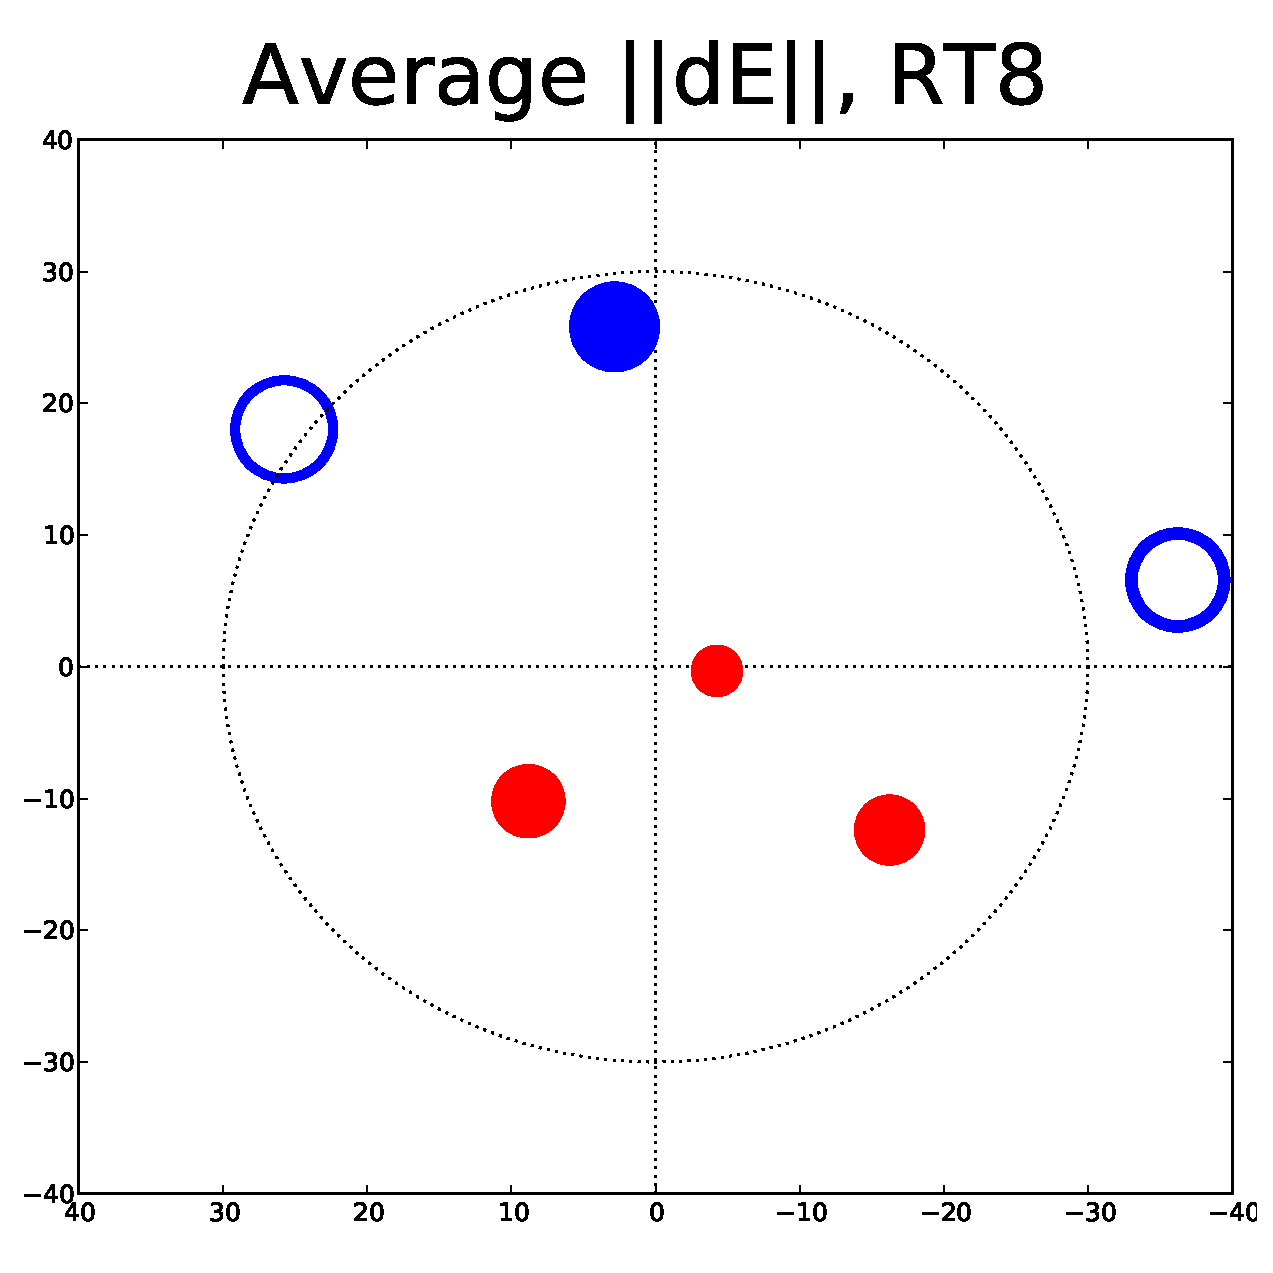
\includegraphics[width=\roguewidth]{o2003_dE_ant8} &
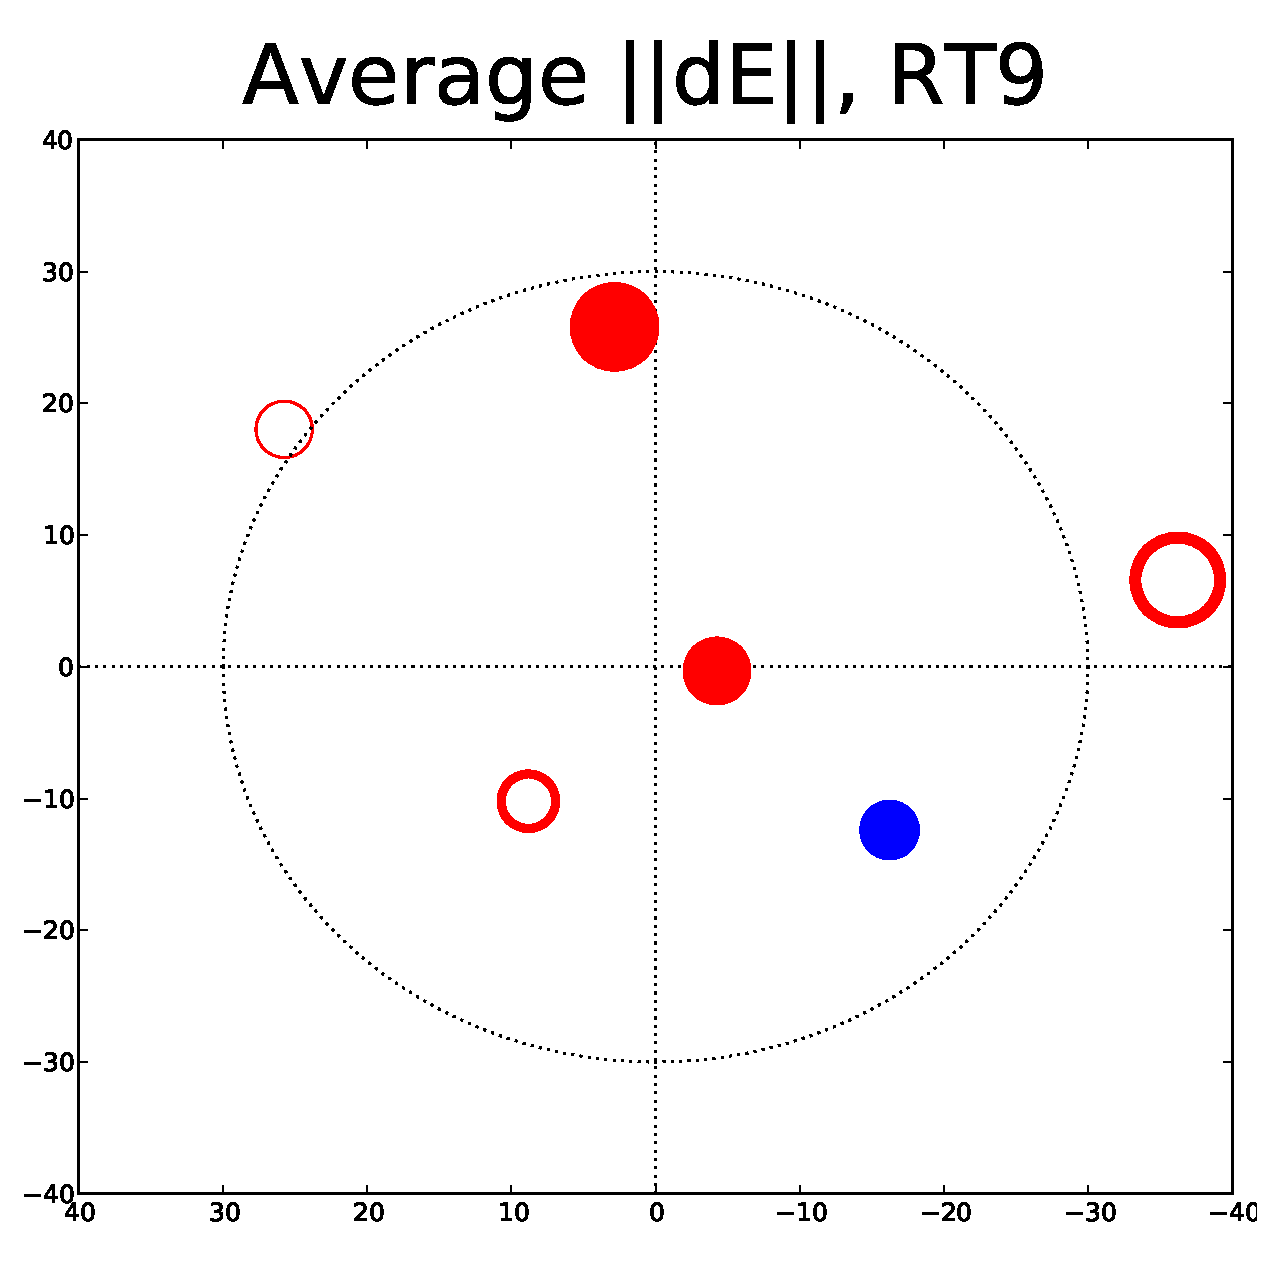
\includegraphics[width=\roguewidth]{o2003_dE_ant9} \\
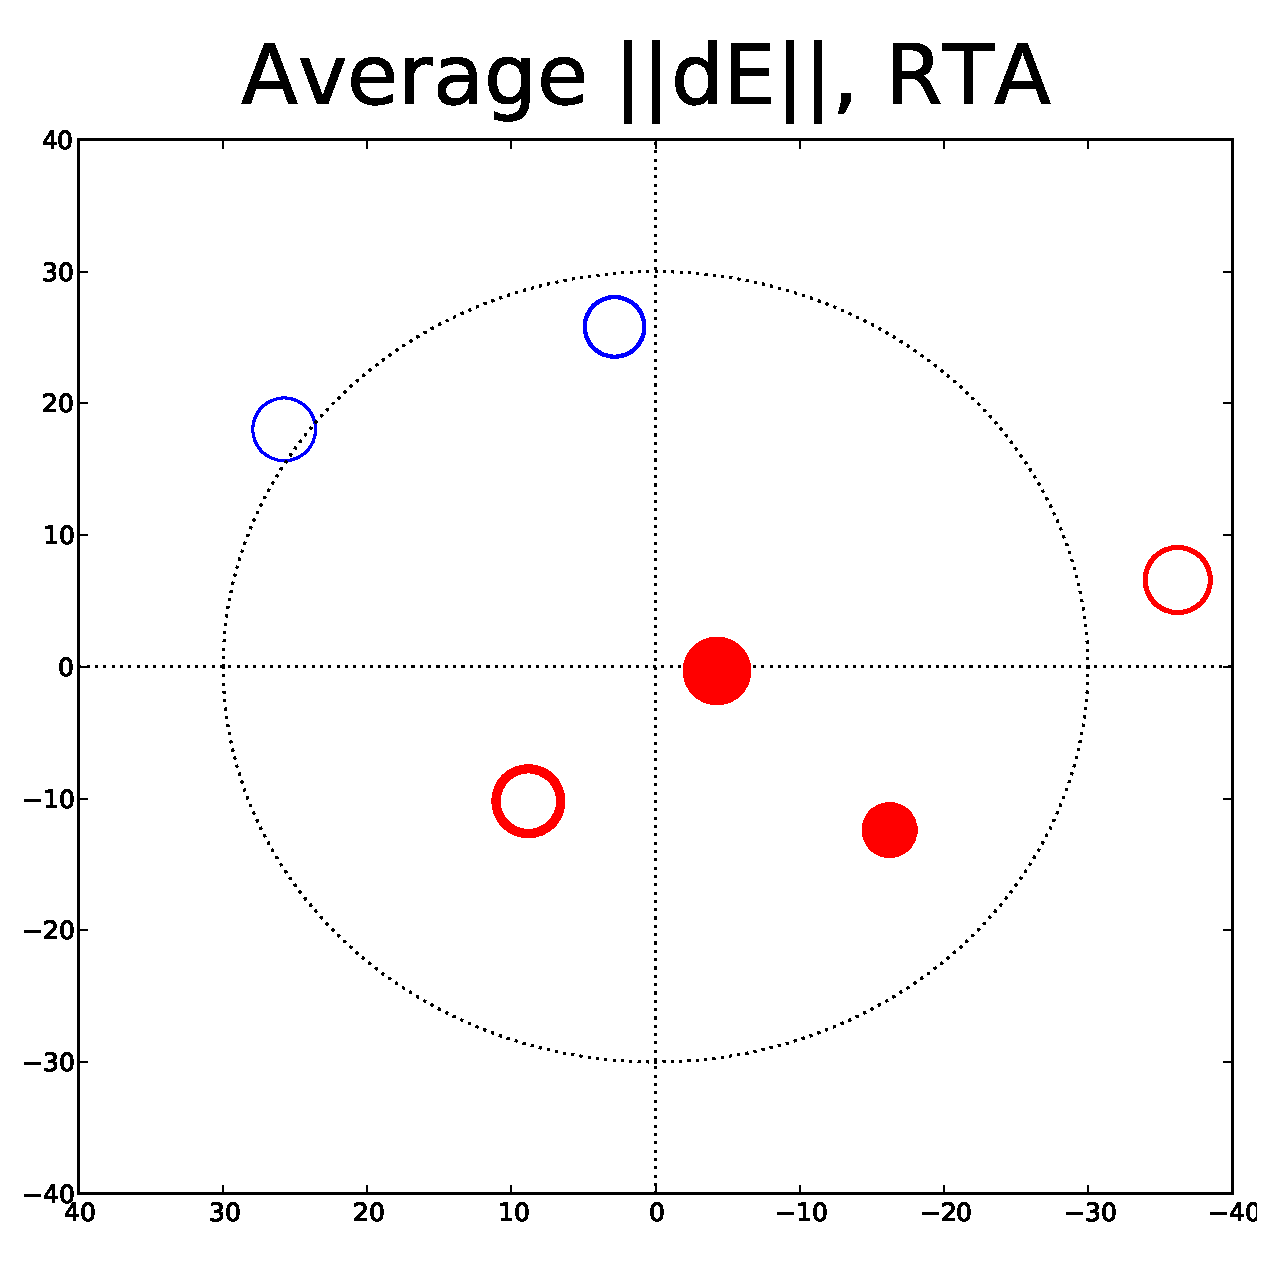
\includegraphics[width=\roguewidth]{o2003_dE_antA} &
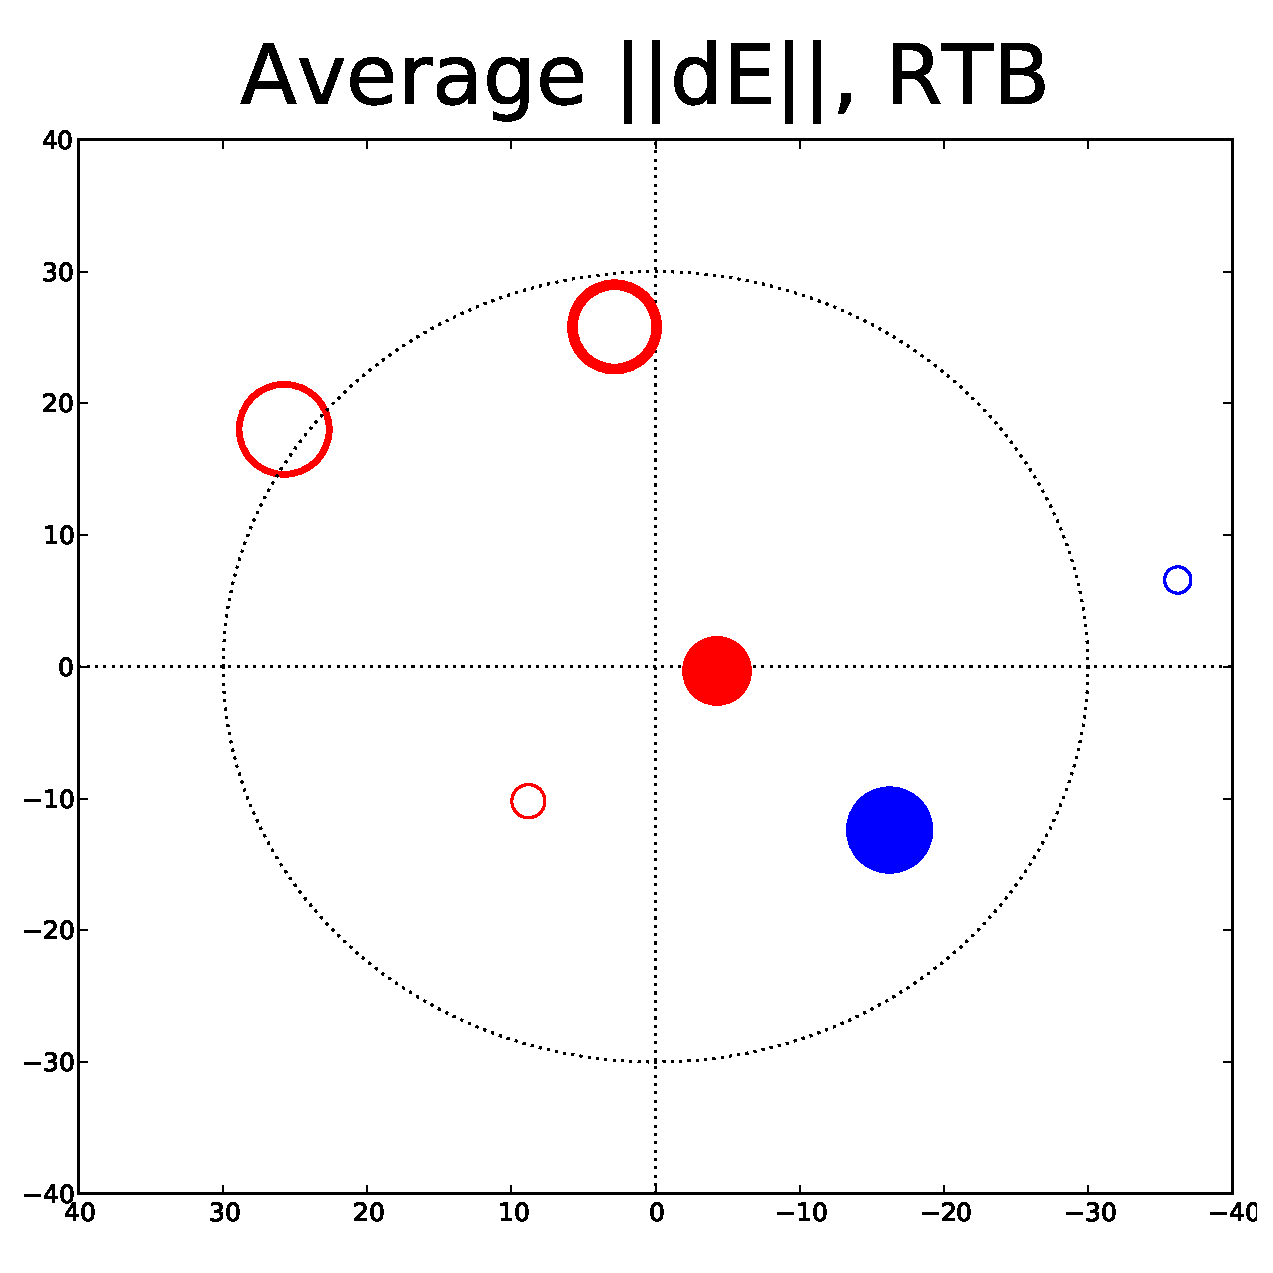
\includegraphics[width=\roguewidth]{o2003_dE_antB} &
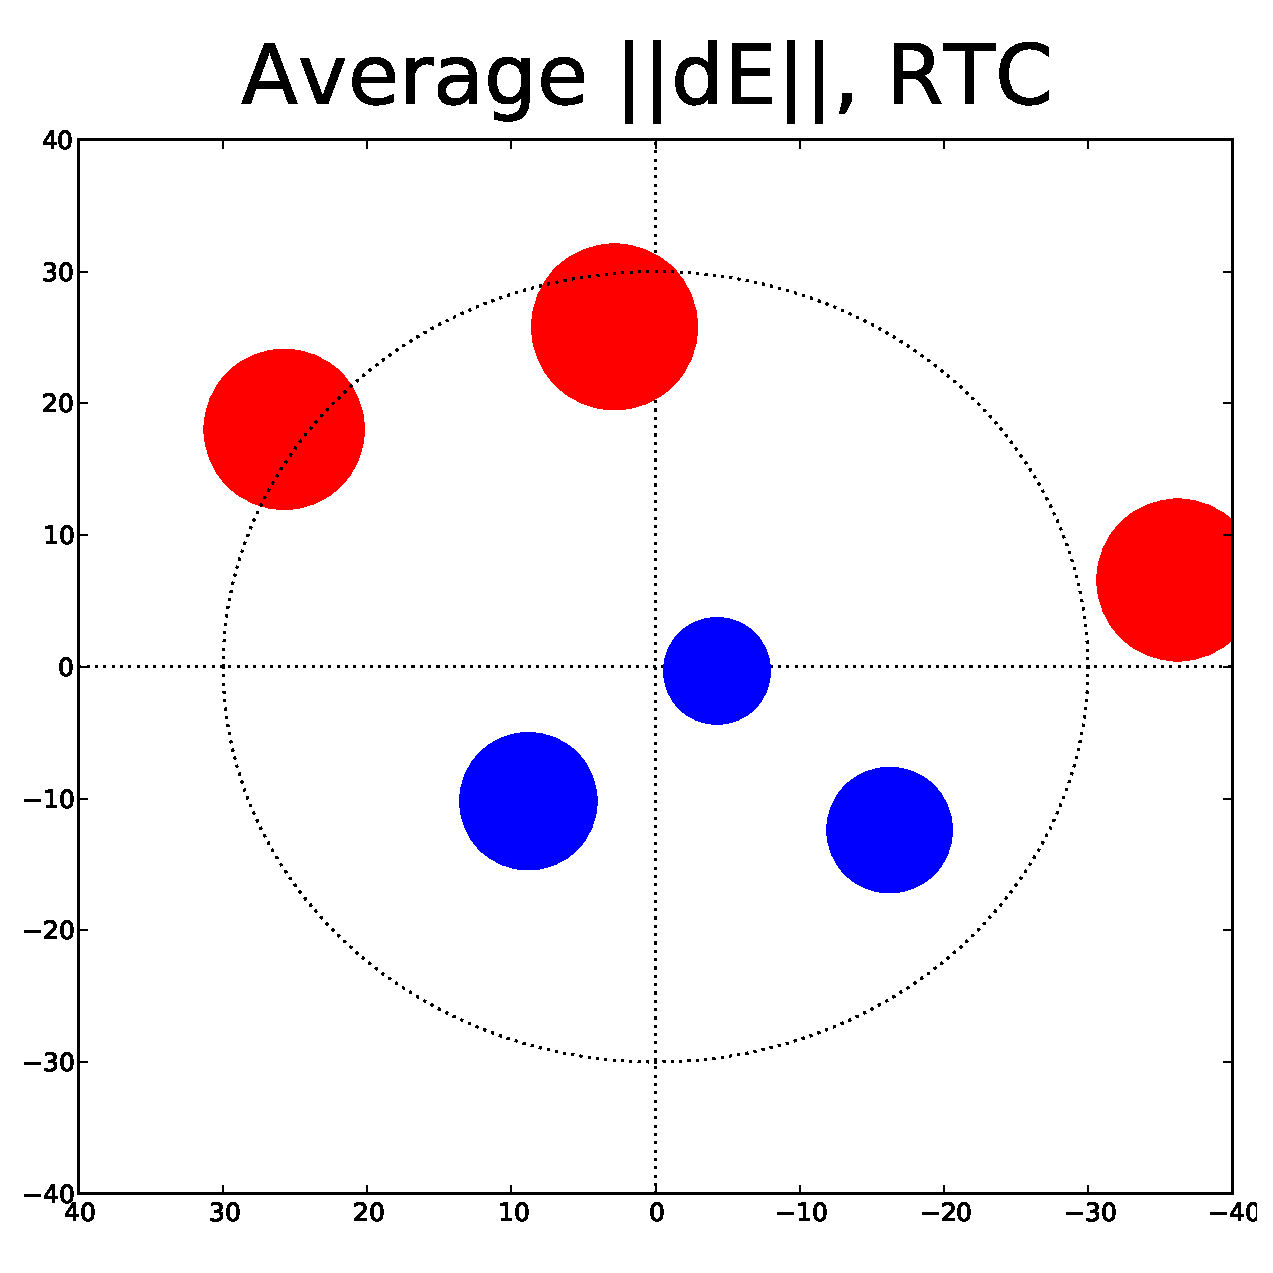
\includegraphics[width=\roguewidth]{o2003_dE_antC} &
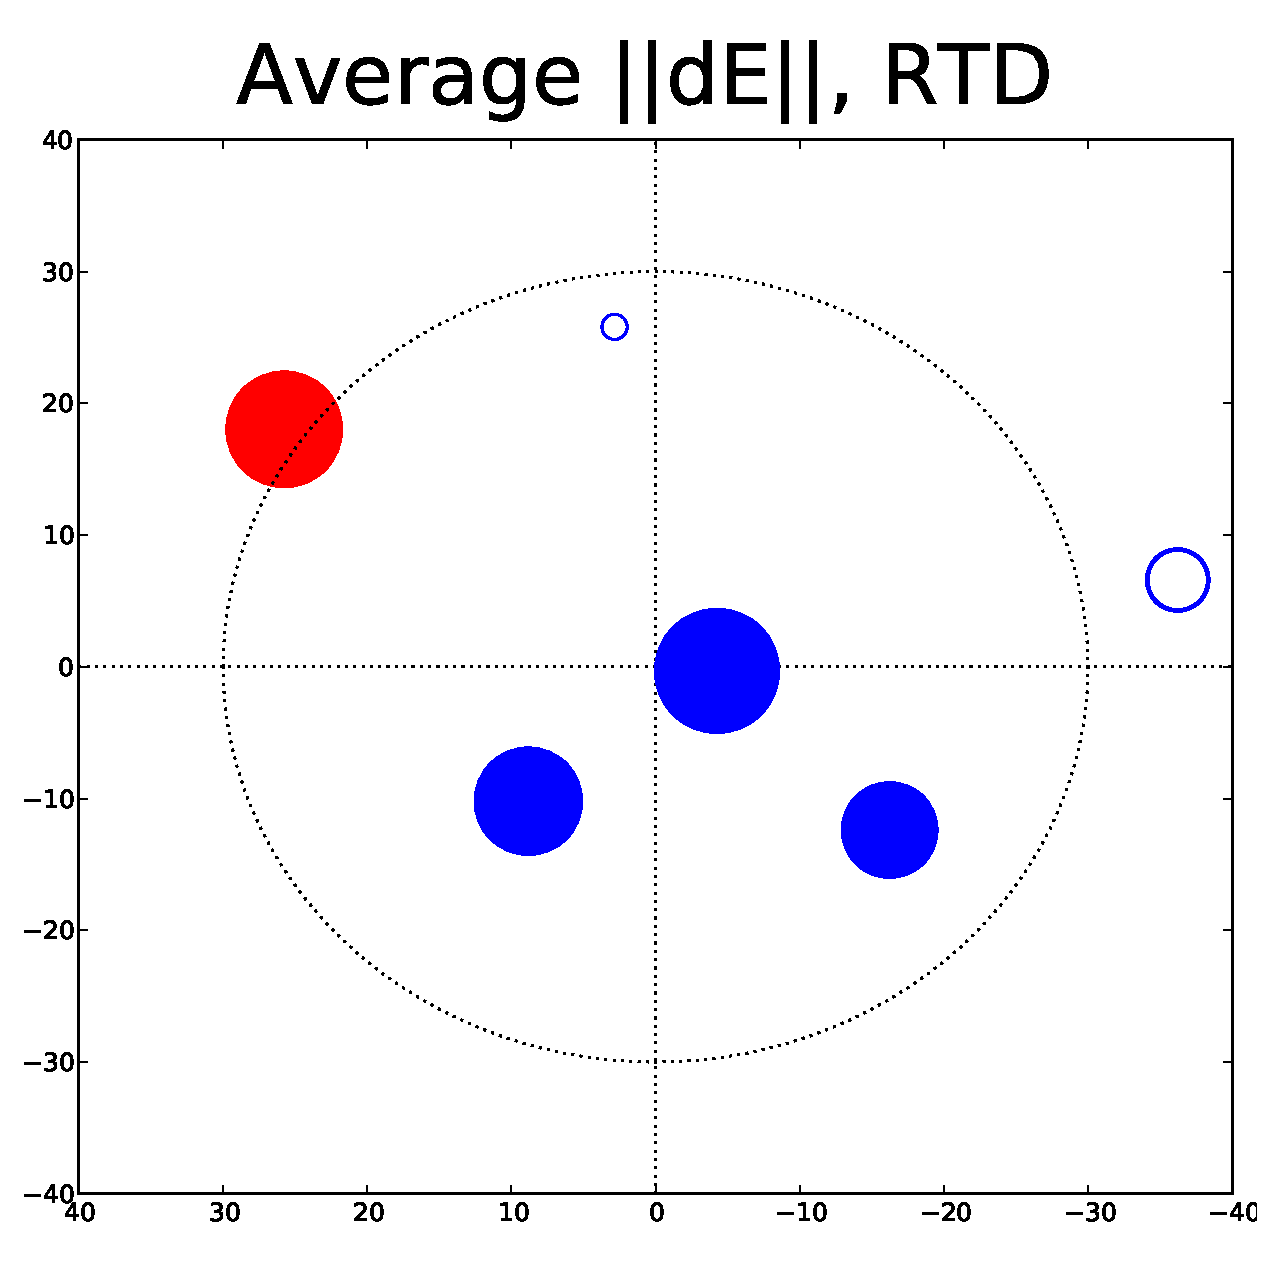
\includegraphics[width=\roguewidth]{o2003_dE_antD} 
\end{tabular}
\caption{\label{fig:rogues-2003}``Rogues gallery'' plot for the 2003 observation. This shows the 12-hour average $||\Delta\jones{E}{}||$ per source, as seen by each antenna. Blue circles correspond to values of $||\Delta\jones{E}{}||>1$, red circles to values of $||\Delta\jones{E}{}||<1$, and areas are proportional to $|\,||\Delta\jones{E}{}||-1\,|$. Line thickness indicates the statistical significance of $|\,||\Delta\jones{E}{}||-1\,|$; filled circles are for detections of over $3\sigma$. The large grid circle is at radius $30\arcmin$.}
\end{figure}

\begin{figure}
\centering
%\sidecaption
\begin{tabular}{@{}c@{}c@{}c@{}c@{}c@{}}
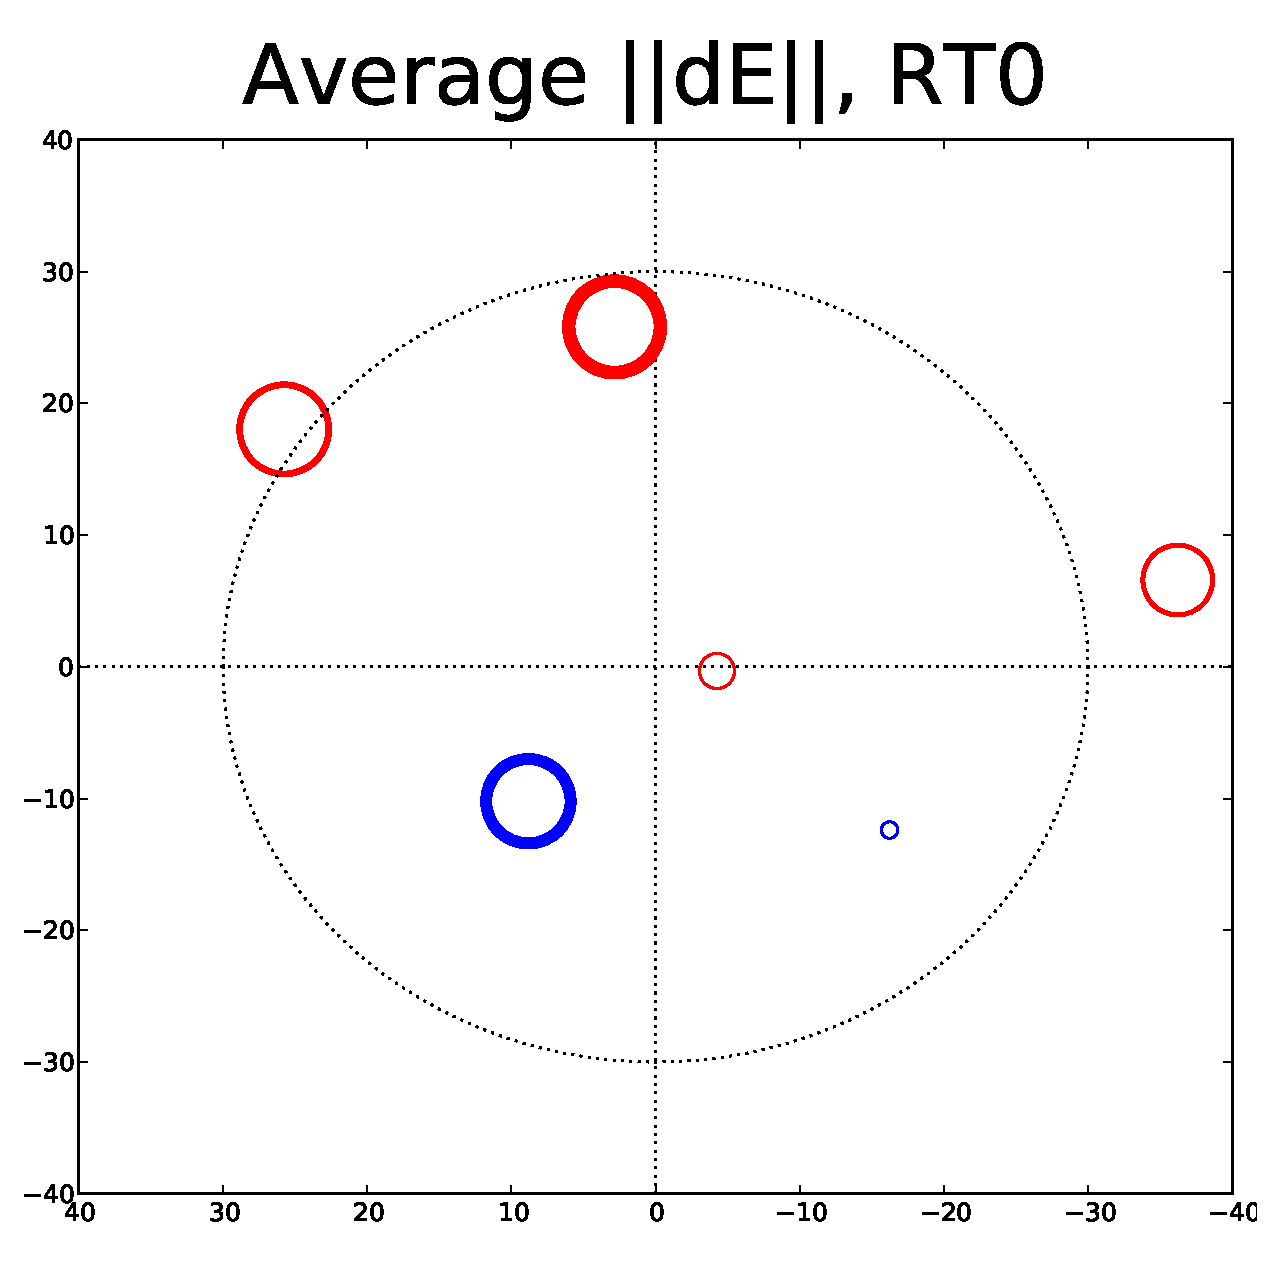
\includegraphics[width=\roguewidth]{o2006_dE_ant0} &
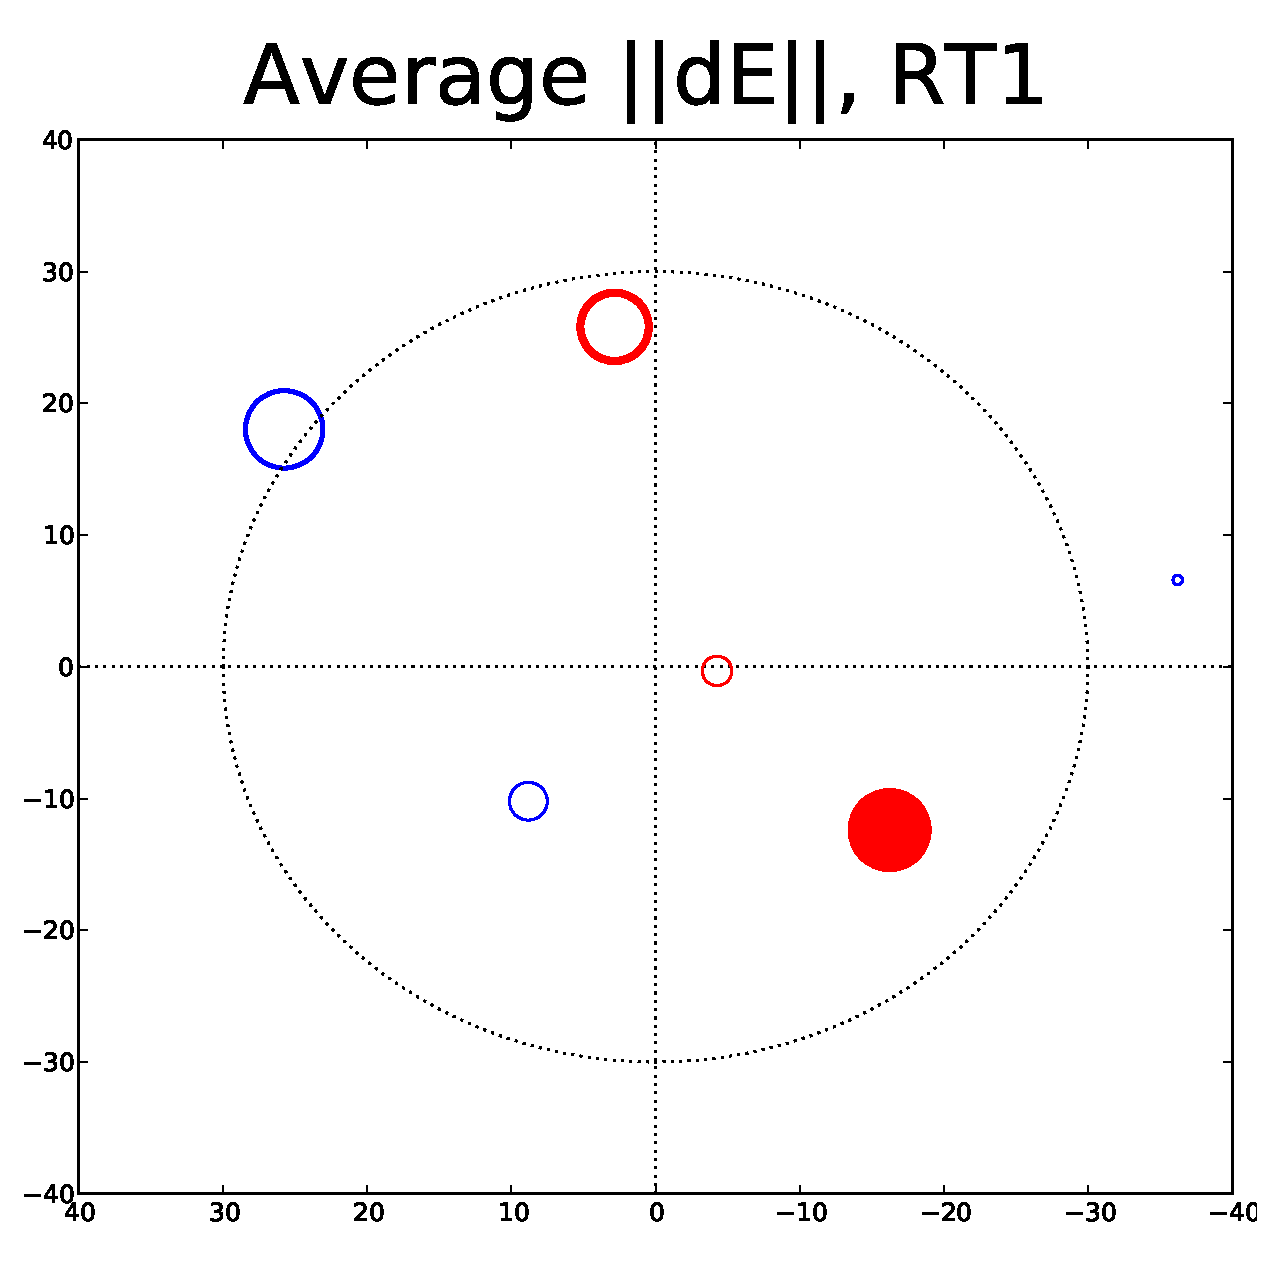
\includegraphics[width=\roguewidth]{o2006_dE_ant1} &
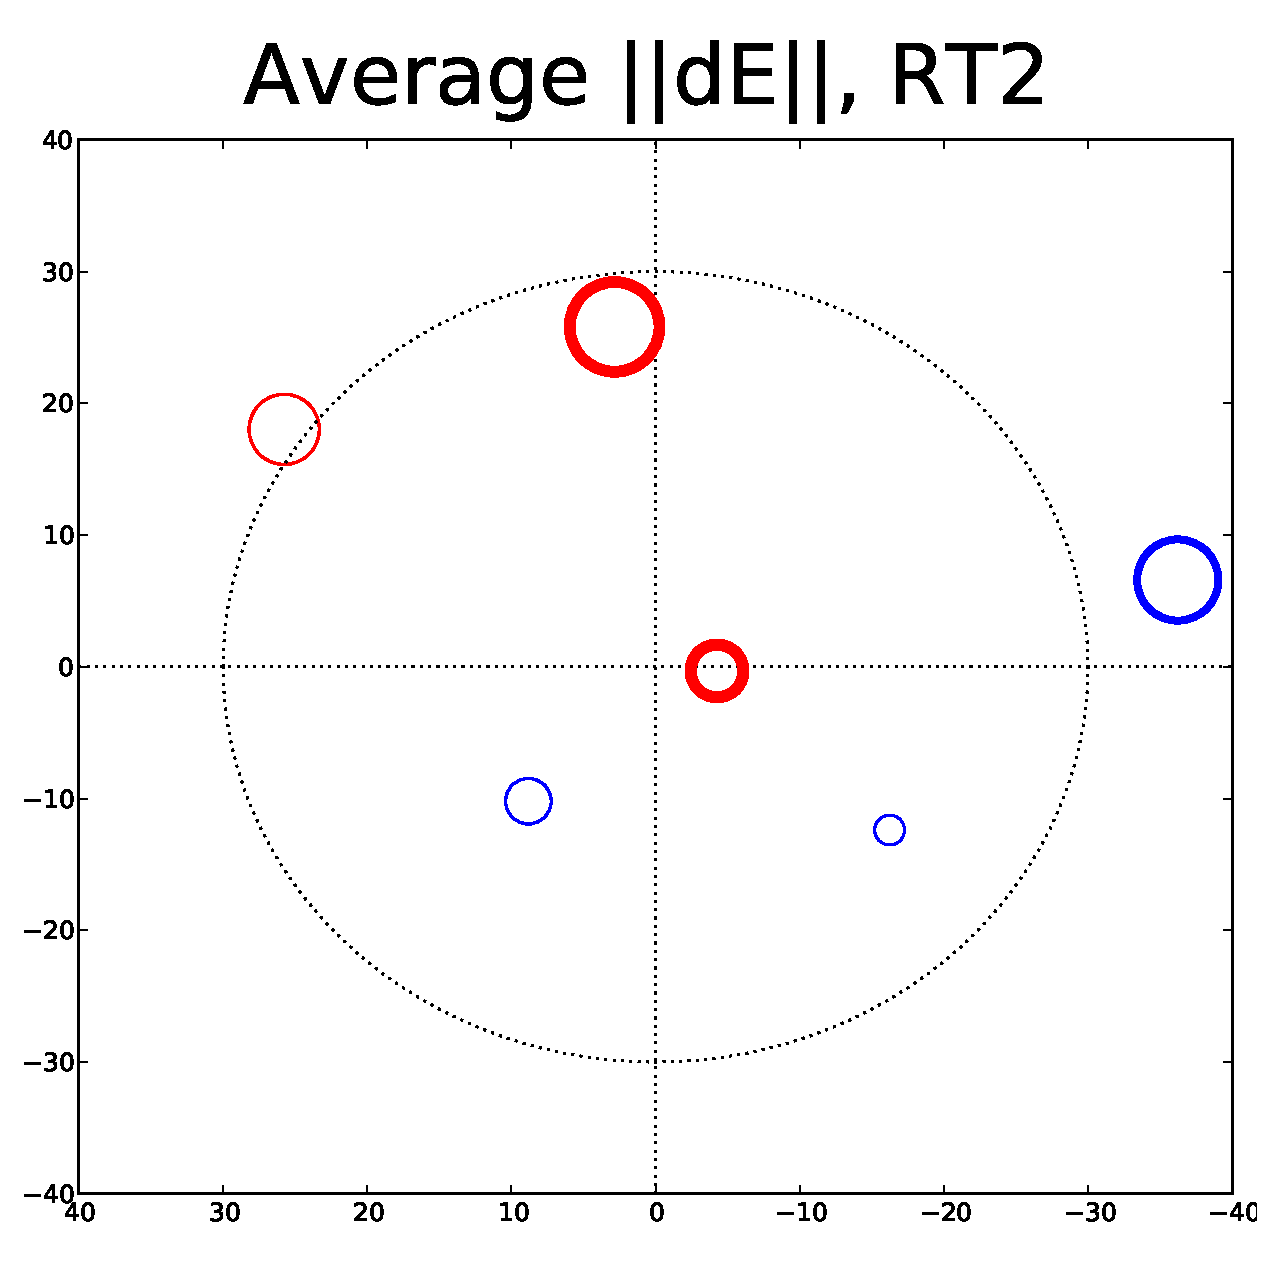
\includegraphics[width=\roguewidth]{o2006_dE_ant2} &
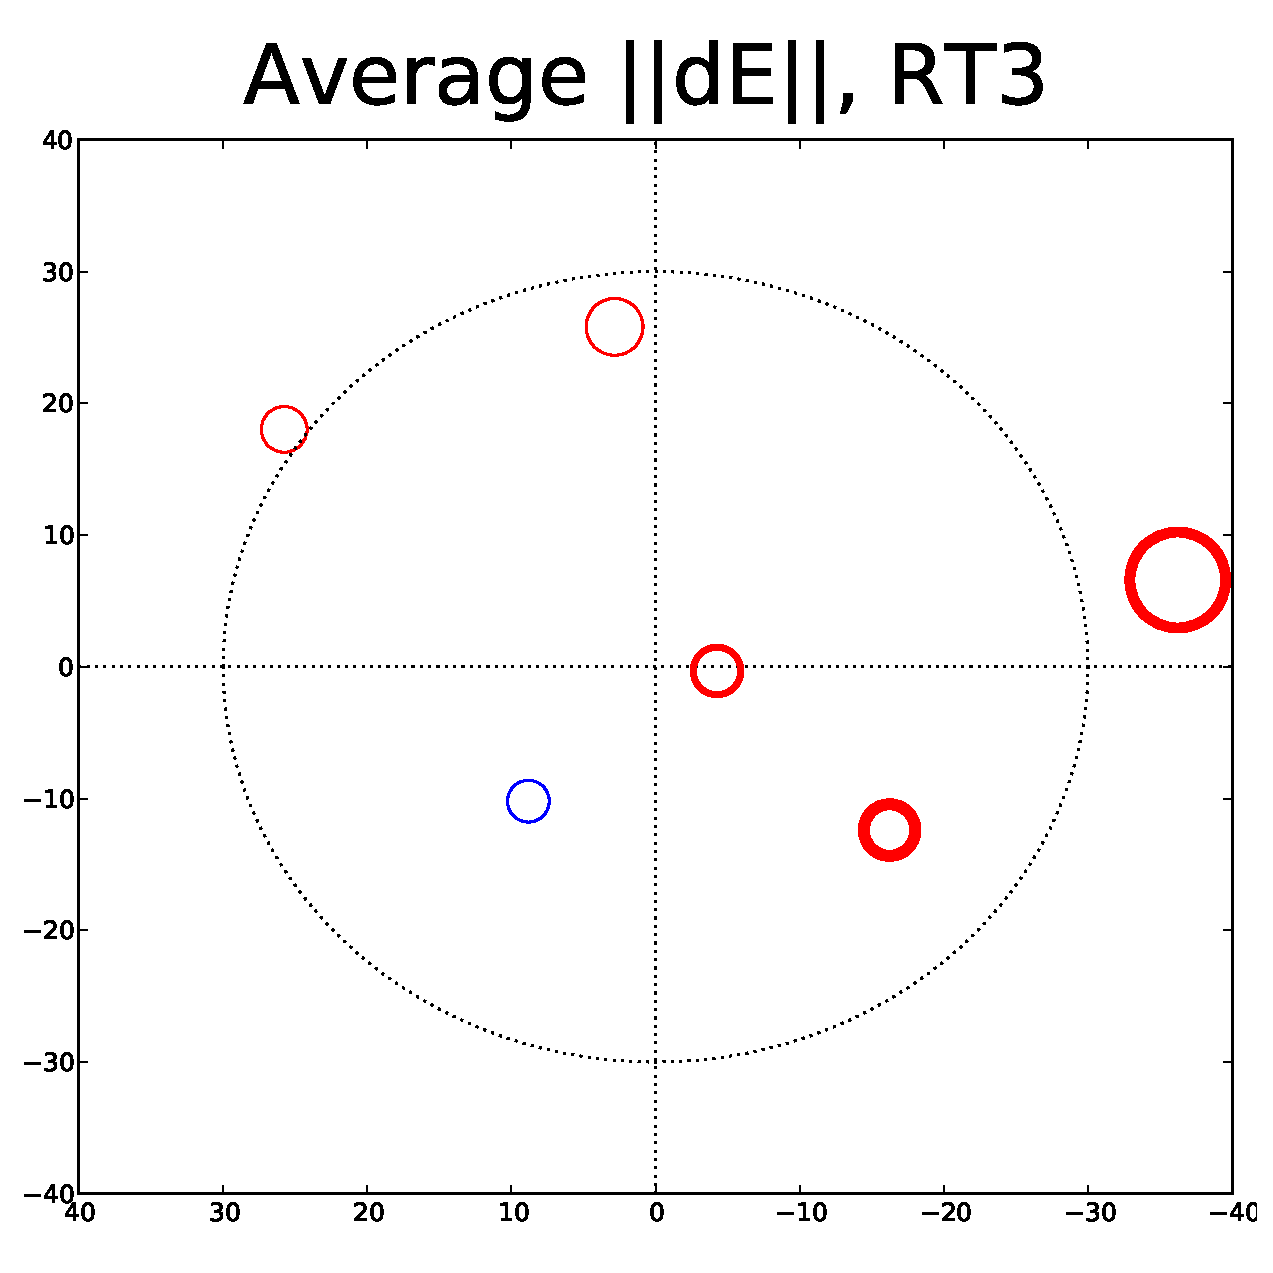
\includegraphics[width=\roguewidth]{o2006_dE_ant3} &
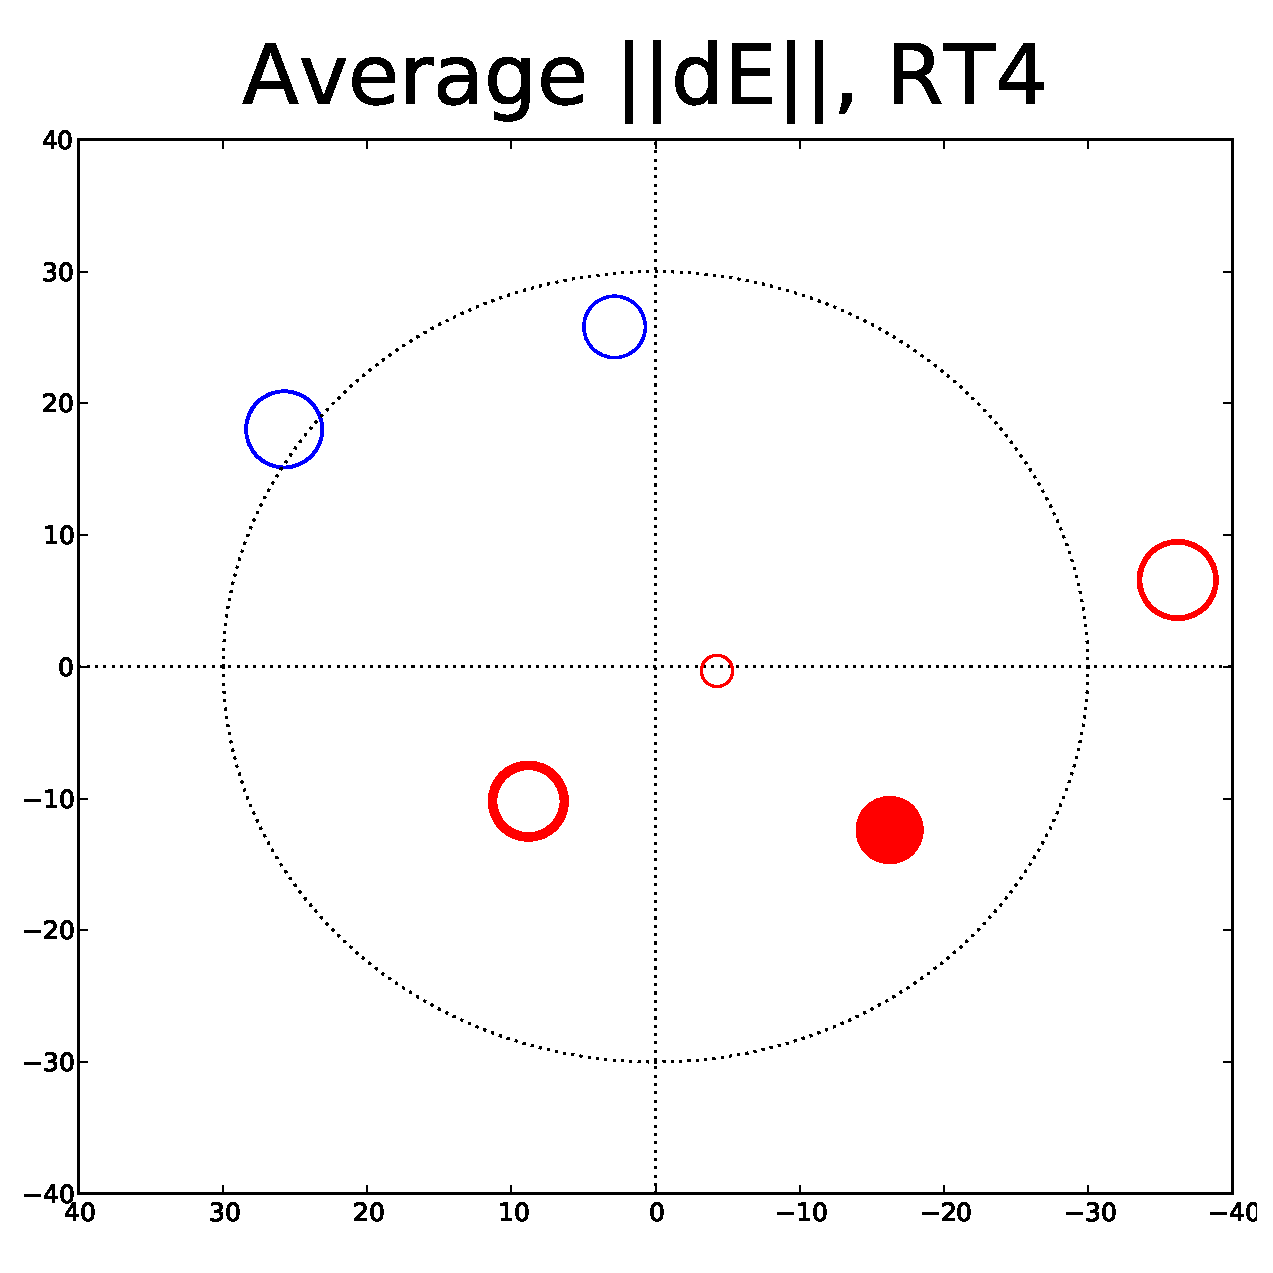
\includegraphics[width=\roguewidth]{o2006_dE_ant4} \\
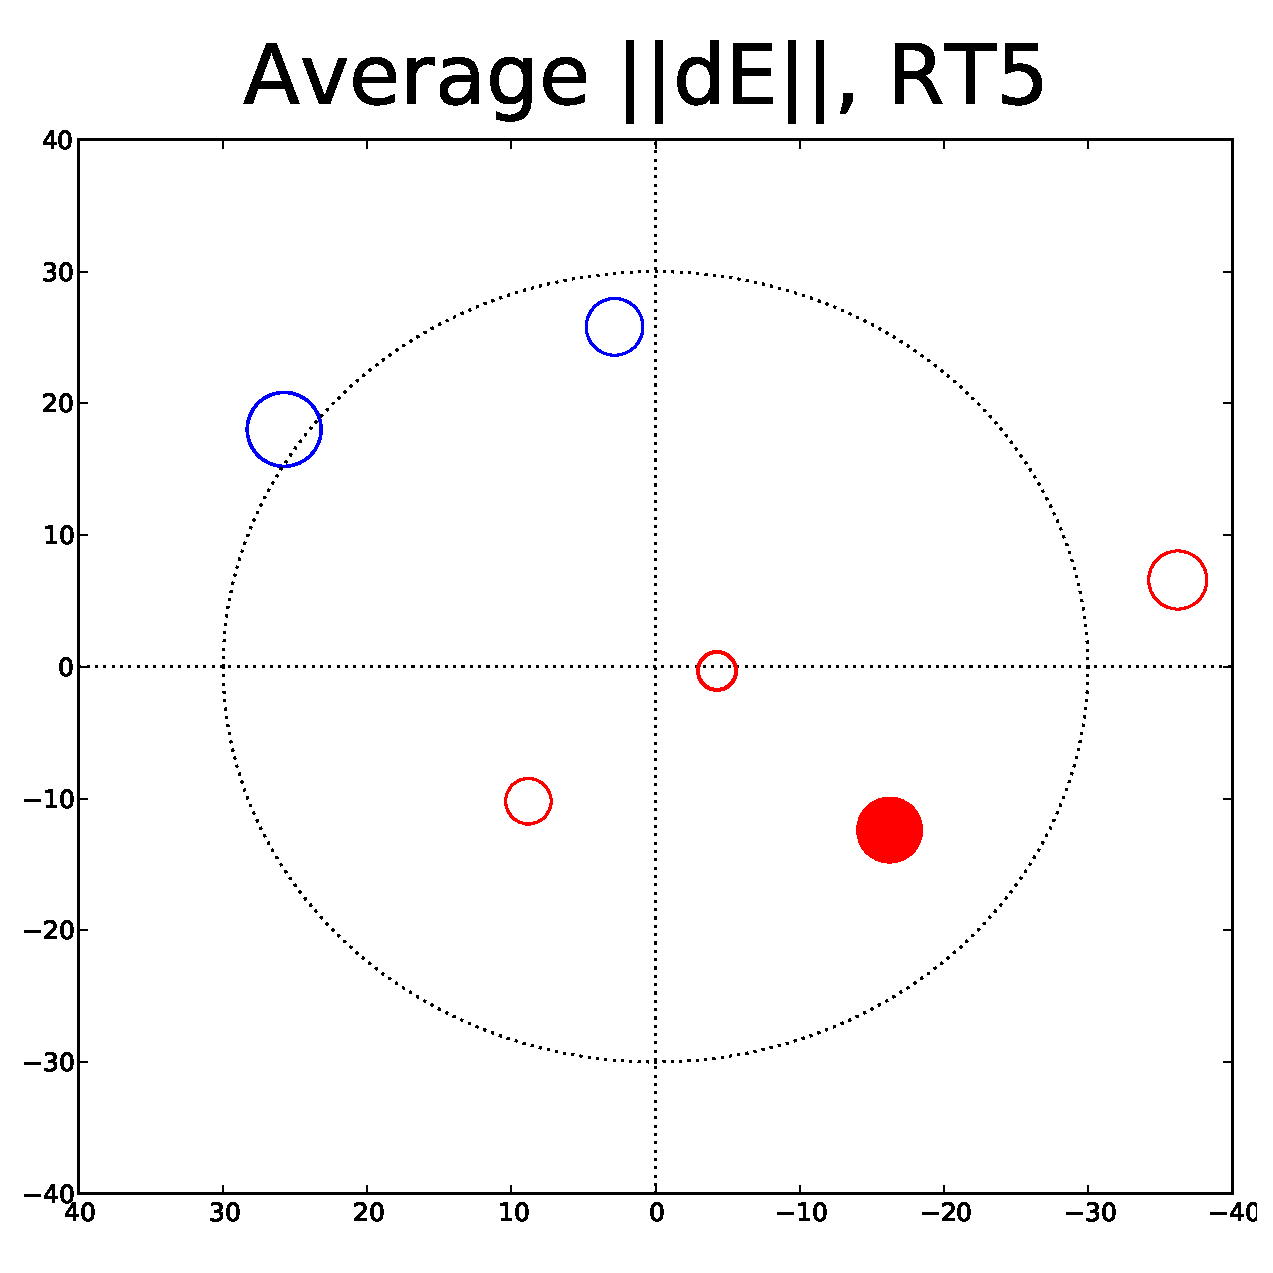
\includegraphics[width=\roguewidth]{o2006_dE_ant5} &
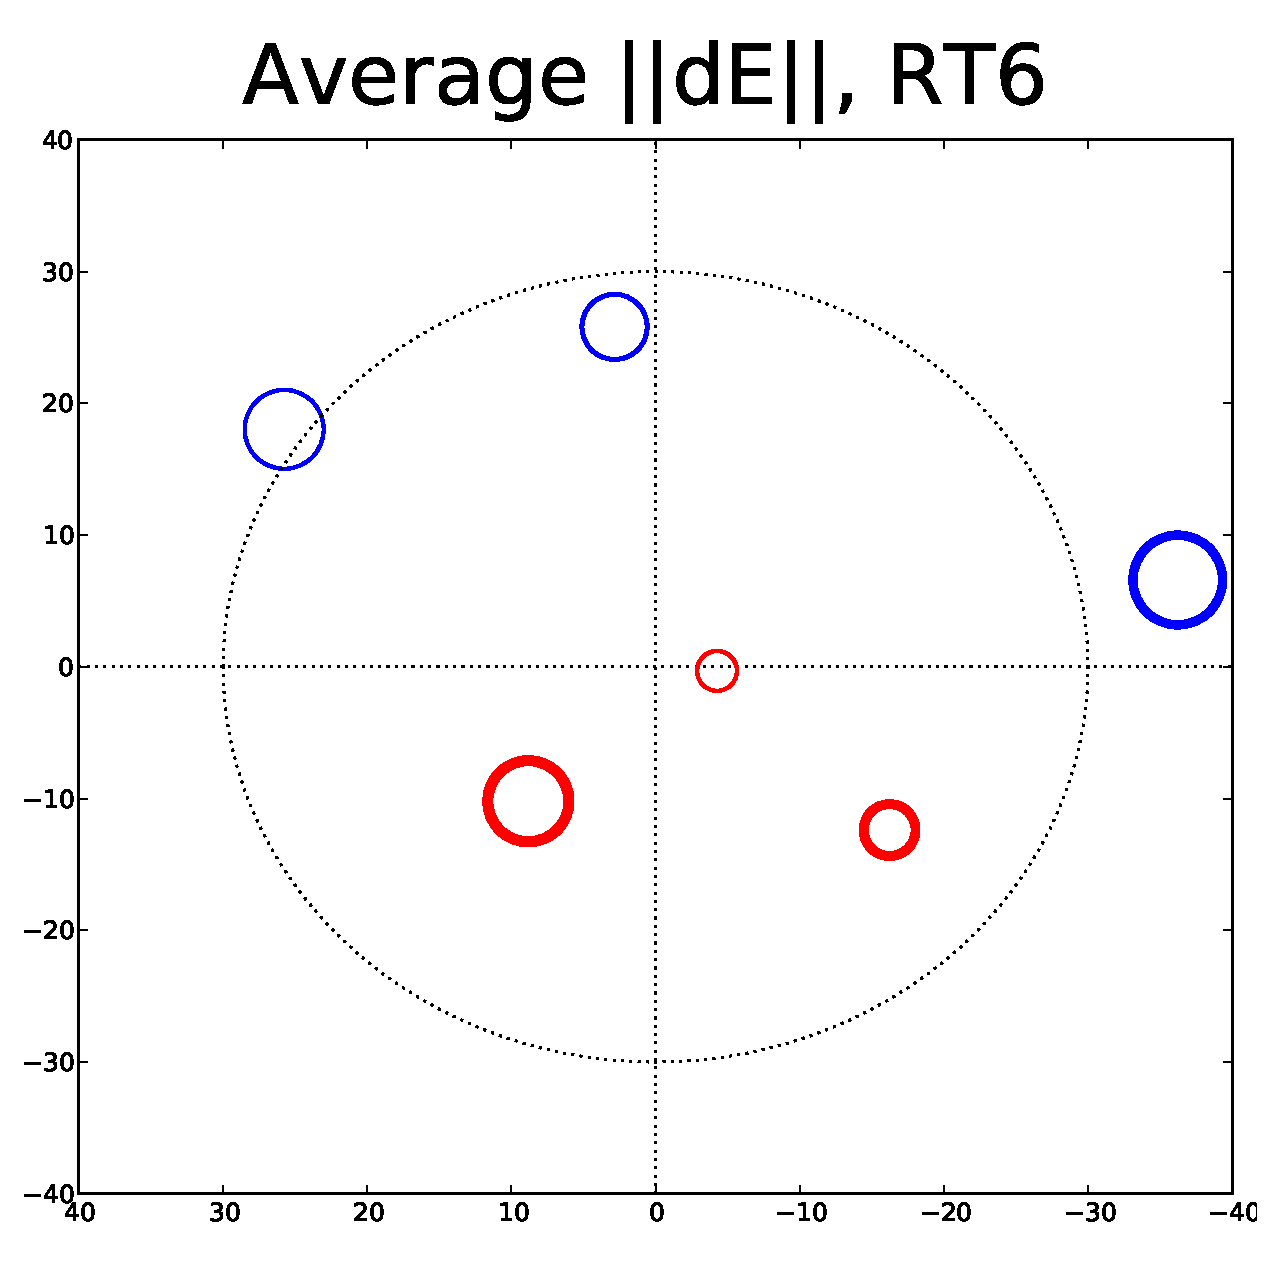
\includegraphics[width=\roguewidth]{o2006_dE_ant6} &
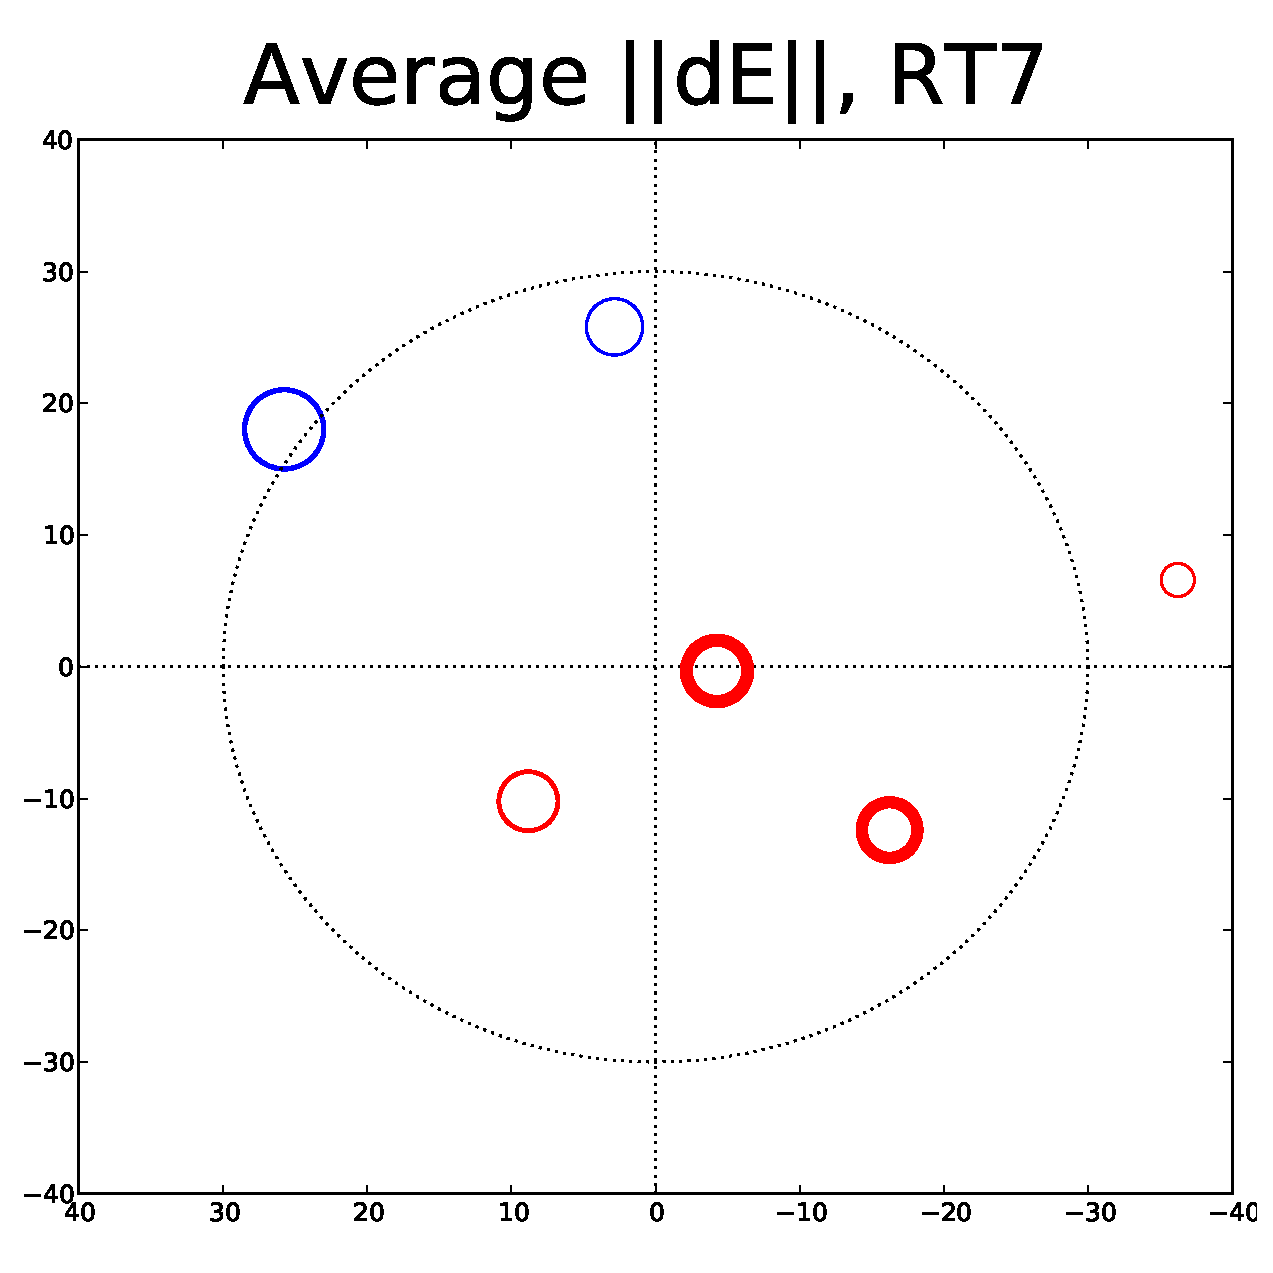
\includegraphics[width=\roguewidth]{o2006_dE_ant7} &
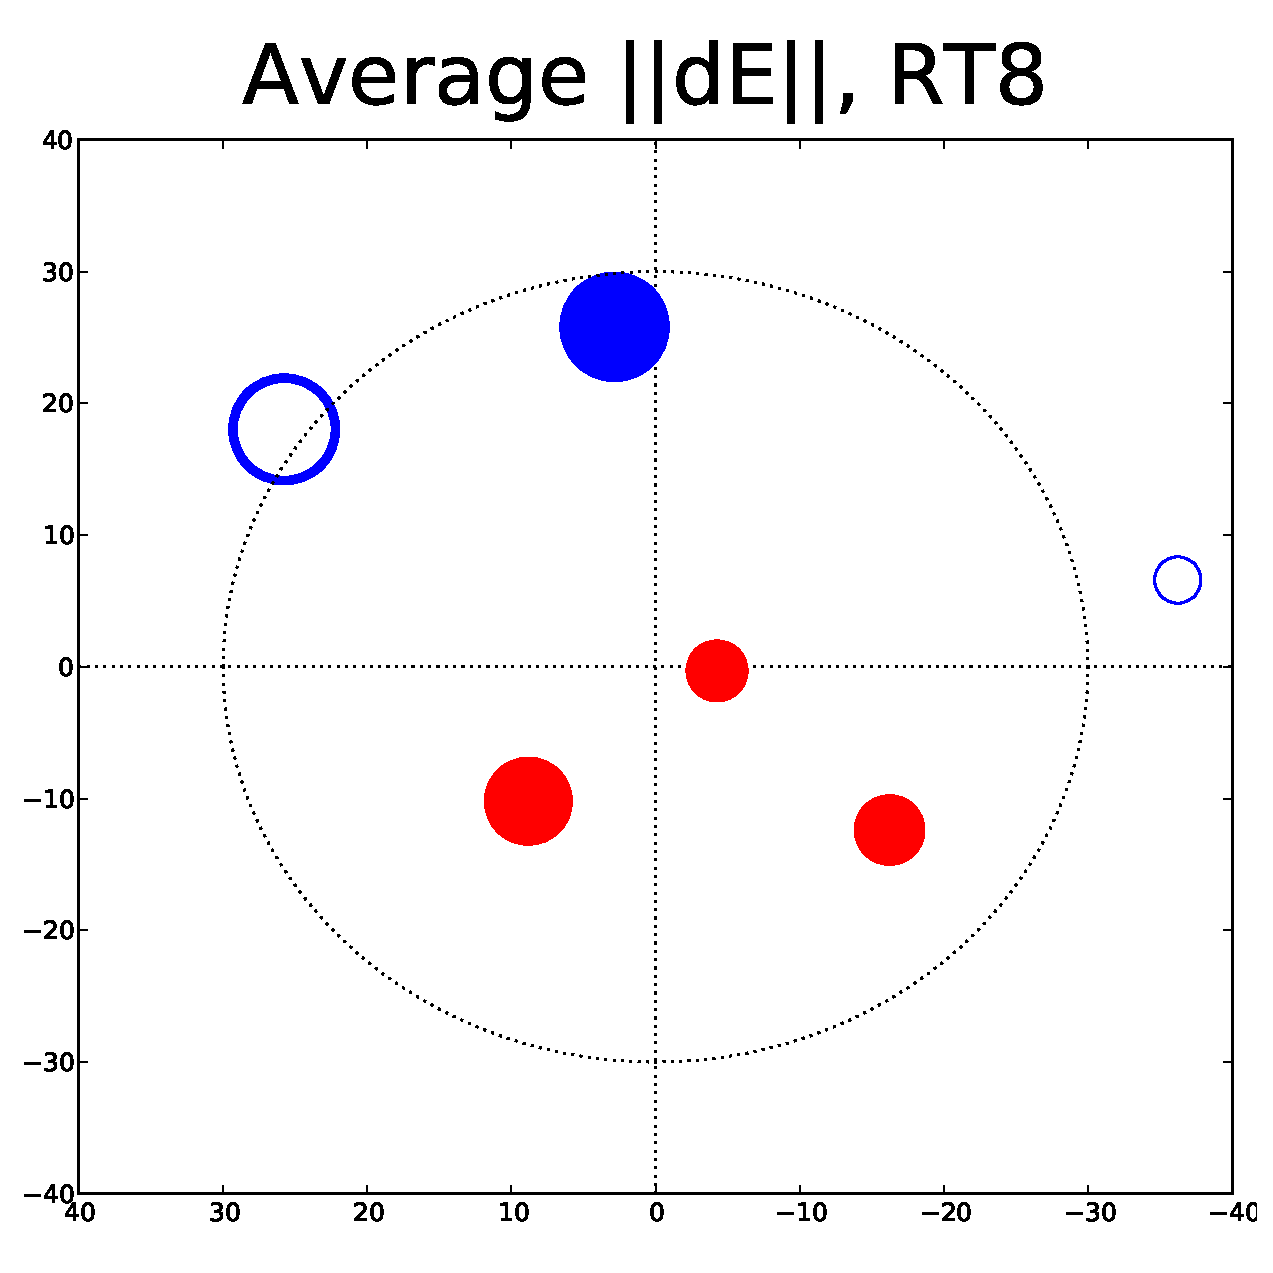
\includegraphics[width=\roguewidth]{o2006_dE_ant8} &
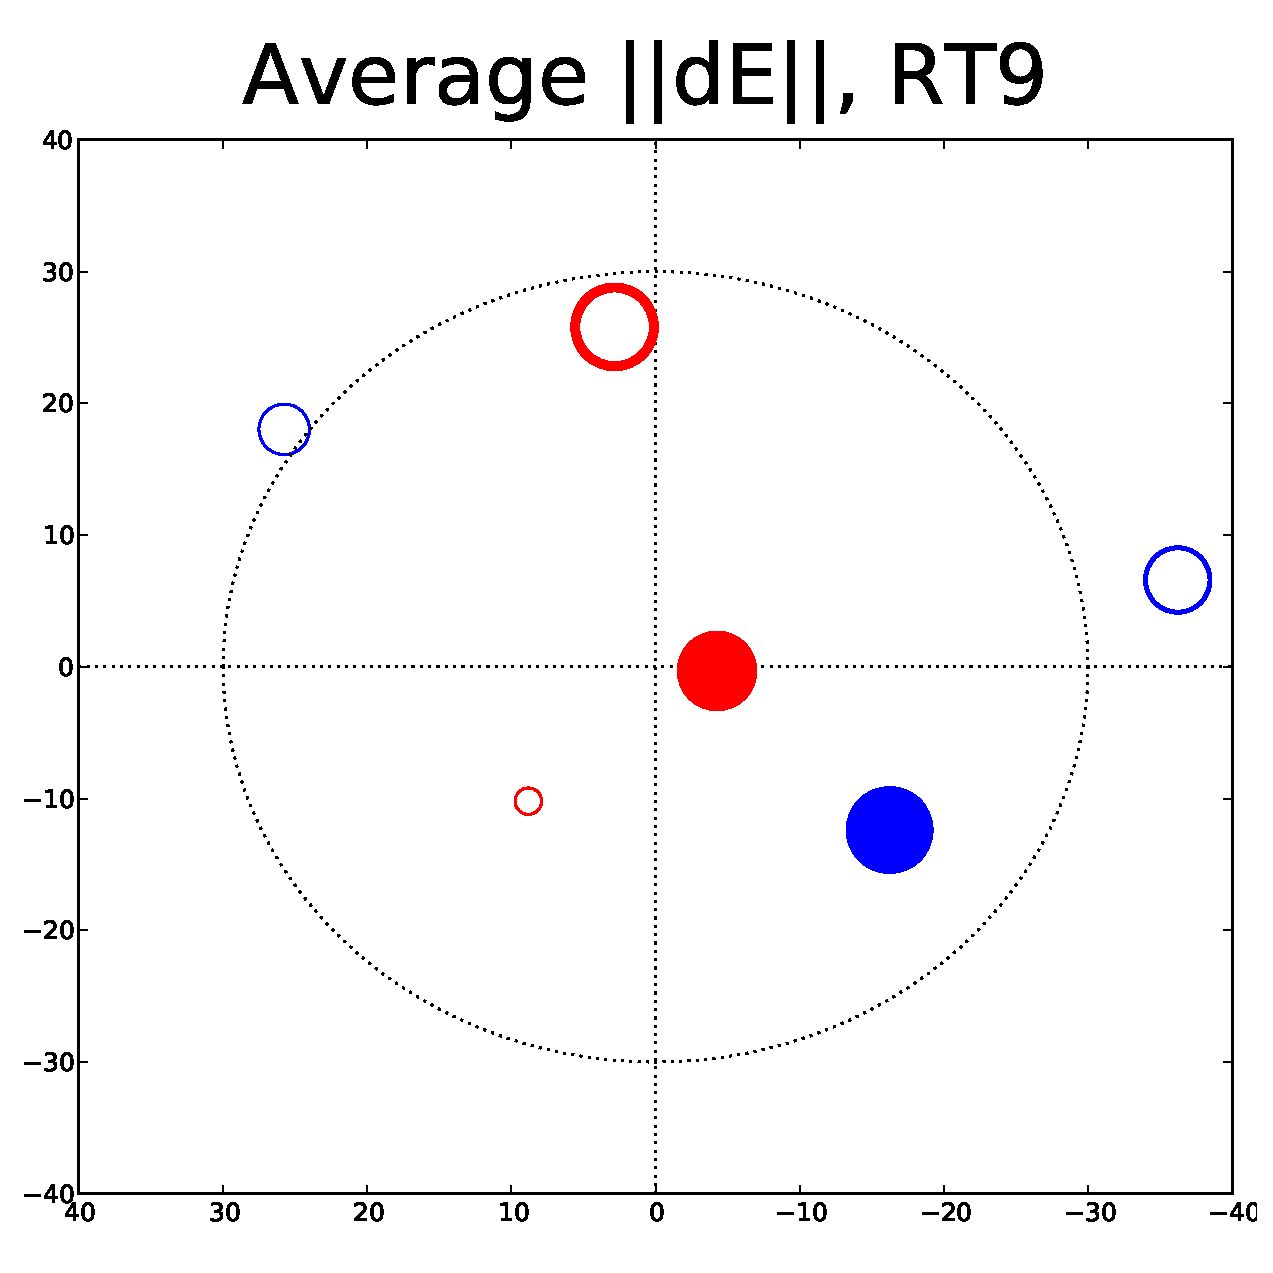
\includegraphics[width=\roguewidth]{o2006_dE_ant9} \\
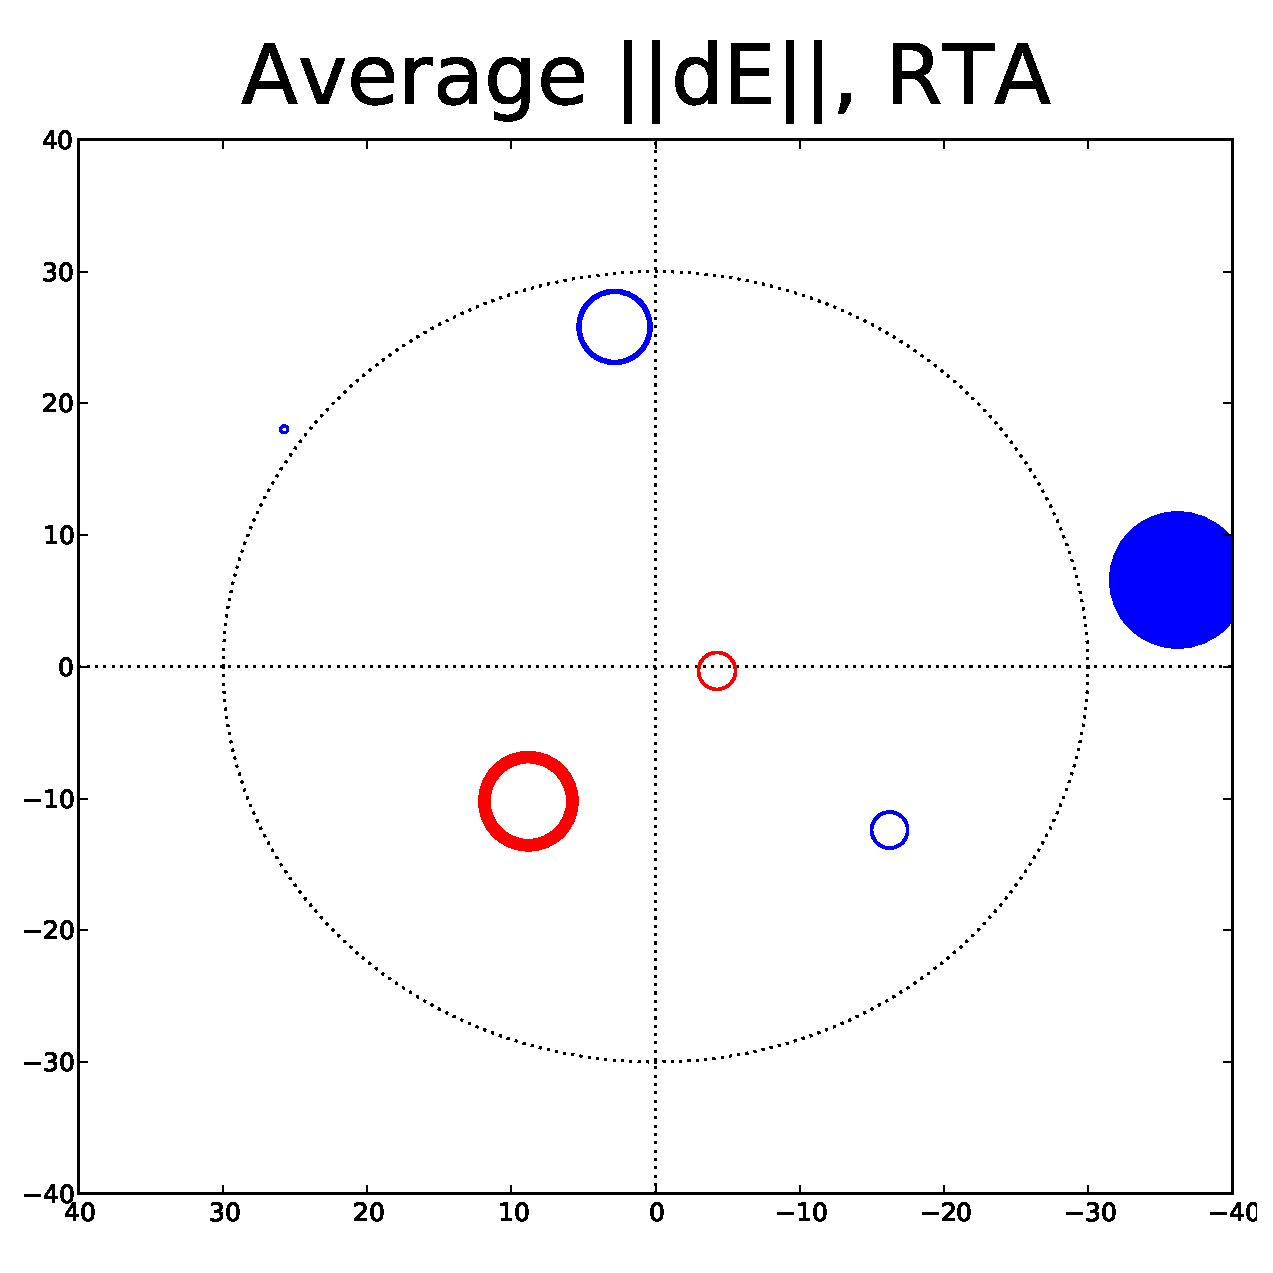
\includegraphics[width=\roguewidth]{o2006_dE_antA} &
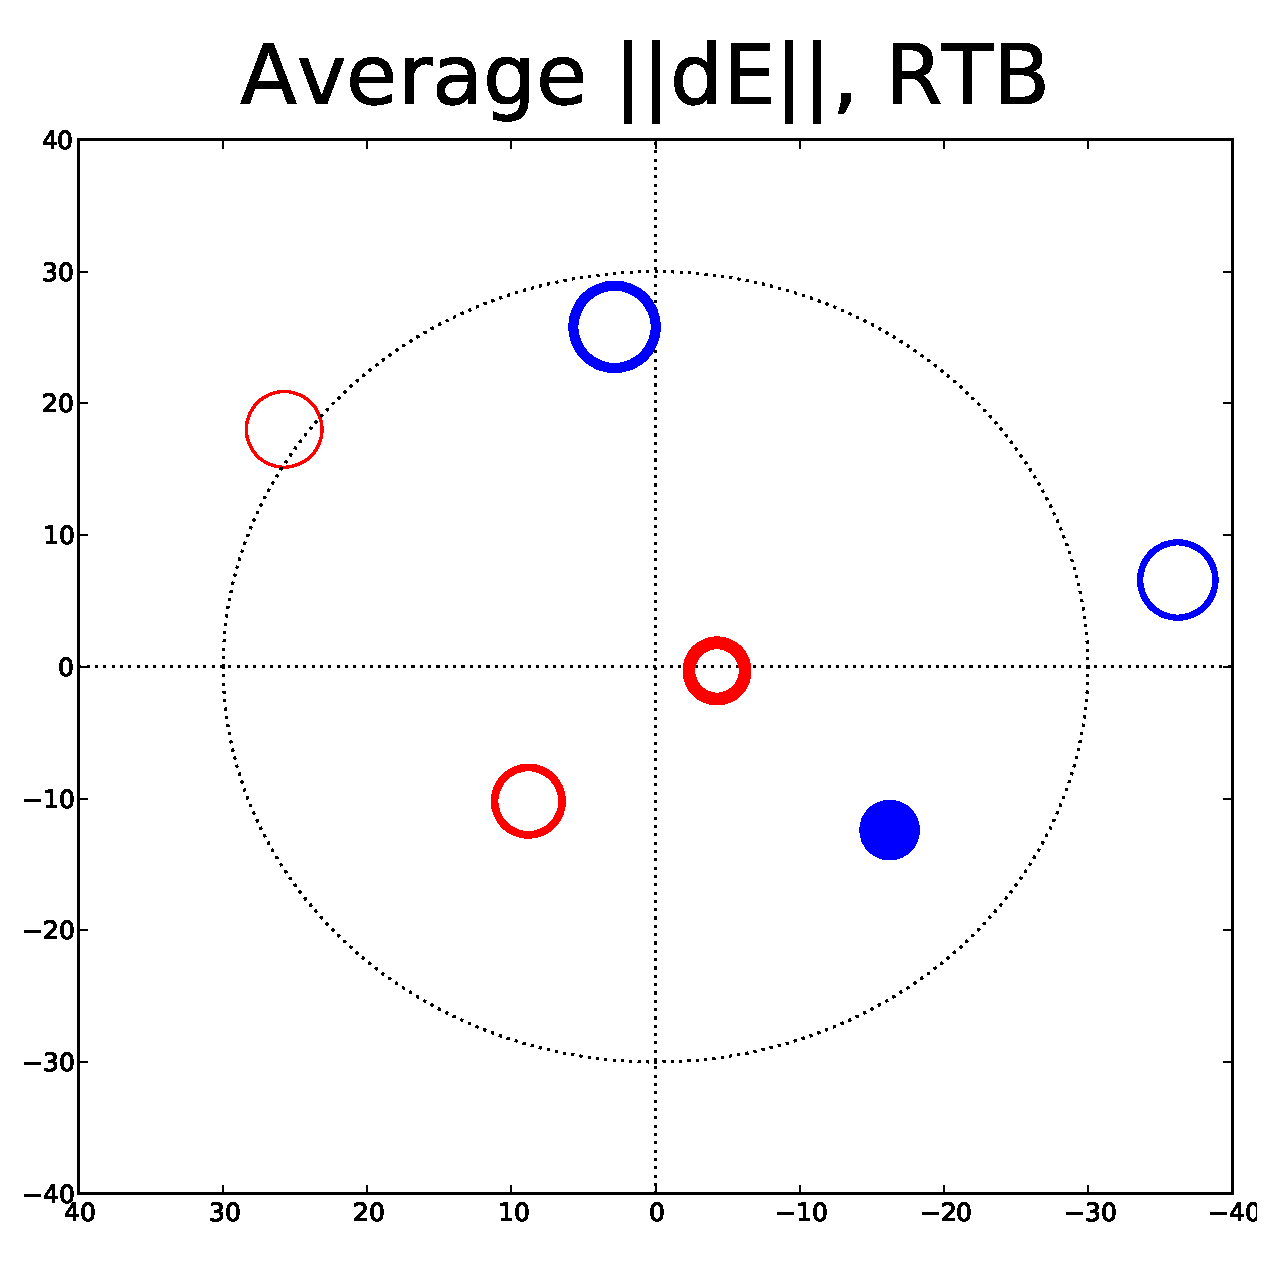
\includegraphics[width=\roguewidth]{o2006_dE_antB} &
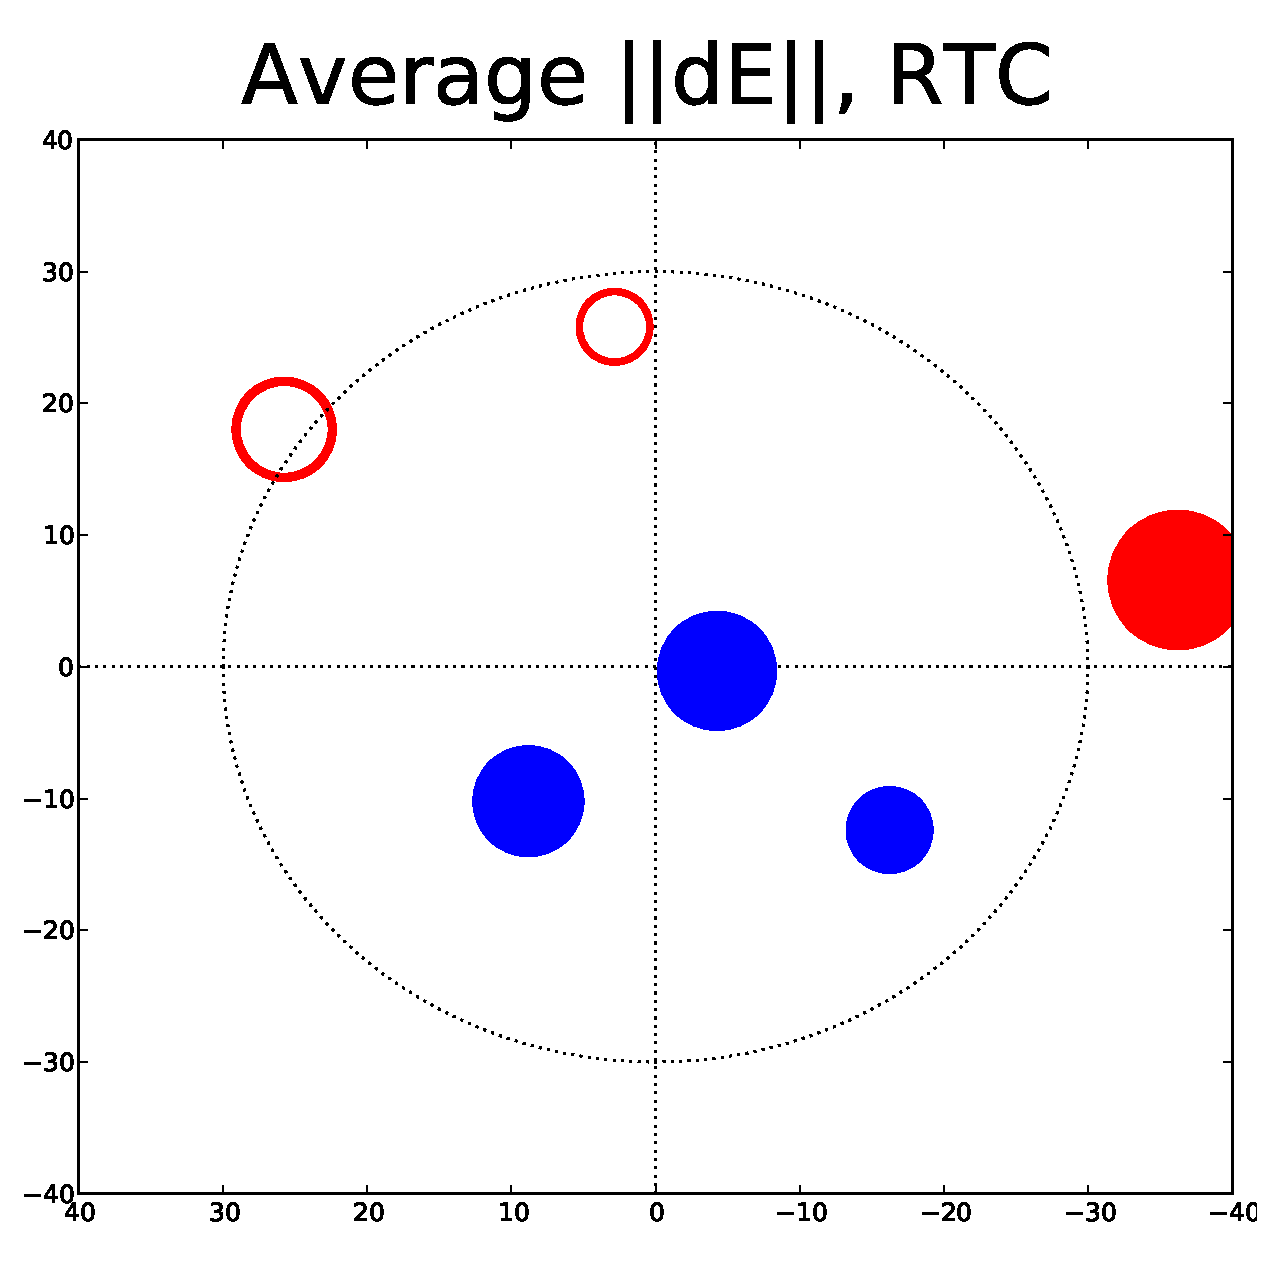
\includegraphics[width=\roguewidth]{o2006_dE_antC} &
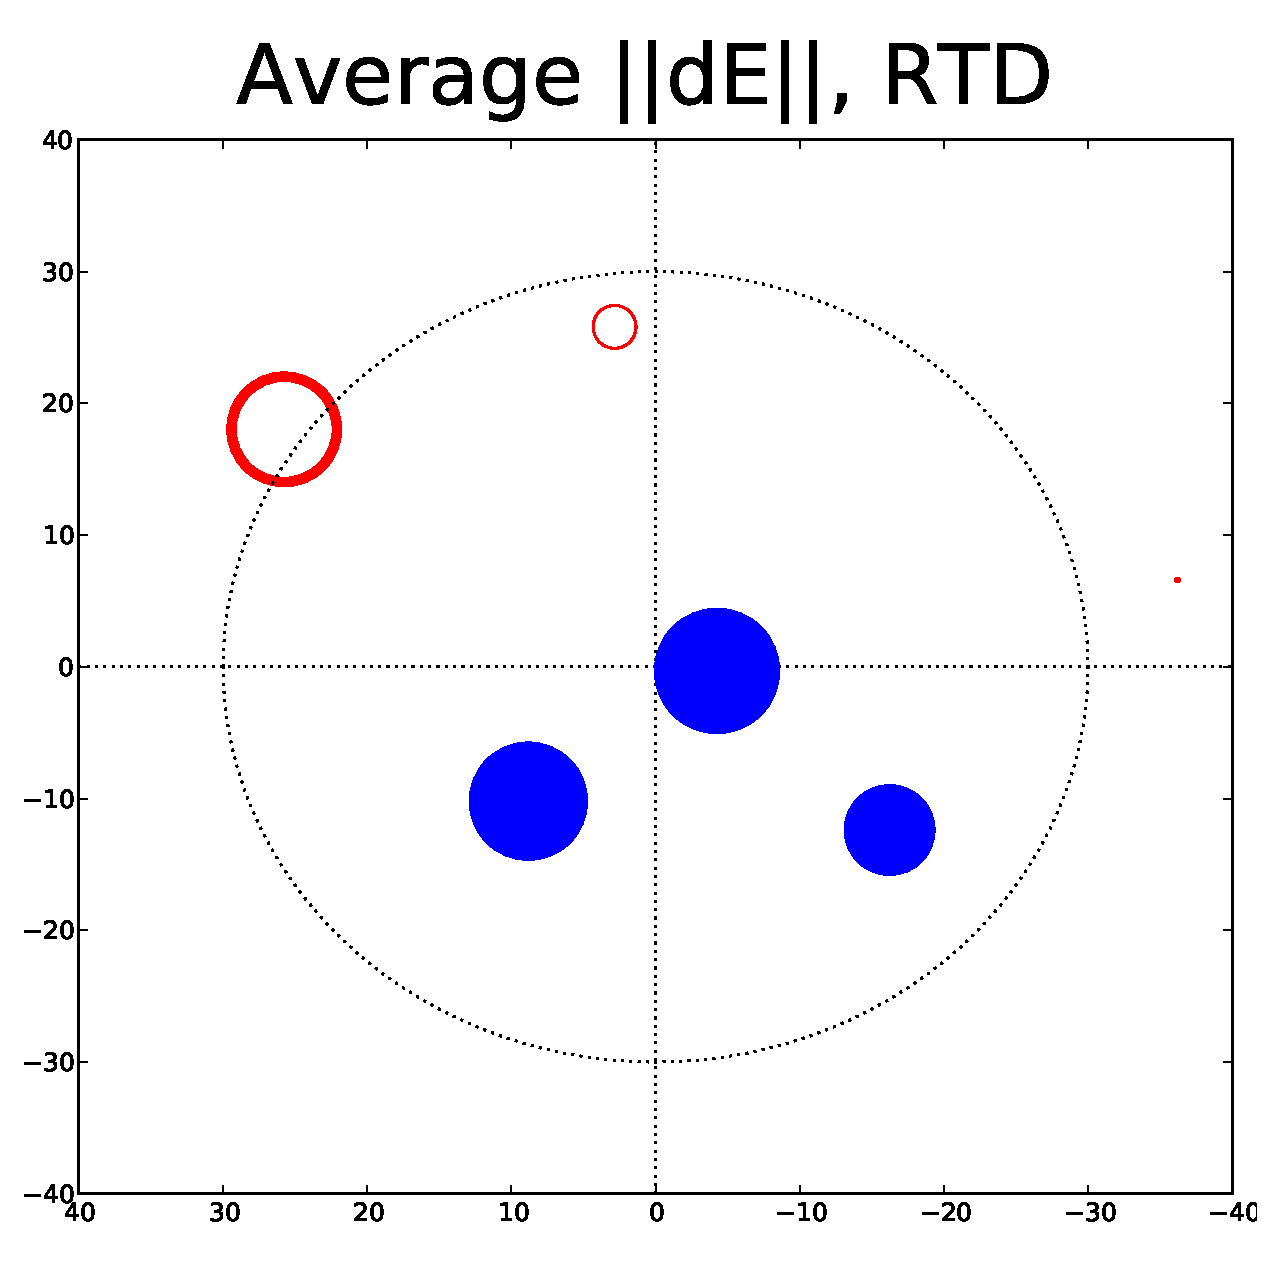
\includegraphics[width=\roguewidth]{o2006_dE_antD} 
\end{tabular}
\caption{\label{fig:rogues-2006}``Rogues gallery'' plot for the 2006 observation, using the same scale as Fig.~\ref{fig:rogues-2003}}
\end{figure}


The galleries show exactly such a pattern for antennas RT5 through RT8 (and perhaps RT4), for both the 2003 and, to a lesser extent, the 2006 observations. It is a little bit strange that 4 (or even 5) adjacent antennas would so consistently mispoint North, and do the same three years later. Perhaps this is another, poorly understood consequence of unmodelled source structure. Some pointers to this are that antennas RT4--8, being in the middle of the array, form up predominantly shorter baselines, and that the long-baseline antennas RTC and RTD exhibit the opposite behaviour. (What hinders such an analysis is the unfortunate fact that the three brightest off-axis sources all exhibit some structure, and all three lie in the bottom half of the field.) Another puzzling feature is the consistently low $||\Delta\jones{E}{}||$ for sources F, H and K on antenna RTC in 2003 (and to a far lesser extent in 2006). If due to source structure, why does it not repeat on RTD? Perhaps RTC is mispointing to the South?

Antennas RT0--2, RT9 and RTA, on the other hand, show completely different patterns, with little to no similarity between 2003 and 2006. Some of these are consistent with a static mispointing. Some antennas (RT8 and RT9, and RTB especially) also show a hint of time variability in $||\Delta\jones{E}{}||$.

In any case, it is clear that the complicated interaction between source structure and differential gain-amplitudes makes the latter extremely difficult to interpret. Note also that my (or rather de Bruyn's) source model was built by NEWSTAR based on regular selfcal, so there's bound to be some contamination from DDE-related artifacts in the source parameters. 
Truly robust methods for disentangling source structure from DDEs have yet to be developed. \EDIT{It is also clear that an approach that parameterizes the DDEs in a ``global'' way, such as pointing selfcal, is the way forward -- what is not yet clear is how much the global solution itself can be affected by unmodelled structure in the brighter sources, and what to do about it.}

\subsection{Phase behaviour}

%for t in o2003 o2006; do plot-de-solutions.py --phase-slope -o eps -r --portrait --title-fontsize 0 -W 290 -H 40 --borders 0.03,1.12,0.03,1.5 --circle-borders 0.05,0.99,0.05,0.99 $t.cache --phase-slope-dlm --dlm-scale 1200 --subtitle-fontsize 10 --axis-fontsize 9 --circle-axis-fontsize 14 --circle-label-fontsize 20 --phase-slope-time-offset -0.096 --output-prefix $t --lsm 3C147.lsm.html --subplot-wspace 0.3 --radius 75; done

\begin{figure}
\centering
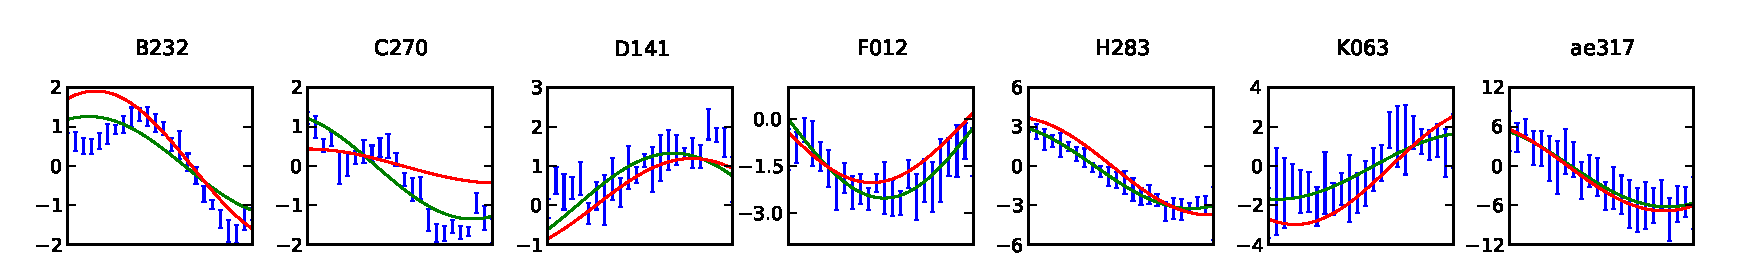
\includegraphics[width=\columnwidth]{o2003_dEphase_array_slopes}\\
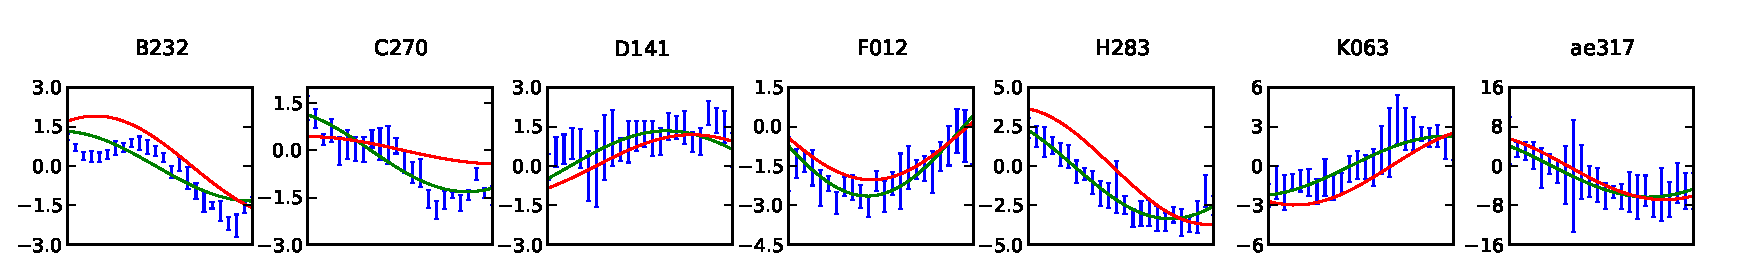
\includegraphics[width=\columnwidth]{o2006_dEphase_array_slopes}
\caption{\label{fig:dEphase-slope}Phase slopes over the array as a function of time (in deg/km) in the direction of the seven sources for the 2003 (top) and 2006 observations (bottom). The green lines indicate phase slopes corresponding to the fitted position offsets (Fig.~\ref{fig:dEphase-dlm}), the red lines -- phase slopes corresponding to an overall field rotation of $45\arcsec$.}
\end{figure}

\begin{figure}
\centering
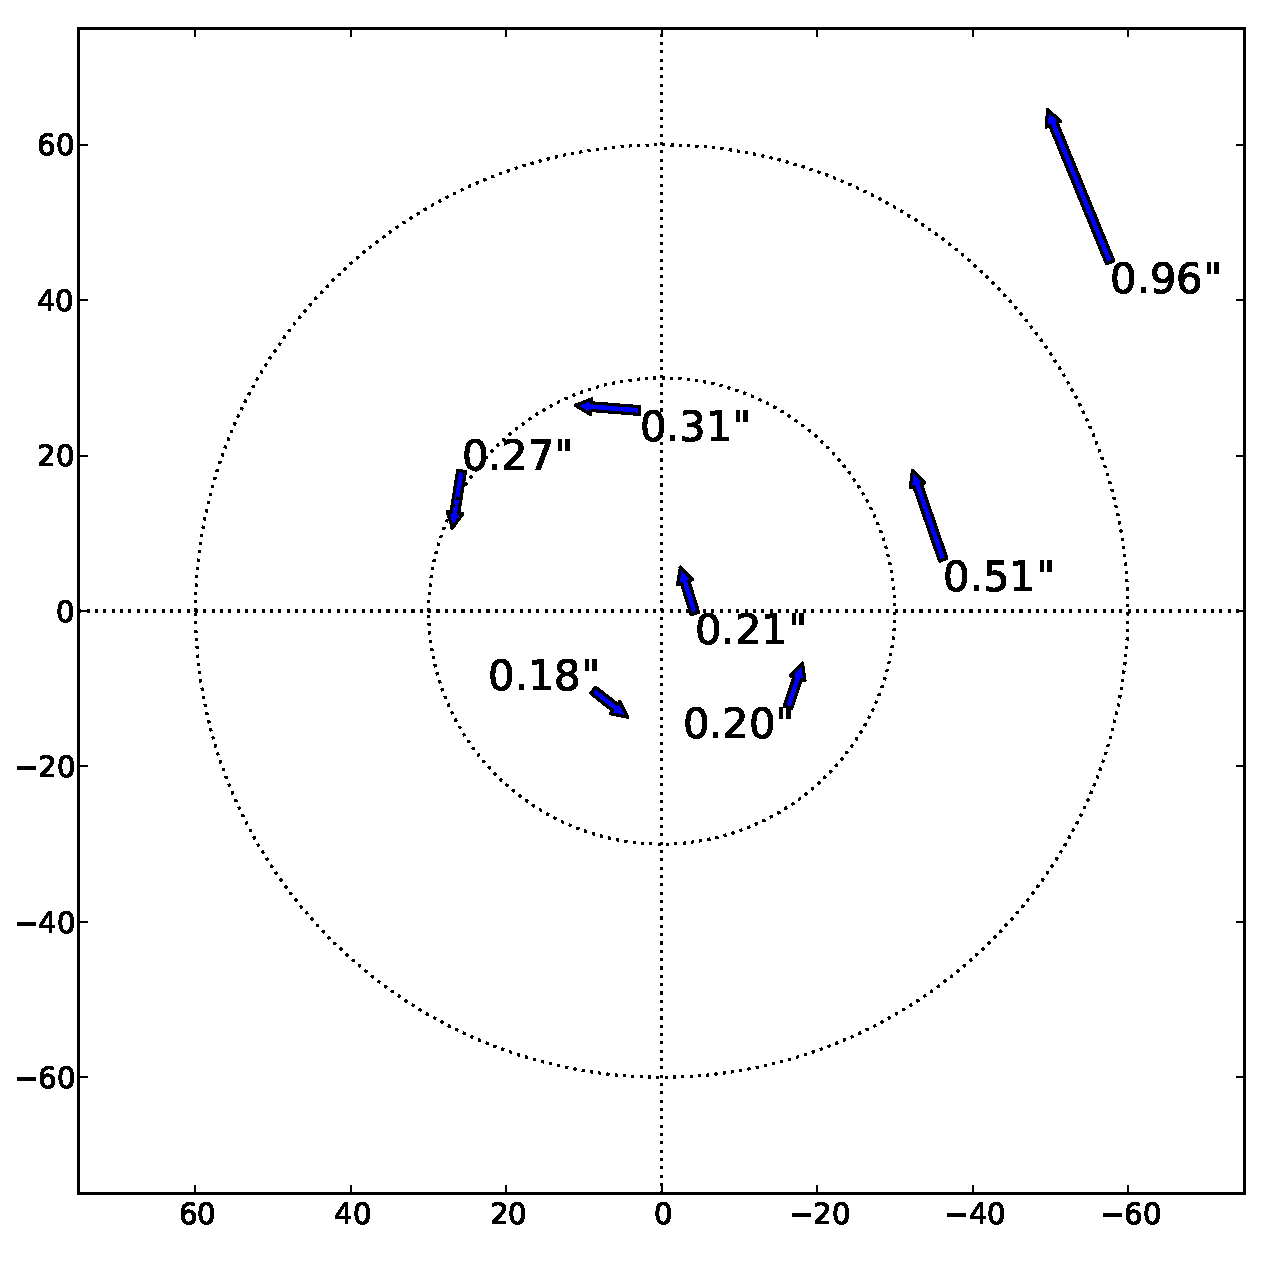
\includegraphics[width=.5\columnwidth]{o2003_dE_lm_offsets}%
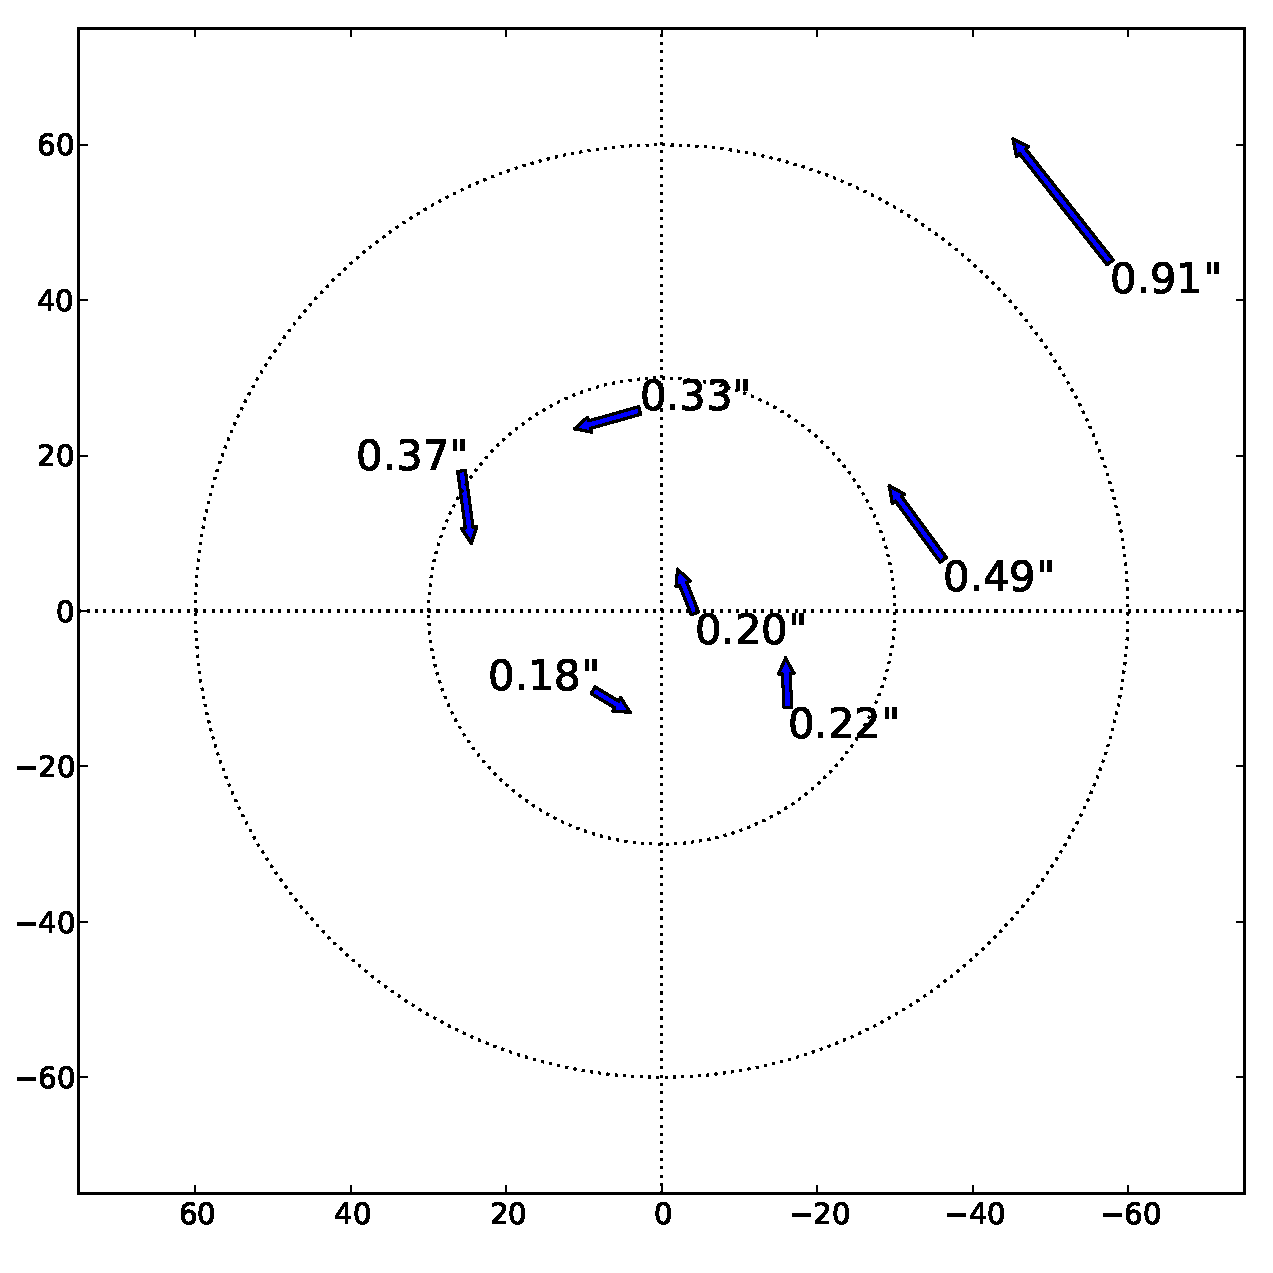
\includegraphics[width=.5\columnwidth]{o2006_dE_lm_offsets}\\
\caption{\label{fig:dEphase-dlm}Fitted position offsets corresponding to the phase slopes of Fig.~\ref{fig:dEphase-slope} (2003 observation on the left, 2006 on the right). The length of the arrows is exaggerated by a factor of 1200: the biggest offset is in fact just under $1\arcsec$.}
\end{figure}

A rather prominent feature of the phase plots in Fig.~\ref{fig:dEphase} is their continuity from antenna to antenna, and the fact that the phases at the two ends of the array exhibit opposite temporal trends. This is suggestive of an evolving phase slope over the array. Fitting such a slope (per source) produces some very striking results (Fig.~\ref{fig:dEphase-slope}). The dominant phase effect is clearly global rather than antenna-based, and is extremely consistent across both observations.

A phase slope over the array can be interpreted as an apparent position offset. It appears that the slope behaviour in Fig.~\ref{fig:dEphase-slope} can be fitted quite well by \emph{constant} position offsets. 
The best-fitting position offsets are indicated in Fig.~\ref{fig:dEphase-dlm}, and the corresponding slope curves are plotted in green on Fig.~\ref{fig:dEphase-slope}. 

Figure~\ref{fig:dEphase-dlm} immediately suggests a field rotation. And indeed, the entire collection of phase slopes (for both the 2003 and 2006 observation), is, to first order, consistent with a rotation of $45\arcsec$ around the phase centre. The corresponding slope curves are plotted in red. While there are some significant differences in the brighter sources, it seems clear that the dominant effect is not an instrumental DDE at all, but a systematic rotation of the sky model. The model positions are derived by NEWSTAR from direct fits to the visibilities, and de Bruyn (priv. comm.) has independently cross-checked the positions of distant sources against the NVSS, which seems to preclude a rotation in the model itself. Note that a $45\arcsec$ rotation can also be introduced by a clock error of about 2.9 s, or a corresponding rotational error in conversion of UVW coordinates from apparent to J2000. Since NEWSTAR and MeqTrees use completely different toolchains and visibility data formats, I cannot exclude a coordinate conversion error somewhere along the line. This needs to be urgently investigated. If indeed the entire sky model is slightly rotated, then perhaps the image of Fig.~\ref{fig:3C147} can even be improved upon!

\subsection{Feeding differential gains back into the sky model\label{sec:model-improvement}}

The results above suggested that I could improve my sky model by feeding back in some information extracted from the $\Delta\jones{E}{}$ solutions. In the previous section, I obtained a correction to the model positions of the seven sources.\footnote{For the moment, I've left aside the issue of whether the positional offsets are ultimately due to a global field rotation. Improving the positions of seven of the brightest off-axis sources should already produce an superior sky model.} Following the discussion of Sect.~\ref{sec:de-analysis-model}, I could also provide corrections for the $I$ and $Q$ fluxes by applying the per-source average $\Delta\jones{E}{}$ amplitudes:

\begin{eqnarray*}
\coh{B}{s}^\mathrm{(corr)} & = & \overline{|\Delta\jones{E}{s}|} \coh{B}{s} \overline{|\Delta\jones{E}{s}|} \\
\overline{|\Delta\jones{E}{s}|} & \equiv & \matrixtt{\overline{|\Delta e_{xs}|}}{0}{0}{\overline{|\Delta e_{ys}|}} = \frac{1}{N_\mathrm{ant}N_t N_\nu} \sum_{p,i,j} |\Delta\jones{E}{sp}(t_i,\nu_j)|,
\end{eqnarray*}

where $t_i$ and $\nu_j$ represent the time and frequency solution intervals of $\Delta\jones{E}{}$. In terms of the $I$ and $Q$ fluxes, the correction becomes:

\begin{eqnarray*}
I^\mathrm{(corr)} = \Sigma \cdot I + \Delta \cdot Q, & \; &  Q^\mathrm{(corr)} = \Delta \cdot I + \Sigma \cdot Q, \\
\Sigma = \frac{1}{2}\left( \overline{|\Delta e_{xs}|}^2 + \overline{|\Delta e_{ys}|}^2 \right), 
& \; & \Delta = \frac{1}{2}\left( \overline{|\Delta e_{xs}|}^2 - \overline{|\Delta e_{ys}|}^2 \right).
\end{eqnarray*}

I therefore applied these corrections for $I$, $Q$, and position to my sky models (independently for the 2003 and 2006 observations), and repeated the calibration procedure. An improvement in single-band residuals was immediately apparent (Fig.~\ref{fig:residuals-newmodel}) -- after $\jones{G}{p}$ and $\coh{M}{pq}$ solutions, the seven off-axis sources subtracted noticeably better. Residuals after $\Delta\jones{E}{sp}$ solutions, on the other hand, looked pretty much the same (this is not surprising, since differential gains had already taken care of the visible off-axis errors in the original reduction), with a very slight improvement around 3C147 itself. 
which can be explained by improved $\jones{G}{p}$ solutions due to the more accurate sky model.

\begin{figure}
\begin{centering}
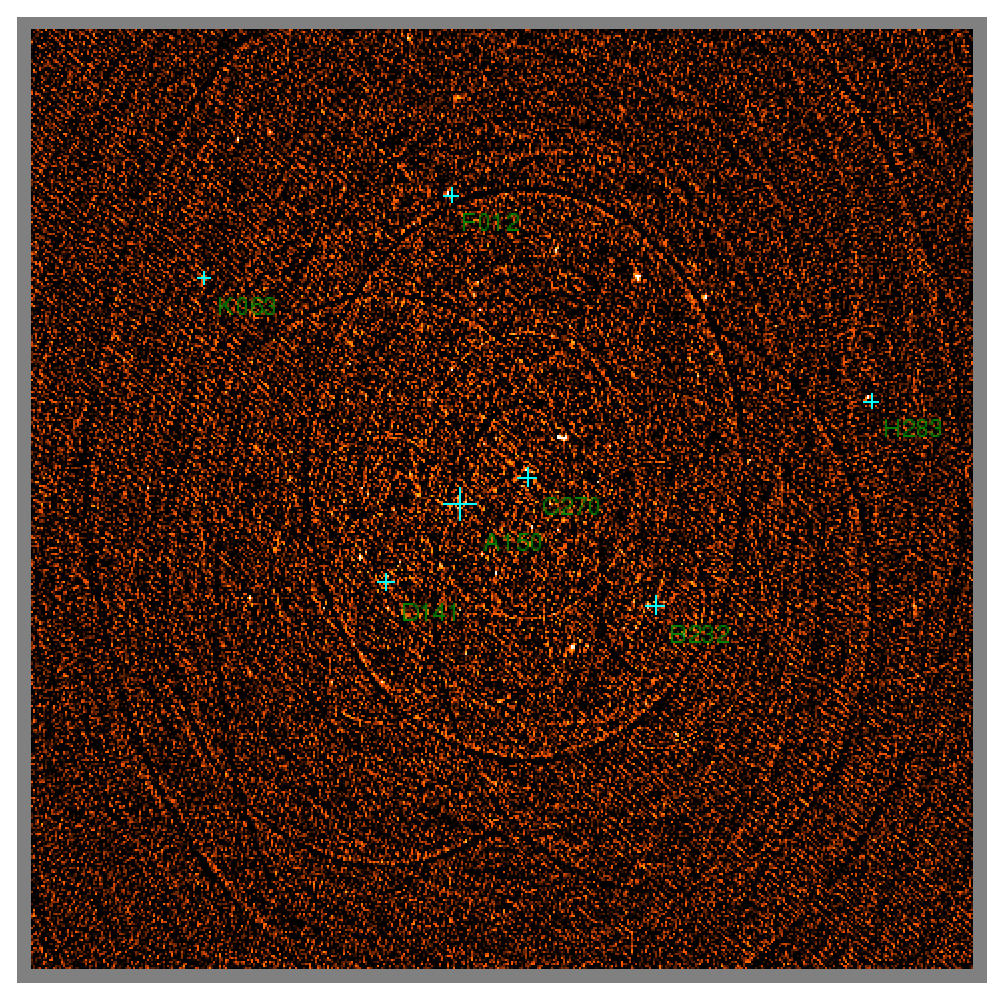
\includegraphics[width=.5\columnwidth]{spw2_oldmodel}%
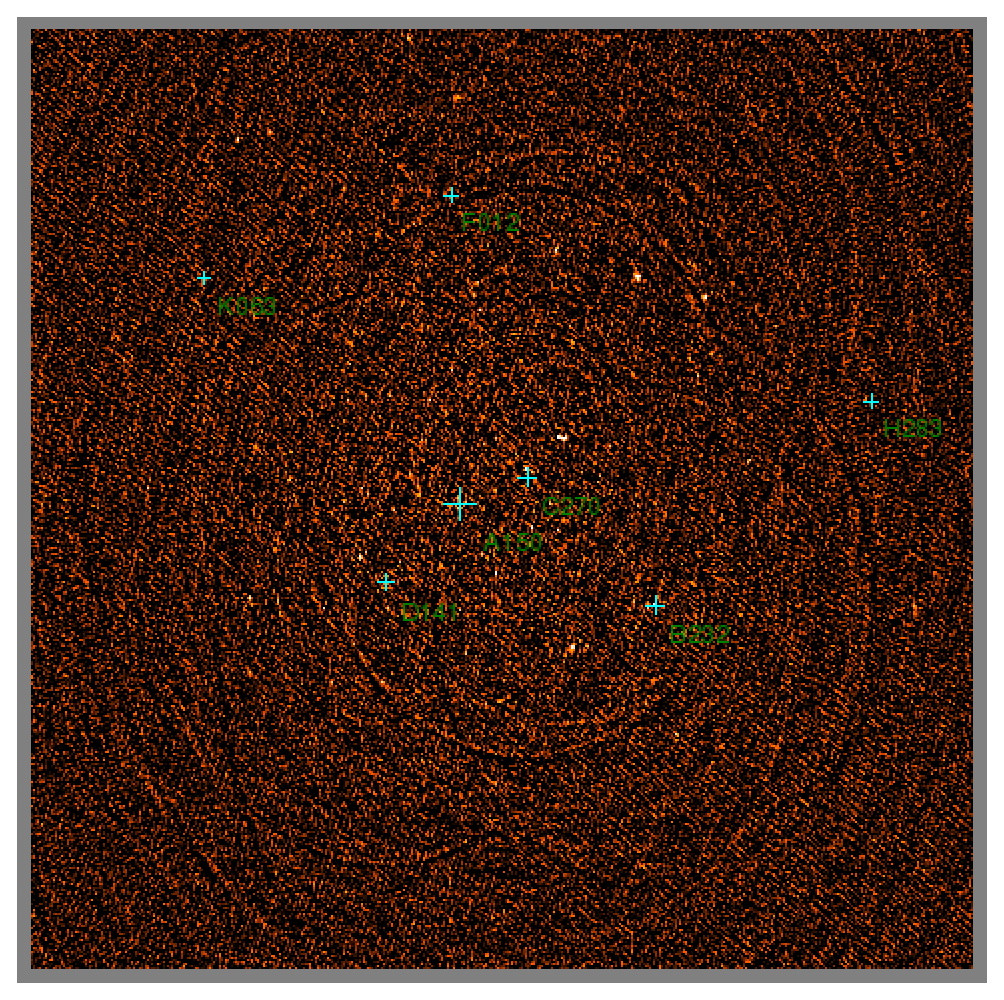
\includegraphics[width=.5\columnwidth]{spw2_newmodel}\par
\end{centering}
\caption{\label{fig:residuals-newmodel}Calibration with an improved sky model. This shows single-band residual images after $\jones{G}{p}$ and $\coh{M}{pq}$ solutions. The left image is from the original reduction, the right image uses a sky model improved via my $\Delta\jones{E}{}$ analysis. Crosses indicate the positions of sources for which the model was improved, plus 3C147 itself (source A).}
\end{figure}

\subsection{Phase behaviour II\label{sec:de-analysis-phase2}}

Presumably, the remaining residual structures in Fig.~\ref{fig:residuals-newmodel} are more representative of the instrumental DDEs per se, since inaccuracies in the sky model have been significantly reduced. We should also expect the differential gain solutions to be more indicative of the actual DDEs (apart from the issue of resolved sources affecting $||\Delta\jones{E}{}||$ on antennas RTC and RTD, which the improved sky models do not address at all). Of particular interest is the effect that the improved model has on the differential gain-phases. As for the gain-amplitudes, we would expect them to differ by only an overall per-source scaling factor. Indeed, making the same $||\Delta\jones{E}{}||$ plot as in Fig.~\ref{fig:dEampl} confirms this -- it is, to all intents and purposes, identical (and omitted here to save space), since the plotted amplitudes are renormalized by the per-source average $||\Delta\jones{E}{}||$.

\begin{figure*}
\sidecaption
\parbox[b]{12cm}{
\includegraphics[width=12cm]{o2003new_dEphase_mean}
\includegraphics[width=12cm]{o2006new_dEphase_mean}
}
\caption{\label{fig:new-dEphase}Differential gain-phases ($\arg\Delta\jones{E}{}$, in degrees) as a function of time, using improved sky models for the 2003 (top) and 2006 (bottom) observations. Compare to Fig.~\ref{fig:dEphase}.}
\end{figure*}

The phases, on the other hand, show a marked difference, since the formerly dominant effect -- that of position offsets -- has been taken out. The $\arg\Delta\jones{E}{}$ solutions themselves are shown in Fig.~\ref{fig:new-dEphase}. Phase slopes are still very much in evidence, as can be seen in Fig.~\ref{fig:new-dEphase-slope}. Somewhat surprisingly, these slopes indicate that some residual position offsets remain, at a level of 15\% to 20\% of the original offsets (Fig.~\ref{fig:new-dEphase-dlm}). This suggests that my procedure of fitting phase slopes to $\arg\Delta\jones{E}{}$ solutions, followed by fitting position offsets to the slopes, systematically \emph{underestimates} the true position offsets. This is possibly an effect of the complex averaging implicit in having one $\Delta\jones{E}{}$ solution per a relatively large solution interval (20 MHz by 30 minutes). If so, this could perhaps be incorporated as a multiplicative correction factor in the model update procedure. Further work is required to fully understand the effect. 

%for t in o2003new o2006new; do plot-de-solutions.py --phase-slope -o eps -r --portrait --title-fontsize 0 -W 290 -H 40 --borders 0.03,1.12,0.03,1.5 --circle-borders 0.05,0.99,0.05,0.99 $t.cache --phase-slope-dlm --dlm-scale 1200 --subtitle-fontsize 10 --axis-fontsize 9 --circle-axis-fontsize 14 --circle-label-fontsize 20 --output-prefix $t --lsm $t-3C147.lsm.html --subplot-wspace 0.3 --radius 75; done

\begin{figure}
\centering
\includegraphics[width=\columnwidth]{o2003new_dEphase_array_slopes}\\
\includegraphics[width=\columnwidth]{o2006new_dEphase_array_slopes}
\caption{\label{fig:new-dEphase-slope}Phase slopes over the array as a function of time (in deg/km), using improved sky models for the 2003 (top) and 2006 observations (bottom). The green lines indicate phase slopes corresponding to the fitted position offsets (Fig.~\ref{fig:new-dEphase-dlm}). Compare to Fig.~\ref{fig:dEphase-slope}.}
\end{figure}

\begin{figure}
\centering
\includegraphics[width=.5\columnwidth]{o2003new_dE_lm_offsets}%
\includegraphics[width=.5\columnwidth]{o2006new_dE_lm_offsets}
\caption{\label{fig:new-dEphase-dlm}Fitted position offsets corresponding to the phase slopes of Fig.~\ref{fig:new-dEphase-slope} (2003 observation on the left, 2006 on the right). The length of the arrows is exaggerated by a factor of 1200: the biggest offset is in fact just under $0.2\arcsec$. Compare to Fig.~\ref{fig:dEphase-dlm}.}
\end{figure}

The brighter sources B, C, and (to a lesser extent) D show clear second-order phase effects, both in the phase slopes, and in the phase solutions themselves. The temporal continuity in the phase slopes can be interpreted as a \emph{time-variable} position offset. I can speculatively offer two explanations for such an offset:

\begin{itemize}
\item Unmodelled source structure (again!) For any given hour angle, an E-W array only sees an integrated cross-section through the source in a given direction. If the source is slightly resolved with an assymetric ``hotspot'', the zeroth-order moment of each such cross-section will be slightly different. 
\item Differential tropospheric or large-scale ionospheric refraction, including perhaps apparent change of baseline caused by refraction (the Anderson effect).
\end{itemize}

Another puzzling feature of the $\arg\Delta\jones{E}{}$ solutions in Fig.~\ref{fig:new-dEphase}
are the significant and (to first degree) constant phase offsets of some sources (e.g. H, K, ae) on some antennas. The offsets are mostly (though not completely) consistent between the 2003 and 2006 observations. None of the explanations offered above are consistent with a \emph{constant} phase offset! Could this be the phase component of the primary beam? There are too few sources in this reduction to infer any sort of directional dependence, but perhaps the ``QMC Project'' can provide more insights on this effect.

\subsection{The lurking errors\label{sec:deep-errors}}

The two calibrations (with the original and the improved sky models) described above have produced what appear to be identical final maps. This shows that the ``flyswatter'' can accomodate for significant errors in the sky model. On the other hand, the detailed structures in Fig.~\ref{fig:new-dEphase-slope} suggest that (even in the very benign case of 21 cm WSRT observations!) moderately bright off-axis sources still require some form of DDE correction even if the model is perfect. If this is the case, then a legitimate question is: why worry about getting the sky model right, if we need to do $\Delta\jones{E}{}$ solutions anyway, which will absorb any imperfections? (Besides the obvious caveats of the ``flyswatter'' discussed in Sect.~\ref{sec:dE-limitations}, that is.)

The rather striking image of Fig.~\ref{fig:diff-newmodel} shows that the final maps are not in fact identical, although the difference is buried in the noise. This image was produced by subtracting the original-model 8-band residual map from the improved-model map (2003 observation). 
Since the noise term in both maps is the same, subtraction reveals very faint structures that would normally be hidden in the noise. We're beginning to see more limitations of the ``flyswatter''. In the original reduction, apparent position offsets of the off-axis sources caused phase gradients in $t,\nu$-space in the differential gain-phases. These were approximated by a stepwise $\Delta\jones{E}{}$ solution (since I solved for only one $\Delta\jones{E}{}$ term per 30 minutes, per entire band), which proved to be good enough to drive off-axis errors to a level below the thermal noise. Improving the model positions has effectively ``flattened out'' these gradients, reducing the error made by a stepwise approximation even further. Figure~\ref{fig:diff-newmodel} demonstrates the improvement. The radial spokes correspond to ``jumps'' at the boundaries of the solution intervals, but the other structures (especially the half-circles) are rather more difficult to explain, and will have to be addressed in follow-up work.

\begin{figure}
\begin{centering}
\includegraphics[width=\columnwidth]{diff_newmodel_8band}%
\end{centering}
\caption{\label{fig:diff-newmodel}Calibration with an improved sky model. This shows the \emph{difference} between the 8-band residual maps (2003 observation) produced with the original and the improved sky models. Structures around 3C147 itself and the off-axis sources are mostly due to ``selfcal contamination'' in the original model caused by incorrect off-axis source positions. These are well within the noise: the intensity range of this image is $\pm2 \mu\mathrm{Jy}$, while the 8-band maps have a thermal noise of $13.5 \mu\mathrm{Jy}$.}
\end{figure}

The implications of this result is that any errors in the sky model (or uncorrected DDEs) will propagate into the selfcal solutions, and result in faint but highly coherent structures in the residual maps. We may think we are reaching the thermal noise, but in the process, we are producing ``submerged'' calibration artifacts at levels below the noise, where we can't even see that something is still going wrong! This is of particular concern to ongoing work on detection of the Epoch of Reionization (EOR) signature, which relies on statistical analysis of residual images to find sub-noise artifacts of astrophysical origin \citep{EOR-LOFAR,EOR-MWA}. Such analysis will have to reckon with these lurking selfcal artifacts.

\section{Conclusions}

Since its original formulation by \citet{ME1}, the Radio Interferometer Measurement Equation (RIME) has 
provided the mathematical underpinnings for novel calibration methods and algorithms. Besides its explanatory power, the RIME formalism can be wonderfully simple and intuitive; this fact has become somewhat obscured by the many different directions that it has been taken in. Several authors have developed approaches to the DDE problem based on the RIME, using different (but mathematically equivalent) versions of the formalism. This paper has attempted to reformulate these using one consistent $2\times2$ formalism, and consider how these methods may be combined. Finally, a number of misunderstandings and controversies has inevitably accrued themselves to the RIME over the years. Some of these have been addressed here. It is hoped that this paper has gone some way to making the RIME simple again. 

A look at such DDEs as instrumental polarization (Sect.~\ref{sec:EJones}) and differential Faraday rotation (Sect.~\ref{sec:DFR}) suggests that the study of polarized signals is no longer a side issue of interest only to polarimetry per se. Proper calibration of the new crop of instruments requires that a full-polarization picture be considered from the beginning. Fortunately, the RIME provides just such a picture, by recasting the signal in terms of $2\times2$ coherency matrices rather than $IQUV$ vectors. This allows complicated propagation effects to be described in terms of rigorous and straightforward matrix algebra, and builds valuable links between one's physical and mathematical intuition. 

One of the biggest selling points of the RIME formalism is the flexibility it offers for describing observational effects. Unfortunately, to date only three software packages have exploited the power of the RIME (CASA, MeqTrees, and the LOFAR BBS system). Of these, only MeqTrees allows for truly arbitrary forms of the RIME. This paper has explored some practical applications of one such form of the RIME: a form that includes differential gain terms.

I have demonstrated that the differential gain approach (the ``flyswatter'') can be a powerful way of dealing with DDEs on a source-by-source basis. This has been used with WSRT data to produce artifact-free maps of 3C147 at record dynamic ranges of well over a million-to-one. While the differential gain solutions themselves absorb inaccuracies in the sky model as well as the DDEs themselves, I have demonstrated that at least flux and positions corrections can be recovered, so iterative improvements to the sky model are possible. 

The latter may also prove be necessary: I have demonstrated that even a perfect-looking map produced using differential gains contains a large number of selfcal artifacts hidden in the thermal noise, which can be significantly reduced by improving the sky models. These ``invisible'' artifacts have hitherto been ignored, but they should be of particular concern to projects relying on statistical signal extraction, such as the ongoing search for the EOR signature.

The nature of the remaining DDEs (as seen in the differential gain solutions) has not yet been adequately explained. Some of the amplitude effects are consistent with pointing error. There phase behaviour is even more difficult to understand, but may be due to unmodelled source structure. Further work is required on the subject. 

I have shown that differential gain-phase solutions can be used to detect position shifts to within small fractions of the synthesized beam size. Offsets of less than $0.05\arcsec$ (well under 0.01 of the synthesized beam size!) have been reliably detected. There is a very clear indication of a systematic rotational offset of $\sim45\arcsec$ in the sky model generated by NEWSTAR, when interpreted using MeqTrees. This is may be due to a coordinate conversion error somewhere in the visibility data processing toolchain, and needs to be investigated further.

Finally, I should consider some wider implications of my results. All currently mooted schemes of DDE calibration for LOFAR \citep{JEN:LOFAR3}, the MWA \citep{Mitchell:MWA-cal} and the ionosphere in general \citep{Intema:SPAM,Cotton:FBC} revolve around the use of ``beacon sources'' to probe the ionosphere and/or the primary beam. It is rather difficult to envisage a closed-loop scheme without beacons (how else would one sample a DDE?), so future telescopes such as the SKA will most likely need to use something very similar. Any such scheme predicates on there being a sufficient number of sufficiently bright in-beam beacons for any direction on the sky. This is not a problem at the LOFAR and MWA end of the spectrum, since the low-frequency sky is so much brighter, but it has been a bit of a worry for the higher frequencies, where FoVs are narrower and sources are fainter.

My 3C147 results suggest that calibration beacons can be a lot fainter than previously thought. What has been established is that for this particular configuration of the WSRT, sources as faint as 2~mJy can provide meaningful DDE solutions. This result can be scaled to future telescope designs by comparing their expected sensitivity with that of the 3C147 observation.

\begin{acknowledgements}

I would like to thank a succession of managers for putting up with me all these years, and Jan Noordam for 
making this process considerably easier (especially for the managers), and for many other things besides. Ger de Bruyn has been more than generous with data, models and wisdom. Johan Hamaker started it all, and Wim Brouw has provided an avalanche of insights. Last but certainly not least, the rest of the MeqTrees team has been instrumental in making everything work.

\end{acknowledgements}

\bibliographystyle{aa}

\bibliography{me6_dde}


\end{document}
